\documentclass[letterpaper, 12pt]{article}
\usepackage{standalone}

\usepackage{geometry}
 \geometry{
 letterpaper,
 total={170mm,257mm},
 left=20mm,
 top=20mm,
 bottom=20mm
 }
\usepackage{graphicx} % Required for inserting images
\usepackage{authblk}
\usepackage{amssymb}
\usepackage{lipsum}
\usepackage{float}
\usepackage{times}
\usepackage{amsmath}
\usepackage[format=plain,
            labelfont={bf,it},
            textfont=it]{caption}
\captionsetup{justification=raggedright,singlelinecheck=false}
\usepackage{ragged2e}
\usepackage{longtable}
\usepackage{comment}
\usepackage{setspace}
\usepackage{fancyhdr}
\usepackage{titlesec}
\usepackage[hyperindex,breaklinks]{hyperref}
\hypersetup{
    colorlinks=true,
    linkcolor=blue,
    filecolor=magenta,      
    urlcolor=blue
    }
% \usepackage{background} % add COSIG logo to page
\usepackage[T1]{fontenc}
\usepackage{helvet}
\renewcommand{\familydefault}{\sfdefault}
\pagenumbering{arabic}
\usepackage[skip=10pt plus1pt, indent=40pt]{parskip}
\usepackage{orcidlink}
\usepackage{tocloft}

\begin{comment}
\backgroundsetup{
   scale=1,
   angle=0,
   opacity=1,
   color=black,
   contents={\begin{tikzpicture}[remember picture, overlay]
      \node at ([xshift=3cm,yshift=1cm] current page.south west)
            {
\includegraphics[width = 5cm]{img/home/241017_final_logo_mockup.png}}; %<- change the name of image
     \end{tikzpicture}}
 }
\end{comment}

\titlespacing*{\section}
{0pt}{1.5ex plus 1ex minus .2ex}{1.3ex plus .2ex}

\renewcommand\Authfont{\fontsize{12}{14.4}\selectfont}
\renewcommand\Affilfont{\fontsize{9}{10.8}\itshape}

\begin{document}

\documentclass[letterpaper, 12pt]{article}

\usepackage{geometry}
 \geometry{
 letterpaper,
 total={170mm,257mm},
 left=20mm,
 top=20mm,
 bottom=20mm
 }
\usepackage{graphicx} % Required for inserting images
\usepackage{authblk}
\usepackage{amssymb}
\usepackage{lipsum}
\usepackage{float}
\usepackage{times}
\usepackage{amsmath}
\usepackage[format=plain,
            labelfont={bf,it},
            textfont=it]{caption}
\captionsetup{justification=raggedright,singlelinecheck=false}
\usepackage{ragged2e}
\usepackage{longtable}
\usepackage{comment}
\usepackage{setspace}
\usepackage{fancyhdr}
\usepackage{titlesec}
\usepackage[hyperindex,breaklinks]{hyperref}
\hypersetup{
    colorlinks=true,
    linkcolor=blue,
    filecolor=magenta,      
    urlcolor=blue,
    pdftitle={Overleaf Example},
    pdfpagemode=FullScreen,
    }
% \usepackage{background} % add COSIG logo to page
\usepackage[T1]{fontenc}
\usepackage{helvet}
\renewcommand{\familydefault}{\sfdefault}
\pagenumbering{gobble}
\usepackage[skip=10pt plus1pt, indent=40pt]{parskip}
\usepackage{orcidlink}

\begin{comment}
\backgroundsetup{
   scale=1,
   angle=0,
   opacity=1,
   color=black,
   contents={\begin{tikzpicture}[remember picture, overlay]
      \node at ([xshift=3cm,yshift=1cm] current page.south west)
            {
\includegraphics[width = 5cm]{img/home/241017_final_logo_mockup.png}}; %<- change the name of image
     \end{tikzpicture}}
 }
\end{comment}

\titlespacing*{\section}
{0pt}{1.5ex plus 1ex minus .2ex}{1.3ex plus .2ex}

\renewcommand\Authfont{\fontsize{12}{14.4}\selectfont}
\renewcommand\Affilfont{\fontsize{9}{10.8}\itshape}


\begin{document}
\flushleft

\includegraphics[width=\textwidth]{img/home/241017_final_logo_mockup.png}

\section*{Anyone can do post-publication peer review.}
\section*{Anyone can be a steward of the scientific literature.}
\section*{Anyone can do forensic metascience.}
\section*{Anyone can sleuth.}

However, investigating the integrity of the published scientific literature often requires domain-specific knowledge that not everyone will have. This open source project is a collection of guides written and maintained by publication integrity experts to distribute this domain-specific knowledge so that others can participate in post-publication peer review.

COSIG currently hosts 17 guides and was last updated on 4 April 2025.

Except where otherwise indicated, all material in COSIG is available under a \href{https://creativecommons.org/licenses/by-nc-sa/4.0/deed.en}{CC BY-NC-SA 4.0 license}. That means that you are free to distribute, remix, adapt, and build upon the material in any medium or format for noncommercial purposes only, and only so long as COSIG is properly cited. If you remix, adapt, or build upon the material, you must license the modified material under identical terms.

Suggestions to improve COSIG can be submitted by opening an issue on \href{https://github.com/reeserich/cosig/issues}{COSIG's GitHub repo}.


\includegraphics[width=0.2\textwidth]{img/home/Cc-by-nc-sa_icon.svg.png}

\begin{comment}
\pagebreak

\section*{Table of contents}

\subsection*{General guides}

\begin{itemize}
    \setlength\itemsep{-0.5em}
    \item PubPeer commenting - best practices
    \item Extracting vector graphics from a PDF
    \item The vertical line test
    \item Software for image forensics
\end{itemize}

\subsection*{Biology and medicine}

\begin{itemize}
    \setlength\itemsep{-0.5em}
    \item Misidentified and non-verifiable cell lines
\end{itemize}

\subsection*{Materials science and engineering}

\begin{itemize}
    \setlength\itemsep{-0.5em}
    \item Energy-dispersive X-ray spectroscopy
    \item X-ray diffraction patterns - Scherrer's equation
\end{itemize}

\subsection*{Mathematics and statistics}

\begin{itemize}
    \setlength\itemsep{-0.5em}
    \item Standard deviation versus standard error
\end{itemize}
\end{comment}

\pagebreak

The following individuals have contributed to COSIG in some way:

\begin{itemize}
    \setlength\itemsep{-0.5em}
    \item Ren\'e Aquarius \orcidlink{0000-0002-0968-6884}
    \item David Bimler \orcidlink{0000-0003-2405-0697}
    \item Jennifer Byrne \orcidlink{0000-0002-8923-0587}
    \item Jana Christopher \orcidlink{0000-0002-2699-3368}
    \item M.V. Dougherty \orcidlink{0000-0002-8731-6045}
    \item Yagmur Ozturk \orcidlink{0000-0002-2843-8990}
    \item Kevin Patrick \orcidlink{0009-0001-7491-9242}
    \item Solal Pirelli \orcidlink{0009-0003-4336-1316}
    \item Reese Richardson \orcidlink{0000-0002-6058-5886}, \textbf{Maintainer}
\end{itemize}

\end{document}

\renewcommand\cftsecafterpnum{\\ \vspace{-20pt}}

\tableofcontents

\makeatletter
\addtocontents{toc}{\let\Hy@linktoc\Hy@linktoc@none}
\makeatother

% General guides
\documentclass[letterpaper, 12pt]{article}

\usepackage{geometry}
 \geometry{
 letterpaper,
 total={170mm,257mm},
 left=20mm,
 top=20mm,
 bottom=20mm
 }
\usepackage{graphicx} % Required for inserting images
\usepackage{authblk}
\usepackage{amssymb}
\usepackage{lipsum}
\usepackage{float}
\usepackage{times}
\usepackage{amsmath}
\usepackage[format=plain,
            labelfont={bf,it},
            textfont=it]{caption}
\captionsetup{justification=raggedright,singlelinecheck=false}
\usepackage{ragged2e}
\usepackage{longtable}
\usepackage{comment}
\usepackage{setspace}
\usepackage{fancyhdr}
\usepackage{titlesec}
\usepackage[hyperindex,breaklinks]{hyperref}
\hypersetup{
    colorlinks=true,
    linkcolor=blue,
    filecolor=magenta,      
    urlcolor=blue
    }
% \usepackage{background} % add COSIG logo to page
\usepackage[T1]{fontenc}
\usepackage{helvet}
\renewcommand{\familydefault}{\sfdefault}
\pagenumbering{gobble}
\usepackage[skip=10pt plus1pt, indent=40pt]{parskip}

\begin{comment}
\backgroundsetup{
   scale=1,
   angle=0,
   opacity=1,
   color=black,
   contents={\begin{tikzpicture}[remember picture, overlay]
      \node at ([xshift=3cm,yshift=1cm] current page.south west)
            {
\includegraphics[width = 5cm]{img/home/241017_final_logo_mockup.png}}; %<- change the name of image
     \end{tikzpicture}}
 }
\end{comment}

\titlespacing*{\section}
{0pt}{1.5ex plus 1ex minus .2ex}{1.3ex plus .2ex}

\renewcommand\Authfont{\fontsize{12}{14.4}\selectfont}
\renewcommand\Affilfont{\fontsize{9}{10.8}\itshape}
 
\begin{document}
\flushleft

\includegraphics[width=0.5\textwidth]{img/home/241017_final_logo_mockup.png}

\addcontentsline{toc}{part}{General guides}
\section*{PubPeer commenting best practices}
\addcontentsline{toc}{section}{PubPeer commenting best practices}
\textit{Last updated: 11 March 2025}

\href{https://pubpeer.com/}{PubPeer} is a post-publication peer review site where users can comment on any scientific publication. It is presently the foremost forum for post-publication peer review. To date, more than 200,000 scientific publications have been commented upon on PubPeer.

PuPubPeer comments can be posted anonymously, pseudonymously or under your name. Comments should be polite, neutral and should contribute meaningfully to scientific discussion. PubPeer employs a team of moderators that will edit or remove comments that do not meet these guidelines. For more information, read the \href{https://pubpeer.com/static/faq}{PubPeer FAQ} and \href{https://pubpeer.com/static/tos}{Terms of Service}.

This guide covers general tips on how to write a high quality, effective PubPeer comment.

\subsection*{Keep comments professional, direct, relevant and substantive}

PubPeer is a forum for facilitating scientific discourse. Comments should adopt a polite and neutral tone. Users should write with the goal of engaging readers and authors of a publication in discussion, not with the goal of airing their personal opinions or discussing matters that are not relevant to the publication at hand.

\subsubsection*{Examples of helpful comments}

\begin{quote}
    \textit{I see several issue with the analysis presenting in this article, which I elaborate upon below.}
\end{quote}

\begin{quote}
    \textit{We discussed this article in journal club and found the authors' investigation very thorough. Have the authors considered whether their method can be used for creating graphene-based catalysts?}
\end{quote}

\begin{quote}
\textit{Readers should become aware of a recent preprint by Jeannie Lee's group that used CLAP data to re-inforce the idea that PRC2 is an RNA binding protein. This preprint is entitled ``Re-analysis of CLAP data affirms PRC2 as an RNA binding protein'' and can be found at: \href{https://www.biorxiv.org/content/10.1101/2024.09.19.613009v1}{https://www.biorxiv.org/content/10.1101/2024.09.19.613009v1}}
\end{quote}

\subsubsection*{Examples of unhelpful comments}

\begin{quote}
    \textit{Great paper!}
\end{quote}

\begin{quote}
    \textit{This paper SUCKS! The authors should be ashamed of themselves.}
\end{quote}

\begin{quote}
    \textit{You are an imbecile extraordinaire. I will not dignify your comment with a response.}
\end{quote}

\begin{quote}
    \textit{Hahahahahaha}
\end{quote}

\begin{quote}
    \textit{This article reminds me of the time I caught the ferry over to Shelbyville. I needed a new heel for my shoe. So I decided to go to Morganville, which is what they called Shelbyville in those days. So I tied an onion to my belt, which was the style at the time. Now, to take the ferry cost a nickel...}
\end{quote}

\subsection*{Cite your sources and show your work}

As stated on the \href{https://pubpeer.com/static/faq#4}{PubPeer FAQ}, ``the most important rule for commenting is to base your statements on publicly verifiable information''. For effective comments, one should always clearly and thoroughly explain their reasoning and link to sources and supporting documents. Note that PubPeer comments can be styled with \href{https://pubpeer.com/static/markdown}{Markdown}, and thus allow for hyperlinking. For instance, a PubPeer comment written as
\begin{quote}
    \verb|Check out this [pre-print](doi.org/10.48550/arXiv.2107.06751)!|
\end{quote}

will appear on the site as

\begin{quote}
    \textit{Check out this \href{https://doi.org/10.48550/arXiv.2107.06751}{pre-print}!}
\end{quote}

\subsubsection*{Examples of helpful comments}

\begin{quote}
    \textit{The cell line \href{https://www.cellosaurus.org/CVCL_E307}{EC-9706} is contaminated by HeLa and is likely to be a poor model of esophageal cancer. See \href{https://faseb.onlinelibrary.wiley.com/doi/abs/10.1096/fj.14-266718}{``Genetic profiling reveals an alarming rate of cross-contamination among human cell lines used in China''}.}
\end{quote}

\begin{quote}
    \textit{The biological relevant molecular weight of Nrf2 is 95-110 kDa. However, in this paper they are studying an irrelevant protein at 68 kDa using Western immunoblotting. Please see Donna Zhang's article from 2013 for more information: \href{https://www.ncbi.nlm.nih.gov/pmc/articles/PMC3503463/}{https://www.ncbi.nlm.nih.gov/pmc/articles/PMC3503463/}}
\end{quote}

\begin{quote}
    \textit{
    Figure 7F: Authors source data match data points plotted in the Figure, but statistics appear different. “n = 3 Fire+/+ mice and 4 Fire $\Delta$/$\Delta$ mice. <0.3 $\mu$m, *P = 0.0417, two-way ANOVA with Sidak’s multiple comparisons test” Inputing the authors source data from the website: two-way ANOVA (genotype): F (1,25)=2.905. P=0.1007 (ns) two-way ANOVA (genotype/diameter interaction): F (1,25)=2.905. P=0.4333 (ns) Sidak’s multiple comparisons test (even though not valid as two-way ANOVA is ns): <0.3 (+/+ vs. $\Delta$/$\Delta$): t=2.422, DF=25, p=0.1099
}
\end{quote}

\subsubsection*{Examples of unhelpful comments}

\begin{quote}
    \textit{To achieve 16\% f>m, 39\% f=m, and 45\% m>f, the underlying normal distributions of f and m have a difference of d=0.63 [sd units]. [Moderator: you should show your work here.]}
\end{quote}

\begin{quote}
    \textit{Smith et al. covered a similar topic.}
\end{quote}

\subsection*{Include images and illustrate your observations}

As a part of ``showing your work'', it is helpful to readers to include pictures and illustrations in your comment. If you are leaving a comment about a particular figure, include that figure in the comment. If your observations about the figure are not immediately apparent, annotate that figure in a software like \href{https://www.microsoft.com/en-us/microsoft-365/powerpoint}{Microsoft PowerPoint}, \href{https://www.adobe.com/products/illustrator.html}{Adobe Illustrator}, \href{https://www.gimp.org/}{GIMP}, \href{https://inkscape.org/}{Inkscape} or \href{https://www.microsoft.com/en-us/windows/paint}{Microsoft Paint}. Note that externally-hosted images are backed up by PubPeer and will remain a part of the comment in perpetuity.

\subsubsection*{Examples of helpful comments}

\begin{quote}
    \textit{The SEM image shown in Figure 2B contains many apparent duplications. I have highlighted unexpectedly similar regions with colored boxes in the image below (brightness increased for ease of viewing).}
\end{quote}

\begin{figure}[h!tbp]
\centering
    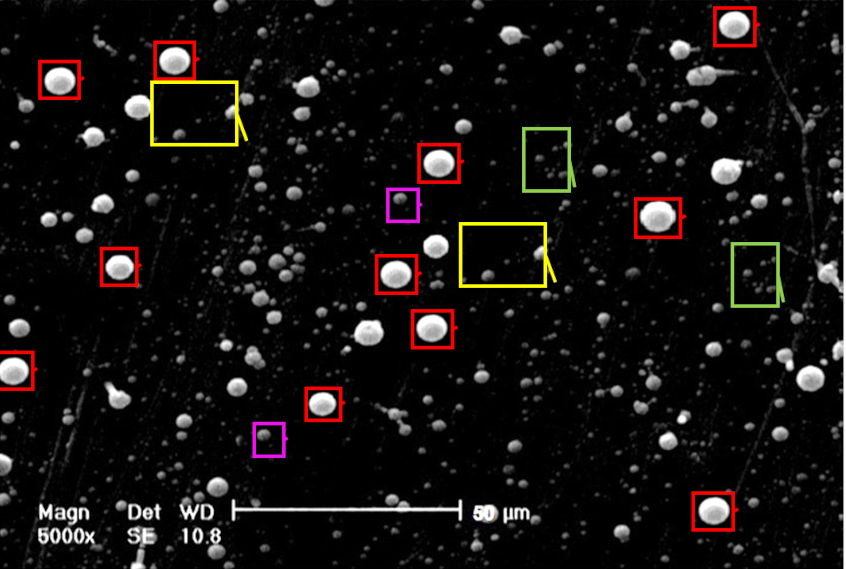
\includegraphics[width=0.8\textwidth]{img/pubpeer/pubpeer_dupes.PNG}
\end{figure}

\pagebreak
\begin{quote}
    \textit{Figure 6: Some of the images previously \href{https://pubpeer.com/publications/2E9CC5D00FDE41668A28B9622E64ED}{appeared elsewhere}. Identified by \href{https://imagetwin.ai}{Imagetwin.ai}.}
\end{quote}

\begin{figure}[h!tbp]
\centering
    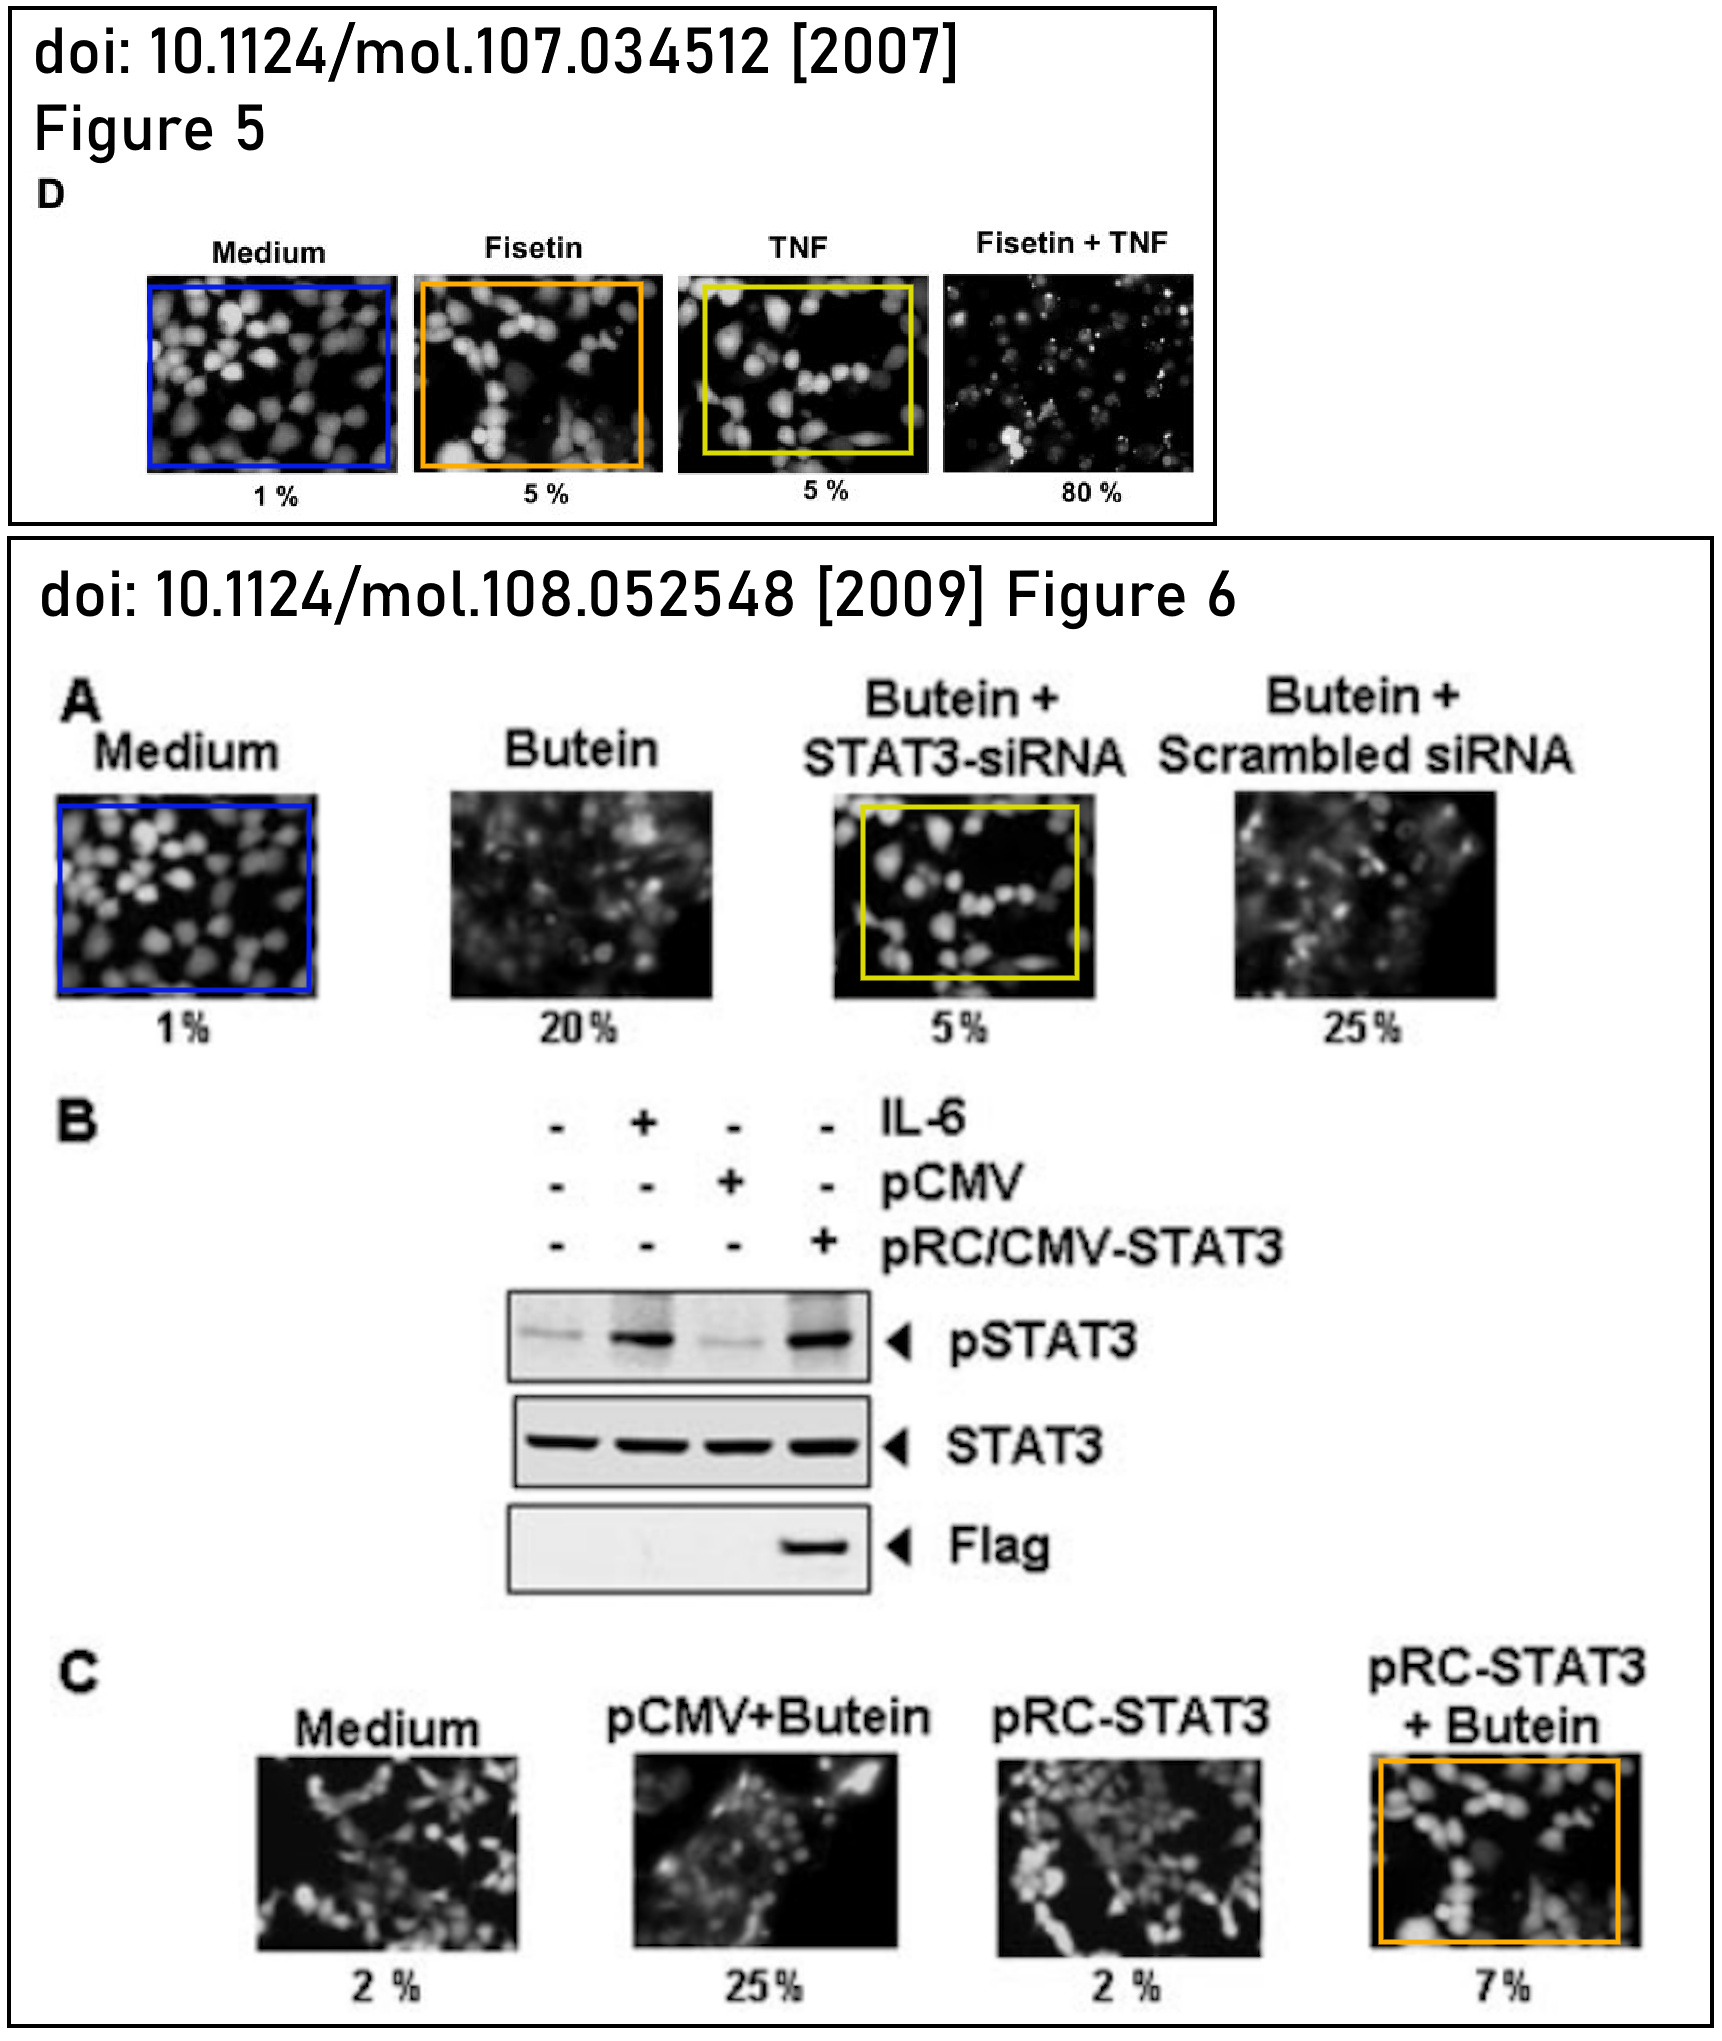
\includegraphics[width=0.5\textwidth]{img/pubpeer/image-1729709836291.png}
\end{figure}

\subsubsection*{Examples of unhelpful comments}

\begin{quote}
    \textit{The nanoparticles in Figure 8 look a bit wonky.}
\end{quote}

\begin{quote}
    \textit{Some of the lanes SDS-PAGE gel shown in Figure 4 look very similar to one another.}
\end{quote}

\subsection*{Do not speculate on researcher motivations}

Even when there is copious evidence that some fabrication, falsification or plagiarism occurred in a publication, it is not helpful to allege research misconduct. From the \href{https://pubpeer.com/static/faq#4}{PubPeer FAQ}:

\begin{quote}
    \textit{Allegations of misconduct are forbidden on PubPeer. They are anyway unnecessary. Your audience on the site is mostly composed of highly intelligent researchers and scientists. They are quite capable of drawing their own conclusions if the facts are clearly presented.}
\end{quote}

\begin{quote}
    \textit{You should also avoid personal comments about authors and speculation about researcher actions and motives. This is non-scientific, but also can pose legal problems.}
\end{quote}

Beyond this, it is often not possible to know exactly what took place in a publication's preparation and who was responsible for the improprieties observed in PubPeer comments.

\subsection*{Make specific, actionable requests from authors}

Authors are the best experts on their own publications and PubPeer has the option to provide author emails to loop them into a discussion. Questions about a publication can often be addressed directly by authors, so it is helpful to make clarifying requests where appropriate.

\begin{quote}
    \textit{Could the authors provide the original scanning electron microscope images shown in Figure 3?}
\end{quote}

\begin{quote}
    \textit{Could the authors provide the raw data for the EDX spectrum shown in Figure 4?}
\end{quote}

\begin{quote}
    \textit{Could the authors clarify how they estimated crystallite size?}
\end{quote}

\begin{quote}
    \textit{Could the authors clarify what ``enormous information'' means and why it was used instead of ``big data''?}
\end{quote}

\subsection*{Split multiple observations into multiple comments}

PubPeer comments can be referenced from other PubPeer comments on the same article by referring to the comment number preceded by ``\#''.

If you have many observations on different aspects of an article, consider splitting these observations into multiple comments so that other commenters can reference your specific observations one at a time.

\begin{figure}[h!tbp]
    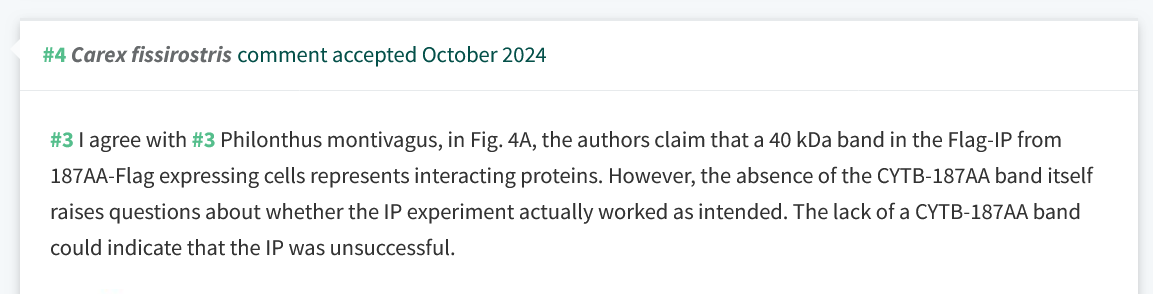
\includegraphics[width=\textwidth]{img/pubpeer/Screenshot 2024-10-23 at 16-36-04 PubPeer - A novel protein CYTB-187AA encoded by the mitochondrial gene.png}
    \caption*{This PubPeer comment refers back to a previous PubPeer comment using \#. The comment number for this comment can be found in the upper left corner of the comment box, to the left of the commenter's alias.}
\end{figure}
\end{document}
\documentclass[letterpaper, 12pt]{article}

\usepackage{geometry}
 \geometry{
 letterpaper,
 total={170mm,257mm},
 left=20mm,
 top=20mm,
 bottom=20mm
 }
\usepackage{graphicx} % Required for inserting images
\usepackage{authblk}
\usepackage{amssymb}
\usepackage{lipsum}
\usepackage{float}
\usepackage{times}
\usepackage{amsmath}
\usepackage[format=plain,
            labelfont={bf,it},
            textfont=it]{caption}
\captionsetup{justification=raggedright,singlelinecheck=false}
\usepackage{ragged2e}
\usepackage{longtable}
\usepackage{comment}
\usepackage{setspace}
\usepackage{fancyhdr}
\usepackage{titlesec}
\usepackage[hyperindex,breaklinks]{hyperref}
\hypersetup{
    colorlinks=true,
    linkcolor=blue,
    filecolor=magenta,      
    urlcolor=blue
    }
% \usepackage{background} % add COSIG logo to page
\usepackage[T1]{fontenc}
\usepackage{helvet}
\renewcommand{\familydefault}{\sfdefault}
\pagenumbering{gobble}
\usepackage[skip=10pt plus1pt, indent=40pt]{parskip}

\begin{comment}
\backgroundsetup{
   scale=1,
   angle=0,
   opacity=1,
   color=black,
   contents={\begin{tikzpicture}[remember picture, overlay]
      \node at ([xshift=3cm,yshift=1cm] current page.south west)
            {
\includegraphics[width = 5cm]{img/home/241017_final_logo_mockup.png}}; %<- change the name of image
     \end{tikzpicture}}
 }
\end{comment}

\titlespacing*{\section}
{0pt}{1.5ex plus 1ex minus .2ex}{1.3ex plus .2ex}

\renewcommand\Authfont{\fontsize{12}{14.4}\selectfont}
\renewcommand\Affilfont{\fontsize{9}{10.8}\itshape}
 
\begin{document}
\flushleft

\includegraphics[width=0.5\textwidth]{img/home/241017_final_logo_mockup.png}

\section*{Reporting publication integrity issues to publishers}
\addcontentsline{toc}{section}{Reporting publication integrity issues to publishers}
\textit{Last updated: 13 May 2025}

\subsection*{Integrity/ethics teams at publishers}

Most of the large scientific publishers have whole departments for publication ethics and publication integrity. These departments investigate incoming reports of possible errors and will advise editors and editors-in-chief on how to correct the scientific record. Usually these departments will follow the guidelines set by the \href{https://publicationethics.org/}{Committee on Publication Ethics (COPE)}, which generally consists of reviewing the evidence, contacting the journal and authors and coming to some sort of closure.

\subsection*{How to report issues to publishers}

The best way to reach these teams is by email. You can send this email both to the publisher's integrity team as well as to the journal's editors-in-chief. Some journals will have editorial board members that specifically handle ethics concerns or certain topics (e.g., disciplinary fields or specific methodologies).

Just as described in the guide for \href{https://osf.io/sghaq}{PubPeer commenting best practices}, you should be clear and neutral when describing potential publication integrity issues to these teams. Always include the \href{https://www.doi.org/}{DOI} (or other permanent identifier, such as PubMed ID) of the article(s) in question and report in a neutral way about the issue(s). Including a link to PubPeer where the issues are discussed in greater depth or an including an image to illustrate an issue may be useful.

Always be respectful when you contact publishers' integrity teams. Do not project frustrations or anger onto the members of these teams. Feel free to ask for a confirmation of receipt at the end of your email in order to make sure that the recipient has received all the relevant information.

\subsection*{Example of a helpful email to a publisher}

\begin{quote}
\textit{To whom it may concern,}\\
\indent\\
\textit{We have detected duplicated images in figures of articles published in [journal].}\\
\indent\\
\textit{We found an overlap between figure 1, panel A of Article 1 [DOI] and Figure 5, panel B of Article 2 [DOI]. We also found an overlap between Figure 3, panel C of Article 1 [DOI] and Figure 1, panel E of Article 3 [DOI].}\\
\indent\\
\textit{All of our findings have also been made publicly available on PubPeer:}\\
\indent\\
\textit{Article 1: [PubPeer link]\\
Article 2: [PubPeer link]\\
Article 3: [PubPeer link]\\}
\indent\\
\textit{Feel free to contact us with your questions. We’re happy to clarify any issues you might have. Could all of the recipients send us a confirmation of receipt of this email and let us know what the timeframe will be for assessing these issues?}\\
\indent
\textit{Best,}\\
\indent\\
\textit{[Name/pseudonym]}
\end{quote}

\subsection*{What happens next?}

You should be very patient after reporting an issue; investigations often take months if not years to resolve, even for blatant issues that seem to warrant immediate action. A publisher's integrity team may take one of several actions after being contacted regarding a publication integrity or ethics issue:

\begin{itemize}
    \setlength\itemsep{-0.5em}
    \item When an investigation finds that the conclusions of the research are not affected, the authors will be given the chance to clarify or correct their article post-publication. This will be often done in the form of a \textit{correction}, which should detail what the initial problem was and how the problem was resolved.
    \item When an investigation finds that conclusions of the research are affected or the work cannot be trusted, the article will usually be \textit{retracted}. A retraction note will be published, detailing why the problem was too substantial to correct.
    \item When it is unclear whether the conclusions are affected by the reported issue, an \textit{expression of concern} might be issued. This is a way for publishers to show that readers should exercise increased caution when interpreting the results of the published article.
    \item Nothing happens. Research integrity teams handle many cases and may drop a case with or without notifying the party that raised the issue.
\end{itemize}

When reporting an issue, you may ask to be notified when an investigation is resolved or an editorial notice is applied to an article. COPE \href{https://doi.org/10.24318/cope.2019.2.25}{recommends} that editors inform the person that originally raised concerns when the an outcome is reached, but many publishers fail to adhere to this guidance.

\pagebreak
\subsection*{Contact information for integrity/ethics teams at major publishers}

\begin{itemize}
    \setlength\itemsep{-0.5em}
    \item American Chemical Society (ACS): Each journal usually has contact information for a managing editor, usually at managing.editor@<journal-url>.org
    \item American Society for Microbiology: ethics.journals@asmusa.org
    \item British Medical Journal (BMJ): publication.ethics@bmj.com
    \item Elsevier (Elsevier, Cell Press): ethicsexpert@elsevier.com
    \item Frontiers: research.integrity@frontiersin.org
    \item IEEE: pub-ethics@ieee.org
    \item Karger: publication.ethics@karger.com
    \item MDPI: publication.ethics@mdpi.com
    \item Oxford University Press: journals.ethics@oup.com
    \item PLOS: pub-ethics@plos.org
    \item Rockefeller University Press (Journal of Cell Biology, Life Science Alliance): integrity@rupress.org
    \item Sage (Sage, Mary-Ann Liebert): publication\_ethics@sagepub.com
    \item Springer Nature (Springer, Nature, BMC): ethics.reporting@springernature.com
    \item Taylor \& Francis (Taylor \& Francis, Dove Medical Press, CRC Press, Routledge): ethics@tandf.co.uk
    \item Wiley (Wiley, Hindawi, FEBS Press): researchintegrity@wiley.com
\end{itemize}

\subsection*{Additional resources}

\begin{itemize}
    \setlength\itemsep{-0.5em}
    \item \href{https://doi.org/10.3145/epi.2023.ene.18}{``How do journals deal with problematic articles. Editorial response of journals to articles commented in PubPeer'' (2023)}
\end{itemize}

\end{document}
\documentclass[letterpaper, 12pt]{article}

\usepackage{geometry}
 \geometry{
 letterpaper,
 total={170mm,257mm},
 left=20mm,
 top=20mm,
 bottom=20mm
 }
\usepackage{graphicx} % Required for inserting images
\usepackage{authblk}
\usepackage{amssymb}
\usepackage{lipsum}
\usepackage{float}
\usepackage{times}
\usepackage{amsmath}
\usepackage[format=plain,
            labelfont={bf,it},
            textfont=it]{caption}
\captionsetup{justification=raggedright,singlelinecheck=false}
\usepackage{ragged2e}
\usepackage{longtable}
\usepackage{comment}
\usepackage{setspace}
\usepackage{fancyhdr}
\usepackage{titlesec}
\usepackage[hyperindex,breaklinks]{hyperref}
\hypersetup{
    colorlinks=true,
    linkcolor=blue,
    filecolor=magenta,      
    urlcolor=blue
    }
% \usepackage{background} % add COSIG logo to page
\usepackage[T1]{fontenc}
\usepackage{helvet}
\renewcommand{\familydefault}{\sfdefault}
\pagenumbering{gobble}
\usepackage[skip=10pt plus1pt, indent=40pt]{parskip}

\begin{comment}
\backgroundsetup{
   scale=1,
   angle=0,
   opacity=1,
   color=black,
   contents={\begin{tikzpicture}[remember picture, overlay]
      \node at ([xshift=3cm,yshift=1cm] current page.south west)
            {
\includegraphics[width = 5cm]{img/home/241017_final_logo_mockup.png}}; %<- change the name of image
     \end{tikzpicture}}
 }
\end{comment}

\titlespacing*{\section}
{0pt}{1.5ex plus 1ex minus .2ex}{1.3ex plus .2ex}

\renewcommand\Authfont{\fontsize{12}{14.4}\selectfont}
\renewcommand\Affilfont{\fontsize{9}{10.8}\itshape}
 
\begin{document}
\flushleft

\includegraphics[width=0.5\textwidth]{img/home/241017_final_logo_mockup.png}

\section*{Citations}
\addcontentsline{toc}{section}{Citations}
\textit{Last updated: 4 May 2025}

Science is built incrementally, one discovery at a time.
Scientific articles \emph{cite} other articles to make reference to previous work and claims.
\emph{Citations} are a core feature of all scientific papers.

Citations are typically short references in an article's text to entries in a ``References'' or ``Bibliography'' section,
which itself contains paper titles, author names, years, and so on.
Different journals and publishers adopt different \href{https://libguides.brown.edu/citations/styles}{styles of citations}, typically either numeric (e.g., ``[1]'', ``[42]'')
or author-year (e.g., ``[Smith 2024]'', ``[Garcia 1974b]''). Authors often cite multiple sources at once (e.g., ``Several studies have found that the $A$ is positively correlated with $B$ [Smith 2024, Rodriguez 2023, Wang 2022]'').

Counting the number of times an article has been cited is an imperfect measure of how influential an article might be since it usually indicates that others found at least some part of the paper useful or otherwise built upon the work described in the article.

Citation counting is also often used to measure the impact and influence of authors. For instance, authors are often judged by their \href{https://doi.org/10.1073%2Fpnas.0507655102}{$h$-index}.
Someone with an $h$-index of $N$ has published $N$ articles each cited at least $N$ times. Similarly, journals are often evaluated by how often the articles they publish are cited, such as through the \href{https://doi.org/10.1001%2Fjama.295.1.90}{journal impact factor (JIF)}. JIF roughly corresponds to the average number of citations each article receives within a certain time frame following publication. The only official source for JIF is \href{https://clarivate.com/academia-government/scientific-and-academic-research/research-funding-analytics/journal-citation-reports/}{Clarivate's Journal Citation Reports}, which uses the database \href{https://clarivate.com/academia-government/scientific-and-academic-research/research-discovery-and-referencing/web-of-science/}{Web of Science}.

Heuristics like $h$-index and JIF are \href{https://doi.org/10.1038/d41586-022-02984-2}{used frequently in academic hiring and promotion decisions} as proxies of researcher productivity and influence. As a result, it is generally desirable for academics to acquire a higher number of citations than their peers. Similarly, journal editors and publishers may seek to increase the number of citations to their journals' articles to augment their journals' reputations.

\subsection*{Expected citation behavior}

Any claim that is not ``common sense'' or ``common knowledge'' generally requires a citation, although this is context-dependent.
Citations can reference a specific claim from a source (e.g., ``Less than 40\% of frobnicators are red [Zhang 2003]''). 
Citations can also point to a previous work as an example (e.g. ``We measure frobnication using the standard XYZ technique [24]'').
For basic claims that would be common knowledge among an article's likely readers (e.g., ``DNA is double-stranded'' or ``computers use binary digits'')
no citation is necessary.

\subsection*{Problematic citation behavior}

Citations can be problematic for a number of reasons. Some problematic citations behaviors are quite common and may not represent intentional distortions. For instance, authors may claim something about a cited article that is untrue or is unsupported by the cited article's text. On the other hand, other problematic citation behaviors are the direct result of \href{https://doi.org/10.24318/cope.2019.3.1}{citation manipulation} intended to inflate the previously-described citation metrics.

\subsection*{Archetypes of common problematic citation behaviors}

This section describes common issues that can be found among an article's citations, as well as possible motivations and explanations for these issues. Relevant examples are provided for each. Note that these behaviors are not mutually exclusive.

\subsubsection*{Missing citations}

When making claims or showing data that was not the result of the authors' original research work, authors should cite their sources. Often, this does not actually occur.

(\href{https://pubpeer.com/publications/8A2CF2E1EBFD3ADCD835ADB91DDFE8}{example})

\subsubsection*{Citations that do not accurately reflect the content of the cited article}

Statements containing citations often do not accurately reflect what is actually contained in the cited article. It is commonplace (but nonetheless problematic) for authors to \href{https://ori.hhs.gov/citing-sources-were-not-read-or-thoroughly-understood}{cite articles that they haven't actually thoroughly read}.

(\href{https://pubpeer.com/publications/6E8756FAB18C392065D8313D271090}{example 1}, \href{https://pubpeer.com/publications/D3E493ADF94B3031D24C280F54F37E}{example 2})

\subsubsection*{Many citations at once}

More than a handful of citations to back up a single statement can be excessive. This practice can be especially problematic if these blocks of citations contain many citations to the same author or are mostly irrelevant to the statement being made.

(\href{https://pubpeer.com/publications/D6A50C6DD455715DE626C1CC56B8EB}{example 1}, \href{https://pubpeer.com/publications/11C10949E0FF4EA3C31B6A45F4E22C}{example 2})

\subsubsection*{Many citations to the same author}

More than a handful of citations to the same author in a paper is unusual. This can occur naturally if most of the previous scholarship on a topic is by the same author. However, this can also be an indication of a deliberate effort to inflate particular authors' citation metrics. 

(\href{https://pubpeer.com/publications/0C7C1F371CB05161EEACC303692521}{example})

\subsubsection*{Many self-citations}

Consistently citing the authors' own papers is problematic. Most citation metrics explicitly exclude self-citations.

(\href{https://pubpeer.com/publications/3EAC0C5735F8D48FF1D4B06C6BFC30}{example})

\subsubsection*{Unused citations}

Citations are typically expected to be used in the paper's main text, so references that only appear in an article's bibliography can be suspicious.

(\href{https://pubpeer.com/publications/0C7E7F2703724338046FF2A0AA8392}{example})

\subsubsection*{Overly specific citations}

Citing very specific applications of a concept instead of a definition or review of the concept is strange, especially for fundamental concepts.

(\href{https://pubpeer.com/publications/5A064B2F4AE7F13D6E1F559F84492F}{example})

\subsubsection*{Unrelated/irrelevant citations}

Citing articles that have nothing to do with the statement for which they are cited (\emph{citation context}) is inherently problematic.

(\href{https://pubpeer.com/publications/B9CE2B145B02E439BA9C5B2C2D5F12}{example 1}, \href{https://pubpeer.com/publications/C21D670DD4C94B02C78809A55ED385}{example 2})

\subsubsection*{``Suggested'' citation batches}

Reviewers who consistently ask authors to cite many of the reviewer's papers are, at best, in an ethical gray area. Authors will often include reviewers' and editors' suggested citations in the hopes of passing through peer review.

(\href{https://pubpeer.com/publications/90719DBC6E5FF2AC32FDE74F1A6A7F}{example 1}, \href{https://pubpeer.com/publications/1924F147DE045B97261004EB2387AE}{example 2})

\subsubsection*{Citation magnets}

The same paper cited in irrelevant or barely relevant contexts across many papers,
especially within the same venue, is an indication something is deeply wrong.  Such ``citation magnets'' are often cited alongside other citation magnets. Their presence among a paper's references can be indicative of paper milling and authorship-for-sale.

(\href{https://pubpeer.com/search?q=%22A+novel+Aluminum%E2%80%93graphite+dual-Ion+battery%22}{example 1}, cited 1,638 times, for which some of the citing articles were also implicated in \href{https://pubpeer.com/publications/DF9A5CE25CF36DDAFF4B6695B91EA7}{authorship-for-sale}; \href{https://pubpeer.com/publications/B71DD139D3549DCCA37DCEC8AF59D5}{example 2}, cited 49 times;  \href{https://docs.google.com/spreadsheets/d/1o-9OIyzZ9mMqA7bprcbI5nemtYBfxiXH1ndI3y5A43E/edit?usp=sharing}{a spreadsheet of likely citation magnets})

\subsubsection*{Citations that were not intended by the authors}

Authors often deny having inserted certain citations in their article.

(\href{https://pubpeer.com/publications/8DC24BCCDA68EC1954E1FCA74FDB8E\#2}{example})

\subsubsection*{Tortured titles}

Some ``plagiarism avoidance'' software will paraphrase text in a way that results in \href{https://arxiv.org/abs/2107.06751}{tortured phrases} (for more information, see the \href{https://osf.io/ntcb4}{COSIG plagiarism guide}). Sometimes, citation titles are also paraphrased, resulting in the title of an article, as it appears in the bibliography section, not matching the actual published title of an article.

(\href{https://pubpeer.com/publications/CF328DB7A6131B99F9805B49643D81\#2}{example})

\subsubsection*{Large-language model (LLM) ``hallucinations'' and fabrications}

LLM tools like ChatGPT often cite non-existent articles.

(\href{https://pubpeer.com/publications/8D6BF963665181144EC553BE2FDA92\#2}{example 1},
\href{https://web.archive.org/web/20230623093222/https://www.theguardian.com/technology/2023/jun/23/two-us-lawyers-fined-submitting-fake-court-citations-chatgpt}{example 2}, from outside of academic publishing)

\subsubsection*{Outdated citations}

An article may not cite the most up-to-date literature on a topic. Newer literature may have since expanded upon or directly refuted the claims made in older literature. Citing older articles is not necessarily an issue unless there is evidence that newer work has made the older work obsolete.

(\href{https://doi.org/10.1177/00315125241311636}{this retraction notice} lists one reason for the retractions as ``[antiquated] reference lists: Cited literature within these articles cited was, on average, 10–20 years prior to the authors’ publications''.)

\subsubsection*{Citations to retracted articles}

A cited article can be a problematic or unreliable source of information for a variety of reasons. An article being retracted is a reflection of this. As a result, it is often problematic for an article to rely on conclusions from retracted research (as indicated through their citations). See the \href{https://osf.io/9q3as}{COSIG entry dedicated to citations to retracted articles}.

\subsubsection*{Citations to hijacked journals}

Citations to articles published in hijacked journals are problematic. Hijacked journals often publish low-quality, non–peer-reviewed articles and are frequently associated with  misconduct (see the section on hijacked journals in COSIG's guide on \href{https://osf.io/vrk7e}{suspicious publication venues}). Hijacked journals will often publish content that is wildly outside of the journal's stated scope since they tend to publish anything in exchange for a fee.

The \href{https://dbrech.irit.fr/pls/apex/f?p=9999:27::::::}{Problematic Paper Screener's Citejacked detector} tracks articles that make citations to a selection of journals that have been hijacked.

\subsection*{Common false alarms}

\subsubsection*{Many relevant citations}

Some authors go a bit overboard with
relevant citations out of enthusiasm. If no other red flag applies,
this is probably not problematic.

\subsubsection*{Relevant, but occasional, suggested citations}

Reviewers are typically experts in their subfield. It is innocuous for reviewers to occasionally suggest citations to their own works, especially when such works are the definitive sources for a claim.

\subsubsection*{Occasional unused citations}

Various software glitches can result in a bibliography not being updated along with the paper text.
If one or two references appear only in the bibliography, but no other red flag applies, there is usually no cause for concern, although it may merit a correction.

\subsubsection*{Mistaken author names}

Some styles of last name are often abbreviated incorrectly in bibliography sections.
For instance, someone unfamiliar with French names might cite the former defense minister of France as ``Drian, Jean-Yves L.''
when in fact ``Le Drian'' is a single family name. Reference managers might also treat the names of consortia as single authors (e.g., ``Open Science Collaboration'' being abbreviated as ``Collaboration, OS''.)

\subsection*{Advanced cases}

\subsubsection*{Sneaked references}

What appears as a citation to human readers and what citation-counting software considers a citation may not match.
Literature aggregation databases have been cheated in the past to increase citation counts in a way that is not detectable from just paper texts alone, in a practice known as \href{https://doi.org/10.1002/asi.24896}{``sneaking references''}.

\subsubsection*{Hidden authors}

To save space, some venues require papers with more than a few authors to be abbreviated using ``et al.'',
such as ``Diallo, A., Nikolov, B., et al.''.
This can be used to conceal the fact that many cited papers have authors in common.

(\href{https://pubpeer.com/publications/00DCF18F504B8C420F12A70B5FB30C}{example})

\subsubsection*{Vicker's curse}

One notorious citation magnet \href{https://forbetterscience.com/2022/10/31/when-im-citing-you-will-you-answer-too/}{described first in 2022} is the 2017 editorial \href{https://doi.org/10.1016/j.cub.2017.05.064}{``Animal Communication: When I’m Calling You, Will You Answer Too?''} by Neil J. Vickers, which has been cited as many as 2000 times in contexts completely irrelevant to its subject matter (moth pheromones). Articles featuring this irrelevant citation were said to be afflicted by ``Vicker's curse''. In 2023, \href{https://forbetterscience.com/2023/07/31/the-vickers-curse-secret-revealed/}{it was discovered} that this article was often the first to appear when an incomplete digital object identifiers (DOIs) was entered into the searchbar on Google Scholar (specifically, the string ``10.1016/j.'' the prefix for many article DOIs used by Elsevier). There are \href{https://pubpeer.com/publications/4BB5BE5F56EFEBC3A67D89D1EB5501}{other probable examples} of citation magnets that result from searching incomplete DOIs. 

\subsection*{Additional resources}

\begin{itemize}
    \setlength\itemsep{-0.5em}
    \item \href{https://doi.org/10.24318/cope.2019.3.1}{COPE discussion document on citation manipulation}
    \item \href{https://osf.io/9q3as}{COSIG: Citations to retracted publications}
\end{itemize}

\end{document}
\documentclass[letterpaper, 12pt]{article}

\usepackage{geometry}
 \geometry{
 letterpaper,
 total={170mm,257mm},
 left=20mm,
 top=20mm,
 bottom=20mm
 }
\usepackage{graphicx} % Required for inserting images
\usepackage{authblk}
\usepackage{amssymb}
\usepackage{lipsum}
\usepackage{float}
\usepackage{times}
\usepackage{amsmath}
\usepackage[format=plain,
            labelfont={bf,it},
            textfont=it]{caption}
\captionsetup{justification=raggedright,singlelinecheck=false}
\usepackage{ragged2e}
\usepackage{longtable}
\usepackage{comment}
\usepackage{setspace}
\usepackage{fancyhdr}
\usepackage{titlesec}
\usepackage[hyperindex,breaklinks]{hyperref}
\hypersetup{
    colorlinks=true,
    linkcolor=blue,
    filecolor=magenta,      
    urlcolor=blue,
    pdftitle={Overleaf Example},
    pdfpagemode=FullScreen,
    }
% \usepackage{background} % add COSIG logo to page
\usepackage[T1]{fontenc}
\usepackage{helvet}
\renewcommand{\familydefault}{\sfdefault}
\pagenumbering{gobble}
\usepackage[skip=10pt plus1pt, indent=40pt]{parskip}

\begin{comment}
\backgroundsetup{
   scale=1,
   angle=0,
   opacity=1,
   color=black,
   contents={\begin{tikzpicture}[remember picture, overlay]
      \node at ([xshift=3cm,yshift=1cm] current page.south west)
            {
\includegraphics[width = 5cm]{img/home/241017_final_logo_mockup.png}}; %<- change the name of image
     \end{tikzpicture}}
 }
\end{comment}

\titlespacing*{\section}
{0pt}{1.5ex plus 1ex minus .2ex}{1.3ex plus .2ex}

\renewcommand\Authfont{\fontsize{12}{14.4}\selectfont}
\renewcommand\Affilfont{\fontsize{9}{10.8}\itshape}
 
\begin{document}
\flushleft

\includegraphics[width=0.5\textwidth]{img/home/241017_final_logo_mockup.png}

\section*{Citations to retracted publications}
\addcontentsline{toc}{section}{Citations to retracted publications}
\textit{Last updated: 16 April 2025}

References to retracted publications can pose a reliability issue in scientific literature since retractions indicate that a publication has been found unreliable. Citations/references to such articles can disseminate unreliable information in the scientific literature. It is stated in \href{https://www.icmje.org/icmje-recommendations.pdf}{Recommendations for the Conduct, Reporting, Editing, and Publication of Scholarly Work in Medical Journals} that authors are responsible for checking that none of the references cite retracted articles except in the context of referring to the retraction. 
However, not all retracted articles are cited after their retraction (post-retraction citations), and not all citations serve the same purpose. It is important to consider the context in which a retracted paper is cited. A retraction in the references does not automatically make all citing papers unreliable, but citations to retracted publications can serve as a fingerprint for identifying potential issues in the literature. This guide provides information about how to identify such citations and what nuances should be considered in the analysis and reporting of these cases. 

\subsection*{Identifying citations to retracted publications}
The \href{https://dbrech.irit.fr/pls/apex/f?p=9999:31}{Problematic Paper Screener’s Feet of Clay Detector} is a dynamic tool that identifies and maintains an updated record of publications that may be unreliable as they cite one or more  retracted/removed/withdrawn references spotted by the \href{https://www.irit.fr/~Guillaume.Cabanac/problematic-paper-screener/annulled}{Annulled Detector}. However, one limitation of this detector is that it does not provide further assessment regarding the extent to which the credibility of a citing work is affected by the fact that it cites retracted articles. Because of this, the tool has a feedback feature to identify false positive cases (e.g., a retracted work was cited and criticized, or the retraction is acknowledged). For true positives (e.g., a retracted work’s data was used by or central to the citing work), PubPeer comments are encouraged. 

\subsection*{Why was the cited publication retracted?} 

Retractions can happen for non-scientific content related reasons. This can potentially reduce the idea of ‘propagation of unreliable science’. The \href{https://retractionwatch.com/retraction-watch-database-user-guide/retraction-watch-database-user-guide-appendix-b-reasons/}{Retraction Watch Database User Guide Appendix B: Reasons} describes various common reasons why retractions occur. For example, if an article was retracted based on the content of the publication (e.g., retraction reasons ``error in data/analyses'', ``error in cell lines'') can imply a potential reliability issue for the citing work if the data and analyses of this publication were a central part of the citing work. This information is particularly helpful when analyzing large amounts of citations since it can be obtained from the joint database of \href{https://gitlab.com/crossref/retraction-watch-data}{Retraction Watch and Crossref}. For case-by-case analyses, retraction notices can provide more detailed and accurate information about reasoning. 

\subsection*{Post- and pre-retraction citations}

Publications may be cited after they are retracted (post-retraction citation), or they might have been cited before they were retracted (pre-retraction citation). 
It is feasible to allow one year gap after retraction before considering a citation to be post-retraction (retraction notices take time to appear on journal sites and bibliometric databases and are often \href{https://retractionwatch.com/2024/07/05/how-you-can-help-improve-the-visibility-of-retractions-introducing-nisos-recommended-practice-for-communication-of-retractions-removals-and-expressions-of-concern-crec/}{not prominent at all}). \href{ https://doi.org/10.1162/qss_a_00155}{Hsiao and Schneider, 2022} discuss different parameters used in the systematic analyses of citations to retracted publications. We refer to this paper to add further specific examples.  

Post-retraction citations are likely not problematic for the citing work if the retraction is acknowledged by the authors, if the work is used to be criticized or questioned or is shown as an example of `bad science'. It is also important to be aware of whether or not the post-retraction citation is a self-citation (i.e., by the same authors or same research group) since this can be particularly problematic; in these cases, the odds are higher that retraction of the cited work was outright ignored. For pre-retraction citations, which are much more common in the literature, it is important that the authors are aware of the status of their references to reflect back on the use of these works. 

\subsection*{How is the retracted work cited?}

When reporting these cases on PubPeer or providing feedback on the Feet of Clay Detector, it is important to dig a bit deeper in the citing works to understand the purpose the citation in the citing work. It is important to consider the full-text to retrieve the citation context (the sentence/section in which the citation occurs). Only by access to this context can one identify if the cited retracted work is used in the methodology/approach of the citing work, which could be especially problematic. On the other hand, a retracted work could be cited as part of a passing mention of related works or as basic background information. This usually does not imply an unreliability issue for the citing work. 

\subsection*{Quantity of citations to retracted works}

It is common to see PubPeer comments focused on the quantity or frequency of citations to retracted or otherwise questionable publications within a citing work, rather than looking at the specific contexts (which often require significant domain expertise and time). These comments can be strengthened with more evidence from the citing paper. 

\subsection*{Example 1: Dozens of citations to retracted articles}
\href{https://doi.org/10.1007/s12094-019-02104-z}{Viera et al. (2019)} performed a review of the literature on microRNA signatures in childhood sarcomas. Of 637 references in the work, more than 60 are to retracted publications, at least two of which were retracted at the time of publication. An \href{https://doi.org/10.1007/s12094-024-03518-0}{expression of concern} was published for the article in 2024, highlighting an over-reliance on retracted works.
%(Yagmur: I can later on update this part with my PMC sentence extraction and discourse analysis pipeline once it’s on github/after I receive reviews)
\subsection*{Example 2: Retraction due to citing retracted work}
\href{http://dx.doi.org/10.2174/157488606775252629}{Iwamoto et al. (2006)} reviewed the literature on the use of vitamin K2 in the treatment of postmenopausal osteoporosis. This review was subsequently retracted (at a date not included in the retraction notice) for references to thee retracted works (out of 45 references), two of which were also authored by the authors of the review. These articles were retracted years after the publication of the review. The retraction notice states that ``[the] citation of these papers in this article seriously undermines the authenticity and integrity of the content presented''.

\subsection*{Example 3: Citing work is about the retraction of the cited work}
\href{https://doi.org/10.4155/cli.14.116}{George and Buyse (2015)} review several prominent cases of fraud in clinical trials. In this context, they cite a retracted article by \href{https://doi.org/10.1016/S0140-6736(05)67488-0}{Sudb\o{} et al. (2005)}.

\subsection*{Example 4: Citing work acknowledges the retraction of the cited work}
\href{https://pmc.ncbi.nlm.nih.gov/articles/PMC3320713/}{Varadhan et al. (2012)} perform a meta-analysis on the safety and efficacy of antibiotics for acute appendicitis. They explain ``[the] meta-analysis presented here provides a valid and up to date summary of the relevant literature [...] It excludes the study that has been retracted subsequent to publication [REF]'', citing a retracted study by \href{https://doi.org/10.1007/s11605-009-0835-5}{Malik and Bari (2009)}. 

\subsection*{Example 5: Citing work is not impacted by the cited retracted work}

Not all cited retracted works will have an impact on the citing work. For example, one retracted work is cited only once in the introduction section of \href{https://doi.org/10.7150/thno.51231}{Ye et al. (2020)} as ``Previous studies demonstrated that the m\textsuperscript{6}A modification was correlated with carcinogenesis, tumor proliferation and chemoresistance of cancer cells [REFs]''. Multiple references are used (that are not retracted) to support this statement. This citation does not significantly impact the citing work or influence the content of the article itself.

\begin{comment}
\subsection*{Example 5: Citing work is not "scientifically" impacted by the cited retracted work}

There are no strict criteria for how a citation ``impacts'' the citing work; this must be evaluated on a case-by-case basis. of how can we identify the "impact" but the questions we have mentioned above can help in this decision. This \href{https://pubpeer.com/publications/9F571982CF73571F41D7E533AF4A38}{example} is about a monograph that heavily cites retracted publications. However, upon further inspection, the monograph's content is not original research but more of an extensive review. Some of the retracted resources are cited in tables to compare results among different works, or when it is found in the body text, it is only to show background work. Readers should be aware that references are unreliable, but it is questionable whether or not these references make the work itself scientifically unreliable, especially when we consider the retraction reasons. Such cases are usually observed in review articles is put into question in this \href{https://pubpeer.com/publications/8033BE0DEBC4DDCEF56B140A91F426}{example}.  
\end{comment}

\begin{comment}
\subsection{Commenting on PubPeer about Citations to Retracted Publications}
%Yagmur: input from Guillaume here?
\end{comment}

\subsection*{Additional resources}

\begin{itemize}
    \setlength\itemsep{-0.5em}
    \item \href{https://dbrech.irit.fr/pls/apex/f?p=9999:31::::::}{The Problematic Paper Screener: Feet of Clay Detector}
    \item \href{https://direct.mit.edu/qss/article/2/4/1144/107356/Continued-use-of-retracted-papers-Temporal-trends}{``Continued use of retracted papers: Temporal trends in citations and (lack of) awareness of retractions shown in citation contexts in biomedicine'' (2022)}
    \item \href{https://doi.org/10.1378/chest.11-0523}{``Exclusive: the papers that most heavily cite retracted studies'' (2024)}
    \item \href{https://jamanetwork.com/journals/jamainternalmedicine/article-abstract/2831911}{``Inclusion of Retracted Studies in Systematic Reviews and Meta-Analyses of Interventions: A Systematic Review and Meta-Analysis'' (2025)}
\end{itemize}

\end{document}
\documentclass[letterpaper, 12pt]{article}

\usepackage{geometry}
 \geometry{
 letterpaper,
 total={170mm,257mm},
 left=20mm,
 top=20mm,
 bottom=20mm
 }
\usepackage{graphicx} % Required for inserting images
\usepackage{authblk}
\usepackage{amssymb}
\usepackage{lipsum}
\usepackage{float}
\usepackage{times}
\usepackage{amsmath}
\usepackage[format=plain,
            labelfont={bf,it},
            textfont=it]{caption}
\captionsetup{justification=raggedright,singlelinecheck=false}
\usepackage{ragged2e}
\usepackage{longtable}
\usepackage{comment}
\usepackage{setspace}
\usepackage{fancyhdr}
\usepackage{titlesec}
\usepackage[hyperindex,breaklinks]{hyperref}
\hypersetup{
    colorlinks=true,
    linkcolor=blue,
    filecolor=magenta,      
    urlcolor=blue
    }
% \usepackage{background} % add COSIG logo to page
\usepackage[T1]{fontenc}
\usepackage{helvet}
\renewcommand{\familydefault}{\sfdefault}
\pagenumbering{gobble}
\usepackage[skip=10pt plus1pt, indent=40pt]{parskip}

\titlespacing*{\section}
{0pt}{1.5ex plus 1ex minus .2ex}{1.3ex plus .2ex}

\renewcommand\Authfont{\fontsize{12}{14.4}\selectfont}
\renewcommand\Affilfont{\fontsize{9}{10.8}\itshape}
 
\begin{document}
\flushleft

\includegraphics[width=0.5\textwidth]{img/home/241017_final_logo_mockup.png}

\section*{Formulaic research}
\addcontentsline{toc}{section}{Formulaic research}
\textit{Last updated: 31 May 2025}

Many research fields have seen recent explosions in the number of articles performing what could be described as ``formulaic'' research. Such articles often follow a similar template and similar methods and are only differentiated by the exact variable, outcome, disease, subject, etc. that has been swapped in. This strain of research has been described as ``cut-and-paste research'' and \href{https://doi.org/10.1126/science.zgawnij}{``research Mad Libs\textregistered''}. 

This guide describes several fields that have recently seen a large number of formulaic research articles published. Many are suspected to result from the activity of research paper mills, organizations that are known to sell authorship on mass-produced manuscripts.

When evaluating any manuscript, some helpful questions to ask include:

\begin{itemize}
    \setlength\itemsep{-0.5em}
    \item Is the hypothesis well-justified?
    \item Are the methodological specifics (e.g., inclusion/exclusion criteria) well-justified?
    \item Does this work seem to resemble a previous work with only minor variations?
    \item Does this work control for possible false discoveries (see COSIG's \href{https://osf.io/csxd5}{entry on multiple hypothesis correction})?
\end{itemize}

\subsection*{Example 1: Mendelian randomization studies}

\href{https://doi.org/10.1038/s43586-021-00092-5}{Mendelian randomization (MR)} is an epidemiological method that leverages genotype information in large-scale cohorts (e.g., the \href{https://www.ukbiobank.ac.uk/}{UK Biobank}) to study the causal relationship between an exposure (e.g., physical activity, drinking coffee, etc.) and an outcome (e.g., Alzheimer's disease, type II diabetes, etc.). \href{https://doi.org/10.1093/ije/dyx028}{Two-sample MR (2SMR)} is a variant of MR that relies solely on summary statistics, typically from \href{https://doi.org/10.1038/s43586-021-00056-9}{genome-wide associations studies (GWAS)}. Recently, thousands of poor-quality \href{https://doi.org/10.1093/ije/dyx028}{two-sample MR (2SMR)} studies have been published, likely aided by the accessibility of large genetic databases and the availability of user-friendly interfaces for interacting with this data (e.g., the R packages \href{https://doi.org/10.7554/eLife.34408}{TwoSampleMR} and \href{https://doi.org/10.12688/wellcomeopenres.19995.2}{MendelianRandomization}). These studies often only report a 2SMR study with no additional supporting evidence for an association and feature weakly-motivated hypothetical associations (such as an association between \href{http://dx.doi.org/10.3389/fendo.2024.1396032}{air pollution and non-alcoholic fatty liver disease} or \href{http://dx.doi.org/10.3390/nu15092091}{noodle consumption and metabolic syndrome}).

\subsubsection*{Additional resources}

\begin{itemize}
    \setlength\itemsep{-0.5em}
    \item \href{https://doi.org/10.1186/s12944-024-02284-w}{``Reclaiming mendelian randomization from the deluge of papers and misleading findings'' (2024)}
    \item \href{https://doi.org/10.1136/egastro-2025-100187}{``Attention to the misuse of Mendelian randomisation in medical research'' (2025)}
    \item \href{https://doi.org/10.1016/S2213-8587(23)00348-0}{``Mendelian randomisation at 20 years: how can it avoid hubris, while achieving more?'' (2024)}
\end{itemize}

\subsection*{Example 2: Associative research using National Health and Nutrition Examination Survey (NHANES) data}

The \href{https://www.cdc.gov/nchs/nhanes/index.html}{National Health and Nutrition Examination Survey (NHANES)} is a survey of thousands of United States adults and children conducted annually by the Centers for Disease Control and Prevention (CDC), who have made the data freely available since 1999. The data includes surveys, health exams and laboratory tests. Thousands of studies have been published analyzing NHANES data. However, recent years have seen a proliferation of studies performing formulaic single-factor analysis using NHANES data, often on unjustifiably small slices of the surveyed population and only over a limited number of years. For instance, \href{https://doi.org/10.3389/fendo.2023.1245199}{Nie et al. (2023)} analyze a hypothetical association between systematic immune-inflammation index and diabetes but only over the four years 2017 to 2020 while suitable data was available for the 21 years between 1999 and 2020.

Many of these studies report on specious hypotheses with little statistical support. These studies also recycle a small number of statistical methods, especially logistical regression, use of cubic splines, or further subdividing populations into quartiles, in order to cross statistical thresholds. For instance, \href{https://doi.org/10.1186/s12888-023-04935-1}{Zhang et al. (2023)} report on an association between higher serum albumin concentration and depressive symptoms with an odds ratio of 0.98 (95\% confidence interval 0.95-0.99) and a p-value of 0.037.

\subsubsection*{Additional resources}

\begin{itemize}
    \setlength\itemsep{-0.5em}
    \item \href{https://doi.org/10.1371/journal.pbio.3003152}{``Explosion of formulaic research articles, including inappropriate study designs and false discoveries, based on the NHANES US national health database'' (2025)}
\end{itemize}

\subsection*{Example 3: Bibliometric analyses}

\href{https://en.wikipedia.org/wiki/Bibliometrics}{Bibliometrics/scientometrics} is the quantitative study of indicators of knowledge transfer and development. One such indicator of knowledge transfer is citations between scientific articles. The number of citations an article has received is often used as a heuristic of that article's importance or quality and is a common analytical variable in bibliometric analyses. While high-quality \href{https://en.wikipedia.org/wiki/Metascience}{metascientific} research routinely uses such heuristics, the accessibility of bibliometric data through services like \href{https://scopus.com}{Scopus} and \href{/https://webofscience.com/}{Web of Science} makes it an easy target for low-quality, formulaic research articles. 

For instance, thousands of articles have been published where the authors report on characteristics of the N highest-cited article in a particular field (e.g., \href{https://doi.org/10.1097/coa.0000000000000021}{``A Bibliometric Analysis of the 100 Most Cited Articles in Cornea'', 2023}, \href{https://doi.org/10.3389/fphar.2022.963032}{``A bibliometric analysis of the 100 most-cited articles on curcumin'', 2022}). Such articles often report summary statistics of these top-cited articles (such as describing the distribution of countries of origin), but more often than not without comparison to a control group or to all other articles in the field, giving these quantitative analyses little analytical value.

Formulaic metascience articles can also report on author characteristics in any selected field of the scientific literature. For instance, \href{https://doi.org/10.7759/cureus.47208}{Djahanshahi et al. (2023)} report on gender trends among first authors in the scientific literature on \href{https://en.wikipedia.org/wiki/Wolff%E2%80%93Parkinson%E2%80%93White\_syndrome}{Wolff–Parkinson–White syndrome}, a rare heart disease for which fewer than 200 articles have been written. The authors' reasoning for selecting such a narrow field for analysis is unclear.

\subsubsection*{Additional resources}

\begin{itemize}
    \setlength\itemsep{-0.5em}
    \item \href{https://reeserichardson.blog/2024/12/30/recent-encounters-with-atom-thin-salami-slicing/}{``Recent encounters with atom-thin salami slicing: Case \#2: Same paper mill, same procedure, different subject, different authors'' (2024)}
\end{itemize}

\subsection*{Example 4: Querying a large language model}

Since the public release of \href{https://en.wikipedia.org/wiki/ChatGPT}{ChatGPT} in 2022, thousands of \href{https://scholar.google.com/scholar?start=10&q="conversation+with+chatgpt"+OR+"interview+with+chatgpt"&hl=en}{``conversations'' and ``interviews'' with ChatGPT} have been published in peer-reviewed and non-peer-reviewed outlets. These commentary pieces can be written with little effort on practically any scientific topic. Many are severely limited in scope, typically only sharing a single chain of queries and outputs on a single topic, and do little to interrogate the veracity of the large language model's responses to the user's queries. Moreover, because the companies that develop these models publicly release new versions and quietly make updates between official versions, these conversations are typically not reproducible and any insights gained from them quickly obsolesce.

\subsection*{Example 5: Non-coding RNAs}

Many suspected paper mill products, especially those in the field of \href{https://en.wikipedia.org/wiki/Non-coding_RNA}{non-coding RNAs} and disease, resemble variations on a theme. Plausible-sounding papers can be generated by combining just about any non-coding gene with any human disease and any molecular pathway. This pattern can even be observed in article titles alone, as noted for a collection of papers dubbed the \href{https://scienceintegritydigest.com/2020/02/21/the-tadpole-paper-mill/}{``Tadpole paper mill''}.

\begin{table}[h!tbp]
\scriptsize
\centering
\begin{tabular}{ccccccc}
  \textbf{\begin{tabular}[c]{@{}c@{}}Insert the name\\of a molecule\end{tabular}} &
  \textbf{\begin{tabular}[c]{@{}c@{}}Pick a verb\\(present tense,\\third person\\singular form)\end{tabular}} &
  \textbf{\begin{tabular}[c]{@{}c@{}}Choose\\one or two\\cellular\\processes\end{tabular}} &
  \textbf{\begin{tabular}[c]{@{}c@{}}Pick a\\cancer or\\cell type\end{tabular}} &
  \textbf{\begin{tabular}[c]{@{}c@{}}Pick your\\connector\\word\end{tabular}} &
  \textbf{\begin{tabular}[c]{@{}c@{}}Choose a verb\\(present\\particle form)\end{tabular}} &
  \textbf{\begin{tabular}[c]{@{}c@{}}Insert name\\of miRNA\\or pathway\end{tabular}} \\ \\ \hline
  \multicolumn{1}{|c|}{\begin{tabular}[c]{@{}c@{}}<protein name>\\<drug name>\\<RNA name>\end{tabular}} &
  \multicolumn{1}{c|}{\begin{tabular}[c]{@{}c@{}}alleviates\\attenuates\\exerts\\governs\\inhibits\\prevents\\promotes\\protects\\relieves\\remits\\retards\\suppresses\end{tabular}} &
  \multicolumn{1}{c|}{\begin{tabular}[c]{@{}c@{}}apoptosis\\autophagy\\inflammation\\invasion\\migration\\proliferation\\ viability\end{tabular}} &
  \multicolumn{1}{c|}{\begin{tabular}[c]{@{}c@{}}lung cancer\\medulloblastoma\\renal carcinoma\\ovarian cancer\end{tabular}} &
  \multicolumn{1}{c|}{\begin{tabular}[c]{@{}c@{}}by\\via\\through\end{tabular}} &
  \multicolumn{1}{c|}{\begin{tabular}[c]{@{}c@{}}activating\\attenuating\\declining\\downregulating\\inhibiting\\interfering with\\modulating\\targeting\\regulating\\upregulating\end{tabular}} &
  \multicolumn{1}{c|}{\begin{tabular}[c]{@{}c@{}}<miRNA name>\\<pathway name>\\<protein name>\end{tabular}} \\ \hline
\end{tabular}
    \caption*{Template structure for article titles from the Tadpole paper mill. Adapted from a \href{https://scienceintegritydigest.com/2020/02/21/the-tadpole-paper-mill/}{2020 blog post by Elisabeth Bik.}}
\end{table}

These articles often feature strikingly similar templates, images and data re-used from other articles to refer to different experiments, non-functional reagents (see COSIG's \href{https://osf.io/2egvz}{entry on the subject}), experiments in misidentified and non-verifiable cell lines (see COSIG's \href{https://osf.io/d7we5}{entry on the subject}) and poorly-motivated hypotheses.

\subsubsection*{Additional resources}

\begin{itemize}
    \setlength\itemsep{-0.5em}
    \item \href{https://doi.org/10.1002/1873-3468.13201}{``Systematic fabrication of scientific images revealed'' (2018)}
    \item \href{https://doi.org/10.1177/1177271919829162}{``The Possibility of Systematic Research Fraud Targeting Under-Studied Human Genes: Causes, Consequences, and Potential Solutions'' (2019)}
    \item \href{https://doi.org/10.1002/1873-3468.13747}{``Digital magic, or the dark arts of the 21st century—how can journals and peer reviewers detect manuscripts and publications from paper mills?'' (2021)}
    \item \href{https://scienceintegritydigest.com/2020/02/21/the-tadpole-paper-mill/}{Science Integrity Digest: ``The Tadpole Paper Mill'' (2020)}
    \item \href{https://doi.org/10.1093/nar/gkac1139}{``Protection of the human gene research literature from contract cheating organizations known as research paper mills'' (2022)}

\end{itemize}

\subsection*{Example 6: Metaphor-based metaheuristics}

\href{https://en.wikipedia.org/wiki/Metaheuristic}{Metaheuristics} are conceptual frameworks for developing optimization and search algorithms. Many metaheuristics are inspired by natural phenomena and processes. For instance, one of the most popularly-applied metaheuristic approaches is \href{https://en.wikipedia.org/wiki/Simulated_annealing}{simulated annealing}, a stochastic algorithm inspired by \href{https://en.wikipedia.org/wiki/Annealing_(materials_science)}{metallurgical annealing}. Other nature-inspired metaheuristics that have proven to be both popular and useful include \href{https://en.wikipedia.org/wiki/Ant_colony_optimization_algorithms}{ant colony optimization} and \href{https://en.wikipedia.org/wiki/Genetic_algorithm}{genetic algorithms}.

Following on the popularity of these metaphor-based metaheuristics, recent years have seen thousands of articles published proposing new metaphor-based metaheuristics, particularly optimization algorithms based on the behavior of animals. Many of these proposed methods are poorly-described and are of dubious generalizability and novelty. Often, the algorithm is highly similar to a well-established metaheuristic, just couched in language derived from a new metaphor. For instance, the popular \href{https://doi.org/10.1177/003754970107600201}{harmony search algorithm}, inspired by how jazz bands improvise, \href{https://doi.org/10.4018/978-1-4666-0270-0.ch005}{has been shown} to be equivalent to a special case of the well-established metaheuristic \href{https://en.wikipedia.org/wiki/Evolution_strategy}{evolutionary strategies}.

The \href{https://fcampelo.github.io/EC-Bestiary/}{Evolutionary Computation Bestiary} has collected hundreds of articles proposing ``novel'' metaphor-based metaheuristics. These metaphors include the mating behavior of \href{https://doi.org/10.1007/978-981-13-3708-6_18}{barnacles}, \href{https://doi.org/10.1088/1757-899x/782/5/052028}{beetles} and \href{https://doi.org/10.1007/s00521-019-04464-7}{naked mole rats}, the growth of \href{https://doi.org/10.1016/j.asoc.2015.07.045}{tumors} and the organization of \href{http://dx.doi.org/10.4236/ijis.2014.41002}{soccer leagues}, even concepts like \href{https://doi.org/10.1109/CINTI.2010.5672231}{reincarnation} and \href{https://doi.org/10.1016/j.isatra.2014.03.018}{interior design}. Many such metaheuristics are trivial variations on the popular \href{https://en.wikipedia.org/wiki/Particle_swarm_optimization}{particle swarm optimization} method. As stated by \href{https://doi.org/10.1111/itor.12001}{S\"orensen}:

\begin{quote}
    \textit{...``novel'' metaheuristics based on new metaphors should be avoided if they cannot demonstrate a contribution to the field. To stress the point: renaming existing concepts does not count as a contribution. Even though methods may be called ``novel'' by their originator, many present no new ideas, except for the occasional marginal variant of an already existing method. Moreover, these methods take up the space of truly innovative ideas and research, for example in the analysis of existing heuristics. Because these methods invariably change the vocabulary, they are difficult to understand. Combined with the fact that the authors of these methods usually neglect to properly position ``their'' method in the metaheuristics literature, such methods present a loss of time and a step backward rather than forward.}
\end{quote}

\subsubsection*{Additional resources}

\begin{itemize}
    \setlength\itemsep{-0.5em}
    \item \href{https://doi.org/10.48550/arXiv.1704.00853}{``A history of metaheuristics'' (2017)}
    \item \href{https://doi.org/10.1111/itor.12001}{``Metaheuristics—the metaphor exposed'' (2013)}
    \item \href{https://doi.org/10.1007/978-3-030-60376-2_10}{``Grey Wolf, Firefly and Bat Algorithms: Three Widespread Algorithms that Do Not Contain Any Novelty'' (2020)}
    \item \href{https://doi.org/10.4018/978-1-4666-0270-0.ch005}{``A Rigorous Analysis of the Harmony Search Algorithm: How the Research Community can be Misled by a “Novel” Methodology'' (2012)}
    \item \href{https://doi.org/10.1111/itor.13176}{``Exposing the grey wolf, moth-flame, whale, firefly, bat, and antlion algorithms: six misleading optimization techniques inspired by bestial metaphors'' (2022)}
    \item \href{https://fcampelo.github.io/EC-Bestiary/}{The Evolutionary Computation Bestiary}
\end{itemize}

\end{document}
\documentclass[letterpaper, 12pt]{article}

\usepackage{geometry}
 \geometry{
 letterpaper,
 total={170mm,257mm},
 left=20mm,
 top=20mm,
 bottom=20mm
 }
\usepackage{graphicx} % Required for inserting images
\usepackage{authblk}
\usepackage{amssymb}
\usepackage{lipsum}
\usepackage{float}
\usepackage{times}
\usepackage{amsmath}
\usepackage[format=plain,
            labelfont={bf,it},
            textfont=it]{caption}
\captionsetup{justification=raggedright,singlelinecheck=false}
\usepackage{ragged2e}
\usepackage{longtable}
\usepackage{comment}
\usepackage{setspace}
\usepackage{fancyhdr}
\usepackage{titlesec}
\usepackage[hyperindex,breaklinks]{hyperref}
\hypersetup{
    colorlinks=true,
    linkcolor=blue,
    filecolor=magenta,      
    urlcolor=blue
    }
% \usepackage{background} % add COSIG logo to page
\usepackage[T1]{fontenc}
\usepackage{helvet}
\renewcommand{\familydefault}{\sfdefault}
\pagenumbering{gobble}
\usepackage[skip=10pt plus1pt, indent=40pt]{parskip}

\titlespacing*{\section}
{0pt}{1.5ex plus 1ex minus .2ex}{1.3ex plus .2ex}

\renewcommand\Authfont{\fontsize{12}{14.4}\selectfont}
\renewcommand\Affilfont{\fontsize{9}{10.8}\itshape}
 
\begin{document}
\flushleft

\includegraphics[width=0.5\textwidth]{img/home/241017_final_logo_mockup.png}

\section*{Plagiarism of text}
\addcontentsline{toc}{section}{Plagiarism of text}
\textit{Last updated: 29 March 2025}

Plagiarism is the act of copying someone else's work, possibly with minor alterations, and passing it off as one's own work.

High-profile allegations of plagiarism in scholarly works make the news regularly, such as those of a \href{https://www.theguardian.com/education/2024/jan/06/harvard-claudine-gay-plagiarism}{Harvard president} and a \href{https://www.bbc.com/news/world-europe-12504347}{German defense minister}. Cases of plagiarism in Russian academia and politics are frequently uncovered by members of the \href{https://dissernet.org/}{Dissernet} community. Similarly, the \href{https://vroniplag.fandom.com/de/wiki/Home}{VroniPlag wiki} covers German plagiarism cases. These cases often concern works that predate the Internet and modern plagiarism detection tools.

\subsection*{Expected quotation and attribution behavior}

When exactly quoting another publication, authors should put quotation marks around the entirety of the quoted text. The original source should be properly referenced with an in-text citation and an entry in the quoting article's bibliography. Where text is paraphrased from another source, this original source should also be cited. See the \href{https://osf.io/zpf4r}{COSIG entry on citations}.

\subsection*{Simple plagiarism: copied text}

Copying text from another source without quotation marks or without proper attribution is the simplest form of plagiarism. Longer stretches of copied text are generally considered more severe infractions of publication ethics. Text that appears very similar to a prior work for a stretch than a single sentence may arise by mistake (e.g., an author writes a sentence forgetting that they read that exact wording elsewhere) or by coincidence (short statements and phrases may appear in multiple texts simply because there is a limit on the number of ways they may be paraphrased).

\subsection*{Inappropriate text recycling}

Inappropriate text recycling describes the practice of republishing all or part of one's own work with proper attribution or acknowledgment of the previously-published version. Inappropriate text recycling is often referred to as ``self-plagiarism'', but text recycling should not be confused for plagiarism. As stated by \href{https://textrecycling.org/files/2021/06/Understanding-Text-Recycling_A-Guide-for-Researchers-V.1.pdf}{Hall et al. (2021) for the Text Recycling Research Project}:


\begin{quote}
    \textit{Policies and guidelines that address text recycling often use the term ``self-plagiarism''. However, that term is confusing. Unlike plagiarism, text recycling doesn’t involve taking someone else's work or ideas and passing them off as your own. Also, unlike plagiarism, there is wide agreement that reuse of your own materials is sometimes acceptable. To avoid these inaccurate implications, the term text recycling is now widely preferred.}
\end{quote}

Inappropriate text recycling often takes the form of the same article being published by the same authors in two different outlets, commonly described as ``dual publication'' or ``duplicate publication''. Most venues do not allow a manuscript to be submitted to multiple venues simultaneously and will not publish work that has previously appeared elsewhere.

It is very common (often expected) for scientists to publish work both as a part of their thesis/dissertation as well as in a peer-reviewed journal. This is normally not problematic, although some journals require authors to disclose this and other journals ban the practice outright, considering the thesis a ``prior publication''. 

\subsection*{Plagiarism detection tools and ``plagiarism scores''}

Modern plagiarism detection software, such as those sold by \href{https://www.grammarly.com/plagiarism-checker}{Grammarly}, \href{https://www.turnitin.com/}{Turnitin} and \href{https://www.ithenticate.com/}{iThenticate} compare some input text to a large database of published and online texts to automatically identify portions of text that have been copied. Most large publishers employ one of these automated tools on submitted manuscripts. These tools are useful for detecting simple plagiarism involving copying of text, but may fail for the more complex cases described below. Automated tools typically return a ``plagiarism score'' (more accurately described as a ``text-matching score'' or ``similarity score''), often the percentage of the input text that matches other texts. This score is intended to help humans make a judgment call, not to be used as an objective metric, yet it is frequently misused.

This percentage is rarely zero. These tools will often pick up the titles of cited works, the name of the venue in the headers or footers, and other such constructs that are unoriginal by definition, then include them in the returned score. Sometimes, the input text will return a high text-matching score for completely benign reasons (e.g., the input text is an article based on a chapter in the author's previously-published thesis). Text-matching scores should never be used in isolation and any suspected plagiarism should always be evaluated by a human assessor.

Some venues explicitly put thresholds on tool-assisted plagiarism detection, such as requiring any submissions to return a plagiarism score below 15\% with Turnitin. An automated plagiarism check is no substitute for a robust editorial and review process. Any publishing outlet that openly advertises that submissions must meet a specific plagiarism score threshold is likely predatory and should be approached with caution.

Knowing that most publishers will use some form of automated plagiarism detection software, paper mills and similar education fraud firms will often offer access to these tools for a fee. This gives their clientele an additional opportunity to conceal their plagiarism if their manuscript does not score well.

\begin{figure}[h!tbp]
    \centering
    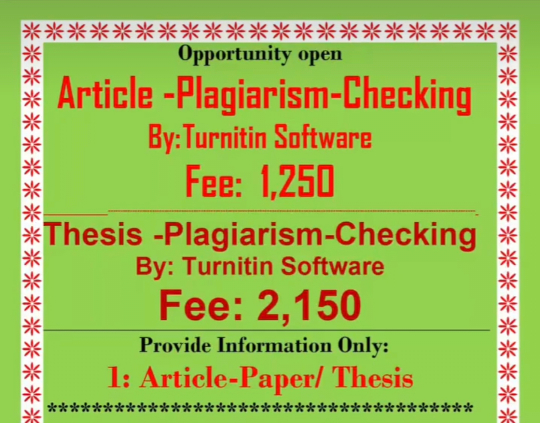
\includegraphics[width=0.5\textwidth]{img/plagiarism/Screenshot_20250328_132930_Instagram.jpg}
    \caption*{A December 10, 2024 advertisement posted on a paper mill's Instagram profile offering to submit customers' articles and theses to Turnitin for a fee.}
\end{figure}

\subsection*{Complex plagiarism: tortured phrases}

Authors who know that their work will be checked for plagiarism often try to hide it by making lots of small changes to the plagiarized text.
For instance, they may replace some words with synonyms, change the punctuation or interweave plagiarized sentences with their own.

Covering up plagiarism is often accomplished with automated paraphrasing software like those offered by \href{https://www.grammarly.com/}{Grammarly} and \href{https://quillbot.com/}{QuillBot}. These tools typically replace words and phrases in the input text with synonyms.
However, because technical works use lots of context-specific jargon, the synonyms found in a thesaurus may not be synonyms in the scientific sense.

Automated plagiarism avoidance thus creates \href{https://doi.org/10.48550/arXiv.2107.06751}{\textbf{tortured phrases}},
phrases that are devoid of scientific meaning and are often not even grammatically correct.
For instance, ``bosom peril'' is a tortured version of ``breast cancer'',
while ``computer getting to know'' is a tortured version of ``machine learning''. More instances of tortured phrases and their expected counterparts are shown in the table below.

\begin{center}
\begin{tabular}{c|c}
    Tortured phrase & Expected phrase \\ \hline\hline
     \href{https://pubpeer.com/search?q=%220.33-celebration%22}{0.33-celebration} & third party  \\ \hline
     \href{https://pubpeer.com/search?q=%22amino%20corrosive%22}{amino corrosive} & amino acid  \\ \hline
     \href{https://pubpeer.com/search?q=%22attractive%20reverberation%22}{attractive reverberation} & magnetic resonance  \\ \hline
     \href{https://pubpeer.com/search?q=%22man-made%20brainpower%22}{man-made brainpower} & artificial intelligence \\ \hline
     \href{https://pubpeer.com/search?q=%22condition%20of-workmanship%22}{condition-of-workmanship} & state-of-the-art \\ \hline
     \href{https://pubpeer.com/search?q=%22inexhaustible%20force%22%20AND%20%22renewable%20energy%22}{inexhaustible force} & renewable energy \\ \hline
     \href{https://pubpeer.com/search?q=%22bogus%20up-sides%22}{bogus up-sides} & false positives \\ \hline
     \href{https://pubpeer.com/search?q=%22message-just%22}{message-just} & text-only \\ \hline
     \href{https://pubpeer.com/search?q=%22underground%20creepy%20crawly%20state%22}{underground creepy-crawly state} & ant colony \\ \hline
     \href{https://pubpeer.com/search?q=%22vitality%20utilization%22}{vitality utilization} & energy use \\ \hline
     \href{https://pubpeer.com/search?q=%22Walk+2020%22}{Walk 2020} & March 2020 \\ \hline
\end{tabular}
\end{center}

One common variant on tortured phrases is the \href{10.1126/science.znqe1aq}{tortured acronynm}.
For instance, if the original paper contains ``Artificial Intelligence (AI)'',
a tortured version might contain ``man-made consciousness (AI)'',
retaining the acronym because the software has no concept of acronyms and thus cannot replace it.
Even proper nouns can be replaced if they are also a common noun, leading to absurdities like \href{https://pubpeer.com/publications/059D502827972226591FC5F5421221}{``Glove Romney''} replacing the name of the American politician Mitt Romney (this particular tortured phrases has also appeared \href{https://web.archive.org/web/20250322132615/https://www.amazon.com/Mitt-Romney-Biography-Book-Flexibility-ebook/dp/B0CLKZKKQG}{outside of scientific articles}).

The \href{https://www.irit.fr/~Guillaume.Cabanac/problematic-paper-screener}{Problematic Paper Screener (PPS) Tortured Phrases Detector} documents thousands of instances of tortured phrases by regularly searching the scientific literature for known tortured phrases.
Newcomers to sleuthing and post-publication peer review should consider looking through the PPS Tortured Phrases Detector for entries that have not yet been assessed by a human and follow the instructions to report the problem on PubPeer.

Tortured phrases are rarely found in isolation; if there is one tortured phrase in an article, there are likely several. When reading a paper with tortured phrases, you may encounter terms the PPS did not detect but that also look like tortured phrases. Look any suspicious phrases up in a scholarly search engine like \href{https://scholar.google.com}{Google Scholar} or \href{https://www.dimensions.ai/}{Dimensions} to see if the phrase has been used in legitimate contexts previously. If not, use the PPS Feedback tool to suggest adding your findings to the tortured phrase database. New tortured phrases can also be identified by taking established scientific terms (e.g., \href{https://doi.org/10.1007/11559573_65}{``Hahn moments''}), substituting in common synonyms and querying the resulting term in these database (\href{https://pubpeer.com/search?q=%22Hahn%20instants%22}{``Hahn instants''})

The presence of tortured phrases in an article implies 1) that parts of the article were plagiarized and 2) that the article was not genuinely peer-reviewed before publication.
No serious editor or peer reviewer would accept a paper purporting to detect ``bosom peril'' using ``man-made consciousness''.
Venues that publish such works likely publish numerous other problematic articles.

\subsection*{Complex plagiarism: translation}

Authors may plagiarize another work by translating text out of its original language and into another. This often results in non-standard grammatical structures and nonsensical sentences.

\subsection*{Detecting plagiarism and finding originals}

Simple plagiarism can often be detected by gut instinct alone. For instance, while reading a text, you may notice that:

\begin{itemize}
    \setlength\itemsep{-0.5em}
    \item the tone of the text suddenly changes;
    \item identical concepts are suddenly referred to with wildly different vocabulary; or
    \item a poorly-written manuscript suddenly switches to perfect grammar and spelling.
\end{itemize}

The best proof that text has been plagiarized is identification of the original source from which the text was plagiarized. This is much easier to accomplish for instances of simple plagiarism than for paraphrased or translated plagiarized text. For simple plagiarism, looking up one of the anomalous sentences in a search engine often brings up its source.

Finding the original text from a tortured text boils down to guessing which parts of a text have been replaced, guessing what the original words were and searching for the possible original words (see Example 2 below).

\begin{comment}
Looking for words that \emph{aren't} tortured can be useful if they are unique enough that they help narrow down the search.
\end{comment}

It is important to provide evidence that the ``original'' source predates the ``plagiarized'' version.
This can be indicate with publication or submissions dates, or other details such as the original having high-resolution versions of figures that are blurry in the copy.

\subsection*{Example 1: Simple plagiarism}

\href{https://doi.org/10.1155/2007/48242}{Cimini et al. (2007)} report on the expression of different proteins during neural stem cell differentiation. The first two paragraphs in the Introduction section of this article are nearly identical to the prior article by \href{https://doi.org/10.1016/j.plipres.2005.12.002}{Feige et al. (2006)}. This article was \href{https://doi.org/10.1155/2019/5656198}{retracted in 2019} with a retraction notice describing plagiarism and image manipulation. 

\subsection*{Example 2: Tortured phrases, original source identified}

\href{https://doi.org/10.1016/j.gltp.2021.01.002}{Alshari and Gawali (2021)} describe a technique for land-use land cover (LULC) classification. The text of the article is filled with tortured phrases. One section titled ``Hybrid approach'' begins with ``A mixture approach joins the upsides of the computerized and manual strategies to create a land cover map that is in a way that is better than if a solitary technique was available''. The section title is a hint that the original text used the word ``hybrid'' instead of ``mixture''. One might also guess that ``upsides'' should read ``advantages'' and ``computerized'' should read ``automated''. Sure enough, querying a search engine for \verb|"hybrid approach" + "advantages of the automated and manual"| returns the original text, from \href{https://www.amnh.org/content/download/74344/1391366/file/land-cover-classification-methods.pdf}{Horning (2004)}: ``A hybrid approach combines the advantages of the automated and manual methods to
produce a land cover map that is better than if just a single method was used''.

\subsection*{Example 3: Translation plagiarism, original source identified}

\href{https://doi.org/10.1111/mbe.12345}{Sadvakassova et al. (2022)} describe techniques to manage the stress of preschool students with special needs. The text, in English, is frequently nonsensical, apparently plagiarized from another work by \href{https://cyberleninka.ru/article/n/harakteristika-trevozhno-fobicheskogo-sostoyaniya-u-detey-doshkolnogo-vozrasta-s-zaderzhkoy-psihicheskogo-razvitiya-kak}{Klimova (2010)}, written in Russian. The article was retracted in 2023.

\begin{figure}[h!tbp]
    \centering
    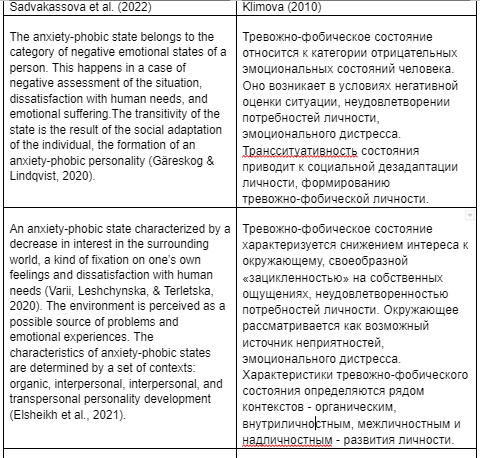
\includegraphics[width=0.8\textwidth]{img/plagiarism/image-1697289264849.png}
    \caption*{A comparison of the English text by \href{https://doi.org/10.1111/mbe.12345}{Sadvakassova et al. (2022)} to the Russian text by \href{https://cyberleninka.ru/article/n/harakteristika-trevozhno-fobicheskogo-sostoyaniya-u-detey-doshkolnogo-vozrasta-s-zaderzhkoy-psihicheskogo-razvitiya-kak}{Klimova (2010)}. Citations are added to the translated text that were not present in the original. Figure created by \href{https://pubpeer.com/publications/A6C5007F7D6DF81B20F72098A04F20\#2}{Anna Abalkina}.}
\end{figure}

\subsection*{Example 4: Duplicate publication, translated}

\href{https://doi.org/10.1007/978-3-319-51859-6_14}{Garz\'on et al. (2017)} describe a new material for greenhouses in an English-language book chapter. This chapter was \href{https://doi.org/10.1007/978-3-319-51859-6_20}{retracted in 2021} because the work was \href{https://ingenieriacivil.cedex.es/index.php/ingenieria-civil/article/view/521}{previously published} by some of the same authors in Spanish.

\pagebreak

\subsection*{Additional resources}

\begin{itemize}
    \setlength\itemsep{-0.5em}
    \item \href{https://www.ox.ac.uk/students/academic/guidance/skills/plagiarism}{Guide on plagiarism for Oxford University students}
    \item \href{https://doi.org/10.24318/cope.2019.2.2}{COPE: Plagiarism in a published article}
    \item \href{https://doi.org/10.48550/arXiv.2107.06751}{``Tortured phrases: A dubious writing style emerging in science. Evidence of critical issues affecting established journals'' (2021)}
    \item \href{https://doi.org/10.1007/978-3-030-46711-1_2}{``Disguised academic plagiarism: Translation plagiarism'' (2018)}
    \item \href{https://doi.org/10.1007/s10503-019-09481-3}{``The Pernicious Effects of Compression Plagiarism on Scholarly Argumentation'' (2019)}
    \item \href{https://ori.hhs.gov/self-plagiarism}{Self plagiarism guide from United States Department of Health and Human Service Office of Research Integrity}
    \item \href{https://textrecycling.org/}{Text Recycling Research Project}
\end{itemize}

\end{document}
\documentclass[letterpaper, 12pt]{article}

\usepackage{geometry}
 \geometry{
 letterpaper,
 total={170mm,257mm},
 left=20mm,
 top=20mm,
 bottom=20mm
 }
\usepackage{graphicx} % Required for inserting images
\usepackage{authblk}
\usepackage{amssymb}
\usepackage{lipsum}
\usepackage{float}
\usepackage{times}
\usepackage{amsmath}
\usepackage[format=plain,
            labelfont={bf,it},
            textfont=it]{caption}
\captionsetup{justification=raggedright,singlelinecheck=false}
\usepackage{ragged2e}
\usepackage{longtable}
\usepackage{comment}
\usepackage{setspace}
\usepackage{fancyhdr}
\usepackage{titlesec}
\usepackage[hyperindex,breaklinks]{hyperref}
\hypersetup{
    colorlinks=true,
    linkcolor=blue,
    filecolor=magenta,      
    urlcolor=blue
    }
% \usepackage{background} % add COSIG logo to page
\usepackage[T1]{fontenc}
\usepackage{helvet}
\renewcommand{\familydefault}{\sfdefault}
\pagenumbering{gobble}
\usepackage[skip=10pt plus1pt, indent=40pt]{parskip}

\titlespacing*{\section}
{0pt}{1.5ex plus 1ex minus .2ex}{1.3ex plus .2ex}

\renewcommand\Authfont{\fontsize{12}{14.4}\selectfont}
\renewcommand\Affilfont{\fontsize{9}{10.8}\itshape}
 
\begin{document}
\flushleft

\includegraphics[width=0.5\textwidth]{img/home/241017_final_logo_mockup.png}

\section*{Common dismissive responses to integrity concerns}
\addcontentsline{toc}{section}{Common dismissive responses to integrity concerns}
\textit{Last updated: 22 May 2025}

Authors, editors and research integrity officers sometimes respond dismissively to valid publication integrity concerns. This guide covers a handful of such responses commonly encountered by post-publication peer reviewers and provides frameworks for responding to them.

\subsection*{``We do not respond to anonymous complaints.''\newline 
``Please share your name and email address and we will send you the data.''}

Post-publication peer reviewers sometimes become targets for harassment and litigation. Researchers risk jeopardizing their careers by raising integrity issues in the publications of prominent scientists in their field. Anonymity and pseudonymity protect post-publication peer reviewers from retaliation. Many post-publication peer reviewers would likely not share their observations if they were required to publicly share their identity. For similar reasons, anonymity of peer reviewers has long been \href{https://doi.org/10.1038/6295}{accepted as standard} in pre-publication peer review pipelines. 

In their \href{https://doi.org/10.24318/cope.2019.2.25}{flowchart on responding to integrity concerns raised directly with editors}, the Committee on Publication Ethics (COPE) advises ``[sometimes] the whistleblower may prefer
to remain anonymous. It is important not to try to `out' people who wish to be anonymous.'' COPE also \href{https://doi.org/10.24318/Z9gtPzCa}{recommends} that anonymous whistleblowers ``should be treated courteously and the complaint investigated appropriately, as it would be if the complaint were from another source''.

Moreover, a peer reviewer's anonymity does not prevent authors from sharing original images or data. Instead of sending data to a single commenter over email, authors can upload data to a data sharing service like \href{https://datadryad.org/stash}{Dryad}, \href{https://figshare.com/}{figshare}, \href{https://zenodo.org/}{Zenodo} or \href{https://osf.io/}{Open Science Framework} and share a link to the dataset publicly, allowing others beyond the original commenter to access their data.

\subsection*{``You are not a scientist and are thus not qualified to review this work.''\newline``Please provide an article that you have published on this subject.''}

Publication integrity concerns should be evaluated based on the substance of the concern, not the credentials or experience of the commenter raising the concern.

\subsection*{``The images shown in this article are representative/illustrative in nature and are not actual data.''}

\href{https://doi.org/10.1007/978-1-62703-056-4_1}{Images are data}. Whether or not the images in an article are presented as representative of a larger set of experimental observations, images are present to convey information to the reader. The presence of problematic images implies that the information they convey is inaccurate and can shake readers' confidence in the veracity of other information presented in the article. 

Moreover, images provide valuable information for those looking to reproduce experiments, setting expectations for what samples should look like if the experiments are performed correctly. If these images are not faithful representations of an experimental condition, the reproducibility of the work is hindered.

\subsection*{``These images were published a long time ago, when digital image manipulation was not possible.''\newline``These images were collected on analog technology and thus could not have been manipulated.''}

Digital manipulation of images has been regarded as a means for distortion of data presented in scientific articles since \href{https://doi.org/10.1002/(SICI)1096-9896(199711)183:3%3C253::AID-PATH927%3E3.0.CO;2-P}{as early as 1997} (see additional commentary on the topic \href{https://doi.org/10.1083/jcb.200406019}{published in 2004}).

Outside of the scientific literature, manipulation of photographs is \href{https://iisjoa.org/sites/default/files/iisjoa/2017/PDF/11.%20Jitendra%20Sharma%20&%20Rohita%20Sharma.pdf}{as old as photography itself} (consider the practice of \href{https://en.wikipedia.org/wiki/Spirit_photography}{spirit photography} or \href{https://en.wikipedia.org/wiki/Exaggeration_postcard}{tall-tale postcards}). Retractions have even been issued for apparent image manipulation in scientific articles published well before digital image manipulation software became widely available. For instance, \href{https://doi.org/10.1128/jvi.56.1.284-292.1985}{Fusco et al. (1985)} was \href{https://doi.org/10.1128/jvi.02169-17}{retracted in 2018} for apparent manipulation of images of \href{https://doi.org/10.1093/nar/7.6.1541}{RNA dot blots}.

\begin{figure}[h!tbp]
    \centering
    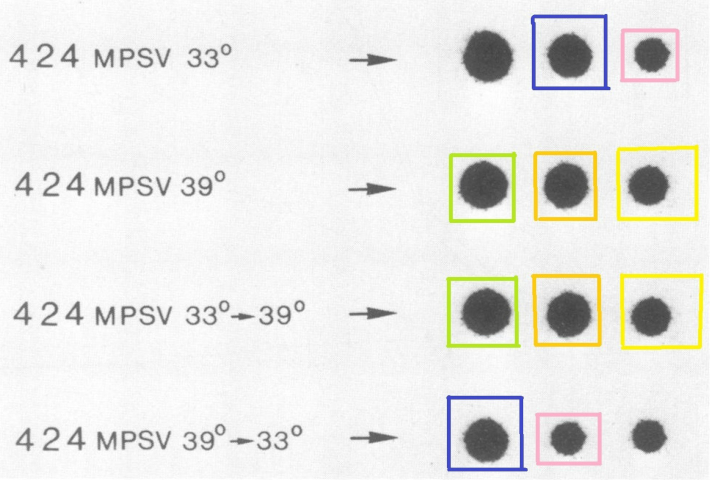
\includegraphics[width=0.8\textwidth]{img/responses/imgur-ESa5N4V_scaled.jpg}
    \caption*{\href{https://doi.org/10.1128/jvi.56.1.284-292.1985}{Fusco et al. (1985)} reports on RNA quantification experiments with dot blot images that have apparently been manipulated. Colored boxes indicate portions of the image that are identical to one another. Adapted from Figure 8 of Fusco et al. by \href{https://pubpeer.com/publications/67130CFDA6D3D4F59D463598ACE835\#3}{an anonymous PubPeer commenter}.}
\end{figure}

\pagebreak

\subsection*{``This comment concerns one image among dozens with no issues in this article.''}

When one image or piece of data in one part of an article has concerning irregularities, it is reasonable for readers to have doubts about other data reported in the article.

Consider a hypothetical instance where there are extensive internal duplications in a published image suggestive of deliberate manipulation. Readers cannot know who among the authors was responsible for this manipulation, their motivations, nor what other data in the article may have been manipulated. When any signs of manipulation are present, readers are left wondering whether there is more instances of manipulation that are impossible to discover by examining the published article alone.

\subsection*{``We did not use tortured phrases, just alternative scientific terminology.''}

There are instances where using scientific nomenclature that departs from more commonly-used language is acceptable. Using \href{https://pubpeer.com/search?q=%22bosom+disease%22}{``bosom disease''} in place of ``breast cancer'' is not one of these instances.

See the section on tortured phrases in the \href{https://osf.io/ntcb4}{COSIG guide on textual plagiarism}.

\subsection*{``There are no duplicated regions in the image in question; these regions only appear similar because of structural similarities in the sample.''}

There is expected to be some similarity in appearance between particles in a sample, cells in culture, physiological structures in a tissue sample, bands in a Western blot, etc. However, large regions of an image actually depicting different objects are unlikely to be identical down to the pixel. If authors believe that similarities between images or regions of an image are in fact due to chance alone, they can alleviate concerns by providing the original, high-resolution images corresponding to those shown in the article.

\begin{figure}[h!tbp]
    \centering
    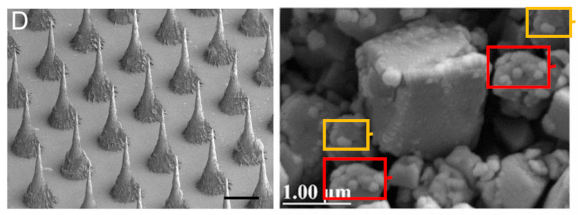
\includegraphics[width=\textwidth]{img/responses/yu_vs_mohaghegh_0.png}
    \caption*{\href{https://doi.org/10.1073/pnas.1505405112}{Yu et al. (2015)} show a scanning electron microscope (SEM) image (left, adapted from Figure 4D) of a microneedle array cast from a precisely-fabricated silicon mold. Each microneedle is designed to have the same shape as the next. However, no two microneedles appear exactly alike. On the other hand, \href{https://doi.org/10.1007/s10853-015-9003-3}{Mohaghegh et al. (2015)} report synthesizing crystal nanoparticles by precipitation from solution, for which it would be impossible to exactly control the shape of the synthesized product. However, one of the images of these nanoparticles shown in the article (right, adapted from Figure 3A by \href{https://pubpeer.com/publications/7BE7C2A93C385F700F1C6B5BC90294\#1}{Reese Richardson on PubPeer}) contains large regions that are identical to one another (highlighted by colored boxes). It is highly unlikely that any two nanoparticles in this sample actually appeared this similar to one another.}
\end{figure}

\end{document}

\documentclass[letterpaper, 12pt]{article}

\usepackage{geometry}
 \geometry{
 letterpaper,
 total={170mm,257mm},
 left=20mm,
 top=20mm,
 bottom=20mm
 }
\usepackage{graphicx} % Required for inserting images
\usepackage{authblk}
\usepackage{amssymb}
\usepackage{lipsum}
\usepackage{float}
\usepackage{times}
\usepackage{amsmath}
\usepackage[format=plain,
            labelfont={bf,it},
            textfont=it]{caption}
\captionsetup{justification=raggedright,singlelinecheck=false}
\usepackage{ragged2e}
\usepackage{longtable}
\usepackage{comment}
\usepackage{setspace}
\usepackage{fancyhdr}
\usepackage{titlesec}
\usepackage[hyperindex,breaklinks]{hyperref}
\hypersetup{
    colorlinks=true,
    linkcolor=blue,
    filecolor=magenta,      
    urlcolor=blue
    }
% \usepackage{background} % add COSIG logo to page
\usepackage[T1]{fontenc}
\usepackage{helvet}
\renewcommand{\familydefault}{\sfdefault}
\pagenumbering{gobble}
\usepackage[skip=10pt plus1pt, indent=40pt]{parskip}

\titlespacing*{\section}
{0pt}{1.5ex plus 1ex minus .2ex}{1.3ex plus .2ex}

\renewcommand\Authfont{\fontsize{12}{14.4}\selectfont}
\renewcommand\Affilfont{\fontsize{9}{10.8}\itshape}
 
\begin{document}
\flushleft

\includegraphics[width=0.5\textwidth]{img/home/241017_final_logo_mockup.png}

\section*{Image duplication}
\addcontentsline{toc}{section}{Image duplication}
\textit{Last updated: 22 May 2025}

Image duplication is one of the most frequently spotted integrity issues in scientific publications. This term is generally used to describe instances where two images (or parts of an image) are supposed to represent different things but are actually identical.

\href{https://doi.org/10.1128/mbio.00809-16}{Bik et al. (2016)} established a typology of image duplications, summarized below. Additional examples are provided in the external resources listed at the end of this guide.

\subsection*{Type I: Simple duplication}

This describes when the same image has been used multiple times to represent different experiments or samples. Sometimes, the same image is used multiple times in an article to represent the same experiment, which is usually not considered problematic.

\subsection*{Type II: Duplication with repositioning}

This describes when the same image has been used multiple times to represent different experiments or samples, but in one or more of these instances the image has been cropped, rotated, flipped or otherwise repositioned.

\subsection*{Type III: Duplication with alteration} 

This describes when the same image has been used multiple times, but one or more instances of this image have been altered relative to the others via the addition or subtraction of certain features. This category also covers duplicated regions within a single image shown in 
an article.

Among the above categories, Type I is considered the least severe (and most likely to be the result of an error during figure preparation) while Type III is considered the most severe (and most likely to be the result of deliberate image manipulation). 

As noted by \href{https://doi.org/10.1017/jme.2025.32}{Brookes (2025)}, Type I, II and III duplications can occur within an article as well as between different articles. In cases where an image has been re-used in multiple articles, it is problematic when these images are supposed to represent different experiments or have not been properly attributed to the original authors that collected or published the image.

\subsection*{Tools for detecting duplications}

Several software tools have been developed to help the user find image duplications within or between figures. These are described separately in COSIG's entry \href{https://osf.io/g23pf}{on software for image forensics}.

\subsection*{Common false positives}

There is a difference between appropriate and inappropriate image duplications. Not all duplications that might be spotted by eye or flagged by image forensics software might be inappropriate. For example, image panels representing control samples (e.g., loading controls in Western blots, untreated mice, etc) might be used multiple times within the same article. If those images represent the same experimental conditions, this is not considered a problem. 

Review articles will often republish images used in previous articles. This is only problematic if the review article misrepresents the image being used or does not properly attribute it to its original source.

Many articles will include images from publicly-available datasets (e.g., the \href{https://www.cs.toronto.edu/~kriz/cifar.html}{CIFAR datasets} or histopathology images from the \href{https://www.proteinatlas.org/}{Human Protein Atlas}). Again, as long as these images are properly attributed and not misrepresented, this is not problematic.

The different channels in \href{https://en.wikipedia.org/wiki/Fluorescence_microscope}{fluorescence microscopy} images are often displayed in separate panels alongside a panel where all channels are merged. Although it may appear that these images are inappropriately duplicated, they in fact represent the same data and presenting images in this way is not problematic.

\subsection*{Annotating image duplications}

When reporting observations of image duplications on PubPeer or to journal editors, it is often useful to illustrate exactly which images / regions are apparently duplicated. This is often accomplished by overlaying colored boxes on the image (as shown in the examples below) where each color corresponds to a different set of shared image features. These annotations are usually performed in software like \href{https://www.microsoft.com/en-us/windows/paint}{Microsoft Paint}, \href{https://www.gimp.org/}{GIMP}, \href{https://www.microsoft.com/en-us/microsoft-365/powerpoint}{Microsoft PowerPoint} or \href{https://support.apple.com/guide/preview/welcome/mac}{Preview (for Mac)}. 

If annotating an article with many apparent duplications, you may find yourself running out of unique colors to use. Using too many colors can make annotations difficult to interpret. Strive for readability when annotating images -- it is often useful to show the original image alongside the annotated image.

For Type II and Type III duplications that involve rotation or flipping, it is often useful to attach a small symbol to each of the boxes to make it more apparent what transformation occurred, such as a small diagonal line on the side of the box. 

A PowerPoint template containing several pre-made boxes and symbols for annotating images is \href{https://osf.io/w3epj}{available here}.
\begin{figure}[h!tbp]
    \centering
    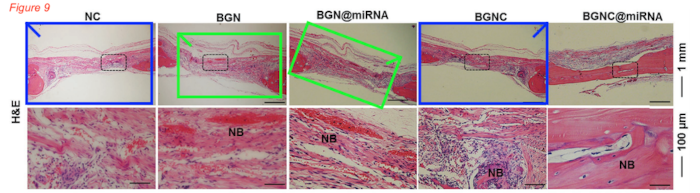
\includegraphics[width=\textwidth]{img/image_duplication/xue_fig_9_small.png}
    \caption*{An annotated figure showing Type II image duplications between panels. Note that a small diagonal line is affixed to each of these boxes to make their relative rotation and flipping more apparent. Adapted from Figure 9 of \href{https://doi.org/10.1002/adhm.201700630}{Xue et al. (2017)} by \href{https://pubpeer.com/publications/C47278BACD8304A719E502DF7041A5\#1}{Elisabeth Bik on PubPeer}.}
\end{figure}

\begin{figure}[h!tbp]
    \centering
    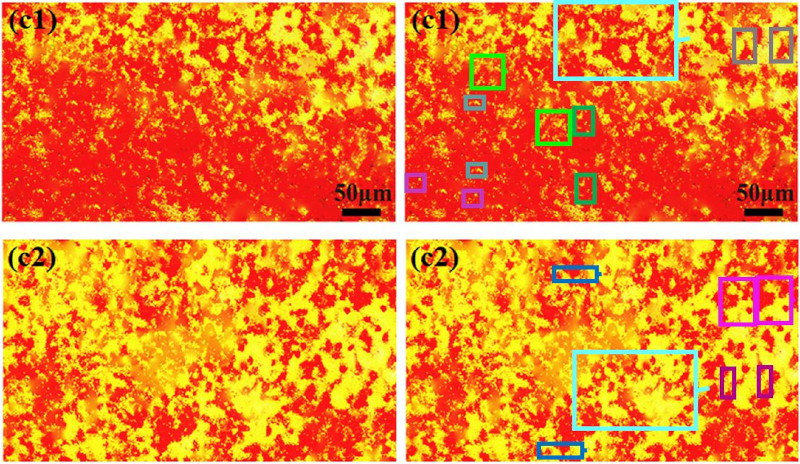
\includegraphics[width=\textwidth]{img/image_duplication/Bakhsheshi-Rad_annotation.JPG}
    \caption*{An original set of published images of cell culture (left) versus an annotated version of these images showing regions of unusually high similarity (right). Adapted from Figure 4C of \href{https://doi.org/10.1016/j.polymertesting.2019.106298}{Bakhsheshi-Rad et al. (2020)} by \href{https://pubpeer.com/publications/60A225978670EFD93446CAC5696F7F\#1}{Reese Richardson on PubPeer}. This represents a Type III duplication. Note also that some of the boxed regions (e.g., the cyan boxes) are unusually similar, but not exactly identical to one another.}
\end{figure}

\subsection*{Example 1: Type I duplication}

\href{https://doi.org/10.1172/JCI66764}{Morrison et al. (2013)} describe experiments in breast cancer cell cultures with visible light microscopy images. However, two of the images used in Figure 4 to describe different experimental conditions are identical.

\begin{figure}[h!tbp]
    \centering
    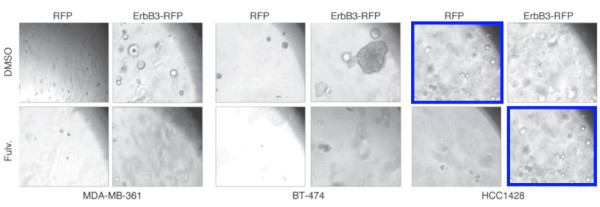
\includegraphics[width=\textwidth]{img/image_duplication/image-1744937326665.jpg}
    \caption*{Two panels representing different experimental conditions (one representing RFP-expressing cells treated with DMSO and one representing ErbB3-RFP-expressing cells treated with fulvestrant) are identical, as indicated by blue boxes. Adapted from Figure 4 of \href{https://doi.org/10.1172/JCI66764}{Morrison et al. (2013)} by \href{https://pubpeer.com/publications/2768B5B42E7338AB72D4CFE660596A\#1}{Sholto David on PubPeer}.}
\end{figure}

\pagebreak

\subsection*{Example 2: Type II duplication}

Morrison et al. also provide histopathological images of implanted tumors. One image shown in Figure 2 and one image shown in Figure 7 show the same sample despite representing different treatments. The image shown in Figure 2 is cropped differently than that shown in Figure 7.

\begin{figure}[h!tbp]
    \centering
    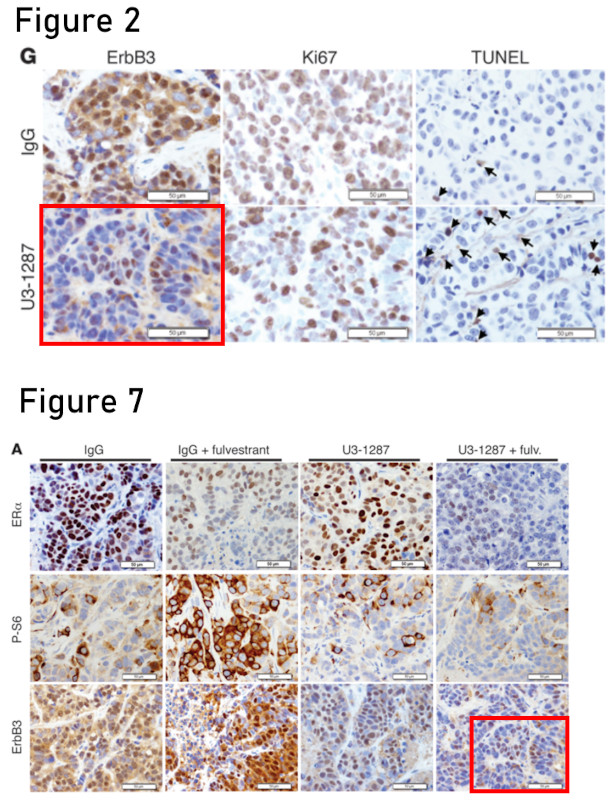
\includegraphics[width=0.7\textwidth]{img/image_duplication/image-1744937642757.jpg}
    \caption*{Two panels representing different experimental conditions (one representing tumor-bearing mice treated with antibody U3-1287 and one representing tumor-bearing mice treated with antibody U3-1287 and fulvestrant) show the same sample. The two images are cropped differently. The region the two images share in common is highlighted with red boxes. Adapted from \href{https://doi.org/10.1172/JCI66764}{Morrison et al. (2013)} by \href{https://pubpeer.com/publications/2768B5B42E7338AB72D4CFE660596A\#2}{Sholto David on PubPeer}.}
\end{figure}

\subsection*{Example 3: Type III duplication}

\href{https://doi.org/10.1007/s10853-015-9003-3}{Mohaghegh et al. (2015)} report synthesizing crystal nanoparticles. One of the scanning electron microscope (SEM) images they show of their synthesized particles contain regions that are exactly identical to one another. This is very unlikely to have occured by chance.

\begin{figure}[h!tbp]
    \centering
    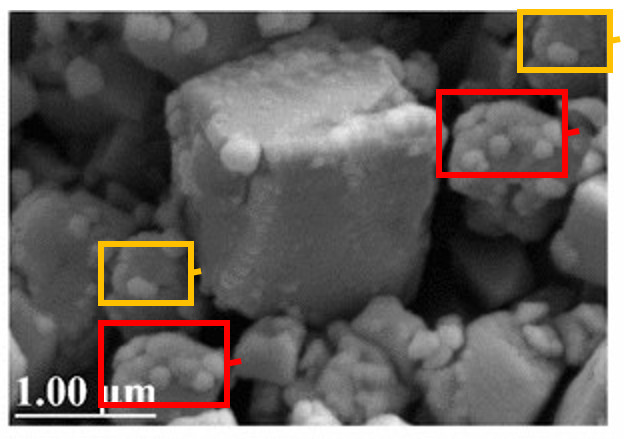
\includegraphics[width=\textwidth]{img/image_duplication/image-1741643734642.jpg}
    \caption*{In this SEM image of nanoparticles, the colored boxes shown here enclose regions that are exactly identical to one another. Adapted from Figure 3A of \href{https://doi.org/10.1007/s10853-015-9003-3}{Mohaghegh et al. (2015)} by \href{https://pubpeer.com/publications/7BE7C2A93C385F700F1C6B5BC90294\#1}{Reese Richardson on PubPeer}.}
\end{figure}

\pagebreak

\subsection*{Example 4: Type II duplication between articles}

\href{https://doi.org/10.3390/ph16070925}{Badr et al. (2023)} reuses a scanning electron microscope image previously used by \href{https://doi.org/10.2147/ijn.s77731}{Kurakala et al. (2015)} to represent a different material. In Badr et al., the image has been rotated 180 degrees and cropped. The metadata banners included in the image are inconsistent with one another and show wildly different scale bars. Because the metadata banners appear to have been altered, this could also be classified as a Type III duplication.

\begin{figure}[h!tbp]
    \centering
    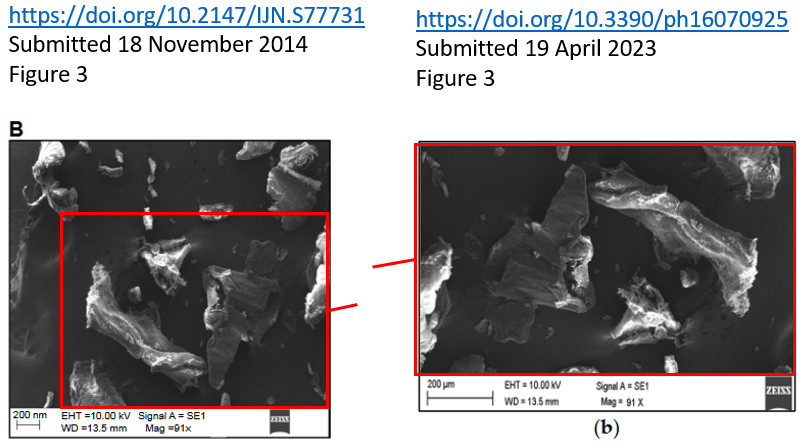
\includegraphics[width=\textwidth]{img/image_duplication/image-1741998932949.jpg}
    \caption*{\href{https://doi.org/10.3390/ph16070925}{Badr et al. (2023)} uses a scanning electron microscope image to represent itopride hydrochloride. The same image was previously used by \href{https://doi.org/10.2147/ijn.s77731}{Kurakala et al. (2015)} to represent chitosan. Note that the two images are accompanied by inconsistent scale bars (the scale bar in the Kurakala et al. image suggests particles one thousand times larger than that shown by Badr et al.). The image shown by Badr et al. has been cropped and rotated 180 degrees relative to the image shown by Kurakala et al. The shared region is shown with red boxes. Note that a small diagonal line is affixed to each of these boxes to make their relative rotation more apparent. Adapted from Badr et al. and Kurakala et al. by \href{https://pubpeer.com/publications/30DDCFCF4925C0DD401AA9810AC0A3}{Reese Richardson on PubPeer}.}
\end{figure}

\pagebreak

\subsection*{Example 5: Type III duplication}

\href{https://doi.org/10.1371/journal.pone.0058855}{Zhou et al. (2013)} report on protein expression in one experiment using Western blots. In one of their Western blots, two of the lanes shown representing particular time points appear identical to the adjacent two lanes representing later time points. This article was \href{https://doi.org/10.1371/journal.pone.0322907}{retracted in 2025} for image integrity concerns and use of \href{https://osf.io/d7we5}{contaminated cell lines}.

\begin{figure}[h!tbp]
    \centering
    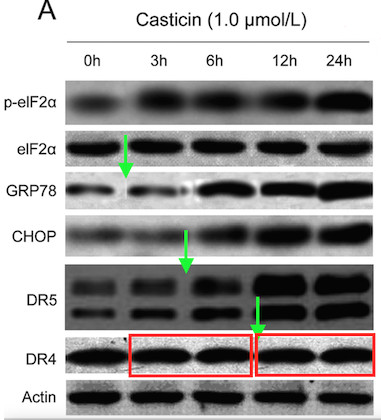
\includegraphics[width=0.7\textwidth]{img/image_duplication/image-1583362705327.jpg}
    \caption*{The 3h and 6h lanes of the DR4 panel of this series of Western blot images are identical to the 12h and 24h lanes, as shown with red boxes. Vertical green arrows indicate sharp vertical transitions between lanes, representing potential instances where images have been spliced. Adapted from Figure 6A of \href{https://doi.org/10.1371/journal.pone.0058855}{Zhou et al. (2013)} by \href{https://pubpeer.com/publications/2596C5A7287C83AFB4518CEF8AF7B4\#1}{Elisabeth Bik on PubPeer}.}
\end{figure}

\pagebreak

\subsection*{Example 6: False positive, merged fluorescence microscopy image, no problematic image duplication}

\href{https://doi.org/10.1371/journal.pone.0083018}{Lepore et al. (2013)} use fluorescence microscopy to visualize protein localization within individual cells. As is conventional for this type of data, they represent their fluorescence microscopy images as separate images for each channel (green and blue) as well as an image that merges both channels. The merged image appears similar to the images with separated channels because it represents the exact same data. Thus, there is no problematic image duplication here.

\begin{figure}[h!tbp]
    \centering
    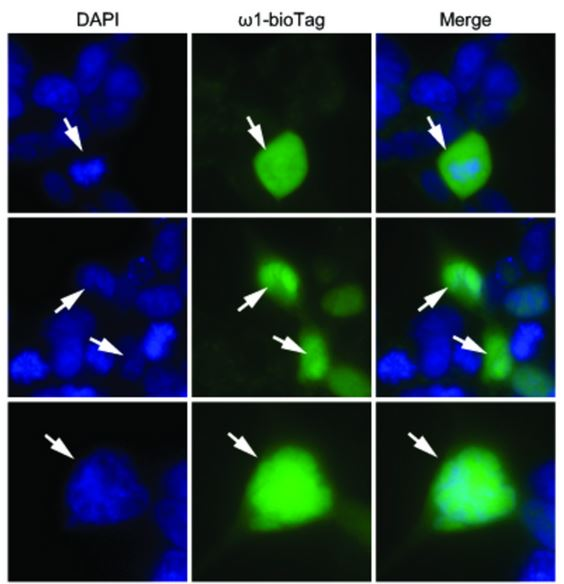
\includegraphics[width=0.7\textwidth]{img/image_duplication/merge.JPG}
    \caption*{Fluorescence microscopy images where each row contains an image showing the DAPI (blue, left) channel, the $\omega$1-bioTag (green, center) channel and a merged channel (right). Adapted from Figure 6D of \href{https://doi.org/10.1371/journal.pone.0083018}{Lepore et al. (2013)}.}
\end{figure}

\pagebreak

\subsection*{Example 7: False positive, re-used control Western blot panel}

\href{https://doi.org/10.1038/ni.1876}{Yang et al. (2010)} report on chromatin immunoprecipitation (ChIP) experiments using Western blots. In Figure 6D, they compare three different outputs to the same set of control bands, re-using the image of the control bands three times. This may appear like a problematic Type I image duplication, but this image is being re-used to represent the same experiments.

\begin{figure}[h!tbp]
    \centering
    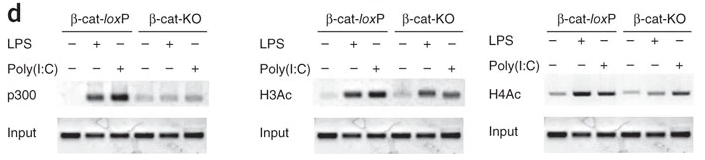
\includegraphics[width=\textwidth]{img/image_duplication/yang_fig_6d.png}
    \caption*{Note that the ``Input'' band images shown for each subpanel are identical. Because these are supposed to represent the same experiment, this is not a problem. However, for this kind of figure, the p300, H3Ac and H4Ac blot panels would usually be displayed together in the same stacked panel. Adapted from Figure 6D of \href{https://doi.org/10.1038/ni.1876}{Yang et al. (2010)}.}
\end{figure}

\subsection*{Additional resources}

\begin{itemize}
    \setlength\itemsep{-0.5em}
    \item \href{https://doi.org/10.1128/mbio.00809-16}{``The Prevalence of Inappropriate Image Duplication in Biomedical Research Publications'' (2016)}
    \item \href{https://scienceintegritydigest.com/2020/01/08/types-of-image-duplications/}{``Types of image duplications: the palm trees'' (2020)}
    \item \href{https://doi.org/10.1017/jme.2025.32}{``Misconduct Detection — Evolving Methods \& Lessons from 15 Years of Scientific Image Sleuthing'' (2025)}
    \item \href{https://osf.io/g23pf}{COSIG: Software for image forensics}
\end{itemize}

\end{document}
\documentclass[letterpaper, 12pt]{article}

\usepackage{geometry}
 \geometry{
 letterpaper,
 total={170mm,257mm},
 left=20mm,
 top=20mm,
 bottom=20mm
 }
\usepackage{graphicx} % Required for inserting images
\usepackage{authblk}
\usepackage{amssymb}
\usepackage{lipsum}
\usepackage{float}
\usepackage{times}
\usepackage{amsmath}
\usepackage[format=plain,
            labelfont={bf,it},
            textfont=it]{caption}
\captionsetup{justification=raggedright,singlelinecheck=false}
\usepackage{ragged2e}
\usepackage{longtable}
\usepackage{comment}
\usepackage{setspace}
\usepackage{fancyhdr}
\usepackage{titlesec}
\usepackage[hyperindex,breaklinks]{hyperref}
\hypersetup{
    colorlinks=true,
    linkcolor=blue,
    filecolor=magenta,      
    urlcolor=blue
    }
% \usepackage{background} % add COSIG logo to page
\usepackage[T1]{fontenc}
\usepackage{helvet}
\renewcommand{\familydefault}{\sfdefault}
\pagenumbering{gobble}
\usepackage[skip=10pt plus1pt, indent=40pt]{parskip}

\titlespacing*{\section}
{0pt}{1.5ex plus 1ex minus .2ex}{1.3ex plus .2ex}

\renewcommand\Authfont{\fontsize{12}{14.4}\selectfont}
\renewcommand\Affilfont{\fontsize{9}{10.8}\itshape}
 
\begin{document}
\flushleft

\includegraphics[width=0.5\textwidth]{img/home/241017_final_logo_mockup.png}

\section*{Example title}
\addcontentsline{toc}{section}{Example title}
\textit{Last updated: X Month 20XX}

This is a template for new guides to be added to COSIG.

\subsection*{Example section heading}

\begin{figure}[h!tbp]
    \centering
    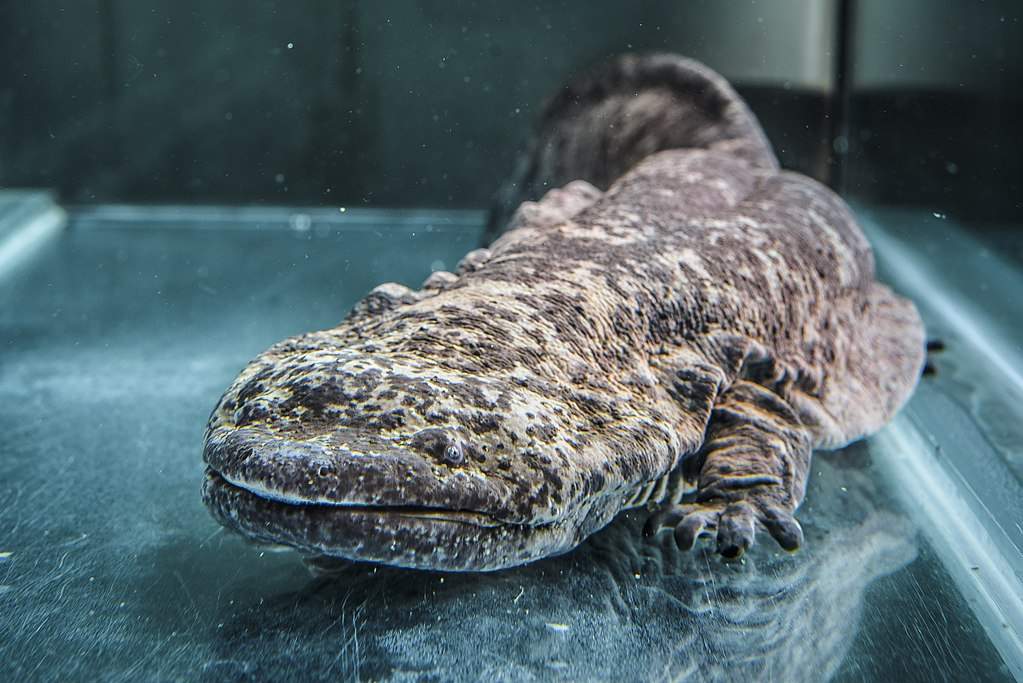
\includegraphics[width=0.8\textwidth]{img/home/chinese_giant_salamander.jpg}
    \caption*{Example of a figure. Image available \href{https://commons.wikimedia.org/wiki/File:Velemlok_\%C4\%8D\%C3\%ADnsk\%C3\%BD_zoo_praha_1.jpg}{here}.}
\end{figure}

\begin{itemize}
    \setlength\itemsep{-0.5em}
    \item bullet
    \item point
    \item list
\end{itemize}

\begin{enumerate}
    \setlength\itemsep{-0.5em}
    \item numbered
    \item list
\end{enumerate}

\pagebreak

\begin{center}
\begin{tabular}{|p{3.0cm}|p{3.0cm}|p{3.0cm}|}
\hline
     A & B & C\\ \hline\hline
     1 & 2 & 3\\\hline
     $\alpha$ & $\beta$ & $\gamma$\\ \hline
\end{tabular}
\end{center}

\begin{center}
\begin{tabular}{l|ccc}
& \multicolumn{3}{c}{predicted class} \\
true class & lemon & orange & tangerine \\
\hline
lemon & 1 & 1 & 0\\
orange & 0 & 1 & 2\\
tangerine & 0 & 0 & 1\\
\end{tabular}
\end{center}

If there is a large block of quoted text, use:

\begin{quote}
    \textit{Note that this text is in italics!}
\end{quote}

When linking out to articles using \verb|\href|, try to use the DOI instead of a link to the publisher site or PubMed page.

\end{document}
\documentclass[letterpaper, 12pt]{article}

\usepackage{geometry}
 \geometry{
 letterpaper,
 total={170mm,257mm},
 left=20mm,
 top=20mm,
 bottom=20mm
 }
\usepackage{graphicx} % Required for inserting images
\usepackage{authblk}
\usepackage{amssymb}
\usepackage{lipsum}
\usepackage{float}
\usepackage{times}
\usepackage{amsmath}
\usepackage[format=plain,
            labelfont={bf,it},
            textfont=it]{caption}
\captionsetup{justification=raggedright,singlelinecheck=false}
\usepackage{ragged2e}
\usepackage{longtable}
\usepackage{comment}
\usepackage{setspace}
\usepackage{fancyhdr}
\usepackage{titlesec}
\usepackage[hyperindex,breaklinks]{hyperref}
\hypersetup{
    colorlinks=true,
    linkcolor=blue,
    filecolor=magenta,      
    urlcolor=blue,
    pdftitle={Overleaf Example},
    pdfpagemode=FullScreen,
    }
% \usepackage{background} % add COSIG logo to page
\usepackage[T1]{fontenc}
\usepackage{helvet}
\renewcommand{\familydefault}{\sfdefault}
\pagenumbering{gobble}
\usepackage[skip=10pt plus1pt, indent=40pt]{parskip}

\begin{comment}
\backgroundsetup{
   scale=1,
   angle=0,
   opacity=1,
   color=black,
   contents={\begin{tikzpicture}[remember picture, overlay]
      \node at ([xshift=3cm,yshift=1cm] current page.south west)
            {
\includegraphics[width = 5cm]{img/home/241017_final_logo_mockup.png}}; %<- change the name of image
     \end{tikzpicture}}
 }
\end{comment}

\titlespacing*{\section}
{0pt}{1.5ex plus 1ex minus .2ex}{1.3ex plus .2ex}

\renewcommand\Authfont{\fontsize{12}{14.4}\selectfont}
\renewcommand\Affilfont{\fontsize{9}{10.8}\itshape}
 
\begin{document}
\flushleft

\includegraphics[width=0.5\textwidth]{img/home/241017_final_logo_mockup.png}

\section*{Software for image forensics}
\textit{Last updated: 7 February 2025}

Publication integrity issues often arise from image integrity issues. Performing image forensics is often very useful for taking part in post-publication peer review, especially in fields that frequently use images in scientific articles (e.g., biomedicine).

While many image integrity issues can be spotted by eye, it is often easier and more efficient to use software to automatically spot issues or make issues more visible to readers. This guide is a catalog of tools and software that are commonly used by sleuths.

Here are some factors to consider when using these tools:

\begin{itemize}
    \setlength\itemsep{-0.5em}
    \item \textbf{There can be false positives.} A tool may flag image features that, upon closer manual examination, do not actually indicate any image integrity issues.
    \item \textbf{There can be false negatives.} A tool may not flag image features that are indicative of image integrity issues. For instance, software for detecting image duplications within a figure may miss some duplications that are visible by eye.
    \item \textbf{Tools may not examine all data types.} There can be entire categories of data (including image data) that have been explicitly excluded by the programmers of a tool because they are not yet comfortable with the sensitivity/specificity of their tool for that data type.
    \item \textbf{Analysis may not be reproducible.} Some of these services and software are updated frequently and the current version of a tool may not yield the same results as a previous version.
    \item \textbf{Analysis of the same images in a different format may yield different results.} For example, if one uploads an entire PDF to a duplication detection tool, the tool may yield different results than if individual images are uploaded, even if the individual images and those in the PDF appear identical by eye. Figures in published articles will often be available in multiple resolutions, which can yield differing results. When performing image forensics, it is always preferable to work with the original, full-resolution, uncropped images provided by a study's authors.
    \item \textbf{Tweaking parameters can yield differing results.} Some tools have sensitivity settings that can be changed by the user. Changing these setting may produce different results for the same images.
    \item \textbf{Different tools do different things.} Not every tool described here has the same functionality or use cases as another tool. Another person without access to your tool of choice may not be able to reproduce your analysis.
\end{itemize}

\pagebreak
\subsection*{Software/tools commonly used for image forensics in post-publication peer review:}

\begin{itemize}
    \setlength\itemsep{-0.5em}
    \item \textbf{\href{https://www.adobe.com/products/photoshop.html}{Adobe Photoshop} (subscription-based)}. Photoshop is an image manipulation software that allows users to adjust color levels, adjust brightness and contrast, overlay images and annotate figures among myriad other features. The United States Department of Health and Human Service Office of Research Integrity provides \href{https://ori.hhs.gov/advanced-forensic-actions}{some toolkits} for image forensics with Photoshop.
    \item \textbf{\href{https://www.gimp.org/}{GIMP (the GNU Image Manipulation Program)} (free to use and open-source)}. GIMP is a image manipulation software with most of the same features and functionality as Photoshop but is free to use (and modify).
    \item \textbf{\href{https://imagetwin.ai/}{Imagetwin} (subscription-based)}. Imagetwin is a browser-based service that allows users to upload article PDFs and individual images, which it will then compare against a large database of published images to see if parts of any of the uploaded images have been used previously. It also detects within-document image duplication and splicing of certain images (e.g., \href{https://en.wikipedia.org/wiki/Western_blot}{Western blots}). Users can control the sensitivity of detection on the Results page of a scan.
    \item \textbf{\href{https://www.proofig.com/}{Proofig} (subscription-based)}. Proofig is a browser-based service that allows users to upload article PDFs and individual images, which it will then compare against a large database of published images to see if parts of any of the uploaded images have been used previously. It also detects within-document image duplication.
    \item \textbf{\href{https://github.com/GuidoBartoli/sherloq}{Sherloq } (free to use and open-source)}. Sherloq is a software environment for image forensics that can be installed on Linux and Windows. Users can perform various image transformations that make manipulation more apparent (such as visualizing \href{https://en.wikipedia.org/wiki/Image_gradient}{luminence gradient}) as well as inspect image metadata.
    \item \textbf{\href{https://29a.ch/photo-forensics/}{Forensically} (free to use)}. Forensically is a browser-based service that offers several tools for image forensics, such as clone detection and levels adjustment.
    \item \textbf{\href{https://fotoforensics.com/}{FotoForensics} (free to use)}. FotoForensics is a browser-based service that offers several tools for image forensics, such as \href{https://en.wikipedia.org/wiki/Error_level_analysis}{error level analysis} and metadata inspection.
    \item \textbf{\href{https://www.figcheck.com/imagecheck}{Figcheck} (subscription-based, limited free use)}. Figcheck is a browser-based service that detects within-document image duplication. Each user is limited to uploading 10 images a day.
    \item \textbf{\href{https://sholtodavid.pythonanywhere.com/}{Image Duplication Check (Sholto David)} (free to use)}. This is a browser-based application that allows the user to upload a PDF and scan for within-document image duplication. 
    \item \textbf{\href{https://www.google.com/?olud=}{Google Lens} (free to use)}. Google Lens is an extension of the Google search engine that allows users to upload an image and finding matching and visually-similar images across the web.
\end{itemize}

\end{document}
\documentclass[letterpaper, 12pt]{article}

\usepackage{geometry}
 \geometry{
 letterpaper,
 total={170mm,257mm},
 left=20mm,
 top=20mm,
 bottom=20mm
 }
\usepackage{graphicx} % Required for inserting images
\usepackage{authblk}
\usepackage{amssymb}
\usepackage{lipsum}
\usepackage{float}
\usepackage{times}
\usepackage[format=plain,
            labelfont={bf,it},
            textfont=it]{caption}
\captionsetup{justification=raggedright,singlelinecheck=false}
\usepackage{ragged2e}
\usepackage{longtable}
\usepackage{comment}
\usepackage{setspace}
\usepackage{fancyhdr}
\usepackage{titlesec}
\usepackage[hyperindex,breaklinks]{hyperref}
\hypersetup{
    colorlinks=true,
    linkcolor=blue,
    filecolor=magenta,      
    urlcolor=blue,
    pdftitle={Overleaf Example},
    pdfpagemode=FullScreen,
    }
% \usepackage{background} % add COSIG logo to page
\usepackage[T1]{fontenc}
\usepackage{helvet}
\renewcommand{\familydefault}{\sfdefault}
\pagenumbering{gobble}
\usepackage[skip=10pt plus1pt, indent=40pt]{parskip}

\begin{comment}
\backgroundsetup{
   scale=1,
   angle=0,
   opacity=1,
   color=black,
   contents={\begin{tikzpicture}[remember picture, overlay]
      \node at ([xshift=3cm,yshift=1cm] current page.south west)
            {
\includegraphics[width = 5cm]{img/home/241017_final_logo_mockup.png}}; %<- change the name of image
     \end{tikzpicture}}
 }
\end{comment}

\titlespacing*{\section}
{0pt}{1.5ex plus 1ex minus .2ex}{1.3ex plus .2ex}

\renewcommand\Authfont{\fontsize{12}{14.4}\selectfont}
\renewcommand\Affilfont{\fontsize{9}{10.8}\itshape}
 
\begin{document}
\flushleft

\includegraphics[width=0.5\textwidth]{img/home/241017_final_logo_mockup.png}

\section*{Extracting vector graphics from a PDF}
\textit{Last updated: 5 February 2025}

It is often difficult to tell if two line graphs have shared features from a published figure alone. While the webpage of a scientific article invariable displays these images in raster format (i.e. pixel-based), the PDF version of the article may actually display these images in vector format, meaning that the features of the figure can be more easily magnified and compared.

An easy way to check if a figure in the PDF of a scientific article is in raster format or vector format is to try highlighting the text in the figure with your cursor (e.g. the text that labels the axes of the graph). If the text within the figure can be highlighted, the image is probably in vector format. Consider \href{https://doi.org/10.1007/s12182-020-00439-9}{this article}, for which the figures in the PDF are in vector format, and \href{https://doi.org/10.1016/j.est.2023.109227}{this article}, for which the images in the PDF are in raster format.

\begin{figure}[h!tbp]
    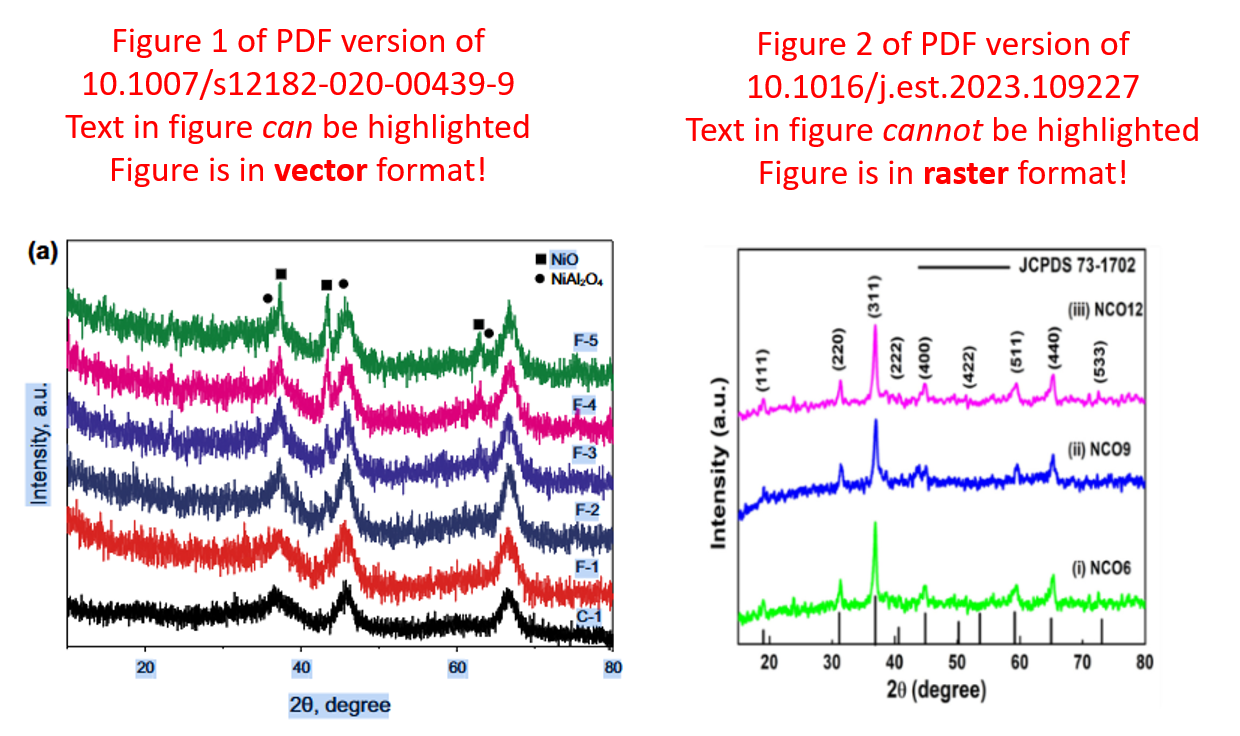
\includegraphics[width=\textwidth]{img/vector/vector_vs_raster.PNG}
    \caption*{ The figure on the left is embedded within its PDF in vector format, whereas the image on the right is embedded within its PDF in raster format.}
\end{figure}

Vector graphics can be isolated in any vector graphics editor like \href{https://www.adobe.com/products/illustrator.html}{Adobe Illustrator} or its free, open-source alternative \href{https://inkscape.org/}{Inkscape}. We'll use Inkscape for this demonstration but the procedure will be more or less the same in other vector graphics editors.

First, open Inkscape, navigate to \textbf{File > Open}, and select your PDF of interest. For this demonstration, we'll use Figure 1B in the PDF of this article. After the PDF opens, scroll over to your figure of interest and select your component of interest.

\begin{figure}[h!tbp]
    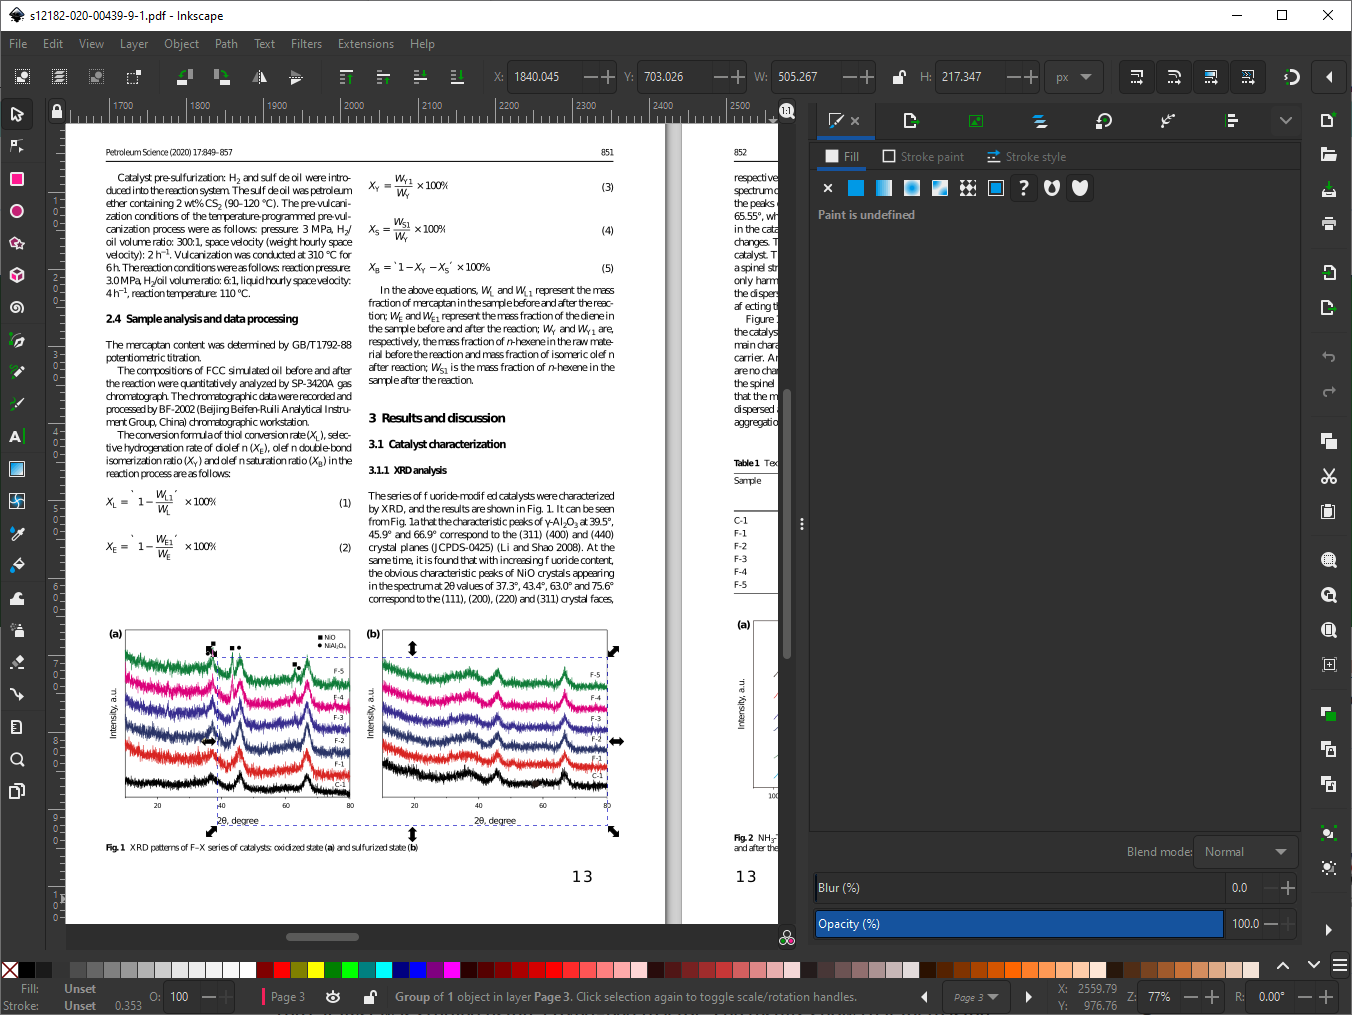
\includegraphics[width=\textwidth]{img/vector/in_inkscape.PNG}
    \caption*{Our PDF opened in Inkscape with the traces in Figure 1B selected.}
\end{figure}

\pagebreak
Next, repeatedly use \textbf{Right click > Ungroup (Shift + Ctrl + G)} on the selected objects until individual objects (in this case, individual line traces) can be selected.

\begin{figure}[h!tbp]
    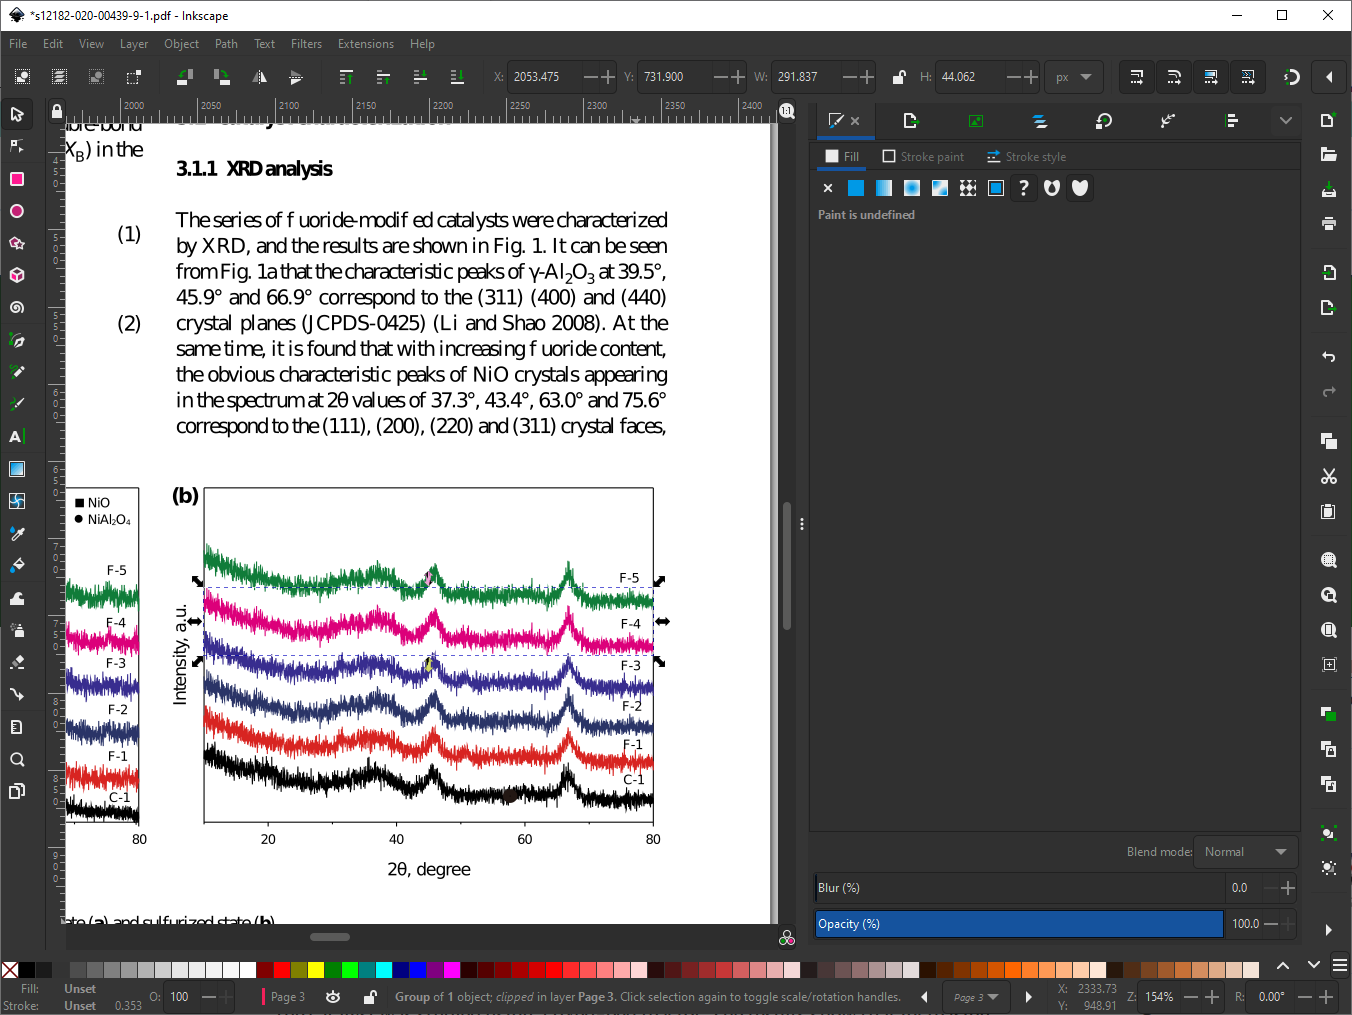
\includegraphics[width=\textwidth]{img/vector/in_inkscape_individual_traces.PNG}
    \caption*{After repeatedly ungrouping objects, we can now select individual line traces.}
\end{figure}

\pagebreak
When viewing line traces, it is helpful, but not necessary, to thin out the traces to enable comparison. To do so, navigate to \textbf{Objects > Fill and Stroke (Shift + Ctrl + F)}, under which the \textbf{Stroke Style} menu allows you to set line thickness. Afterwards, moving the traces to be closer to one another reveals that the F-2 (navy), F-4 (pink) and F-5 (green) traces are identical and the F-3 (blue) and F-1 (red) traces are identical.

\begin{figure}[h!tbp]
    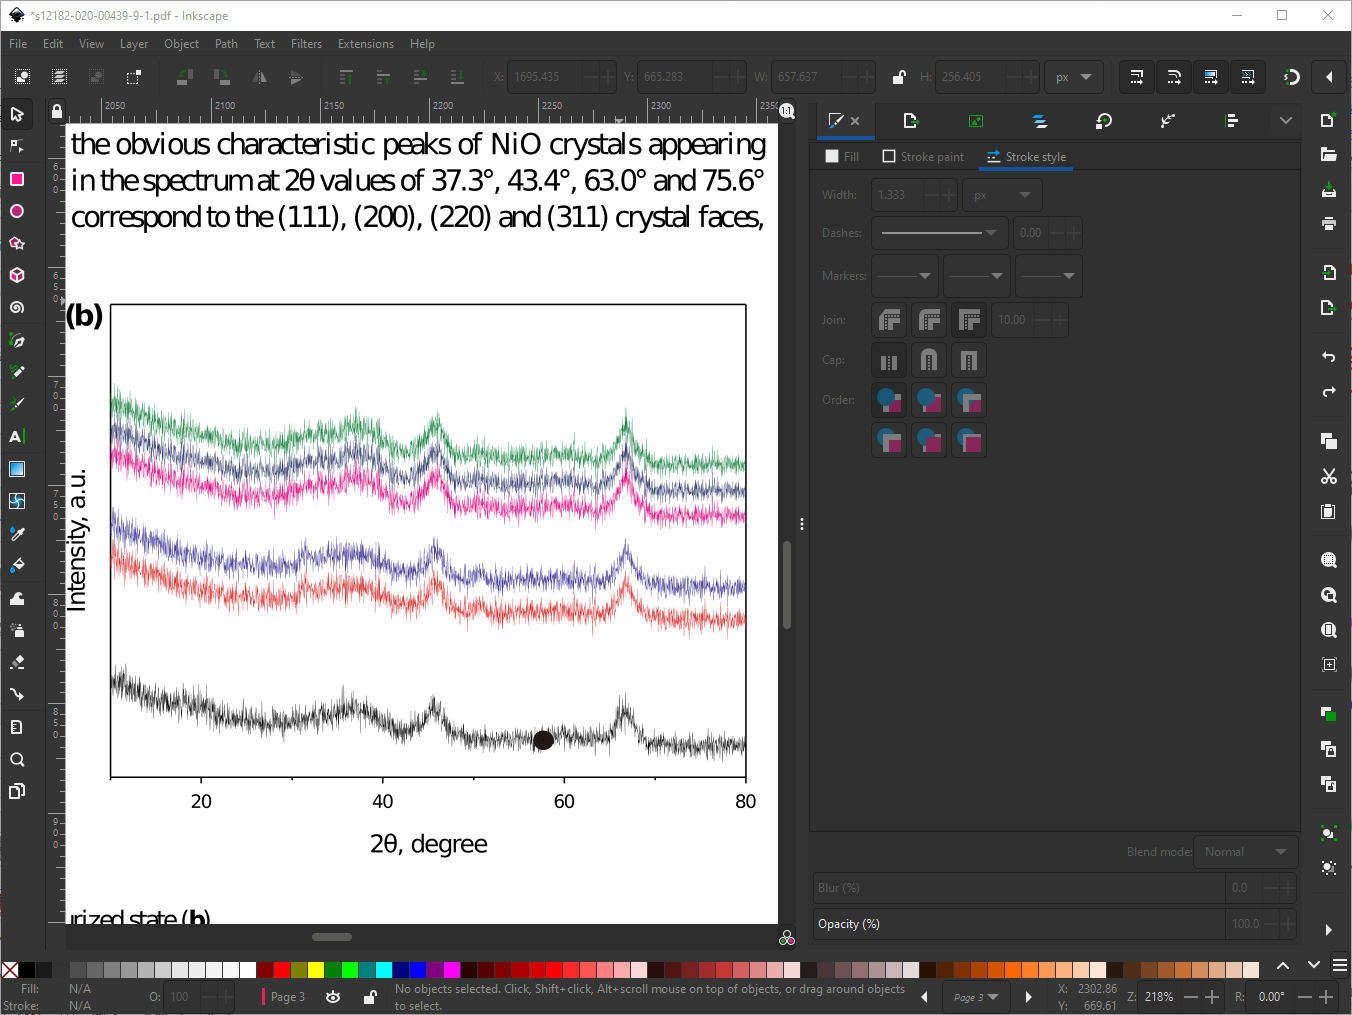
\includegraphics[width=\textwidth]{img/vector/in_inkscape_individual_traces_thinned.PNG}
    \caption*{Moving around and thinning out traces in Inkscape allows for easier comparison.}
\end{figure}

\pagebreak
We can also overlap the traces to make it crystal clear that these are the same data.

\begin{figure}[h!tbp]
    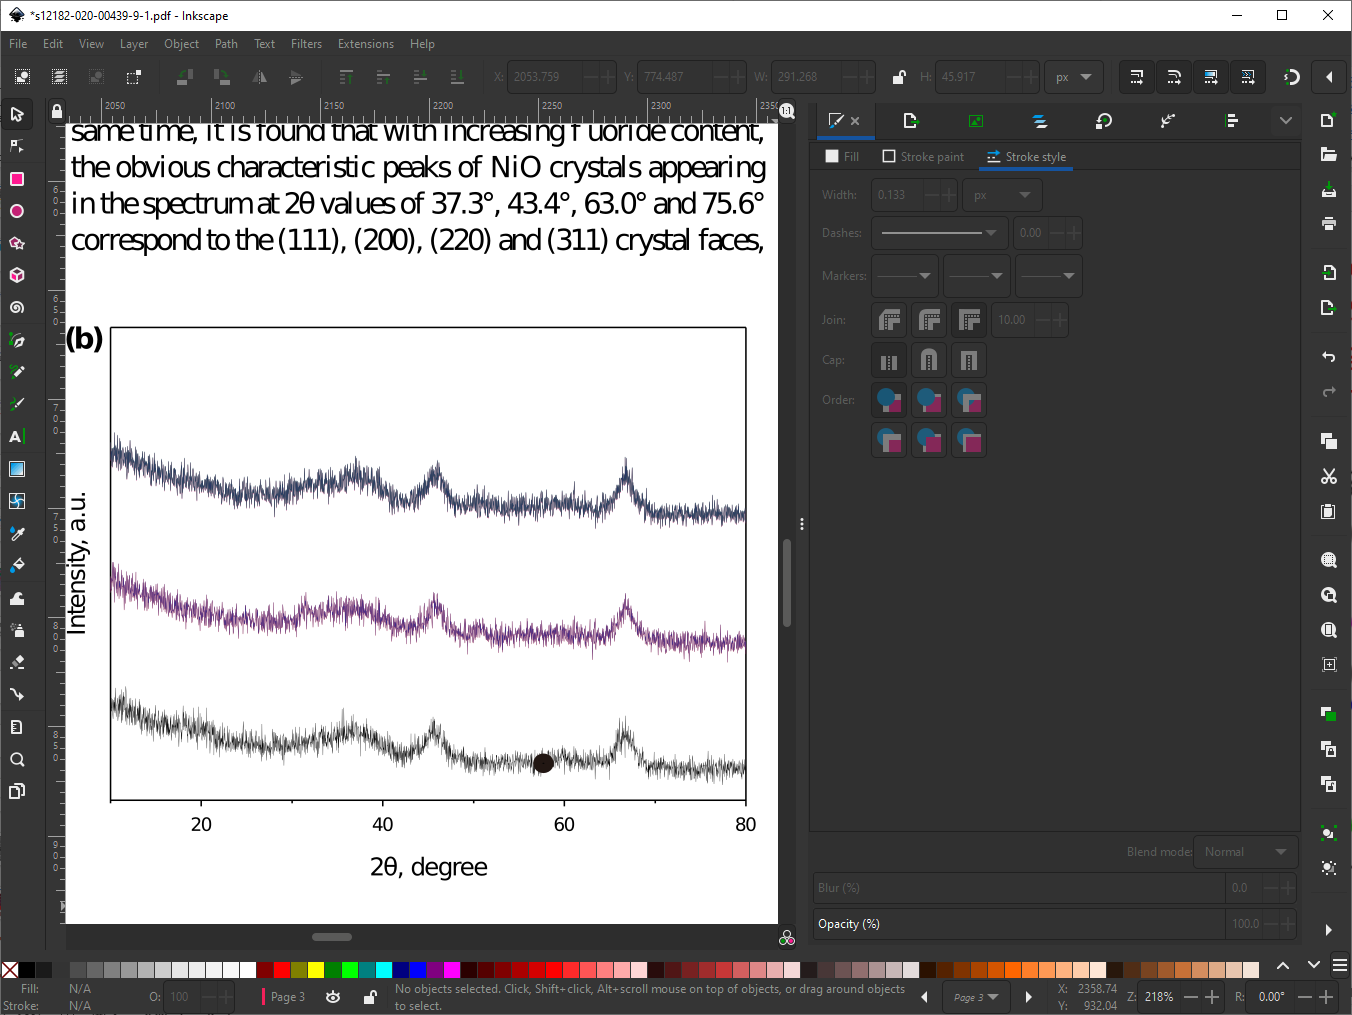
\includegraphics[width=\textwidth]{img/vector/in_inkscape_individual_traces_thinned_overlapping.PNG}
    \caption*{Now that traces are individual objects, we can easily overlap them to show that certain traces are identical.}
\end{figure}

\pagebreak
Objects can also be copy-pasted into a new document.

\begin{figure}[h!tbp]
    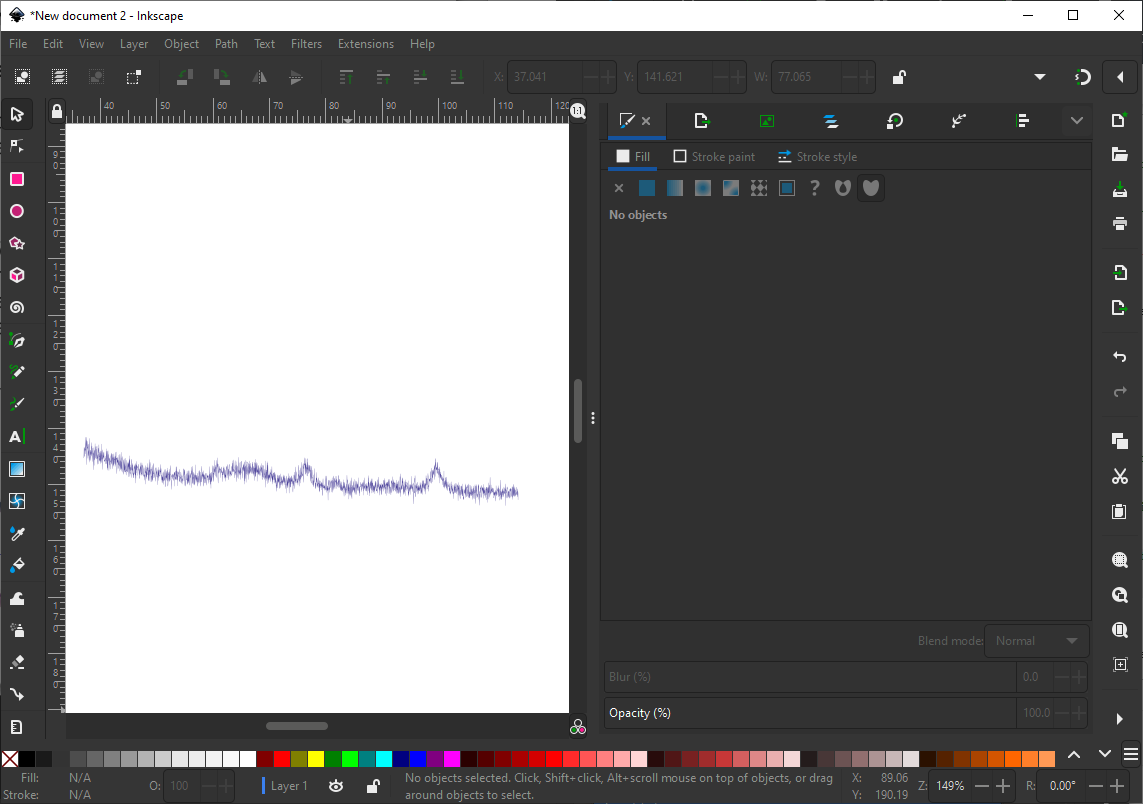
\includegraphics[width=\textwidth]{img/vector/inkscape_new_document.PNG}
    \caption*{ An individual trace copied into a new Inkscape document.}
\end{figure}

\end{document}
\documentclass[letterpaper, 12pt]{article}

\usepackage{geometry}
 \geometry{
 letterpaper,
 total={170mm,257mm},
 left=20mm,
 top=20mm,
 bottom=20mm
 }
\usepackage{graphicx} % Required for inserting images
\usepackage{authblk}
\usepackage{amssymb}
\usepackage{lipsum}
\usepackage{float}
\usepackage{times}
\usepackage{amsmath}
\usepackage[format=plain,
            labelfont={bf,it},
            textfont=it]{caption}
\captionsetup{justification=raggedright,singlelinecheck=false}
\usepackage{ragged2e}
\usepackage{longtable}
\usepackage{comment}
\usepackage{setspace}
\usepackage{fancyhdr}
\usepackage{titlesec}
\usepackage[hyperindex,breaklinks]{hyperref}
\hypersetup{
    colorlinks=true,
    linkcolor=blue,
    filecolor=magenta,      
    urlcolor=blue,
    pdftitle={Overleaf Example},
    pdfpagemode=FullScreen,
    }
% \usepackage{background} % add COSIG logo to page
\usepackage[T1]{fontenc}
\usepackage{helvet}
\renewcommand{\familydefault}{\sfdefault}
\pagenumbering{gobble}
\usepackage[skip=10pt plus1pt, indent=40pt]{parskip}

\begin{comment}
\backgroundsetup{
   scale=1,
   angle=0,
   opacity=1,
   color=black,
   contents={\begin{tikzpicture}[remember picture, overlay]
      \node at ([xshift=3cm,yshift=1cm] current page.south west)
            {
\includegraphics[width = 5cm]{img/home/241017_final_logo_mockup.png}}; %<- change the name of image
     \end{tikzpicture}}
 }
\end{comment}

\titlespacing*{\section}
{0pt}{1.5ex plus 1ex minus .2ex}{1.3ex plus .2ex}

\renewcommand\Authfont{\fontsize{12}{14.4}\selectfont}
\renewcommand\Affilfont{\fontsize{9}{10.8}\itshape}
 
\begin{document}
\flushleft

\includegraphics[width=0.5\textwidth]{img/home/241017_final_logo_mockup.png}

\section*{The vertical line test}
\addcontentsline{toc}{section}{The vertical line test}
\textit{Last updated: 7 February 2025}

For many types of data plotted on a x/y plane, it is expected that each x-axis value maps uniquely to a y-axis value. For instance, if you plotted your height over time, you would expect that each x-axis value (a point in time) corresponds to a single y-axis value (your height at that time). If not, this plot would imply that there were some points in your life where you were two different heights at the same time.

This property defines a \href{https://en.wikipedia.org/wiki/Graph_of_a_function}{mathematical function}, for which there is one unique output (y) for every unique input (x). The \href{https://en.wikipedia.org/wiki/Vertical_line_test}{vertical line test} is a simple method for gauging if a trace/curve is a function or not: given a trace/curve on an x/y plane, can you draw a vertical line that intersects the trace/curve multiple times? If there is at least one such vertical line, the trace/curve is not a mathematical function and may not make sense for the type of data it is describing.

\begin{figure}[h!tbp]
    \centering
    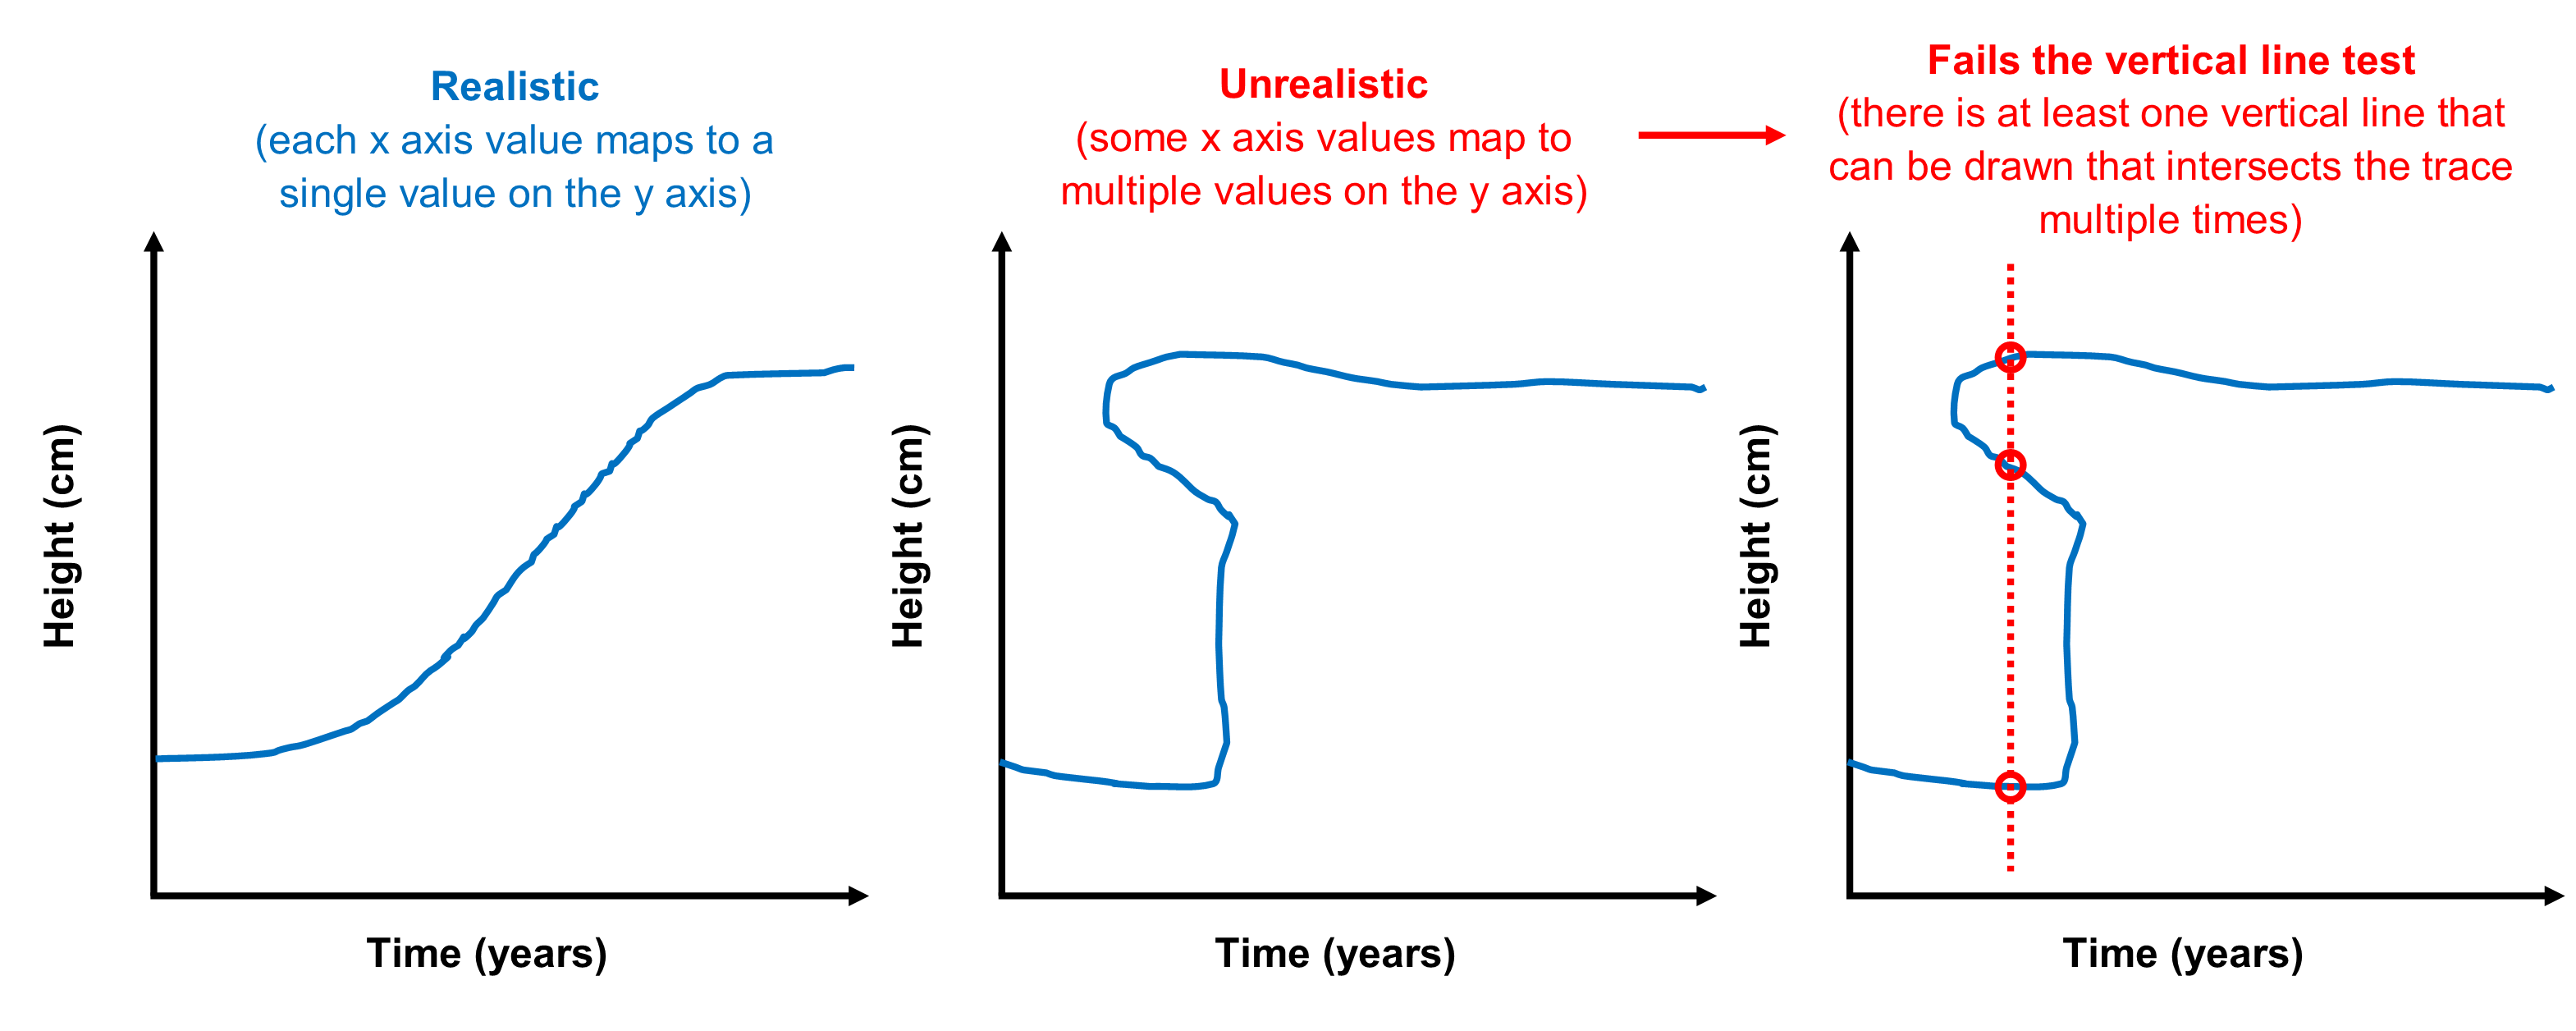
\includegraphics[width=\textwidth]{img/vertical_line/vertical_line_test_mockup.png}
    \caption*{If you plotted your height over time, you would expect each point in time (i.e., each point on the x axis) to correspond to a single height (i.e., a single point on the y axis). The graph on the left matches this expectation and is realistic for this kind of data. The graph in the middle does not match this expectation; there are some points in time that correspond to multiple heights. The graph on the right shows this trace failing the the vertical line test. This is just one of many vertical lines that could be drawn that show that this trace is not a function and thus does not realistically describe data representing height over time.}
\end{figure}

\pagebreak

\subsection*{Data types that should always pass the vertical line test}

Some data types, when plotted, will invariably be functions and thus should always pass the vertical line test. For instance, taking the absorption spectrum of a material should yield one value for absorption for every wavelength. Data types that are always expected to pass the vertical line test include, but are not limited to:

\begin{itemize}
    \setlength\itemsep{-0.5em}
    \item any \href{https://en.wikipedia.org/wiki/Absorption_spectroscopy}{light absorption spectrum}, including ultraviolet-visible (UV-VIS) absorption spectra, infrared (IR) absorption spectra, microwave absorption spectra, X-ray absorption spectra (XAS), etc. (\textit{Note that essentially anything that gets called a ``spectrum" should pass the vertical line test.})
    \item \href{https://en.wikipedia.org/wiki/Nuclear_magnetic_resonance_spectroscopy}{nuclear magnetic resonance (NMR)} spectra
    \item \href{https://en.wikipedia.org/wiki/Electron_paramagnetic_resonance}{electron spin resonance (ESR)/electron paramagnetic resonance (ESR)} spectra
    \item \href{https://en.wikipedia.org/wiki/Fourier-transform_infrared_spectroscopy}{Fourier-transform infrared (FTIR)} spectra
    \item \href{https://en.wikipedia.org/wiki/Raman_spectroscopy}{Raman} spectra
    \item \href{https://en.wikipedia.org/wiki/X-ray_diffraction}{X-ray diffraction (XRD)} patterns/diffractograms
    \item \href{https://en.wikipedia.org/wiki/Energy-dispersive_X-ray_spectroscopy}{energy-dispersive X-ray (EDX/EDS/EDAX)} spectra
    \item \href{https://en.wikipedia.org/wiki/X-ray_photoelectron_spectroscopy}{X-ray photoelectron} spectra (XPS)
    \item \href{https://en.wikipedia.org/wiki/Photoluminescence}{photoluminescence (PL)} spectra
    \item \href{https://en.wikipedia.org/wiki/Mass_spectrometry}{Mass spectra (MS/mass spec)}
    \item \href{https://en.wikipedia.org/wiki/Differential_thermal_analysis}{differential thermal analysis (DTA)} curves
    \item \href{https://en.wikipedia.org/wiki/Differential_scanning_calorimetry}{differential scanning calorimetry (DSC)} curves
    \item \href{https://en.wikipedia.org/wiki/Thermogravimetric_analysis}{thermogravimetric analysis (TGA)}curves
    \item \href{https://en.wikipedia.org/wiki/Transient_photocurrent}{photocurrent response/transient photocurrent (TPC)} curves
    \item \href{https://en.wikipedia.org/wiki/Electroencephalography}{electroencephalograms (EEG)}
    \item \href{https://en.wikipedia.org/wiki/Patch_clamp}{patch-clamp} recordings
\end{itemize}

\subsection*{Data types that may not pass the vertical line test}

For some data types, it is entirely expected that some x axis values will map to multiple y axis values. Data types that may or may not pass the vertical line test include, but are not limited to:

\begin{itemize}
    \setlength\itemsep{-0.5em}
    \item \href{https://en.wikipedia.org/wiki/Cyclic_voltammetry}{cyclic voltammetry (CV)} curves
    \item traces of an object moving in two dimensions, such as a mouse solving a \href{https://en.wikipedia.org/wiki/Morris_water_navigation_task}{Morris water navigation task}
    \item \href{https://en.wikipedia.org/wiki/Pressure%E2%80%93volume_diagram}{Pressure-volume (PV) diagrams}
    \item diagrams of \href{https://en.wikipedia.org/wiki/Graph_theory}{mathematical graphs/networks}
\end{itemize}

\pagebreak

\subsection*{Example 1: Passes the vertical line test}

\href{https://doi.org/10.1021/acsami.4c03997}{Thomas et al. (2024)} report using X-ray diffraction (XRD), Fourier-transform infrared spectroscopy (FTIR) and thermogravimetric analysis (TGA), among other techniques, to characterize kaolinite and kaolinite nanoplatelets. Each of these techniques yield data with one value on the y axis for each value on the x axis. All the plots corresponding to these techniques provided by Thomas et al. pass the vertical line test, as expected.

\begin{figure}[h!tbp]
    \centering
    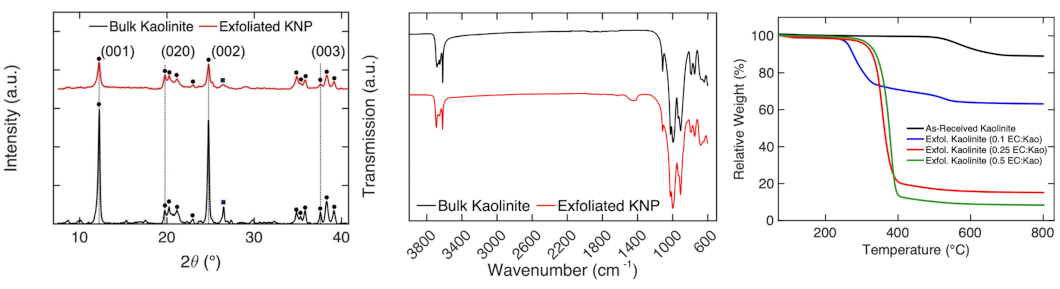
\includegraphics[width=\textwidth]{img/vertical_line/thomas_et_al_mockup.png}
    \caption*{Plots from \href{https://doi.org/10.1021/acsami.4c03997}{Thomas et al. (2024)} that pass the vertical line test (adapted from Figures 2B, S8 and S2).}
\end{figure}

\subsection*{Example 2: Does not pass the vertical line test}

\href{https://doi.org/10.1016/j.ceramint.2014.07.091}{Mandizadeh et al. (2014)} report using FTIR to characterize barium hexaferrite nanostructures. However, the FTIR spectrum they show backtracks on itself several times, failing the vertical line test.

\begin{figure}[h!tbp]
    \centering
    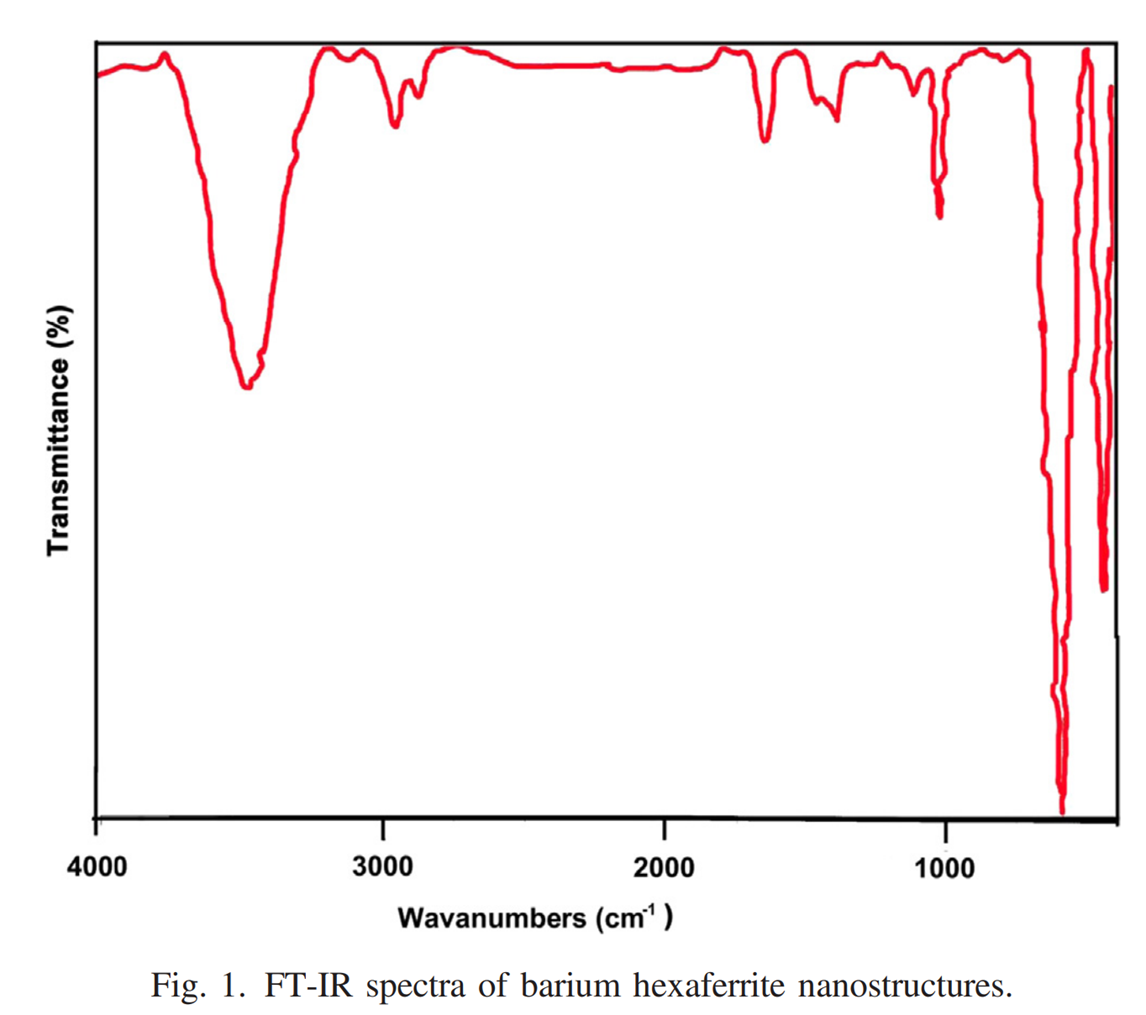
\includegraphics[width=0.6\textwidth]{img/vertical_line/mandizaeh_ftir.png}
    \caption*{An FTIR spectrum from Figure 1 of \href{https://doi.org/10.1016/j.ceramint.2014.07.091}{Mandizadeh et al. (2014)} that fails the vertical line test.}
\end{figure}

\pagebreak

\subsection*{Example 3: Does not pass the vertical line test}

\href{https://doi.org/10.1007/s10854-024-13064-8}{Suguna et al. (2024)} report using FTIR to characterize nanocomposite photocatalysts. However, the FTIR spectra they show appear to be hand-drawn and some fail the vertical line test.

\begin{figure}[h!tbp]
    \centering
    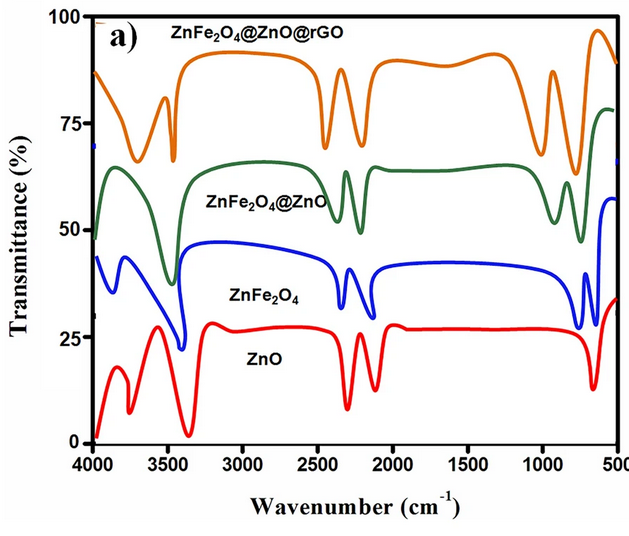
\includegraphics[width=\textwidth]{img/vertical_line/suguna_ftir.png}
    \caption*{FTIR spectra from Figure 3A \href{https://doi.org/10.1007/s10854-024-13064-8}{Suguna et al. (2024)}. The ZnFe$_2$O$_4$ spectrum (in blue) fails the vertical line test.}
\end{figure}

\pagebreak

\subsection*{Example 4: Vertical line test does not apply}

\href{https://doi.org/10.1371/journal.pcbi.1004110}{Lepora and Pezzulo (2015)} describe tracking mice in 2D space. They include several mouse trajectories in figures which follow the path of a mouse with a line. These trajectories are not expected to be functions and thus the vertical line test does not apply.

\begin{figure}[h!tbp]
    \centering
    \includegraphics[width=\textwidth]{img/vertical_line/pcbi.1004110.g002.png}
    \caption*{Mouse trajectory traces in 2D space, for which the vertical line test does not apply. Adapted from Figure 2 of \href{https://doi.org/10.1371/journal.pcbi.1004110}{Lepora and Pezzulo (2015)}.}
\end{figure}


\end{document}
\documentclass[letterpaper, 12pt]{article}

\usepackage{geometry}
 \geometry{
 letterpaper,
 total={170mm,257mm},
 left=20mm,
 top=20mm,
 bottom=20mm
 }
\usepackage{graphicx} % Required for inserting images
\usepackage{authblk}
\usepackage{amssymb}
\usepackage{lipsum}
\usepackage{float}
\usepackage{times}
\usepackage{amsmath}
\usepackage[format=plain,
            labelfont={bf,it},
            textfont=it]{caption}
\captionsetup{justification=raggedright,singlelinecheck=false}
\usepackage{ragged2e}
\usepackage{longtable}
\usepackage{comment}
\usepackage{setspace}
\usepackage{fancyhdr}
\usepackage{titlesec}
\usepackage[hyperindex,breaklinks]{hyperref}
\hypersetup{
    colorlinks=true,
    linkcolor=blue,
    filecolor=magenta,      
    urlcolor=blue
    }
% \usepackage{background} % add COSIG logo to page
\usepackage[T1]{fontenc}
\usepackage{helvet}
\renewcommand{\familydefault}{\sfdefault}
\pagenumbering{gobble}
\usepackage[skip=10pt plus1pt, indent=40pt]{parskip}

\titlespacing*{\section}
{0pt}{1.5ex plus 1ex minus .2ex}{1.3ex plus .2ex}

\renewcommand\Authfont{\fontsize{12}{14.4}\selectfont}
\renewcommand\Affilfont{\fontsize{9}{10.8}\itshape}
 
\begin{document}
\flushleft
\includegraphics[width=0.5\textwidth]{img/home/241017_final_logo_mockup.png}

\section*{Suspicious venues}
\addcontentsline{toc}{section}{Suspicious venues}
\textit{Last updated: 3 June 2025}

Problematic articles repeatedly showing up in the same publication venue (e.g., journal, conference, book, etc.) can raise warning signs about the venue itself. A well-structured and thorough peer review system is unlikely to result in frequent publication of glaringly problematic articles.

When venues are implicated or exhibit red flags on their own, it can indicate that the articles they published deserve additional scrutiny.
This does not always indicate the publisher itself is malicious, as many publishers do not closely scrutinize the articles they publish.
Thus, legitimate world-renowned venues can share a publisher with shady venues that publish obvious nonsense (see problematic articles published in \href{https://solalpirelli.github.io/2023/01/25/troubling-acm-venues.html}{Association for Computing Machinery conferences} and \href{https://deevybee.blogspot.com/2025/02/ieee-has-pseudoscience-problem.html}{Institute of Electrical and Electronics Engineers conferences}).

This guide covers common warning signs that a publication venue deserves additional scrutiny. Many additional warning signs are described by \href{https://doi.org/10.1177/0192623320920209}{Elmore et al. (2020)}.

\subsection*{Missing or outdated information}

The organizers of unethical venues are not interested in spending any more time than is necessary.
This often results in venue websites that are not up to date or outright broken outside of the main page.

Would a reasonable person easily find the information they need to gauge their interest,
write a manuscript with the right specifications, and submit that manuscript?
For a conference, would this reasonable person also easily know when and where the conference is held and how to get there?

Missing information, copy-pasted text from previous years that contains outdated dates and times,
and ``404 Not Found'' pages are all red flags.
Sometimes the information looks real, but a quick check will reveal it is not,
such as international conferences supposedly taking place in buildings that are
obviously not suitable for a large number of attendees nor for presentations or \href{https://doi.org/10.1038/d41586-024-02358-w}{multiple conferences taking place in the same location on the same day} (except for conferences that officially advertise their ``co-location'' with another conference).

\subsection*{Overemphasis on metrics}

Scientists and institutions around the globe are often evaluated using quantitative heuristics such as number of articles published in indexed journals and number of citations to those articles (see \href{https://osf.io/5vknq}{COSIG's citations guide}). Unethical and predatory venues often emphasize common metrics well beyond how a reasonable venue would.

Unethical venues may include in their description the fact they are Scopus-indexed,
the fact that proceedings will be published with a specific well-known publisher (without providing any additional details)
and other information that should be obvious and unstated for any reputable venue.
If a venue tries too hard to convince you that it is legitimate, it likely is not.

\subsection*{Malicious compliance with integrity standards}

To be attractive in terms of metrics such as indexing in a particular database,
unethical venues often abuse the trust of a reputable publisher.
Reputable publishers try to maintain their reputation with basic integrity standards, such as the absence of plagiarism (see \href{https://osf.io/ntcb4}{COSIG's plagiarism guide}).

Unethical venues work around this by turning subjective checks into objective ones
and giving enough information to authors to avoid detection.
For instance, submissions to a venue will often be assessed by a human with the help of a tool such as
\href{https://www.ithenticate.com/}{iThenticate}.
To work around this, a malicious editor-in-chief can publicly state which tool will be used
and which exact threshold will be used on the tool output to make a binary assessment of plagiarism.
Thus, authors wishing to plagiarize only need to spend as little time as necessary hiding their plagiarism
until the tool's output is below the threshold.
Any ``plagiarism score'' threshold indicates a problematic venue.

\subsection*{Unrealistic review time}

Sending manuscripts for peer review, receiving the reviews, and coming to a decision takes time.
Turnaround times can be shorter for venues that have specific deadlines, such as conferences,
since finding the reviewers is already done and these reviewers know to block time in their calendar.
However, peer review time is still normally measured in months. There is also no guarantee that a submission that goes out to peer review will actually be accepted.

Guaranteed time to acceptance should be regarded with extreme suspicion. Any venue that advertises an extremely short review period (unless submissions are very short, e.g., only abstracts) is likely predatory or unethical.

Journals will often list the time between submission and acceptance, allowing for estimation of times to publication. Suspicious venues will often routinely accept manuscripts from particular authors in a matter of days, not nearly long enough for legitimate peer review to occur.
which often state when they were submitted and accepted.
This can reveal unethical patterns where manuscripts from some authors are supposedly reviewed in days.
(\href{https://deevybee.blogspot.com/2015/02/editors-behaving-badly.html}{example})

Note that not all journals provide accurate submission information. Sometimes, the listed ``submission'' date is really a resubmission after revisions were requested by reviewers.

\subsection*{Unethical editors}

Unethical venues can often be spotted by suspicious behavior by their editors.

While it is normal for well-known scientists to chair well-known venues while also publishing in them,
some editors do not stop at the low number of articles one would expect from a reputable scientist,
and instead \href{https://deevybee.blogspot.com/2020/08/pepiops-prolific-editors-who-publish-in.html}{publish dozens of articles in their own venue}, abusing their position of power.

Venues that publish articles wherein \href{https://pubpeer.com/publications/57BB3F8859A0F5BE6FBC4DB70F2E8E}{an outsized portion of an article's citations are to the venue's editor(s)} should be regarded with extreme suspicion. Citing multiple articles from the editor of the venue
can be acceptable if that person has published foundational work,
but many articles in a venue all citing the exact same set of articles from the editors is unexpected.

\subsection*{Fake committees}

Unethical venues will often project legitimacy by listing legitimate scientists' names as conference organizers, editors or peer reviewers without their knowledge or consent. These venues might fabricate affiliations or contact information alongside the names of real scientists or might use real scientists' pictures to represent fictitious identities. 

If you suspect reviewer names are being used without their knowledge, find the contact information for the reviewers
using a source unrelated to the venue under suspicion and contact them. Most institutions provide some form of public profile for researchers,
even if it is merely a directory entry with just a name.
If you suspect a reviewer identity or affiliation has been fabricated, find a contact at the provided affiliation and ask.

\subsection*{Hijacked journals}

Often illegitimate publishers will `hijack' existing legitimate journals by creating a website that mimics that of the existing journal, using the existing journal's name and/or \href{https://portal.issn.org/}{International Standard Serial Number}, or registering the existing journal's domain after it has expired. Having hijacked the existing journal's brand, the illegitimate publisher can now publish whatever content it pleases while enjoying the benefits of the journal's existing reputation (including membership in curated literature databases, see `Indexing and de-indexing' below).

The \href{https://retractionwatch.com/the-retraction-watch-hijacked-journal-checker/}{Retraction Watch Hijacked Journal Checker} is an updating directory of journals that have been hijacked.

\pagebreak

\begin{figure}[h!tbp]
    \centering
    \includegraphics[width=\textwidth]{img/venues/Preslia original.png}
    \caption*{The homepage of the legitimate journal Preslia, a publication of the Czech Botanical Society, at \href{https://www.preslia.cz}{www.preslia.cz}.}
\end{figure}

\begin{figure}[h!tbp]
    \centering
    \includegraphics[width=\textwidth]{img/venues/Preslia hijacked-min.png}
    \caption*{The homepage of a hijacked version of Preslia at \href{https://presliajournal.com/}{www.presliajournal.com}. Note that the hijacked journal appropriates Preslia's ISSN and claims to accept articles on any topic, despite the actual Preslia being solely a botany journal.}
\end{figure}

\subsection*{Raising suspicions about a venue on PubPeer}

To report concerning trends in a venue's articles, you can write a lengthy PubPeer comment on one article
and short comments on the others linking to the main comment (see \href{https://osf.io/sghaq}{COSIG's guide on PubPeer commenting}).
Alternatively, if there is a DOI representing the totality of articles in a venue (e.g., front matter for a conference or an article listing journal editorial board members), considering writing a \href{https://pubpeer.com/search?q=\%22proceedings-level+report\%22}{``proceedings-level report''} or \href{https://pubpeer.com/search?q=\%22journal-level+report\%22}{``journal-level report''}.

\subsection*{Indexing and de-indexing}

Publication venues are `indexed' by literature aggregators like \href{https://www.webofscience.com/wos/}{Web of Science}, \href{https://www.scopus.com}{Scopus} and \href{https://www.nlm.nih.gov/medline/medline_home.html}{MEDLINE} and in databases like the \href{https://doaj.org/}{Directory of Open Access Journals (DOAJ)}. Being indexed by one of these services is perceived as a marker of quality for publication venues. Many predatory venues advertise their indexing status because they know that many academics are required to publish articles only in indexed venues. These services will sometimes withdraw the indexing status of , or `de-index', particular venues because of a pattern of publication integrity issues or other ethical violations (for example, see the \href{https://docs.google.com/spreadsheets/d/1Kv3MbgFSgtSDnEGkA2JacrSjunRu0umHeZCtcMeqO5E/edit?gid=2104690845\#gid=2104690845}{list of journals withdrawn from DOAJ}, many of which have been removed for ``not adhering to Best Practice''). If you have suspicions about a venue and it is indexed by one of these services, consider reporting your concerns to the service.

\subsection*{Additional resources}

\begin{itemize}
    \setlength\itemsep{-0.5em}
    \item \href{https://doi.org/10.1177/0192623320920209}{``Predatory Journals: What They Are and How to Avoid Them'' (2020)}
    \item \href{https://retractionwatch.com/2024/10/01/hidden-hydras-uncovering-the-massive-footprint-of-one-paper-mills-operations/}{``Hidden hydras: uncovering the massive footprint of one paper mill’s operations'' (2024)}
    \item \href{https://deevybee.blogspot.com/2015/02/editors-behaving-badly.html}{``Editors behaving badly?'' (2015)}
    \item \href{https://deevybee.blogspot.com/2024/09/using-pubpeer-to-screen-editors.html}{``Using PubPeer to screen editors'' (2024)}
    \item \href{https://deevybee.blogspot.com/2020/08/pepiops-prolific-editors-who-publish-in.html}{``PEPIOPs – prolific editors who publish in their own publications'' (2020)}
    \item \href{https://www.science.org/content/article/it-felt-very-icky-scientist-s-name-was-used-write-fake-peer-reviews}{```It felt very icky': This scientist's name was used to write fake peer reviews'' (2024)}
    \item \href{https://doi.org/10.47989/irpaper912}{``Membership of the editorial boards of journals published by the predatory publisher OMICS: willing and unwilling participation'' (2021)}
    \item \href{https://doi.org/10.1038/543481a}{``Predatory journals recruit fake editor'' (2017)}
    \item \href{https://doi.org/10.18421/GP19.02-06}{``The full story of 90 hijacked journals from August 2011 to June 2015'' (2015)}
    \item \href{https://retractionwatch.com/2020/07/07/the-case-of-the-stolen-journal/}{``The case of the stolen journal'' (2020)}
    \item \href{https://doi.org/10.1007/s11192-021-04056-0}{``Detecting a network of hijacked journals by its archive'' (2021)}
    \item \href{https://doi.org/10.1002/asi.24855}{``Challenges posed by hijacked journals in Scopus'' (2023)}
    \item \href{https://doi.org/10.1080/08989621.2024.2387210}{``Prevalence of plagiarism in hijacked journals: A text similarity analysis'' (2024)}
    \item \href{https://doi.org/10.1126/science.zcgp0a2}{``Leading scholarly database listed hundreds of papers from ‘hijacked’ journals'' (2023)}
    \item \href{https://retractionwatch.com/the-retraction-watch-hijacked-journal-checker/}{The Retraction Watch Hijacked Journal Checker}
\end{itemize}

\end{document}

% Biology and medicine
\documentclass[letterpaper, 12pt]{article}
\usepackage{geometry}
\geometry{
    letterpaper,
    left=20mm,
    top=20mm,
    bottom=20mm
}
\usepackage{tocloft}
\usepackage{graphicx}
\usepackage{authblk}
\usepackage{amssymb}
\usepackage{lipsum}
\usepackage{float}
\usepackage{times}
\usepackage{amsmath}
\usepackage[format=plain,
            labelfont={bf,it},
            textfont=it]{caption}
\captionsetup{justification=raggedright,singlelinecheck=false}
\usepackage{ragged2e}
\usepackage{longtable}
\usepackage{comment}
\usepackage{setspace}
\usepackage{fancyhdr}
\usepackage{titlesec}
\usepackage[hyperindex,breaklinks]{hyperref}
\hypersetup{
    colorlinks=true,
    linkcolor=blue,
    filecolor=magenta,      
    urlcolor=blue
}
\usepackage[T1]{fontenc}
\usepackage{helvet}
\renewcommand{\familydefault}{\sfdefault}
\pagenumbering{gobble}
\usepackage[skip=10pt plus1pt, indent=40pt]{parskip}
\usepackage{orcidlink}
\usepackage{standalone}

\titlespacing*{\section}
{0pt}{1.5ex plus 1ex minus .2ex}{1.3ex plus .2ex}

\renewcommand\Authfont{\fontsize{12}{14.4}\selectfont}
\renewcommand\Affilfont{\fontsize{9}{10.8}\itshape}

\newcommand{\cosigpart}[1]{
  \addcontentsline{toc}{part}{#1}
}
\newcommand{\cosigsection}[1]{
  \section*{#1}
  \phantomsection % avoid warnings from hyperref about the anchor of a bookmark and its parent's
  \addcontentsline{toc}{section}{#1}
}
\begin{document}
\flushleft\includegraphics[width=0.5\textwidth]{img/home/241017_final_logo_mockup.png}

\cosigpart{Biology and medicine}
\cosigsection{Antibody validation}
\textit{Last updated: 14 May 2025}

Antibodies are a very common and exceptionally useful reagent in biomedical studies. Antibodies are designed to bind to a specific kind of protein, allowing scientists to isolate that protein on a gel, tag that protein with a fluorescent probe, etc.

Antibodies are typically purchased from large laboratory supply vendors. Ideally, antibodies should be selective (i.e., they bind strongly to the protein of interest) and specific (i.e., they only bind strongly to one protein of interest). However, commercially-available antibodies can be plagued by a variety of issues:

\begin{itemize}
    \setlength\itemsep{-0.5em}
    \item \textbf{Lack of specificity:} An antibody could bind non-specifically to a number of other proteins aside from its target protein.
    \item \textbf{Lack of selectivity:} An antibody could fail to bind strongly to its target protein.
    \item \textbf{Variability in quality:} Different batches of antibody manufactured by the same provider may not perform as well as others.
    \item \textbf{Specificity to conformation:} It is possible that an antibody binds a protein only in its folded state or its unfolded state. Depending on the application, researchers may prefer an antibody that is selective and specific to one of these conformations. Even if an antibody does not bind selectively or specifically to a protein in its folded state, it may bind to the protein in its unfolded state and may still be suitable for use in application where the protein is expected to be unfolded (or vice versa).
    \item \textbf{Specificity to isoform:} The same protein can exist as a variety of \href{https://en.wikipedia.org/wiki/Protein_isoform}{isoforms}. An antibody may more effectively target one of a protein's isoforms over another.
\end{itemize}

Several initiatives have been launched to improve the quality of antibodies and the reproducibility of studies using them:

\begin{itemize}
    \setlength\itemsep{-0.5em}
    \item \textbf{\href{https://www.antibodypedia.com/}{Antibodypedia}} is an online platform that documents the level of support thousands of commercially-available antibodies have for various applications.
    \item \textbf{\href{https://www.antibodyregistry.org}{The Antibody Registry}} is an online platform that allows users to catalog the antibodies that they use in their research with rich metadata and provenance tracking (useful if an antibody is no longer sold by a vendor).
    \item \textbf{\href{https://www.citeab.com}{CiteAb}} is a service that tracks the uses of specific reagents, including antibodies, in the biomedical literature.
    \item \textbf{\href{https://www.proteinatlas.org/about/antibody+validation}{The Human Protein Atlas}} provides antibody validation data for antibodies that the project produces internally and collects validation data from suppliers for antibodies that are commercially available. 
    \item \textbf{\href{https://pabmabs.com/}{pAbmAbs}} allows users to rate antibodies out of five stars for their overall performance and for different applications.
    \item \textbf{\href{https://www.labome.com/index.html}{The Validated Antibody Database}} curates articles using and validating antibodies and collects reviews of antibodies used for a number of popular protein targets.
    \item \textbf{\href{https://ycharos.com/}{YCharos (Antibody Characterization through Open Science)}} is a non-profit that performs systematic validation of commercially-available antibodies, making their results openly available online.
\end{itemize}

This guide covers several common applications for antibodies and how they are validated for these applications according to the \href{https://doi.org/10.1038/s41596-024-01095-8}{protocol developed by YCharOS}. 

YCharOS tests antibodies in wild-type (WT) cell lines expressing the protein of interest and in knockout (KO) cell lines in which the protein of interest is `knocked out' by removing the gene encoding that protein from the cell line's genome with \href{https://en.wikipedia.org/wiki/CRISPR_gene_editing}{CRISPR-Cas9} technology.

\pagebreak

\subsection*{Western blotting/immunoblotting}

A Western blot usually involves separating proteins from cells (either from cell media for secreted proteins or from cell lysate for proteins expected to be internal to cells), separating proteins in this media/extract by running them on an \href{https://en.wikipedia.org/wiki/SDS-PAGE.}{SDS-PAGE} gel. This denatures the protein (although other varieties of gel, such as \href{https://www.med.unc.edu/pharm/sondeklab/wp-content/uploads/sites/868/2018/10/Native-gel-analysis.pdf}{native PAGE}, preserve the conformation of the protein in its native, folded state). After this, the contents of the gel are transferred to a membrane. A primary antibody that binds to the protein of interest is added to the membrane, followed by a secondary antibody that binds to the primary antibody and makes it detectable.

YCharos \href{https://f1000research.com/gateways/ycharos/faqs}{states}:

\begin{quote}
    \textit{A successful antibody immunodetects the target protein, and the signal observed in the wild-type (WT) lysate is lost in the knockout (KO) lysates. Ideally, the antibody also does not recognize any other protein under the conditions tested.}
\end{quote}

\begin{figure}[h!tbp]
    \centering
    \includegraphics[width=0.9\textwidth]{img/antibody_val/ycharos_wb.jpg}
    \caption*{Schematic illustrating expected outcomes for a successful antibody (left), for a successful antibody that non-specifically binds the protein of interest (center) and a non-successful antibody (right). Adapted from Table 3 of \href{https://doi.org/10.12688/f1000research.155929.2}{Ru\'iz Mole\'on et al. (2025).}}
\end{figure}

\pagebreak

\subsection*{Immunoprecipitation}

In immunoprecipitation, an antibody targeting a specific protein is conjugated to beads. These beads are mixed into a starting material (SM, cell media or cell lysate), wherein the protein of interest is immunocaptured by the antibody-conjugated beads. These beads are spun out of the mixture, leaving an unbound fraction (UB) and an immunoprecipitate (IP). To quantify how much of the protein is in the SM, UB and IP, a Western blot is performed using all three fractions and an antibody targeting the protein of interest validated for Western blotting.

Antibodies that are successful for immunoprecipitation generally target the protein of interest in its native, folded state. YCharOS \href{https://f1000research.com/gateways/ycharos/faqs}{states}:

\begin{quote}
    \textit{Under the conditions used, a successful antibody immunocaptures the target protein to at least 10\% of the starting material, which leads to an observable depletion of the target protein from the starting material.}
\end{quote}

\begin{figure}[h!tbp]
    \centering
    \includegraphics[width=0.9\textwidth]{img/antibody_val/ycharos_ip.jpg}
    \caption*{Schematic illustrating expected outcomes for a successful antibody that heavily depletes the target protein from the SM (left), a successful antibody that less heavily depletes the target protein from the SM (center) and a non-successful antibody (right). Adapted from Table 3 of \href{https://doi.org/10.12688/f1000research.155929.2}{Ru\'iz Mole\'on et al. (2025)}.}
\end{figure}

\pagebreak

\subsection*{Immunofluorescence}

In immunofluorescence, cells are \href{https://en.wikipedia.org/wiki/Fixation_(histology)}{fixed}, \href{https://doi.org/10.1007/978-1-59745-324-0_9}{permeabilized} and stained with an antibody conjugated to a fluorophore. This antibody will bind to the protein of interest within the cell, localize itself to the region of the cell that the protein inhabits. To validate antibodies with immunofluorescence, YCharOS takes fluorescence images of WT and KO cells plated together as a `mosaic'.  The WT and KO cells are labeled with fluorophores of different wavelengths so that they can be differentiated from one another. For intracellular proteins (i.e., not secreted), fluorescence signal for the protein of interest should be pronounced in the WT cell line, negligible in the KO cell line and negligible in the background. 

Antibodies that are successful for immunofluorescence generally target the protein of interest in its native, folded state. YCharos \href{https://f1000research.com/gateways/ycharos/faqs}{states}:

\begin{quote}
    \textit{A successful antibody immunolocalizes the target protein by generating a signal in WT cells that is at least 1.5-fold over the signal in KO cells. Signal provided by such antibody can be easily distinguished from background noise.}
\end{quote}

\begin{figure}[h!tbp]
    \centering
    \includegraphics[width=0.9\textwidth]{img/antibody_val/ycharos_if.jpg}
    \caption*{Schematic illustrating expected outcomes for a successful antibody that localizes to the protein of interest in the WT but not KO (left) and an unsuccessful antibody that does not localize to the protein of interest (as made evident by the equivalent signal in the KO cell line, right).}
\end{figure}

\subsection*{Example 1: Bax Antibody (B-9)}

Bax Antibody (B-9) (sold by Santa Cruz Biotechnology under catalog number \href{https://www.scbt.com/p/bax-antibody-b-9}{sc-7480}) has been used in more than 1,000 articles to target \href{https://en.wikipedia.org/wiki/Apoptosis_regulator_BAX}{Bax}, a widely-studied regular of apoptosis, in rat, mouse and human cells. However, \href{https://doi.org/10.1038/s41419-024-07273-6}{Entrop et al. (2024)} report on validation studies using using WT and Bax-deficient cell lines (as well as cell lines through which Bax has been depleted with \href{https://en.wikipedia.org/wiki/Small_interfering_RNA}{siRNA}) through which they find that Bax Antibody (B-9) likely does not target Bax. Instead, the antibody likely targets another protein at a similar molecular weight. Bax is a widely-studied gene and there are hundreds of other Bax-targeting antibodies available from a number of providers.

\subsection*{Additional resources}

\begin{itemize}
    \setlength\itemsep{-0.5em}
    \item \href{https://doi.org/10.1038/s41596-024-01108-6}{``YCharOS protocol for antibody validation'' (2024)}
    \item \href{https://f1000research.com/ycharos}{YCharOS F1000 Research Gateway}
    \item \href{https://zenodo.org/communities/ycharos/records?q=&l=list&p=1&s=10&sort=newest}{YCharos Zenodo community}
    \item \href{https://doi.org/10.1038/d41586-024-03590-0}{``The antibodies don’t work! The race to rid labs of molecules that ruin experiments'' (2024)}
    \item \href{https://doi.org/10.1038/521274a}{``Reproducibility crisis: Blame it on the antibodies'' (2015)}
    \item \href{https://doi.org/10.1038/nmeth.3472}{``Assessment of a method to characterize antibody selectivity and specificity for use in immunoprecipitation'' (2015)}
    \item \href{https://doi.org/10.1038/s41419-024-07273-6}{``Why Bax detection in >1400 publications might be flawed'' (2024)}
    \item \href{https://doi.org/10.1007/s00210-009-0395-y}{``How reliable are G-protein-coupled receptor antibodies?'' (2009)}
\end{itemize}

\end{document}
\documentclass[letterpaper, 12pt]{article}

\usepackage{geometry}
 \geometry{
 letterpaper,
 total={170mm,257mm},
 left=20mm,
 top=20mm,
 bottom=20mm
 }
\usepackage{graphicx} % Required for inserting images
\usepackage{authblk}
\usepackage{amssymb}
\usepackage{lipsum}
\usepackage{float}
\usepackage{times}
\usepackage{amsmath}
\usepackage[format=plain,
            labelfont={bf,it},
            textfont=it]{caption}
\captionsetup{justification=raggedright,singlelinecheck=false}
\usepackage{ragged2e}
\usepackage{longtable}
\usepackage{comment}
\usepackage{setspace}
\usepackage{fancyhdr}
\usepackage{titlesec}
\usepackage[hyperindex,breaklinks]{hyperref}
\hypersetup{
    colorlinks=true,
    linkcolor=blue,
    filecolor=magenta,      
    urlcolor=blue,
    pdftitle={Overleaf Example},
    pdfpagemode=FullScreen,
    }
% \usepackage{background} % add COSIG logo to page
\usepackage[T1]{fontenc}
\usepackage{helvet}
\renewcommand{\familydefault}{\sfdefault}
\pagenumbering{gobble}
\usepackage[skip=10pt plus1pt, indent=40pt]{parskip}

\begin{comment}
\backgroundsetup{
   scale=1,
   angle=0,
   opacity=1,
   color=black,
   contents={\begin{tikzpicture}[remember picture, overlay]
      \node at ([xshift=3cm,yshift=1cm] current page.south west)
            {\includegraphics[width = 5cm]{img/home/241017_final_logo_mockup.png}}; %<- change the name of image
     \end{tikzpicture}}
 }
\end{comment}

\titlespacing*{\section}
{0pt}{1.5ex plus 1ex minus .2ex}{1.3ex plus .2ex}

\renewcommand\Authfont{\fontsize{12}{14.4}\selectfont}
\renewcommand\Affilfont{\fontsize{9}{10.8}\itshape}
 
\begin{document}
\flushleft
\includegraphics[width=0.5\textwidth]{img/home/241017_final_logo_mockup.png}

\section*{Misidentified and non-verifiable cell lines}
\textit{Last updated: 5 February 2025}
\subsection*{Cell lines}

A cell line is a population of cells that can be grown in a laboratory culture indefinitely. Cell lines are an essential tool for biomedical research because they allow biological experiments to be performed in vitro (i.e. outside of a living organism). For instance, researchers developing new cancer drugs will certainly test the effect of their drug candidates on many different cancer cell lines before ever considering testing the drug candidate on live animals, let alone human patients.

Because cell lines can grow indefinitely, one research laboratory or laboratory supplier can take a few cells from their cell line stock and give them to another laboratory for that laboratory to begin culturing their own stock. By far the most popular cell line is HeLa, and the many thousands of \href{https://www.cellosaurus.org/CVCL_0030}{HeLa cell stocks} used in biomedical research around the world can all be traced back to the original stock of "immortal" cervical cancer cells taken from \href{https://en.wikipedia.org/wiki/Henrietta_Lacks}{Henrietta Lacks in 1951}.

\subsection*{Misidentified/contaminated cell lines}

One complication of relying on cell lines for biomedical research is that stocks will often become cross-contaminated by other cell lines. For instance, HeLa is extremely aggressive as cancer cell lines go and HeLa cells will easily overtake other cell line stocks that are stored nearby. The popular gastric cancer cell line \href{https://www.cellosaurus.org/CVCL_3360}{BGC-823} is one such victim of HeLa’s aggression; there are no remaining uncontaminated stocks of BGC-823 and thus it is no longer considered an appropriate experimental model for gastric cancer.


\begin{figure}[h!tbp]
    \includegraphics[width=\textwidth]{img/cell_lines/Screenshot 2024-11-04 at 11-59-23 Cellosaurus cell line BGC-823 (CVCL_3360).png}
    \caption*{The Cellosaurus entry for \href{https://www.cellosaurus.org/CVCL_3360}{BGC-823} now warns about the cell line being contaminated by HeLa.}
\end{figure}

The International Cell Line Authentication Committee maintains \href{https://iclac.org/databases/cross-contaminations/}{a register of misidentified cell lines} that is currently 593 entries long. A good number of these cell lines were contaminated by cells from a completely different organism, such as human salivary gland cell line \href{https://www.cellosaurus.org/CVCL_6883}{CAC2}, which is actually made up of unknown cells from a rat.

\href{https://www.cellosaurus.org/index.html}{Cellosaurus} is an encyclopedia of thousands of cell lines and will link to studies showing that a cell line is contaminated or otherwise misidentified.

Because different cell lines can have a wide variety of responses to the same treatment, it is essential that researchers avoid misidentified cell lines and only work with authenticated cell lines that actually represent their system of interest. Consider the fact that cancer cell lines can have wildly different sensitivity to the chemotherapy drug \href{https://www.cancerrxgene.org/compound/Paclitaxel/11/overview/ic50?tissue=PANCANCER&screening_set=GDSC1}{paclitaxel}.

\begin{figure}[h!tbp]
    \includegraphics[width=\textwidth]{img/cell_lines/Screenshot 2024-11-04 at 12-02-27 Drug Paclitaxel - Cancerrxgene - Genomics of Drug Sensitivity in Cancer.png}
    \caption*{\href{https://en.wikipedia.org/wiki/IC50}{Half-maximal inhibitory concentration (IC50)}, in this context, is a measure that describes what concentration of a drug is needed to inhibit the growth of a cell line by 50\%. The \href{https://www.cancerrxgene.org/compound/Paclitaxel/11/overview/ic50?tissue=PANCANCER&screening_set=GDSC1}{Genomics of Drug Sensitivity in Cancer (GDSC) database} estimated these values for 395 cell lines for the drug paclitaxel. Note that paclitaxel can be more than a thousand times as potent against some cell lines than others, even for cell lines from the same type of cancer.}
\end{figure}

\subsection*{Cell line verification/authentication}

Researchers should always verify that their cell lines stocks are what they believe them to be. There are a number of ways researchers can verify the integrity of their cell line stocks (many of which are \href{https://www.atcc.org/resources/technical-documents/cell-line-authentication-test-recommendations}{detailed by the American Type Culture Collection}). The most common authentication technique is \href{https://en.wikipedia.org/wiki/STR_analysis}{short tandem repeat (STR) profiling}, which identifies specific molecular signatures in a cell line's genome.

\subsection*{Non-verifiable cell lines}

The names of cell lines are usually just a jumble of letters and numbers and thus can often be easily confused. For instance, the name of \href{https://www.cellosaurus.org/CVCL_3360}{BGC-823} is very similar to that of \href{https://www.cellosaurus.org/CVCL_5334}{MGC-803}, another misidentified gastric cancer cell line. One might easily misspell these cell lines as "BGC-803" or "MGC-823". However, it was recently reported by \href{https://doi.org/10.1002/ijc.34995}{Oste et al. (2024)} that many publications will use these misspelled identifiers to refer to another cell line entirely distinct from these existing cell lines. For instance, \href{https://doi.org/10.1002/jgm.3330}{Zhong et al. (2021)} report experiments in cell lines "BGC-803" and "BSG-823" in addition to experiments in the contaminated cell lines BGC-823 and MGC-803.

Hundreds of articles have referred to experiments in these cell lines despite there being no indication that these cell lines actually exist; there are no entries for these cell lines in any cell line indices, they cannot be found in any supplier catalogs, there are no articles describing how these cell lines were established and no one seems to have produced any genetic profiles of these cell lines to confirm their identities. Oste et al. identified eight such "miscellings": BGC-803, BSG-803, BSG-823, GSE-1, HGC-7901, HGC-803, MGC-823 and TIE-3, although there are certainly many more that have not been studied in detail.

\subsection*{Example 1: Contaminated cell lines}

\href{https://doi.org/10.1016/j.yexcr.2017.09.005}{Liu et al. (2017)} report experiments in the cell lines \href{https://www.cellosaurus.org/CVCL_5334}{MGC-803}, \href{https://www.cellosaurus.org/CVCL_6926}{L02} and \href{https://www.cellosaurus.org/CVCL_0534}{SMMC-7721}. However, each of these cell lines are contaminated by HeLa are thus are no longer considered suitable models for their respective cancers.

\subsection*{Example 2: Non-verifiable and contaminated cell lines}

\href{https://doi.org/10.1186/s12943-018-0874-1}{Yang et al. (2018)} mention and provide experimental results in 10 different cell lines, of which 4 are problematic, shown below in bold:

\begin{itemize}
    \setlength\itemsep{-0.5em}
    \item \textbf{SUN-216}: mentioned once in text of paper and again in Figure 1B, both spelled as SUN-216. SNU-216 is an existing cell line. A possible non-verifiable cell line identifier, but not one that has yet been studied in depth.
    \item \textbf{BGC-823}: Contaminated cell line.
    \item AGS
    \item \textbf{BGC-803}: Mentioned once in text and again in Figure 1B. One of the eight non-verifiable cell line identifiers studied by Oste et al. Likely derived from a typo that confused the cell lines MGC-803 and BGC-823, both contaminated.
    \item NUGC4
    \item MKN74
    \item MKN45
    \item \textbf{SGC-7901}: Contaminated cell line.
    \item HGC-27
    \item GES-1
\end{itemize}

\subsection*{Additional resources}

\begin{itemize}
    \setlength\itemsep{-0.5em}
    \item \href{https://www.atcc.org/resources/technical-documents/cell-line-authentication-test-recommendations}{ATCC Cell Line Authentication Test Recommendations}
    \item \href{https://www.cellosaurus.org/index.html}{Cellosaurus}
    \item \href{https://iclac.org/}{International Cell Line Authentication Committee (ICLAC)}
    \item \href{https://iclac.org/references/reading-reviews/}{ICLAC-curated reviews on cell line misidentification}
    \item \href{https://doi.org/10.1002/ijc.34995}{"Misspellings or 'miscellings'—Non-verifiable and unknown cell lines in cancer research publications" (2024)}

\end{itemize}


\end{document}
\documentclass[letterpaper, 12pt]{article}

\usepackage{geometry}
 \geometry{
 letterpaper,
 total={170mm,257mm},
 left=20mm,
 top=20mm,
 bottom=20mm
 }
\usepackage{graphicx} % Required for inserting images
\usepackage{authblk}
\usepackage{amssymb}
\usepackage{lipsum}
\usepackage{float}
\usepackage{times}
\usepackage{amsmath}
\usepackage[format=plain,
            labelfont={bf,it},
            textfont=it]{caption}
\captionsetup{justification=raggedright,singlelinecheck=false}
\usepackage{ragged2e}
\usepackage{longtable}
\usepackage{comment}
\usepackage{setspace}
\usepackage{fancyhdr}
\usepackage{titlesec}
\usepackage[hyperindex,breaklinks]{hyperref}
\hypersetup{
    colorlinks=true,
    linkcolor=blue,
    filecolor=magenta,      
    urlcolor=blue,
    pdftitle={Overleaf Example},
    pdfpagemode=FullScreen,
    }
% \usepackage{background} % add COSIG logo to page
\usepackage[T1]{fontenc}
\usepackage{helvet}
\renewcommand{\familydefault}{\sfdefault}
\pagenumbering{gobble}
\usepackage[skip=10pt plus1pt, indent=40pt]{parskip}

\titlespacing*{\section}
{0pt}{1.5ex plus 1ex minus .2ex}{1.3ex plus .2ex}

\renewcommand\Authfont{\fontsize{12}{14.4}\selectfont}
\renewcommand\Affilfont{\fontsize{9}{10.8}\itshape}
 
\begin{document}
\flushleft
\includegraphics[width=0.5\textwidth]{img/home/241017_final_logo_mockup.png}

\section*{Nucleotide sequence reagents}
\addcontentsline{toc}{section}{Nucleotide sequence reagents}
\textit{Last updated: 28 March 2025}

Nucleotide sequence reagents, short strands of DNA or RNA, are frequently used in a variety of biomedical experiments. Because the sequence of base pairs that compose a nucleotide sequence reagent are \href{https://doi.org/10.1373/clinchem.2008.112797}{expected to be} specified in articles that use these reagents and because the genomes of most organisms used in these experiments are well-characterized, nucleotide sequence reagents are readily verifiable. In other words, most nucleotide sequence reagents can be fact-checked to ensure that they would work as described.

\textit{Note: Nucleotide sequences are typically written and read from the 5\'{} (``five prime'') end to the 3\'{} (``three prime'') end. This guide follows that convention.}

\subsection*{Types of nucleotide sequence reagents}

\subsubsection*{Polymerase chain reaction (PCR) primers}

PCR is a laboratory technique used to make numerous copies of, or \emph{amplify}, a specific DNA sequence known as the \emph{template} sequence. PCR requires the use of two nucleotide sequence primers, typically called the \emph{forward} primer and \emph{reverse} primer. These primers should map to regions of the template sequence that surround the region that should be amplified (called the \emph{amplicon}) on either side. An amplicon is typically 100 to 300 bp (base pairs) long. The forward primer should map to the template sequence and the reverse primer should map to the reverse complement of the template sequence. This ensures that when bound (or \emph{annealed}) to complementary strands of DNA, the primers' 3\' ends are pointed toward one another and enclose the amplicon.

\subsubsection*{Revese transcription quantitative PCR (RT-qPCR) primers}

\subsubsection*{Small interfering RNAs (siRNAs)}

\subsubsection*{Short hairpin RNAs (shRNAs)}

\subsection*{Checking nucleotide sequences}

\subsection*{Example 1:}

\begin{figure}[h!tbp]
    \centering
    \includegraphics[width=0.8\textwidth]{img/home/chinese_giant_salamander.jpg}
    \caption*{Example of a figure. Image available \href{https://commons.wikimedia.org/wiki/File:Velemlok_\%C4\%8D\%C3\%ADnsk\%C3\%BD_zoo_praha_1.jpg}{here}.}
\end{figure}

\subsection*{Additional resources:}

\begin{itemize}
    \setlength\itemsep{-0.5em}
    \item \href{https://www.addgene.org/protocols/primer-design/}{AddGene: Primer design for PCR}
    \item \href{https://www.zymoresearch.com/blogs/blog/how-to-design-primers-for-pcr-experiments}{Zymo Research: How to Design Primers for PCR Experiments}
    \item \href{https://www.thermofisher.com/blog/behindthebench/pcr-primer-design-tips/}{ThermoFisher: PCR Primer Design Tips}
    \item \href{https://sharebiology.com/primer-designing-demonstration-step-by-step/}{Share Biology: Primer Designing – Demonstration step by step}
\end{itemize}

\end{document}
\documentclass[letterpaper, 12pt]{article}

\usepackage{geometry}
 \geometry{
 letterpaper,
 total={170mm,257mm},
 left=20mm,
 top=20mm,
 bottom=20mm
 }
\usepackage{graphicx} % Required for inserting images
\usepackage{authblk}
\usepackage{amssymb}
\usepackage{lipsum}
\usepackage{float}
\usepackage{times}
\usepackage{amsmath}
\usepackage[format=plain,
            labelfont={bf,it},
            textfont=it]{caption}
\captionsetup{justification=raggedright,singlelinecheck=false}
\usepackage{ragged2e}
\usepackage{longtable}
\usepackage{comment}
\usepackage{setspace}
\usepackage{fancyhdr}
\usepackage{titlesec}
\usepackage[hyperindex,breaklinks]{hyperref}
\hypersetup{
    colorlinks=true,
    linkcolor=blue,
    filecolor=magenta,      
    urlcolor=blue
    }
% \usepackage{background} % add COSIG logo to page
\usepackage[T1]{fontenc}
\usepackage{helvet}
\renewcommand{\familydefault}{\sfdefault}
\pagenumbering{gobble}
\usepackage[skip=10pt plus1pt, indent=40pt]{parskip}

\titlespacing*{\section}
{0pt}{1.5ex plus 1ex minus .2ex}{1.3ex plus .2ex}

\renewcommand\Authfont{\fontsize{12}{14.4}\selectfont}
\renewcommand\Affilfont{\fontsize{9}{10.8}\itshape}
 
\begin{document}
\flushleft
\includegraphics[width=0.5\textwidth]{img/home/241017_final_logo_mockup.png}

\section*{Tumor burden}
\addcontentsline{toc}{section}{Tumor burden}
\textit{Last updated: 7 April 2025}

\textit{Note: This guide contains images of tumor-bearing laboratory animals and excised tumors that some readers may find disturbing.}

Cancer research often involves implanting, injecting or otherwise inducing tumors in rodent models. To minimize the suffering of the animals involved, \href{https://en.wikipedia.org/wiki/Institutional_Animal_Care_and_Use_Committee}{Institutional Animal Care and Use Committees} (IACUCs), also called Animal Ethics Committees (AECs) and Animal Welfare and Ethical Review Body (AWERBs), establish guidelines on tumor burden that researchers at the institution must follow. Most institutions require protocols to be approved by their IACUC before any animal experiments are performed. These approvals come with a number that is often, but not always, reported in the article reporting on the experiments. Authors and institutions should be able to furnish this number and ethical approval documents if requested.

Guidelines by institution vary in specifics, but generally require that:

\begin{itemize}
    \setlength\itemsep{-0.5em}
    \item \textbf{Tumors should not be implanted in certain areas on an animal.} These areas include the face, the limbs, the ventral surface (where tumors may drag against the enclosure floor and bedding), the genitalia and within muscles (where tumor growth could cause painful muscular distension). Tumor placement should not interfere with normal bodily functions like walking, eating, drinking, urinating and defecating.
    \item \textbf{Tumors should not exceed a maximum size/volume.} Limits on tumor size vary between institutions and for different species. Generally, tumors should not measure more than 2.0 cm across their longest axis for mice and more than 4.0 cm across their longest axis for rats and should not exceed a volume of 2000 mm$^3$ (2 cm$^3$) for mice and 4000 mm$^3$ (4 cm$^3$) for rats. If multiple tumors are present, the sum of the maximum diameters and volumes of each tumor is usually considered (i.e., a mouse with one tumor with a volume of 1,800 mm$^3$ would fall within ethical guidelines, but two two tumors each with a volume of 1,800 mm$^3$, a combined volume of 3,600 mm$^3$, would not). Alternatively, many institutions suggest that tumors should not grow to be more than 15\% of an animal's body weight. Animals that grow tumors above these thresholds should be euthanized immediately.
    \item \textbf{Animals should not lose excessive weight, showcase behavior indicating distress or display skin lesions.} There are a variety of clinical signs indicating that an animal is suffering or that a tumor has altered an animal's health status. Many of these are described in \href{https://animalcare.jhu.edu/wp-content/uploads/sites/5/Tumor-Study-Guidelines-in-Mice-and-Rats.pdf}{Johns Hopkins University's Tumor Study Guidelines}. For instance:
    \begin{itemize}
    \setlength\itemsep{-0.5em}
       \item Tumors should not show signs of ulceration (e.g., bleeding, oozing skin or necrosis).
       \item Animals should not experience weight loss more than 20\% of their starting body weight.
       \item Breathing should not be labored or otherwise abonormal.
       \item Animals should not showcase poor coordination (e.g., circling, tremors).
    \end{itemize}
    \item \textbf{Animals should be observed and tumors should be measured on a regular basis.} Tumors can grow very quickly. Most institutions require animals to be observed at least twice weekly to monitor tumor progression and animal health.
\end{itemize}

Tumor size limits instituted and recommended by various authorities are summarized in the table below.

\begin{center}
\begin{tabular}{|p{5.2cm}|p{3.0cm}|p{3.0cm}|p{3.0cm}|}
\hline
     Authority & Max diameter (mice/rats) & Max volume (mice/rats) & Max burden (as fraction of body weight, mice/rats) \\ \hline\hline
     \href{https://iacuc.ucsf.edu/sites/g/files/tkssra751/f/wysiwyg/GUIDELINE%20-%20Tumor%20Induction%20in%20mice%20and%20rats.pdf}{University of California San Francisco (2022)} & 2.0 cm / 4.0 cm & - & -\\ \hline 
     \href{https://animalcare.jhu.edu/wp-content/uploads/sites/5/Tumor-Study-Guidelines-in-Mice-and-Rats.pdf}{Johns Hopkins University (2024)} & 2.0 cm / 4.0 cm & 4 cm$^3$ / 36 cm$^3$ & - \\ \hline
     \href{https://policies.unc.edu/TDClient/2833/Portal/KB/ArticleDet?ID=132214}{University of North Carolina at Chapel Hill (2019)} & 2.0 cm / 4.0 cm & 2 cm$^3$ / 5 cm$^3$ & - \\ \hline
     \href{https://iacuc.wsu.edu/documents/2017/12/tumor-burden-guidelines.pdf/}{Washington State University (2024)} & 2.0 cm / 4.0 cm* & - & 15\% / 15\% \\ \hline
     \href{https://animalcare.msu.edu/guidelines/IG028.pdf}{Michigan State University (2022)} & 1.0 cm / 2.0 cm & 0.52 cm$^3$ / 4.2 cm$^3$ & - \\ \hline
     \href{https://www.mcgill.ca/research/files/research/415-_humane_intervention_points_for_rodent_cancer_models.pdf}{McGill University (2018)} & - & 2 cm$^3$ / 5 cm$^3$ & 10\% / 5\% \\ \hline
     \href{https://doi.org/10.1038/sj.bjc.6605642}{UK National Cancer Research Institute (2010)} & 1.5 cm / 2.8 cm* & - & - \\ \hline
     \href{https://oacu.oir.nih.gov/system/files/media/file/2022-04/b13_endpoints_guidelines.pdf}{US NIH Office of Intramural Research (2022)} & 2.0 cm / 4.0 cm & - & 10\% / 10\% \\ \hline
\end{tabular}
\end{center}
\textit{* Measured as the mean of the major axis and minor axis of the tumor.}

When images of excised tumors or subcutaneous tumors are shown in an article alongside scale bars, tumor volume can be estimated by measuring the long axis $D$ and short axis $d$. Volume is commonly approximated by $V = d^2D/2$.

\pagebreak

\subsection*{Example 1: Mouse tumors exceeding humane limits, shown in images}

\href{https://doi.org/10.3389/fonc.2020.00415}{Si et al. (2020)} report on experiments in \href{https://en.wikipedia.org/wiki/C57BL/6}{C57BL/6 mice} in which the mice were injected with a mouse melanoma cell line in their right flank. Several images shown in the article suggest that these tumors were allowed to grow extremely large. The images shown of mice also suggest the tumors likely inhibited the animals' ability to walk. The article claims that ``[the] animal study was reviewed and approved by Shihezi University Animal Care and Use Committee''.

\begin{figure}[h!tbp]
    \centering
    \includegraphics[width=0.8\textwidth]{img/tumor_burden/Screenshot 2025-04-04 at 15-23-31 fonc-10-00415-g006.png}
    \caption*{Images of tumor-bearing mice and excised tumors from \href{https://doi.org/10.3389/fonc.2020.00415}{Si et al. (2020)}. The excised tumors reach up to nearly 3.0 cm across their longest axis. Estimating the longest tumor shown to have a major axis length of 3.0 cm and a minor axis length of 3.0 cm, these tumors likely reached volumes up to 13,500 mm$^3$. Adapted from Figure 6 of Si et al.}
\end{figure}

\pagebreak

\subsection*{Example 2: Mouse tumors exceeding humane limits, shown in images and data}

\href{https://doi.org/10.3390/app13021090}{Oh et al. (2023)} report on experiments in \href{https://www.jax.org/strain/007850}{athymic nude mice} where the mice were implanted with a human squamous cell carcinoma cell line in their right hip. A chart shown in Figure 4 of the article suggests that mice were allowed to grow tumors exceeding 6000 mm$^3$ in volume. The article claims ``[these] animal studies were performed with the approval of the Animal Experimentation Ethics Committee of Daegu Haany University (Gyeongsan-si, Republic of Korea) (approval no. DHU2017-098)''.

\begin{figure}[h!tbp]
    \centering
    \includegraphics[width=0.8\textwidth]{img/tumor_burden/Screenshot 2025-04-04 at 15-50-26.png}
    \caption*{\href{https://doi.org/10.3390/app13021090}{Oh et al. (2023)} show data that suggest that mice were allowed to grow tumors having volumes well in excess of humane limits. Images shown in the article of tumor-bearing animals confirm that these tumors were extremely large. Adapted from Figure 4 of Oh et al.}
\end{figure}

\subsection*{Additional resources}

\begin{itemize}
    \setlength\itemsep{-0.5em}
    \item \href{https://scienceintegritydigest.com/2020/05/07/animal-ethics-misconduct-mice-with-very-large-tumors/}{``Animal ethics misconduct: mice with very large tumors'' (2020)}
\end{itemize}

\end{document}

% Materials science and engineering
\documentclass[letterpaper, 12pt]{article}

\usepackage{geometry}
 \geometry{
 letterpaper,
 total={170mm,257mm},
 left=20mm,
 top=20mm,
 bottom=20mm
 }
\usepackage{graphicx} % Required for inserting images
\usepackage{authblk}
\usepackage{amssymb}
\usepackage{lipsum}
\usepackage{float}
\usepackage{times}
\usepackage{amsmath}
\usepackage[format=plain,
            labelfont={bf,it},
            textfont=it]{caption}
\captionsetup{justification=raggedright,singlelinecheck=false}
\usepackage{ragged2e}
\usepackage{longtable}
\usepackage{comment}
\usepackage{setspace}
\usepackage{fancyhdr}
\usepackage{titlesec}
\usepackage[hyperindex,breaklinks]{hyperref}
\hypersetup{
    colorlinks=true,
    linkcolor=blue,
    filecolor=magenta,      
    urlcolor=blue,
    pdftitle={Overleaf Example},
    pdfpagemode=FullScreen,
    }
% \usepackage{background} % add COSIG logo to page
\usepackage[T1]{fontenc}
\usepackage{helvet}
\renewcommand{\familydefault}{\sfdefault}
\pagenumbering{gobble}
\usepackage[skip=10pt plus1pt, indent=40pt]{parskip}

\begin{comment}
\backgroundsetup{
   scale=1,
   angle=0,
   opacity=1,
   color=black,
   contents={\begin{tikzpicture}[remember picture, overlay]
      \node at ([xshift=3cm,yshift=1cm] current page.south west)
            {\includegraphics[width = 5cm]{img/home/241017_final_logo_mockup.png}}; %<- change the name of image
     \end{tikzpicture}}
 }
\end{comment}

\titlespacing*{\section}
{0pt}{1.5ex plus 1ex minus .2ex}{1.3ex plus .2ex}

\renewcommand\Authfont{\fontsize{12}{14.4}\selectfont}
\renewcommand\Affilfont{\fontsize{9}{10.8}\itshape}
 
\begin{document}
\flushleft
\includegraphics[width=0.5\textwidth]{img/home/241017_final_logo_mockup.png}

\section*{X-ray diffraction patterns - Scherrer's equation}
\textit{Last updated: 6 February 2025}

\subsection*{X-ray diffraction patterns/diffractograms}

\href{https://web.pdx.edu/~pmoeck/phy381/Topic5a-XRD.pdf}{X-ray diffraction (XRD)} is a popular experimental technique used to characterize the nanoscale structure of materials like crystals, glasses and even liquids. XRD involves bombarding a sample with high-energy X-rays at a range of incident angles.

For a material with some amount of repetitive atomic structure, the reflected X-rays will have higher intensity at specific angles (``peaks'') corresponding to the distance between successive layers of atoms.

A typical graph of an XRD pattern will have intensity of signal on the y axis and the \href{https://en.wikipedia.org/wiki/Bragg%27s_law}{Bragg angle} $\theta$
(expressed as $2\theta$ by convention) on the x axis. Peaks may be labeled with the \href{https://chem.libretexts.org/Courses/Lafayette_College/CHEM_212_213%3A_Inorganic_Chemistry_(Nataro)/03%3A_Solid_state/3.10%3A_Miller_Indices_(hkl)}{Miller indices} of the corresponding crystal plane.

\begin{figure}[h!tbp]
    \includegraphics[width=\textwidth]{img/xrd/powder__2857__1486.png}
    \caption*{An example XRD pattern for the mineral \href{https://rruff.info/R061069}{Hibonite}.}
\end{figure}

Solids may be described as amorphous (having no discernable long-range ordering of atoms), polycrystalline (having long-range ordering, but only within small domains) or crystalline (being made up of one large crystalline domain). Generally, materials with a more ordered structure will yield XRD patterns with sharper peaks. Thus, crystalline materials will tend to yield XRD patterns with very sharp, needle-like peaks, polycrystalline materials will tend to yield XRD patterns with somewhat broader, mountain-like peaks and amorphous materials will tend to yield XRD patterns with very broad, hill-like peaks.

\begin{figure}[h!tbp]
    \includegraphics[width=\textwidth]{img/xrd/xrd_mockup.jpg}
    \caption*{ Materials with large crystalline domains will tend have very sharp peaks, whereas a material with no crystalline domains will tend to have very broad peaks. Note that these XRD patterns are hand-drawn to demonstrate peak broadening and do not correspond to any real material. Images adapted from \href{https://alan.ece.gatech.edu/ECE3040/Lectures/Lecture1-ElectronicMaterialsPierretChap1and2.pdf}{lecture notes of Dr. Alan Doolittle.}}
\end{figure}

\subsection*{Crystallites, grains and particles}

\href{https://www.eng.uc.edu/~beaucag/Classes/Properties%20of%20Materials/MITCrystalSizeAnalysis.pdf}{Crystallite size} describes the typical size of crystalline domains that scatter X-rays coherently (i.e., regions of the solid where the crystal lattice is all oriented the same way). \href{https://doi.org/10.1088/0957-4484/21/14/145701}{Grain size} has a similar definition, also referring to the typical size of regions of the solid where the crystal is oriented in the same direction. However, grain size is usually estimated from \href{https://en.wikipedia.org/wiki/High-resolution_transmission_electron_microscopy}{high resolution transmission electron microscopy} images and crystallite size is usually estimated from XRD patterns. A grain can be made up of a single crystallite or multiple crystallites. `Grain' and `crystallite' are often used interchangeably.

$$ \text{crystallite size} \leq \text{grain size} \leq \text{particle size}$$

\subsection*{Scherrer's equation}

\href{}{Scherrer's equation} (sometimes called the Scherrer relation or the Debye-Scherrer equation, though \href{https://doi.org/10.1038/nnano.2011.145}{not without controversy}) is a formula for estimating the mean crystallite size within a material based on the width of peaks in its XRD pattern. For a mean crystallite size of $D$, Scherrer's equation is

$$ D = \frac{K \lambda}{\beta \cos \theta} $$

where $K$ is a dimensionless shape factor (usually taken as 0.89, 0.94 or 1.0, \href{https://doi.org/10.1107/S0021889878012844}{depending on the shape of the crystal}), $\lambda$ is the wavelength of the X-rays used (usually 1.5406 \r{A}), $\beta$ is the \href{https://en.wikipedia.org/wiki/Full_width_at_half_maximum}{full width at half-maximum} of the peak in being used (in radians) and $\theta$ is the Bragg angle (in radians). Usually $D$ is estimated using only the tallest peak in the pattern. Full width at half maximum (FWHM) describes the width of the peak at the point halfway between the bottom of the peak and the top of the peak and is usually measured by fitting peaks with a Gaussian curve in software.

For assessing the integrity of crystallite size estimates made in an article using Scherrer's equation, there are three important details to note:

\begin{enumerate}
    \setlength\itemsep{-0.5em}
    \item $D$ is inversely proportional to $\beta$. In other words, as peaks become wider, crystallite sizes decrease; as peaks become narrower, crystallite sizes increase.
    \item Scherrer's equation is used for estimating crystallite size, \textit{not} particle size.
    \item Crystallite size must always be smaller than or equal to particle size.
\end{enumerate}

\subsection*{Example 1: No detectable integrity issues concerning Scherrer's equation}

In \href{https://10.0.4.64/2043-6254/ab52f7}{Mustapha et al. (2019)}, the authors use Scherrer's equation to estimate crystallite size of ZnO nanoparticles synthesized at varying pH. The XRD patterns shown in Figure 2 are consistent with the the calculated crystallite sizes shown in Table 1. Observe that as peaks become wider from pattern (a) to pattern (e), crystallite size decreases. There is nothing unexpected here. 

\begin{figure}[h!tbp]
    \includegraphics[width=\textwidth]{img/xrd/xrd_publication_mockup_mustapha.jpg}
    \caption*{Adapted from Figure 1 and Table 1 of \href{https://10.0.4.64/2043-6254/ab52f7}{Mustapha et al. (2019)}.}
\end{figure}

\subsection*{Example 2: Unexpected results from Scherrer's equation, inconsistency between particle sizes and crystallite sizes}

In \href{https://doi.org/10.3390/nano9071024}{Khan et al. (2019)}, the authors use Scherrer's equation to estimate crystallite sizes for Ni- and Zn-based nanoferrites. The authors state:

\begin{quote}
    \textit{The Scherrer formula is used to evaluate the particle size using the extreme intense peak (311). The experimental results demonstrate that precipitated particles’ size was in the range of 20–60 nm.}
\end{quote}

Recall that Scherrer's equation is used to estimate crystallite size, not particle size. Moreover, the authors' claimed crystallite sizes shown in Figure 2B and Table 1 imply that the (311) peak should be about three times as wide for X = 0 than X = 1. However, in Figure 2A, no such peak broadening is present in the XRD patterns shown. If anything, the (311) peak is wider for X = 1 than X = 0. 

\begin{figure}[h!tbp]
    \includegraphics[width=0.8\textwidth]{img/xrd/xrd_publication_mockup_khan.jpg}
    \caption*{ Adapted from Figure 2A and Figure 2B of \href{https://doi.org/10.3390/nano9071024}{Khan et al. (2019)}.}
\end{figure}

Finally, some of the claimed crystallite sizes are larger than the nanoparticles shown for the same materials in the SEM images in Figure 1. 

\begin{figure}[h!tbp]
\centering
    \includegraphics[width=0.8\textwidth]{img/xrd/xrd_sem_images_khan.jpg}
    \caption*{ Adapted from Figure 1 of \href{https://doi.org/10.3390/nano9071024}{Khan et al. (2019)}.}
\end{figure}

\subsection*{Example 3: Unexpected results from Scherrer's equation}

In \href{https://doi.org/10.1021/acs.energyfuels.2c03279}{Abdullah et al. (2023)}, the authors use Scherrer's equation to estimate crystallite sizes of AgTe nanostructures. They state:

\begin{quote}
    \textit{Effect of Ag0.006Te, Ag0.012Te, Ag0.025Te, Ag0.05Te, and Ag0.1Te nanostructure was determined with crystallite size found in the range of 85 nm, 73 nm and 39 nm, and 67 nm and 88 nm, respectively, measured with Debye Scherer.}
\end{quote}

If the crystallite size of Ag0.025Te is twice as small as its counterparts, one would expect the peaks in the XRD pattern for Ag0.025Te to be twice as wide. However, this is not observed in the XRD patterns shown in Figure 1A. In fact, the patterns shown for all materials in Figure 1A are identical except for vertical scaling.

\begin{figure}[h!tbp]
\centering
    \includegraphics[width=0.7\textwidth]{img/xrd/xrd_spectra_abdullah.png}
    \caption*{ Adapted from Figure 1A of \href{https://doi.org/10.1021/acs.energyfuels.2c03279}{Abdullah et al. (2023)}.}
\end{figure}

\subsection*{Example 4: confusion of crystallite size with particle size}

In \href{https://doi.org/10.1016/j.jallcom.2016.03.279}{Upadhyay et al. (2016)}, the authors use Scherrer's equation to estimate crystallite sizes of magnetite nanoparticles. However, throughout the article the authors refer to crystallite size and particle size interchangeably, several times claiming that particle size can be determined by Scherrer's equation. For instace, the caption of Table 1 reads:

\begin{quote}
    \textit{Table 1. Particle size, lattice parameter and strain in the sample calculated from X-ray data. Size (S) represent particle/crystallite size calculated using Scherer formula while Size (WH) represent particle/crystallite size calculated from Williamson–Hall method.}
\end{quote}

\end{document}
\documentclass[letterpaper, 12pt]{article}

\usepackage{geometry}
 \geometry{
 letterpaper,
 total={170mm,257mm},
 left=20mm,
 top=20mm,
 bottom=20mm
 }
\usepackage{graphicx} % Required for inserting images
\usepackage{authblk}
\usepackage{amssymb}
\usepackage{lipsum}
\usepackage{float}
\usepackage{times}
\usepackage{amsmath}
\usepackage[format=plain,
            labelfont={bf,it},
            textfont=it]{caption}
\captionsetup{justification=raggedright,singlelinecheck=false}
\usepackage{ragged2e}
\usepackage{longtable}
\usepackage{comment}
\usepackage{setspace}
\usepackage{fancyhdr}
\usepackage{titlesec}
\usepackage[hyperindex,breaklinks]{hyperref}
\hypersetup{
    colorlinks=true,
    linkcolor=blue,
    filecolor=magenta,      
    urlcolor=blue
    }
% \usepackage{background} % add COSIG logo to page
\usepackage[T1]{fontenc}
\usepackage{helvet}
\renewcommand{\familydefault}{\sfdefault}
\pagenumbering{gobble}
\usepackage[skip=10pt plus1pt, indent=40pt]{parskip}

\titlespacing*{\section}
{0pt}{1.5ex plus 1ex minus .2ex}{1.3ex plus .2ex}

\renewcommand\Authfont{\fontsize{12}{14.4}\selectfont}
\renewcommand\Affilfont{\fontsize{9}{10.8}\itshape}
 
\begin{document}
\flushleft
\includegraphics[width=0.5\textwidth]{img/home/241017_final_logo_mockup.png}

\section*{X-ray diffraction patterns - data duplication}
\addcontentsline{toc}{section}{X-ray diffraction patterns - data duplication}
\textit{Last updated: 19 May 2025}

Data duplication refers to the practice of using the same data to represent different things. Readers don't usually have access to the raw data appearing in an article's figures and thus data duplication can often be difficult to spot. Furthermore, image forensics tools designed to find duplicated images will often not spot duplications in other data formats.

Data duplication is relatively easy to spot in X-ray diffraction (XRD) patterns because the signal collected from an XRD instrument will usually feature a high-frequency noise component (i.e., the ``fuzz'' on top of an XRD pattern). No matter what, no two XRD patterns will feature the same noise pattern, even if they are collected from the same sample on the same instrument with the same settings.

\begin{figure}[h!tbp]
    \centering
    \includegraphics[width=\textwidth]{img/xrd_data_duplication/250519_xrd_x10.pdf}
    \caption*{Ten powder XRD patterns produced from the same sample (a 1.5 mm quartz capillary) on the same instrument (a Rigaku Smartlab) under the same settings (in transmission mode), each collected immediately after the other. Although each pattern is very similar to the others, no two are exactly alike. Traces are vertically displaced for readibility. Data collected at the \href{https://www.xray.facilities.northwestern.edu/}{Northwestern University Jerome B. Cohen X-ray Diffraction Facility}.}
\end{figure}

\subsection*{Example 1: Identical XRD patterns used to represent different materials in the same article}

\href{https://doi.org/10.1007/s10971-023-06078-x}{Benkhelifa et al. (2023)} report on the synthesis of antimony-doped aluminum oxide crystals. However, the XRD patterns shown in Figure 2 for doped and undoped crystals are exactly identical to one another and thus cannot represent different materials.

\begin{figure}[h!tbp]
    \centering
    \includegraphics[width=\textwidth]{img/xrd_data_duplication/benkhelifa_figure_2.png}
    \caption*{Adapted from Figure 2 of \href{https://doi.org/10.1007/s10971-023-06078-x}{Benkhelifa et al. (2023)}.}
\end{figure}

\pagebreak

\subsection*{Example 2: Identical XRD pattern used to represent different materials in different articles}

\href{https://doi.org/10.1016/j.jlumin.2016.07.051}{Mahraz et al. (2016)} report on the synthesis and heat treatment of erbium-zinc-boro-tellurite glasses. Figure 1 shows XRD patterns apparently collected from the glass samples after various durations of heat treatment. However, all four XRD patterns shown are exactly identical. In fact, this same XRD pattern has been used in \href{https://pubpeer.com/publications/27A40862805C08DD269520435EAC67\#1}{at least 8 different articles to represent as many as 28 different materials}.

\begin{figure}[h!tbp]
    \centering
    \includegraphics[width=\textwidth]{img/xrd_data_duplication/same_xrd_different_articles_small.png}
    \caption*{Adapted from a figure created by \href{https://pubpeer.com/publications/8A1A8F322680DFB05011853190C254\#1}{Reese Richardson on PubPeer}.}
\end{figure}

\pagebreak

\subsection*{Example 3: Unusually similar XRD patterns used to represent different materials}

\href{https://doi.org/10.1007/s10853-015-9003-3}{Mohaghegh et al. (2015)} report on synthesizing hybrid silver oxide copper terephthalate metal-organic frameworks. However, in Figure 2, the XRD patterns for Ag/MOF and Ag$_\text{2}$O/MOF have identical noise patterns, only differing by the addition of a few peaks. This is highly unlikely to occur by chance. 

\begin{figure}[h!tbp]
    \centering
    \includegraphics[width=0.4\textwidth]{img/xrd_data_duplication/mohaghegh_figure_2.png}
    \caption*{The XRD patterns for Ag/MOF (red) and Ag$_\text{2}$O/MOF (blue) are identical from 5 to about 33 degrees and thereafter are highly similar except for the addition of several peaks in the Ag$_\text{2}$O/MOF pattern. Adapted from Figure 2 of \href{https://doi.org/10.1007/s10853-015-9003-3}{Mohaghegh et al. (2015)}.}
\end{figure}

\begin{figure}[h!tbp]
    \centering
    \includegraphics[width=0.4\textwidth]{img/xrd_data_duplication/mohaghegh_figure_2_animation.png}
    \caption*{An overlay of the Ag/MOF and Ag$_\text{2}$O/MOF patterns, demonstrating the unusually high similarity of the patterns' noise profiles. Adapted from an animation by \href{https://pubpeer.com/publications/7BE7C2A93C385F700F1C6B5BC90294\#8}{Illex illecebrosus on PubPeer}.}
\end{figure}

\pagebreak

\subsection*{Example 4: Regions of identical noise in XRD patterns}

\href{https://doi.org/10.1016/j.ijbiomac.2018.09.215}{Abasian et al. (2019)} report of the synthesis of zeolite nanocomposites for drug delivery. However, the XRD patterns shown for the synthesized materials in Figure 1 have several regions of repetitive noise. It is highly unlikely that these repetitive noise patterns arose by chance.

\begin{figure}[h!tbp]
    \centering
    \includegraphics[width=\textwidth]{img/xrd_data_duplication/abasian_figure_1.png}
    \caption*{Regions of unusually similar noise are highlighted by colored boxes. Adapted from a figure created by \href{https://pubpeer.com/publications/DB4037BDC430AFA6C281842E945363\#1}{Tetraphleps parallelus on PubPeer}.}
\end{figure}

\subsection*{Additional resources}

\begin{itemize}
    \setlength\itemsep{-0.5em}
    \item \href{https://osf.io/n8fvw}{COSIG: Extracting vector graphics from a PDF}
    \item \href{https://osf.io/547re}{COSIG: Image duplication}
    \item \href{https://osf.io/g23pf}{COSIG: Software for image forensics}
    \item \href{https://osf.io/hf7qy}{COSIG: X-ray diffraction patterns - Scherrer's equation}
\end{itemize}

\textit{This work made use of the \href{http://xray.facilities.northwestern.edu/}{Northwestern University Jerome B. Cohen X-ray Diffraction Core Facility (RRID:SCR\_017866)} supported by the \href{https://www.nsf.gov/awardsearch/showAward?AWD_ID=2308691}{MRSEC program of the National Science Foundation (DMR-2308691)} at the \href{https://materials.northwestern.edu/}{Materials Research Center of Northwestern University} and the \href{https://shyne.northwestern.edu/}{Soft and Hybrid Nanotechnology Experimental (SHyNE) Resource (NSF ECCS-2025633)}.}

\end{document}
\documentclass[letterpaper, 12pt]{article}

\usepackage{geometry}
 \geometry{
 letterpaper,
 total={170mm,257mm},
 left=20mm,
 top=20mm,
 bottom=20mm
 }
\usepackage{graphicx} % Required for inserting images
\usepackage{authblk}
\usepackage{amssymb}
\usepackage{lipsum}
\usepackage{float}
\usepackage{times}
\usepackage{amsmath}
\usepackage[format=plain,
            labelfont={bf,it},
            textfont=it]{caption}
\captionsetup{justification=raggedright,singlelinecheck=false}
\usepackage{ragged2e}
\usepackage{longtable}
\usepackage{comment}
\usepackage{setspace}
\usepackage{fancyhdr}
\usepackage{titlesec}
\usepackage[hyperindex,breaklinks]{hyperref}
\hypersetup{
    colorlinks=true,
    linkcolor=blue,
    filecolor=magenta,      
    urlcolor=blue,
    pdftitle={Overleaf Example},
    pdfpagemode=FullScreen,
    }
% \usepackage{background} % add COSIG logo to page
\usepackage[T1]{fontenc}
\usepackage{helvet}
\renewcommand{\familydefault}{\sfdefault}
\pagenumbering{gobble}
\usepackage[skip=10pt plus1pt, indent=40pt]{parskip}

\begin{comment}
\backgroundsetup{
   scale=1,
   angle=0,
   opacity=1,
   color=black,
   contents={\begin{tikzpicture}[remember picture, overlay]
      \node at ([xshift=3cm,yshift=1cm] current page.south west)
            {\includegraphics[width = 5cm]{img/home/241017_final_logo_mockup.png}}; %<- change the name of image
     \end{tikzpicture}}
 }
\end{comment}

\titlespacing*{\section}
{0pt}{1.5ex plus 1ex minus .2ex}{1.3ex plus .2ex}

\renewcommand\Authfont{\fontsize{12}{14.4}\selectfont}
\renewcommand\Affilfont{\fontsize{9}{10.8}\itshape}
 
\begin{document}
\flushleft
\includegraphics[width=0.5\textwidth]{img/home/241017_final_logo_mockup.png}

\section*{Energy-dispersive X-ray spectroscopy}
\textit{Last updated: 7 February 2025}

\href{https://en.wikipedia.org/wiki/Energy-dispersive_X-ray_spectroscopy}{Energy-dispersive X-ray spectroscopy (EDX/EDS/EDAX)} is a popular experimental technique used to characterize the elemental composition of a sample.

EDX typically involves bombarding a sample with high-energy electrons, exactly the kind that are used for scanning electron microscopy (SEM) and transmission electron microscopy (TEM). SEM/TEM instruments are often sold with EDX instruments already built in and EDX instruments are often sold as SEM/TEM accessories.

Atoms contain negatively-charged electrons bound to a positively-charged nucleus at well-defined energy levels. When an atom in a sample is exposed to a beam of high-energy electrons, some of these bound electrons will be ejected from the atom and leave their energy level or ``shell'', leaving an ``electron hole''. This hole can then be filled by another electron dropping from a less tightly-bound shell, which releases the excess energy required to drop to a lower energy level in the form of an X-ray.

The energy levels electrons occupy are well-defined for each element, meaning that each element will emit X-rays at a series of well-defined characteristic energies. An EDX detector will read the energies of emitted X-rays and construct a spectrum, which can then be analyzed quantitively to determine the elemental composition of a sample.

A typical EDX spectrum will show X-ray energy on the x axis (typically expressed in electron volts, eV) and counts or counts per second (cps) on the y axis (with each ``count'' representing a single detected X-ray emission).

\begin{figure}[h!tbp]
    \includegraphics[width=\textwidth]{img/edx/beispiel_EDX.jpg}
    \caption*{ An example EDX spectrum for an aluminum tungsten oxide on a carbon foil supported on a copper grid. Adapted from \href{https://www.microscopy.ethz.ch/xray_spectrum.htm}{material prepared by Dr. Frank Krumeich.}}
\end{figure}

\pagebreak

Because the characteristic X-ray emission energies of any element are predictable and well-defined, the height and position of peaks they will produce on an EDX spectrum are also predictable and well-defined. For example:

\begin{itemize}
    \setlength\itemsep{-0.5em}
    \item Carbon will only ever produce a single peak at $\sim$ 277 eV.
    \item Oxygen will only ever produce a single peak at $\sim$ 525 eV.
    \item Silicon will only ever produce two characteristic X-rays: one at $\sim$ 1.74 keV and another at $\sim$ 1.84 keV. These peaks are too close to be distinguished by EDX detectors so only appear as one peak at $\sim$ 1.75 keV.
\end{itemize}

Heavier elements tend to produce more peaks at higher energies.

The characteristic X-ray energies that will be produced by each element can be found in various lookup tables, like \href{https://xdb.lbl.gov/Section1/Periodic_Table/X-ray_Elements.html}{this one from Lawrence Berkeley National Laboratory}. However, the most convenient and comprehensive resource for determining expected peaks is the software \href{https://www.cstl.nist.gov/div837/837.02/epq/dtsa2/index.html}{NIST DTSA-II}. DTSA-II also allows the user to simulate spectra and quantify elemental abundances from real spectra.

\subsection*{Background signal/continuum/bremsstrahlung and the Duane-Hunt limit}

Aside from the peaks produced by the characteristic X-rays of elements in a sample, an EDX spectrum will also feature a background signal (also called a ``continuum'') caused by \href{https://en.wikipedia.org/wiki/Bremsstrahlung}{bremsstrahlung (German for ``braking radiation'')}. These are X-rays emitted by the incident electrons being redirected by the atomic nuclei in the sample.

This background signal will take on a broad, hill-like distribution that tapers off at higher energies when using a low-energy electron beam (such as on an SEM instrument with an accelerating voltage on the order of 10 kV). When using a higher-energy electron beam (such as on a TEM instrument with an accelerating voltage on the order of 100 kV), this distribution will be much more spread out. Over the range of energies typically shown in EDX spectra (usually around 0 to 20 keV), the bremsstrahlung signal on a TEM EDX spectra will appear as low, constant-intensity background noise.

An EDX spectrum will only ever have a nonzero signal up to the energy of the incident electron beam. For example, if EDX is performed with an electron beam with an accelerating voltage of 10 kV, no elemental peaks or bremsstrahlung will be observed at energies higher than 10 keV. This is known as the \href{https://en.wikipedia.org/wiki/Duane%E2%80%93Hunt_law}{Duane-Hunt limit}.

\subsection*{Elements not detectable by EDX}

Hydrogen (atomic number 1) and helium (atomic number 2) do not produce characteristic X-rays and are thus not detectable by EDX. Lithium (atomic number 3) and beryllium (atomic number 4) produce characteristic X-rays at such a low energies ($\sim$ 54 and $\sim$ 108 keV, respectively) that most EDX detectors will fail to capture them.

\subsection*{Escape peaks}

Some elements will produce silicon "escape" peaks. These peaks occur with silicon-based detectors (used in the vast majority of EDX instruments) and will appear exactly one Si $K\alpha$ emission energy ($\sim$ 1.7 keV) below prominent peaks produced by an element. Some models of EDX instrument will remove escape peaks from the spectrum automatically.

\begin{figure}[h!tbp]
    \includegraphics[width=\textwidth]{img/edx/shah_edx.png}
    \caption*{ An example EDX spectrum for a material containing cerium. A faint cerium escape peak is labeled at $\sim$ 3.1 keV. Adapted from Figure 3K of \href{https://doi.org/10.1016/j.ijhydene.2022.12.153}{Shah et al. (2023)}.}
\end{figure}

\subsection*{Zero strobe peak}

Many EDX detectors will insert an artificial peak centered at 0 eV. This peak, called the ``zero strobe'', ``zero strobe peak'' or ``strobe peak'', is used for instrument calibration is often removed before further analysis. If it is left included, it can give the appearance of detection of X-rays with negative energies. The appearance of a zero strobe peak in a published EDX spectrum is usually no cause for concern.

\begin{figure}[h!tbp]
    \includegraphics[width=\textwidth]{img/edx/zero_strobe_peak.png}
    \caption*{ An example EDX spectrum for elemental copper showing a zero strobe peak centered around 0 eV. Adapted from Figure 17.7 of \href{https://doi.org/10.1007/978-1-4939-6676-9}{Scanning Electron Microscopy and X-ray Microanalysis}.}
\end{figure}

\pagebreak

\subsection*{Sample preparation}

The optimal samples for EDX and the most suitable for quantitative analysis will have a flat, smooth, polished surface. Spectra from fibers, particles and rough surfaces can be collected, but only with a signficant reduction in accuracy.

If a sample is not conductive, a negative charge from the incident electron beam can build up on the sample surface, reducing the effective beam energy. This harms both EDX analysis and SEM visualization. To counteract this, samples are often coated with a conductive material. These materials will often appear as additional peaks in EDX spectra. Coatings are most commonly composed of carbon, gold, platinum, palladium, silver, iridium or chromium.

\subsection*{Mounting grids}

Samples are sometimes mounted to a metallic grid and/or a thin foil to facilitate handling (this is more common for EDX conducted with a TEM instrument). The materials used in these grids will often appear in EDX spectra. Grids and foils are most commonly composed of gold, copper, carbon or aluminum.

\subsection*{Example 1: Problematic EDX spectrum}

\href{https://doi.org/10.1016/j.ijhydene.2024.05.274}{Hussain et al. (2024)} claim to use EDX to characterize the elemental composition of an AgMnTe composite. However, the EDX spectrum they provide in Figure 2C has several issues:

\begin{enumerate}
    \setlength\itemsep{-0.5em}
    \item Tellurium has no peaks between 6 keV and 7 keV.
    \item Manganese has no peak at $\sim$ 6.2 keV.
    \item Manganese has no peak at $\sim$ 5 keV.
    \item The background signal is unusually tall and flat, which is not consistent with EDX performed on an SEM instrument.
\end{enumerate}

\begin{figure}[h!tbp]
    \includegraphics[width=\textwidth]{img/edx/hussain_edx.png}
    \caption*{ A problematic EDX spectrum with several nonsensical peak labels. Adapted from Figure 2C of \href{https://doi.org/10.1016/j.ijhydene.2024.05.274}{Hussain et al. (2024)}.}
\end{figure}

\pagebreak

\subsection*{Example 2: Problematic EDX spectrum}

\href{https://doi.org/10.1007/s10854-022-08265-y}{Alwadai et al. (2022)} claim to use EDX to characterize the elemental composition of polypyrrole, cobalt ferrite, and a poylpyrrole/cobal ferrite composite. However, the spectra they provide have numerous issues:

\begin{enumerate}
    \setlength\itemsep{-0.5em}
    \item Oxygen's sole peak should be at 524.9 eV, but appears in 3A at $\sim$ 0.9 keV.
    \item Oxygen has two peaks in 3B. Oxygen has one peak.
    \item Iron has no peaks between 1 and 4 keV. 3B shows two peaks for iron in this range.
    \item Iron has no peaks > 8 keV, unlike what is shown in 3B.
    \item Cobalt has no peak at $\sim$ 2 keV and no peak at $\sim$ 10 keV, unlike what is shown in 3B.
    \item In increasing order, the lowest energy peaks in 3C should be carbon, nitrogen, oxygen, iron. The order shown in 3C is nitrogen, oxygen, iron, carbon.
    \item Cobalt has no peaks at $\sim$ 5.9 keV. The nearest expected peak is an escape peak at $\sim$ 5.2 keV.
    \item Carbon does not have a peak at $\sim$ 7 keV.
    \item Oxygen does not have a peak at $\sim$ 8 keV.
    \item Hydrogen does not have any peaks, let alone one at $\sim$ 9 keV.
\end{enumerate}

\begin{figure}[h!tbp]
    \centering
    \includegraphics[width=0.8\textwidth]{img/edx/alwadai_edx.png}
    \caption*{Problematic EDX spectra with numerous issues. Adapted from Figure 3 of \href{https://doi.org/10.1007/s10854-022-08265-y}{Alwadai et al. (2022)}.}
\end{figure}

\subsection*{Additional resources}

\begin{itemize}
    \setlength\itemsep{-0.5em}
    \item \href{https://fy.chalmers.se/~f10mh/Halvarsson/EM_intro_course_files/EDX%20intro.pdf}{Lecture notes by Dr. Chris Boothroyd}
    \item \href{https://doi.org/10.1007/978-1-4939-6676-9}{\textit{Scanning Electron Microscopy and X-ray Microanalysis}}
    \item  \href{https://doi.org/10.6028/jres.107.051}{\textit{``Sample Preparation for Electron Probe
Microanalysis — Pushing the Limits"}}
    \item \href{https://doi.org/10.1007/s10853-014-8685-2}{"Performing elemental microanalysis with high accuracy and high precision by scanning electron microscopy/silicon drift detector energy-dispersive X-ray spectrometry (SEM/SDD-EDS)"}
    \item \href{https://www.cstl.nist.gov/div837/837.02/epq/dtsa2/index.html}{NIST DTSA-II}
\end{itemize}

% \setlength\itemsep{-0.5em}
% for bullet points and numbered lists.

\end{document}
\documentclass[letterpaper, 12pt]{article}

\usepackage{geometry}
 \geometry{
 letterpaper,
 total={170mm,257mm},
 left=20mm,
 top=20mm,
 bottom=20mm
 }
\usepackage{graphicx} % Required for inserting images
\usepackage{authblk}
\usepackage{amssymb}
\usepackage{lipsum}
\usepackage{float}
\usepackage{times}
\usepackage{amsmath}
\usepackage[format=plain,
            labelfont={bf,it},
            textfont=it]{caption}
\captionsetup{justification=raggedright,singlelinecheck=false}
\usepackage{ragged2e}
\usepackage{longtable}
\usepackage{comment}
\usepackage{setspace}
\usepackage{fancyhdr}
\usepackage{titlesec}
\usepackage[hyperindex,breaklinks]{hyperref}
\hypersetup{
    colorlinks=true,
    linkcolor=blue,
    filecolor=magenta,      
    urlcolor=blue,
    pdftitle={Overleaf Example},
    pdfpagemode=FullScreen,
    }
% \usepackage{background} % add COSIG logo to page
\usepackage[T1]{fontenc}
\usepackage{helvet}
\renewcommand{\familydefault}{\sfdefault}
\pagenumbering{gobble}
\usepackage[skip=10pt plus1pt, indent=40pt]{parskip}

\begin{comment}
\backgroundsetup{
   scale=1,
   angle=0,
   opacity=1,
   color=black,
   contents={\begin{tikzpicture}[remember picture, overlay]
      \node at ([xshift=3cm,yshift=1cm] current page.south west)
            {\includegraphics[width = 5cm]{img/home/241017_final_logo_mockup.png}}; %<- change the name of image
     \end{tikzpicture}}
 }
\end{comment}

\titlespacing*{\section}
{0pt}{1.5ex plus 1ex minus .2ex}{1.3ex plus .2ex}

\renewcommand\Authfont{\fontsize{12}{14.4}\selectfont}
\renewcommand\Affilfont{\fontsize{9}{10.8}\itshape}

\begin{document}
\flushleft
\includegraphics[width=0.5\textwidth]{img/home/241017_final_logo_mockup.png}

\section*{Elemental composition}
\addcontentsline{toc}{section}{Elemental composition}
\textit{Last updated: 9 February 2025}

Different elements have different masses. For example, hydrogen has an atomic mass of 1.00784 u (atomic mass units), while oxygen has atomic mass of 15.999 u. Thus, although a molecule of water with molecular formula H$_2$O is composed of 66.6\% hydrogen and 33.3\% oxygen when counting atoms, it is 11.2\% hydrogen and 88.8\% oxygen by mass. These compositions are the water molecule's \textit{elemental atomic proportions} or \textit{atomic percentages} and the \textit{elemental mass proportions} or \textit{mass percentages} or \textit{weight percentages}, respectively.

Characterizing the elemental composition of a sample is an essential part of many chemistry and materials science studies. Elemental compositions are often determined by \href{https://en.wikipedia.org/wiki/Energy-dispersive_X-ray_spectroscopy}{energy dispersive x-ray spectroscopy (EDX/EDS/EDAX)} or \href{https://en.wikipedia.org/wiki/X-ray_photoelectron_spectroscopy}{X-ray photoelectron spectroscopy (XPS)}. You will often see these results provided in a table. In tables where both the atomic percentages and mass percentages for a compound/material are provided, they can be checked against one another. You can use \href{https://osf.io/gp4mf}{this spreadsheet} to convert between atomic percentages and mass percentages and vice-versa. These percentages can also be checked against what the authors claim the material is (see Example 3).

\subsection*{Isotopes}

Not all atoms of an element will have the same mass; different isotopes of an element can weigh different amounts. For example, the copper in the Earth's crust is about 69\% copper-63 (atomic mass 62.929 u) and about 31\% copper-65 (atomic mass 64.927 u). To account for the differing amounts of isotopes that will be found in a sample, chemists generally use a single \href{https://en.wikipedia.org/wiki/Standard_atomic_weight}{standard atomic weight} for each element. For copper, this value is 63.546 u (the weighted average of the atomic masses of the two copper isotopes commonly found in the Earth's crust).

Unless the authors of an article explicitly specify that they are quantifying the abundance of a specific isotope of an element, it is generally safe to use each element's standard atomic weight for fact-checking a composition table.

\subsection*{Should elemental composition percentages add up to 100\%?}

Techniques used for elemental composition quantification, like EDX, are associated with some analytical uncertainty. As a result, the elemental composition of a sample provided through EDX analysis may not add up to 100\%. The raw total of elemental composition percentages from EDX analysis is known as the ``analytical total'' (see the Discussion section of \href{https://doi.org/10.1007/s10853-024-10285-4}{Newbury and Ritchie, 2024}). 

Raw analytical totals can give an idea of the trustworthiness of an elemental analysis and should general fall between 98\% and 102\% (i.e., close to unity). Analytical totals far below 98\% can indicate that an element is present in a material but not included in the elemental composition analysis. 

Many authors, knowing that percentages \textit{should} add up to 100\%, will normalize their tables by this analytical total so that the reported percentages do add up to 100\%. This practice can conceal analytical errors and should generally be avoided.

In summary, elemental composition percentages that do not sum to 100\% but are otherwise close to 100\% are usually no cause for concern. However, elemental composition percentages that sum to a value far off from 100\% may be problematic.

\pagebreak

\subsection*{Example 1: No major issues with elemental composition table}

\href{https://doi.org/10.1080/10962247.2020.1813836}{Annamalai and Gurumurthy (2021)} report using EDX to quantify the elemental composition of electronic waste. In Table 4, the elemental weight percentages they report are entirely consistent with the elemental atomic percentages they report. There are no major issues with this analysis. However, the totals do add to up exactly 100\%, which suggests that this data has been normalized against the analytical total of elemental percentages. This practice can conceal analytical errors and is generally discouraged for EDX analysis.

\begin{figure}[h!tbp]
    \centering
    \includegraphics[width=0.8\textwidth]{img/elemental_composition/annamalai_gurumurthy_table_4.png}
    \caption*{An elemental composition table with no major detectable issues. Adapted from Table 4 of \href{https://doi.org/10.1080/10962247.2020.1813836}{Annamalai and Gurumurthy (2021)}.}
\end{figure}

\pagebreak

\subsection*{Example 2: Elemental atomic percentages do match elemental weight/mass percentages}

\href{https://doi.org/10.1016/j.photonics.2020.100889}{Salim et al. (2021)} report using EDX to quantify the elemental composition of amorphous cinnamon nanoparticles. However, in the inset table of Figure 2C, the claimed elemental atomic percentages are incompatible with the claimed elemental weight/mass percentages.

\begin{table}[h!tbp]
\begin{center}
\begin{tabular}{c|c|c|c}
Element & Claimed Wt\% 	& Claimed At\% 	& Calculated At\%\\
\hline
Cu 	& 44.2 	& 38.4 	& 16.3\\
C 	& 27.7 	& 23.9 	& 54.2\\
O 	& 13.5 	& 13.5 	& 19.8\\
S 	& 8.1 	& 8.2 	& 5.9\\
Ca 	& 4.7 	& 5.6 	& 2.8\\
Fe 	& 1.3 	& 4.8 	& 0.5\\
Na 	& 0.3 	& 3.4 	& 0.3\\
K 	& 0.2 	& 2.2 	& 0.1\\
\end{tabular}
\end{center}
\end{table}

\begin{figure}[h!tbp]
    \centering
    \includegraphics[width=0.8\textwidth]{img/elemental_composition/salim_table.png}
    \caption*{An elemental composition table where the claimed elemental atomic percentages are incompatible with the claimed elemental weight/mass percentages. Adapted from Figure 2C of \href{https://doi.org/10.1016/j.photonics.2020.100889}{Salim et al. (2021)}.}
\end{figure}

The EDX spectrum shown in this figure also has numerous issues. For more information, see the \href{https://osf.io/shfjy}{COSIG EDX guide}.

\subsection*{Example 3: Unexpected atomic percentages}

\href{https://doi.org/10.1371/journal.pone.0162891}{Mandizadeh et al. (2017)} report using EDX to confirm the elemental composition of SrCr$_x$Fe$_{12-x}$O$_{19}$ nanoceramics. However, for a sample that should have the molecular formula SrCr$_{0.5}$Fe$_{11.5}$O$_{19}$, they report the elemental atomic percentages as 3.95\% strontium, 64.27\% iron, 5.45\% chromium and 26.33\% oxygen. One would expect the oxygen proportion of their sample to be much closer to 19 oxygen atoms for every 32 atoms total ($\sim$ 59.4\%). The authors may have inadvertantly reported the elemental weight percentages as the elemental atomic percentages. Treating these percentages as the elemental weight percentages instead, we obtain a sample that is 1.5\% strontium, 39.1\% iron, 3.6\% chromium and 55.9\% oxygen by elemental atomic percentage, much closer to expectation.

\subsection*{Additional resources}

\begin{itemize}
    \setlength\itemsep{-0.5em}
    \item \href{https://doi.org/10.1007/s10853-024-10285-4}{``Testing the accuracy of low-beam-energy electron-excited X-ray microanalysis with energy-dispersive spectrometry'' (2024)}
    \item \href{https://doi.org/10.1017/S1431927619002964}{``Using the EDS Clues: Peak Fitting Residual Spectrum and Analytical Total'' (2019)}
    \item \href{https://doi.org/10.6028/jres.107.045}{``Limitations to Accuracy in Extracting Characteristic Line Intensities From X-Ray Spectra'' (2002)}
    \item \href{https://osf.io/shfjy}{COSIG: Energy-dispersive X-ray spectroscopy}
\end{itemize}

\end{document}
\documentclass[letterpaper, 12pt]{article}

\usepackage{geometry}
 \geometry{
 letterpaper,
 total={170mm,257mm},
 left=20mm,
 top=20mm,
 bottom=20mm
 }
\usepackage{graphicx} % Required for inserting images
\usepackage{authblk}
\usepackage{amssymb}
\usepackage{lipsum}
\usepackage{float}
\usepackage{times}
\usepackage{amsmath}
\usepackage[format=plain,
            labelfont={bf,it},
            textfont=it]{caption}
\captionsetup{justification=raggedright,singlelinecheck=false}
\usepackage{ragged2e}
\usepackage{longtable}
\usepackage{comment}
\usepackage{setspace}
\usepackage{fancyhdr}
\usepackage{titlesec}
\usepackage[hyperindex,breaklinks]{hyperref}
\hypersetup{
    colorlinks=true,
    linkcolor=blue,
    filecolor=magenta,      
    urlcolor=blue
    }
% \usepackage{background} % add COSIG logo to page
\usepackage[T1]{fontenc}
\usepackage{helvet}
\renewcommand{\familydefault}{\sfdefault}
\pagenumbering{gobble}
\usepackage[skip=10pt plus1pt, indent=40pt]{parskip}

\titlespacing*{\section}
{0pt}{1.5ex plus 1ex minus .2ex}{1.3ex plus .2ex}

\renewcommand\Authfont{\fontsize{12}{14.4}\selectfont}
\renewcommand\Affilfont{\fontsize{9}{10.8}\itshape}
 
\begin{document}
\flushleft
\includegraphics[width=0.5\textwidth]{img/home/241017_final_logo_mockup.png}

\section*{Tauc plots}
\addcontentsline{toc}{section}{Tauc plots}
\textit{Last updated: 19 May 2025}

In electrochemical studies, it is often necessary to estimate the \href{https://en.wikipedia.org/wiki/Band_gap}{band gap energy} of a \href{https://en.wikipedia.org/wiki/Semiconductor}{semiconducting} material. This is the energy that any electron in the material must absorb in order to move from the valence band (the energy level at which electrons are bound to atoms in the material) to the conduction band (the energy level at which electrons can freely move around a material). Band gap energy is frequently estimated with a \href{https://en.wikipedia.org/wiki/Tauc_plot}{Tauc plot}, a visualization method developed by Czech-American physicist \href{https://en.wikipedia.org/wiki/Jan_Tauc}{Jan Tauc} (pronounced  ``touts'').

Tauc plots are generated by transforming the absorbance spectrum or diffuse reflectance spectrum of a material. An absorbance spectrum plots the absorbance of light passing through a material $A$ versus the wavelength of that light $\lambda$. $A$ is calculated by
\begin{equation*}
    A = \log_{10}(\frac{I_0}{I})
\end{equation*}
where $I_0$ is the intensity of light entering the material, $I$ is the intensity of light leaving the material and $A$ is expressed in arbitrary units. For example, if a material absorbs 99\% of the light passing through it at a particular wavelength, then $I = 0.01I_0$ and $A = log_{10}(\frac{I_0}{0.01I_0}) = log_{10}(100) = 2$. Absorption $A$ is related to the absorption coefficient $\alpha$ by the \href{https://en.wikipedia.org/wiki/Beer%E2%80%93Lambert_law#History}{exponential attenuation law}
\begin{equation*}
    I = I_0e^{-\alpha d}
\end{equation*}
where $d$ is the length of the path of light as it passes through the material. Rearranging this equation, we obtain
\begin{equation*}
    \log_{10}(\frac{I_0}{I}) = A = \log_{10}(e)\alpha d.
\end{equation*}
Because $d$ is typically 1 cm (absorbance spectra are usually measured by placing a solution in a cuvette 1 cm wide), this simplifies to
\begin{equation*}
    \alpha = 2.302\textrm{cm}^{-1}A.
\end{equation*}
To make a Tauc plot, one must convert $A$ to $\alpha$ and convert $\lambda$ to the energy of incident photons $h\nu$, which may be accomplished by
\begin{equation*}
    h \nu \approx 1239.8/\lambda
\end{equation*}
where $h\nu$ is expressed in electron volts (eV) and wavelength is expressed in nanometers (nm). Next, $h\nu$ is plotted on the x-axis and $(\alpha h \nu)^{1/\gamma}$ is plotted on the y-axis, where $\gamma = 1/2$ for estimating direct band gap energy and $\gamma = 2$ for estimating \href{https://www.doitpoms.ac.uk/tlplib/semiconductors/direct.php}{indirect band gap energy}.

If estimating band gap energy from a reflectance spectrum (where the reflectance $R$ of light off of the surface of a material, typically expressed as a percentage or fraction, is plotted versus the wavelength of that light $\lambda$), the y-axis instead shows $(F(R) h \nu)^{1/\gamma}$ where
\begin{equation*}
    F(R) = \frac{(1-R)^2}{2R}.
\end{equation*}
$F(R)$ is known as the \href{https://en.wikipedia.org/wiki/Kubelka%E2%80%93Munk_theory}{Kubelka-Munk function}. Note that in a Tauc plot the x-axis will always show $h\nu$ but the y-axis may show $(\alpha h \nu)^{1/\gamma}$ or $(F(R) h \nu)^{1/\gamma}$ depending on whether an absorbance or reflectance spectrum was used.

If a material does in fact have an optical band gap, the resultant Tauc plot trace should have low values on the y-axis at low energy values (i.e. the left part of the plot), followed by a steep, linear increase. This indicates that the material shows negligible absorbance and high reflectance for light energies lower than its band gap energy. The final step to estimate band gap energy is to make a linear fit to the linear region of the trace and extend this linear fit to the line $y = 0$ (i.e. $(\alpha h \nu)^{1/\gamma} = 0$, the mathematical abscissa/x-axis of the graph). The x-intercept of this linear fit (i.e. the value of $x$ where the linear fit intersects the mathematical abscissa/x-axis of the graph) is an approximation of the material's band gap energy. This is by the equation

%
\begin{equation*}
(\alpha h \nu)^{1/\gamma} = \beta(h \nu - E_g)
\end{equation*}
%
where $\beta$ is a constant.  By this equation, $h \nu = E_g$ if and only if $(\alpha h \nu)^{1/\gamma} = 0$.

\pagebreak
\begin{figure}[h!tbp]
    \centering
    \includegraphics[width=\textwidth]{img/tauc/250320_tauc_demo.pdf}
    \caption*{Examples of real and mock absorbance and reflectance data and their corresponding Tauc plot transformations. For the real data, linear fits are made to the linear region of the graph and shown as red dotted lines. The intersection between this line and the abscissa of the graph (i.e. $y = 0$ or $(\alpha h \nu)^{1/\gamma} = 0$, shown as a horizontal red dotted line) gives an estimate of the material's band gap energy $E_g$. Note that although the Tauc plot interpretations of the real data shown here are methodologically sound, they likely do not yield accurate band gap energies for titanium dioxide (TiO$_2$). TiO$_2$ is semiconducting material with an \href{https://doi.org/10.1038/srep04043}{indirect band gap of 3.0 eV to 3.2 eV}. Absorbance data was shared for a Tauc plot analysis pipeline written by   \href{https://github.com/alexey-krasnov/absorption_tauc_plot}{Aleksei Krasnov}, which was used to perform Tauc transformations. Reflectance data was shared by \href{https://doi.org/10.5281/zenodo.14608640}{Polina et al (2025)}.}
\end{figure}

When analyzing a composite material (perhaps made of two semiconducting materials with different band gap energies), it is common to make two linear fits: one to the steep linear rise in the curve and one to the slope immediately preceding it as a baseline. The band gap is then estimated as the x-value of the intersection point of these two linear fits. This ``simplified'' procedure is described by \href{https://doi.org/10.1021/acs.jpclett.8b02892}{Maku\l{}a et al. (2018)} and demonstrated in Example 2 below.

Note that the Tauc plot is not the only method for estimating band gap energy. \href{https://doi.org/10.1016/j.apmt.2024.102094}{Andrade et al. (2024)} describe various methods, such as the Cody method/plot, the Boltzmann method/regression and the Kramers-Kronig method/regression/transformation.

It is common mistake to calculate $E_g$ not from the intercept of the linear fit with the line $(\alpha h \nu)^{1/\gamma} = 0$, but instead from the intercept of the linear fit with the line $(\alpha h \nu)^{1/\gamma} = y_{\rm min}$, where $y_{\rm min}$ is the bottom limit of the y-axis as plotted (i.e. where the x-axis \textit{appears} on the graph instead of at $y =0$). If $y_{\rm min} < 0$, this results in the band gap energy being underestimated. If $y_{\rm min} > 0$, this results in the band gap energy being overestimated.

Linear fits are also frequently made arbitrarily to regions of the trace other than the steep linear portion (such as to the ``elbow'' of the curve), rendering highly inaccurate estimates for band gap energy.

\subsection*{Example 1: Correct application of Tauc plot procedure}

\href{https://doi.org/10.1021/acs.jpclett.8b02892}{Maku\l{}a et al. (2018)} describe how to correctly apply the Tauc plot method and provide several examples.

\begin{figure}[h!tbp]
    \centering
    \includegraphics[width=0.6\textwidth]{img/tauc/images_large_jz-2018-02892b_0001.jpeg}
    \caption*{Tauc plot for TiO$_2$ showing the appropriate application of the Tauc plot for bang gap energy determination. Adapted from Figure 1 of \href{https://doi.org/10.1021/acs.jpclett.8b02892}{Maku\l{}a et al. (2018)}.}
\end{figure}

\pagebreak

\subsection*{Example 2: Correct application of Tauc plot procedure with baseline fitting}

\begin{figure}[h!tbp]
    \centering
    \includegraphics[width=0.6\textwidth]{img/tauc/images_large_jz-2018-02892b_0004.jpeg}
    \caption*{Tauc plot for a mixture of methyl orange (MO) dye and TiO$_2$ showing the appropriate application of the Tauc plot for bang gap energy determination with a baseline correction. Adapted from Figure 4A of \href{https://doi.org/10.1021/acs.jpclett.8b02892}{Maku\l{}a et al. (2018)}.}
\end{figure}

\subsection*{Example 3: Problematic band gap determination via Tauc plot}

\href{https://doi.org/10.1002/pssa.202200734}{Saleem et al. (2023)} report on the synthesis and characterization of a MnS and reduced graphene oxide (rGO) nanocomposite photocatalytic degradation of methylene blue dye. The article's Tauc plots contain many errors that directly compromise the authors' estimation of band gap energy:

\begin{itemize}
    \setlength\itemsep{-0.5em}
    \item Linear fits are not made to the linear portions of the curve.
    \item Band gap energy is estimated at the intersection of the linear fit and where the x-axis appears on the graph, not actually at the line $y = 0$. In two graphs, the intercept is evaluated below $y = 0$ and in another the intercept is evaluated above $y = 0$.
    \item The y-axis is labeled ``$\alpha h \nu$ (eVcm$^{-1}$)'', which does not correspond to a direct or indirect transition.
\end{itemize}

The article was retracted in 2025 with the retraction notice stating that the ``retraction has been agreed following an investigation into concerns raised by a third party, which revealed inconsistencies in the Tauc plots shown in Figure 4 [...] In view of the substantial problems with the Tauc plots and additional inconsistencies in other data presented, severe doubts about the reliability of the data remain''.

\begin{figure}[h!tbp]
    \centering
    \includegraphics[width=\textwidth]{img/tauc/image-1719173331222.png}
    \caption*{Absorbance spectra and their corresponding problematic Tauc plots, adapted from Figure 4 of \href{https://doi.org/10.1002/pssa.202200734}{Saleem et al. (2023)}. In the Tauc plot for rGO shown in panel b, the band gap energy is evaluated at $y \sim -25$. In the Tauc plot for MnS shown in panel c, the linear fit is made arbitrarily to the ``elbow'' of the curve and the band gap energy is evaluated at $y \sim 5$. In the Tauc plot for rGO/MnS shown in panel d, the linear fit is made arbitrarily to the ``elbow'' of the curve and the band gap energy is evaluated at $y \sim -10$. In all Tauc plots shown, the y-axis is labeled ``$\alpha h \nu$ (eVcm$^{-1}$)'', which does not correspond to a direct or indirect transition. Finally, it is unclear that these Tauc plots actually correspond to the absorbance spectra shown in panel a (for instance, the Tauc plot for rGO/MnS indicates that there should be a ``kink'' in the absorbance spectrum for rGO/MnS around 1.85 eV / 670 nm that is absent in panel a). These factors result in unreliable estimates of band gap energy.}
\end{figure}

\pagebreak

\subsection*{Example 4: Problematic band gap determination via Tauc plot yields opposite conclusions}

\href{https://doi.org/10.1007/s10948-020-05735-4}{Arshad et al. (2020)} report on the synthesis of nanoferrites with various doping concentrations of copper. In the article's Tauc plots, the band gap energy is evaluated for each material at the intersection of the linear fit with the line $(\alpha h \nu)^{2} = -25$, the bounding box of the graph, not $(\alpha h \nu)^{2} = 0$, the graph's actual abscissa. Evaluating each material's band gap energy correctly would lead the authors to conclude that band gap energy increases with increasing copper concentration. Instead, the authors severely underestimate band gap energy and come to the opposite conclusion: that band gap energy decreases with increasing copper concentration.

\begin{figure}[h!tbp]
    \centering
    \includegraphics[width=\textwidth]{img/tauc/image-1733426799694.png}
    \caption*{Problematic Tauc plots adapted from Figure 5 of \href{https://doi.org/10.1007/s10948-020-05735-4}{Arshad et al. (2020)}.}
\end{figure}

\pagebreak
\subsection*{Example 5: Arbitrary linear fit}

\href{https://doi.org/10.1021/acsami.3c08470}{Yan et al. (2023)} report on the synthesis of metal-organic frameworks and tuning their electrical properties via metal substitution. In the Tauc plot shown for Cu-MOF-5, the authors arbitrarily make the linear fit to the ``elbow'' of the curve, resulting in a severe underestimation of band gap energy for the material. This arbitrary fit produces a band gap energy estimate that matches the results of the authors' density functional theory (DFT) simulations.

\begin{figure}[h!tbp]
    \centering
    \includegraphics[width=\textwidth]{img/tauc/image-1736207336000.png}
    \caption*{Problematic Tauc plots adapted from Figure 6 of \href{https://doi.org/10.1021/acsami.3c08470}{Yan et al. (2023)} by \href{https://pubpeer.com/publications/7EBEC9D9FBC9A017CB258235844AB5\#3}{Sylvain Bern\'es}. As shown in the right panel, if linear fits are made arbitrarily to the curve, the band gap energy for Cu-MOF-5 can be alternatively interpreted as higher or lower than that of MOF-5.}
\end{figure}

\pagebreak

\subsection*{Example 6: Wrong transformation, wrong axis}

\href{https://doi.org/10.1016/j.optmat.2014.06.033}{Mhareb et al. (2014)} report on changes to the optical properties of borate glasses doped with neodymium ions. The Tauc plot shown in Figure 4 is supposed to represent indirect transitions. However, the y-axis shows a transform of $(\alpha h \nu)^{2}$, which is for direct transitions, while indirect transitions would use a transform of $(\alpha h \nu)^{1/2}$. Further, for this Tauc plot, the band gap energy is evaluated at the intersection of the linear fit with the line $(\alpha h \nu)^{2} = -1000$, the bounding box of the graph, not $(\alpha h \nu)^{2} = 0$, the graph's actual abscissa.

\begin{figure}[h!tbp]
    \centering
    \includegraphics[width=0.6\textwidth]{img/tauc/1-s2.0-S0925346714003255-gr5_lrg.jpg}
    \caption*{Problematic Tauc plot adapted from Figure 5 of \href{https://doi.org/10.1016/j.optmat.2014.06.033}{Mhareb et al. (2014)}.}
\end{figure}

\subsection*{Additional resources}

\begin{itemize}
    \setlength\itemsep{-0.5em}
    \item \href{https://doi.org/10.1021/acs.jpclett.8b02892}{``How To Correctly Determine the Band Gap Energy of Modified Semiconductor Photocatalysts Based on UV–Vis Spectra'' (2018)}
    \item \href{https://doi.org/10.1016/j.jssc.2016.05.010}{``Direct optical band gap measurement in polycrystalline semiconductors: A critical look at the Tauc method'' (2016)}
    \item \href{https://doi.org/10.1002/adfm.202304523}{``Limitations of the Tauc Plot Method'' (2023)}
    \item \href{https://gepac.github.io/2019-06-07-projeto-bandGap/}{``C\'alculo de Band-gap com Python'' (2019, Portuguese)}
    \item \href{https://github.com/alexey-krasnov/absorption_tauc_plot}{GitHub: absoprtion\_tauc\_plot}
    \item \href{https://github.com/LiamWilbraham/taucauto}{GitHub: taucauto}
\end{itemize}

\end{document}

% Mathematics and statistics
\documentclass[letterpaper, 12pt]{article}

\usepackage{geometry}
 \geometry{
 letterpaper,
 total={170mm,257mm},
 left=20mm,
 top=20mm,
 bottom=20mm
 }
\usepackage{graphicx} % Required for inserting images
\usepackage{authblk}
\usepackage{amssymb}
\usepackage{lipsum}
\usepackage{float}
\usepackage{times}
\usepackage{amsmath}
\usepackage[format=plain,
            labelfont={bf,it},
            textfont=it]{caption}
\captionsetup{justification=raggedright,singlelinecheck=false}
\usepackage{ragged2e}
\usepackage{longtable}
\usepackage{comment}
\usepackage{setspace}
\usepackage{fancyhdr}
\usepackage{titlesec}
\usepackage[hyperindex,breaklinks]{hyperref}
\hypersetup{
    colorlinks=true,
    linkcolor=blue,
    filecolor=magenta,      
    urlcolor=blue
    }
% \usepackage{background} % add COSIG logo to page
\usepackage[T1]{fontenc}
\usepackage{helvet}
\renewcommand{\familydefault}{\sfdefault}
\pagenumbering{gobble}
\usepackage[skip=10pt plus1pt, indent=40pt]{parskip}

\titlespacing*{\section}
{0pt}{1.5ex plus 1ex minus .2ex}{1.3ex plus .2ex}

\renewcommand\Authfont{\fontsize{12}{14.4}\selectfont}
\renewcommand\Affilfont{\fontsize{9}{10.8}\itshape}
 
\begin{document}
\flushleft
\includegraphics[width=0.5\textwidth]{img/home/241017_final_logo_mockup.png}

\addcontentsline{toc}{part}{Mathematics and statistics}
\section*{Evaluating the performance of binary classifiers}
\addcontentsline{toc}{section}{Evaluating the performance of binary classifiers}
\textit{Last updated: 7 May 2025}

A \href{https://en.wikipedia.org/wiki/Classification_rule}{classifier} is a procedure that sorts objects in a population into classes. A binary classifier sorts a population into two classes. Some examples of binary classifiers include:

\begin{itemize}
    \setlength\itemsep{-0.5em}
    \item a computer vision program that predicts if an image depicts a horse or does not depict a horse
    \item medical diagnostic criteria (has a disease versus does not have a disease)
    \item an algorithm that predicts whether or not it will rain on a given day
    \item a statistical test (null hypothesis rejected versus null hypothesis not rejected)
\end{itemize}

Usually, one class is labeled the positive condition and the other class is labeled the negative condition. Each object in the population is either an actual negative (N) or an actual positive (P) and each prediction for that object is either a predicted positive (PP) or predicted negative (PN). Then after the class is predicted by the classifier, each object is one of the following:

\begin{itemize}
    \setlength\itemsep{-0.5em}
    \item \textbf{A true positive (TP):} P and PP
    \item \textbf{A true negative (TN):} N and PN
    \item \textbf{A false positive (FP, a \href{https://en.wikipedia.org/wiki/Type_I_and_type_II_errors}{Type I error}):} N and PP
    \item \textbf{A false negative (FN, a \href{https://en.wikipedia.org/wiki/Type_I_and_type_II_errors}{Type II error}):} P and PN
\end{itemize}

The number of objects in the population in each outcome is typically represented in a \href{https://en.wikipedia.org/wiki/Confusion_matrix}{confusion matrix}.

\begin{figure}[h!tbp]
    \centering
    \includegraphics[width=0.75\textwidth]{img/classifier_eval/confusion_matrix.png}
    \caption*{A confusion matrix. Adapted from \href{https://en.wikipedia.org/wiki/Confusion_matrix}{Wikipedia}.}
\end{figure}

For example, the following classes and predicted classes (True, T and False, F):

\begin{center}
\begin{tabular}{|l|l|l|}
\hline
     \textbf{Actual Class} & \textbf{Predicted Class} & \textbf{Outcome}\\ \hline\hline
     T & T & TP \\\hline
     T & T & TP \\\hline
     T & T & TP \\\hline
     F & F & TN \\\hline
     F & F & TN \\\hline
     F & F & TN \\\hline
     F & F & TN \\\hline
     F & T & FP \\\hline
     F & T & FP \\\hline
     T & F & FN \\\hline
\end{tabular}
\end{center}

would yield the following confusion matrix:

\begin{center}
\begin{tabular}{p{1.0cm}|p{1.0cm}|p{1.0cm}}
    & \textbf{PP} & \textbf{PN}
     \\ \hline
     \textbf{P} & 3 & 1 \\\hline
     \textbf{N} & 2 & 4 \\
\end{tabular}
\end{center}

A number of metrics can be calculated to quantify how well a classifier performs. Many are summarized in the figure below. This guide summarizes some of the most popular metrics. These metrics can be calculated with for any 2x2 confusion matrix. 

Sometimes scientific articles will report a value for a metric that does not match the corresponding confusion matrix or will report impossible values for a metric (such as accuracy score above 1.0).

\begin{figure}[h!tbp]
    \centering
    \includegraphics[width=\textwidth]{img/classifier_eval/extended_confusion_matrix.png}
    \caption*{An extended confusion matrix detailing various metrics for evaluating binary classifiers. Adapted from \href{https://en.wikipedia.org/wiki/Evaluation_of_binary_classifiers}{Wikipedia}.}
\end{figure}

\pagebreak

\subsection*{True positive rate (TPR)/recall/sensitivity}

True positive rate (TPR), commonly called recall or sensitivity, is the likelihood that an an actual positive is predicted as a positive. In the context of hypothesis testing, this metric is often described as power. TPR will always be greater than or equal to 0.0 and less than or equal to 1.0.

$$\textrm{TPR} = \frac{\textrm{TP}}{\textrm{P}}$$

\subsection*{False negative rate (FNR)}

False negative rate (FNR), also called miss rate, is the likelihood that an actual positive is predicted as a negative. TPR and FNR invariably sum to 1.0. FNR will always be greater than or equal to 0.0 and less than or equal to 1.0.

$$\textrm{FNR} = \frac{\textrm{FN}}{\textrm{P}} = 1 - \textrm{TPR}$$

\subsection*{False positive rate (FPR)}

False positive rate (FPR) is the likelihood that an actual negative is predicted as a positive. FPR will always be greater than or equal to 0.0 and less than or equal to 1.0.

$$\textrm{FPR} = \frac{\textrm{FP}}{\textrm{N}}$$

\subsection*{True negative rate (TNR)/specificity}

True negative rate (TNR), commonly called specificity, is the likelihood that an actual negative is predicted as a negative. TNR and FPR invariably sum to 1.0. TNR will always be greater than or equal to 0.0 and less than or equal to 1.0.

$$\textrm{FNR} = \frac{\textrm{FP}}{\textrm{N}} = 1 - \textrm{FPR}$$

\subsection*{Positive predictive value (PPV)/precision}

Positive predictive value (PPV), commonly called precision, describes the likelihood that any predicted positive is a true positive. PPV will always be greater than or equal to 0.0 and less than or equal to 1.0.

$$\textrm{PPV} = \frac{\textrm{TP}}{\textrm{PP}} = \frac{\textrm{TP}}{\textrm{TP} + \textrm{FP}}$$

\subsection*{False discovery rate (FDR)}

False discovery rate (FDR) describes the likelihood that any predicted positive is a false positive. PPV and FDR invariably sum to 1.0. FDR will always be greater than or equal to 0.0 and less than or equal to 1.0.

$$\textrm{FDR} = \frac{\textrm{FP}}{\textrm{PP}} = \frac{\textrm{FP}}{\textrm{TP} + \textrm{FP}} = 1 - \textrm{PPV}$$

\subsection*{Negative predictive value (NPV)}

Negative predictive value (NPV) describes the likelihood that any predicted negative is a true negative. NPV will always be greater than or equal to 0.0 and less than or equal to 1.0.

$$\textrm{NPV} = \frac{\textrm{TN}}{\textrm{PN}} = \frac{\textrm{TN}}{\textrm{TN} + \textrm{FN}}$$

\subsection*{False omission rate (FOR)}

False omission rate (FOR) describes the likelihood that any predicted negative is a false negative. NPV and FOR invariably sum to 1.0. FOR will always be greater than or equal to 0.0 and less than or equal to 1.0.

$$\textrm{FOR} = \frac{\textrm{FN}}{\textrm{PN}} = \frac{\textrm{FN}}{\textrm{TN} + \textrm{FN}}$$

\subsection*{Accuracy}

Accuracy measures the overall predictive performance of a binary classifier. It is the likelihood that a predicted class is correct. For a binary classifier, accuracy will always be greater than or equal to 0.0 and less than or equal to 1.0.

$$\textrm{Accuracy} = \frac{\textrm{TP} + \textrm{TN}}{\textrm{P} + \textrm{N}}$$

\subsection*{Balanced accuracy}

Balanced accuracy also measures the overall predictive performance of a binary classifier and is generally used when there is a large imbalance in classes (i.e., there are many more actual negatives than actual positives or vice versa). It is the \href{https://en.wikipedia.org/wiki/Arithmetic_mean}{arithmetic mean} of TPR (sensitivity) and TNR (specificity). Thus, balanced accuracy must fall between the values of TPR and TNR. Balanced accuracy will always be greater than or equal to 0.0 and less than or equal to 1.0.

$$\textrm{Balanced Accuracy} = \frac{\textrm{TPR} + \textrm{TNR}}{2}$$

\subsection*{F1 score}

F1 score, also called F-score or F-measure, is a composite score for evaluating the overall performance of a binary classifier. It is the \href{https://en.wikipedia.org/wiki/Harmonic_mean}{harmonic mean} of PPV (precision) and TPR (recall). Thus, F1 score must fall between the values of PPV and TPR. For a binary classifier, F1 score will always be greater than or equal to 0.0 and less than or equal to 1.0 (note that this is not necessarily the case for multiclass classifiers).

$$\textrm{F1} = \frac{1}{\frac{1}{PPV} + \frac{1}{\textrm{TPR}}} = \frac{2 \cdot \textrm{TPR} \cdot \textrm{PPV}}{\textrm{TPR} + \textrm{PPV}} = \frac{2 \cdot \textrm{TP}}{2 \cdot \textrm{TP} + \textrm{FP} + \textrm{FN}}$$

\subsection*{Matthews Correlation Coefficient (MCC)}

The \href{https://en.wikipedia.org/wiki/Phi_coefficient}{Matthews Correlation Coefficient} is a composite score for evaluating the overall performance of a binary classifier. For a binary classifier, MCC will always be greater than or equal to -1.0 and less than or equal to 1.0.

\begin{align*} 
\textrm{MCC} &= \sqrt{\textrm{TPR} \cdot \textrm{TNR} \cdot \textrm{PPV} \cdot \textrm{NPV}} - \sqrt{\textrm{FNR} \cdot \textrm{FPR} \cdot \textrm{FOR} \cdot \textrm{FDR}}\\ 
 &= \frac{\textrm{TP}\cdot\textrm{TN}-\textrm{FP}\cdot\textrm{FN}}{\sqrt{ (\textrm{TP}+\textrm{FP})\cdot(\textrm{TP}+\textrm{FN})\cdot(\textrm{TN}+\textrm{FP})\cdot(\textrm{TN}+\textrm{FN}) }}\
\end{align*}

\pagebreak

\subsection*{Example 1: Unclear use of binary classifier, inconsistent evaluation metrics}

\href{https://doi.org/10.1007/s12665-024-11768-y}{Mao et al. (2024)} report on an algorithm that predicts the elasticity modulus of sedimentary rocks. Throughout the text the authors imply that they evaluated the performance of the algorithm with confusion matrices and binary classifier metrics. However, it is unclear what binary variable was being predicted (elasticity modulus is a continuous variable). Furthermore, in Table 3, there are several instances where reported values for F1 score are inconsistent with the reported values of precision and recall. In one instance, precision is reported as 0.65 and recall is reported as 0.70, which implies an F1 score of $\sim$0.67 (the harmonic mean of precision and recall). However, the F1 score is reported as 0.70. In another instance, precision and recall are both reported as 0.97, but F1 score is reported as 0.95 (F1 score must fall between precision and recall).

\begin{figure}[h!tbp]
    \centering
    \includegraphics[width=\textwidth]{img/classifier_eval/mao_et_al_table_3.png}
    \caption*{Adapted from Table 3 of \href{https://doi.org/10.1007/s12665-024-11768-y}{Mao et al. (2024)}.}
\end{figure}

\pagebreak

\subsection*{Example 2: Incorrect F1 scores}

\href{https://doi.org/10.1038/s41598-023-41314-y}{Lihore et al. (2023)} report on a model that predicts Parkinson's disease. In Table 5, several F1 scores are inconsistent with their corresponding precision and recall values. For instance, where precision is reported as 0.754 and recall is reported as 0.764, the F1 score is reported as 0.778 when it should be $\sim$0.759. The article was \href{https://doi.org/10.1038/s41598-024-78418-y}{retracted} in 2024. The retraction notice states ``analysis of the data presented in the Article found that the F-score shown in Table 5 appears to be incorrectly calculated''.

\begin{figure}[h!tbp]
    \centering
    \includegraphics[width=\textwidth]{img/classifier_eval/lihore_f1.png}
    \caption*{Adapted from Table 5 of \href{https://doi.org/10.1038/s41598-023-41314-y}{Lihore et al. (2023)}.}
\end{figure}

\subsection*{Example 3: Incorrect accuracy calculation}

\href{https://doi.org/10.7759/cureus.58500}{Arthanari et al. (2024)} report on using measurements of the mandible to predict a patient's sex. The authors state ``89.4\% of the original group were correctly classified as male and female'' in reference to a confusion matrix shown in Table 1. However, this confusion matrix implies an accuracy of (230 + 215)/(250 + 250) = 89.0\%, not 89.4\%.

\begin{figure}[h!tbp]
    \centering
    \includegraphics[width=\textwidth]{img/classifier_eval/arthanari_et_al_table_1.png}
    \caption*{Adapted from Table 1 of \href{https://doi.org/10.7759/cureus.58500}{Arthanari et al. (2024)}.}
\end{figure}

\begin{comment}

\subsection*{Example 3: Impossible accuracy, F1, precision and recall scores}

\href{https://doi.org/10.1109/IC3I59117.2023.10397896}{Sharma et al. (2023)} report on models for predicting disease. At many points throughout the text, the authors report values for evaluation metrics that are not possible, such as when they claim that a model ``excels with an f1
score of 0.11 and an accuracy of 1.76'' (accuracy cannot be greater than 1.0). Table 2 reports several values for precision, recall and F1 score greater than 1.0, also impossible for a binary classifier. An \href{https://doi.org/10.1109/IC3I59117.2023.10703725}{expression of concern} was issued for this article in 2024.

\begin{figure}[h!tbp]
    \centering
    \includegraphics[width=0.8\textwidth]{img/classifier_eval/sharma_et_al_table_2.png}
    \caption*{Adapted from Table 2 of \href{https://doi.org/10.1109/IC3I59117.2023.10397896}{Sharma et al. (2023)} .}
\end{figure}

\end{comment}

\subsection*{Additional resources}

\begin{itemize}
    \setlength\itemsep{-0.5em}
    \item \href{https://doi.org/10.1016/j.aci.2018.08.003}{``Classification assessment methods'' (2020)}
    \item \href{https://doi.org/10.1186/s12864-019-6413-7}{``The advantages of the Matthews correlation coefficient (MCC) over F1 score and accuracy in binary classification evaluation'' (2020)}
\end{itemize}


\end{document}
\documentclass[letterpaper, 12pt]{article}

\usepackage{geometry}
 \geometry{
 letterpaper,
 total={170mm,257mm},
 left=20mm,
 top=20mm,
 bottom=20mm
 }
\usepackage{graphicx} % Required for inserting images
\usepackage{authblk}
\usepackage{amssymb}
\usepackage{lipsum}
\usepackage{float}
\usepackage{times}
\usepackage{amsmath}
\usepackage[format=plain,
            labelfont={bf,it},
            textfont=it]{caption}
\captionsetup{justification=raggedright,singlelinecheck=false}
\usepackage{ragged2e}
\usepackage{longtable}
\usepackage{comment}
\usepackage{setspace}
\usepackage{fancyhdr}
\usepackage{titlesec}
\usepackage[hyperindex,breaklinks]{hyperref}
\hypersetup{
    colorlinks=true,
    linkcolor=blue,
    filecolor=magenta,      
    urlcolor=blue,
    pdftitle={Overleaf Example},
    pdfpagemode=FullScreen,
    }
% \usepackage{background} % add COSIG logo to page
\usepackage[T1]{fontenc}
\usepackage{helvet}
\renewcommand{\familydefault}{\sfdefault}
\pagenumbering{gobble}
\usepackage[skip=10pt plus1pt, indent=40pt]{parskip}

\titlespacing*{\section}
{0pt}{1.5ex plus 1ex minus .2ex}{1.3ex plus .2ex}

\renewcommand\Authfont{\fontsize{12}{14.4}\selectfont}
\renewcommand\Affilfont{\fontsize{9}{10.8}\itshape}
 
\begin{document}
\flushleft
\includegraphics[width=0.5\textwidth]{img/home/241017_final_logo_mockup.png}

\section*{Evaluating the performance of multiclass classifiers}
\addcontentsline{toc}{section}{Evaluating the performance of multiclass classifiers}
\textit{Last updated: 13 May 2025}

A \href{https://en.wikipedia.org/wiki/Classification_rule}{classifier} is a procedure that sorts objects in a population into classes. Multiclass classification is a classification task where there are more than two possible classes (e.g., the classification of citrus fruit as either lemon, orange or tangerine). Evaluation of multiclass classifiers is similar in many ways to the evaluation of binary classifiers (see COSIG's \href{https://osf.io/pvr4a}{entry on binary classifiers here}).

The most common method for evaluating multiclass classifiers involves treating each class as its own binary classification problem, calculating class-wise metrics like precision/positive predictive value, recall/sensitivity and F1 score (described in greater detail in COSIG's \href{https://osf.io/pvr4a}{entry on binary classifiers}) and then reporting averages of these metrics across metrics. For example, consider the following confusion matrix/contingency table:

\begin{center}
\begin{tabular}{l|ccc}
& \multicolumn{3}{c}{predicted class} \\
true class & lemon & orange & tangerine \\
\hline
lemon & 1 & 1 & 0\\
orange & 0 & 1 & 2\\
tangerine & 0 & 0 & 1\\
\end{tabular}
\end{center}

There are three objects that belong to the true class `orange'. Thus, orange has a \emph{support} of 3. When evaluating the class-wise metrics for orange, these three objects would be described as positives (P). Any objects that have the true class of `orange' and a predicted class of `orange' are described as true positives (TP). There is one such object in this confusion matrix. Any objects that have the predicted class `orange' but belong to a true class other than `orange' are described as false positives (FP). There is one such object in this confusion matrix, an instance where a lemon was incorrectly classified as an orange. Among all objects that are predicted to be oranges, one is actually an orange and one is not actually an orange. Thus, the precision for oranges is TP/(TP + FP) = 1/(1+1) = 0.5. Among all actual oranges, one is predicted to be an orange and two are predicted to not be oranges. Thus, the recall for oranges is TP/P = 1/(1+2) = 0.33. The F1 score for oranges is would then be the \href{https://en.wikipedia.org/wiki/Harmonic_mean}{harmonic mean} of its precision and recall: 0.4.

These metrics would then be calculated for each class and averaged across them. The \emph{macro average} would be the simple \href{https://en.wikipedia.org/wiki/Arithmetic_mean}{arithmetric mean} of each metric across all classes. In this example, lemon has a precision of 1.0, orange has a precision of 0.5 and tangerine has a precision of 0.33, so the macro average of precision would be (1.0 + 0.5 + 0.33)/3 = 0.611. The \emph{weighted average} of each metric would be the arithmetic mean of the metric weighted by the support of each class. In this example, lemon has a precision of 1.0 and a support of 2, orange has a precision of 0.5 and a support of 3 and tangerine has a precision of 0.33 and a support of 1, so the weighted average of precision would be (1.0 $\cdot$ 2 + 0.5 $\cdot$ 3 + 0.33 $\cdot$ 1)/6 = 0.639.

Calculation of \emph{accuracy} remains the same as with binary classification---it is the proportion of all objects that were predicted correctly. In this example, three out of six objects were predicted correctly, so accuracy is 3/6 = 0.5. Accuracy will always be greater than or equal to 0.0 and less than or equal to 1.0.

The metrics are often presented a table, often in the same style as that which is returned by the \verb|classification_report| \href{https://scikit-learn.org/stable/modules/generated/sklearn.metrics.classification_report.html}{function} of the popular \href{https://scikit-learn.org/stable/index.html}{Python package} \verb|scikit-learn|. The output of this function for the example contingency table is shown below.
\begin{center}
\begin{verbatim}
              precision    recall  f1-score   support

       lemon       1.00      0.50      0.67         2
      orange       0.50      0.33      0.40         3
   tangerine       0.33      1.00      0.50         1

    accuracy                           0.50         6
   macro avg       0.61      0.61      0.52         6
weighted avg       0.64      0.50      0.51         6
\end{verbatim}
\end{center}

\pagebreak

\subsection*{Example 1: Nonsensical confusion matrix}

\href{https://doi.org/10.1155/2022/6451199}{Wang and Yao (2022)} report on using a neural network to predict emotions from facial expressions. In Figure 3 they present a confusion matrix in which the values are not integers (and thus do not represent counts) but also do not sum to 1.0/100\% on columns nor rows (and thus do not represent proportions).

\begin{figure}[h!tbp]
    \centering
    \includegraphics[width=0.8\textwidth]{img/multiclass_classifiers/wang_and_yao_fig_3.jpg}
    \caption*{Adapted from Figure 3 of \href{https://doi.org/10.1155/2022/6451199}{Wang and Yao (2022)}.}
\end{figure}

\pagebreak

\subsection*{Example 2: Impossible accuracy, F1, precision and recall scores}

\href{https://doi.org/10.1109/IC3I59117.2023.10397896}{Sharma et al. (2023)} report on models for predicting disease. At many points throughout the text, the authors report values for evaluation metrics that are not possible, such as when they claim that a model ``excels with an f1
score of 0.11 and an accuracy of 1.76'' (accuracy cannot be greater than 1.0). Table 2 reports the results for a classifier designed to assign heartbeat rhythms one of five classes. Several values for precision, recall, F1 score and the averages thereof are greater than 1.0, also impossible. Further, the support values for each class sum to 21,500, greater than the support of 12,781 reported for the macro and weighted averages. An \href{https://doi.org/10.1109/IC3I59117.2023.10703725}{expression of concern} was issued for this article in 2024.

\begin{figure}[h!tbp]
    \centering
    \includegraphics[width=0.8\textwidth]{img/multiclass_classifiers/sharma_et_al_table_2.png}
    \caption*{Adapted from Table 2 of \href{https://doi.org/10.1109/IC3I59117.2023.10397896}{Sharma et al. (2023)}.}
\end{figure}

\subsection*{Additional resources}

\begin{itemize}
    \setlength\itemsep{-0.5em}
    \item \href{https://doi.org/10.1016/j.aci.2018.08.003}{``Classification assessment methods'' (2020)}
    \item  \href{https://osf.io/pvr4a}{COSIG: Evaluating the performance of binary classifiers}
\end{itemize}

\end{document}
\documentclass[letterpaper, 12pt]{article}

\usepackage{geometry}
 \geometry{
 letterpaper,
 total={170mm,257mm},
 left=20mm,
 top=20mm,
 bottom=20mm
 }
\usepackage{graphicx} % Required for inserting images
\usepackage{authblk}
\usepackage{amssymb}
\usepackage{lipsum}
\usepackage{float}
\usepackage{times}
\usepackage{amsmath}
\usepackage[format=plain,
            labelfont={bf,it},
            textfont=it]{caption}
\captionsetup{justification=raggedright,singlelinecheck=false}
\usepackage{ragged2e}
\usepackage{longtable}
\usepackage{comment}
\usepackage{setspace}
\usepackage{fancyhdr}
\usepackage{titlesec}
\usepackage[hyperindex,breaklinks]{hyperref}
\hypersetup{
    colorlinks=true,
    linkcolor=blue,
    filecolor=magenta,      
    urlcolor=blue,
    pdftitle={Overleaf Example},
    pdfpagemode=FullScreen,
    }
% \usepackage{background} % add COSIG logo to page
\usepackage[T1]{fontenc}
\usepackage{helvet}
\renewcommand{\familydefault}{\sfdefault}
\pagenumbering{gobble}
\usepackage[skip=10pt plus1pt, indent=40pt]{parskip}

\begin{comment}
\backgroundsetup{
   scale=1,
   angle=0,
   opacity=1,
   color=black,
   contents={\begin{tikzpicture}[remember picture, overlay]
      \node at ([xshift=3cm,yshift=1cm] current page.south west)
            {\includegraphics[width = 5cm]{img/home/241017_final_logo_mockup.png}}; %<- change the name of image
     \end{tikzpicture}}
 }
\end{comment}

\titlespacing*{\section}
{0pt}{1.5ex plus 1ex minus .2ex}{1.3ex plus .2ex}

\renewcommand\Authfont{\fontsize{12}{14.4}\selectfont}
\renewcommand\Affilfont{\fontsize{9}{10.8}\itshape}
 
\begin{document}
\flushleft
\includegraphics[width=0.5\textwidth]{img/home/241017_final_logo_mockup.png}

\section*{Standard deviation versus standard error}
\addcontentsline{toc}{section}{Standard deviation versus standard error}
\textit{Last updated: 6 February 2025}

\subsection*{Standard deviation}

\href{https://en.wikipedia.org/wiki/Standard_deviation}{Standard deviation (SD)} is a statistical measure that describes the variability of numerical observations of a variable around the mean of these observations.

When an entire population is measured, the population standard deviation is calculated $\sigma$ is calculated as 

$$
\sigma = \sqrt{\frac{\sum(x_i - \bar{x})^2}{N}}
$$

where $x_i$ is the value of each observation, $\bar{x}$ is the mean of each observation ($\bar{x} = \sum x_i / N$) and $N$ is the number of observations (i.e., the sample size). A lower standard deviation indicates that the data is more closely clustered around its mean, whereas a higher standard deviation indicates that the data is more spread out from its mean.

Note that standard deviation is calculated differently depending on whether you are measuring standard deviation for a population versus just a sample from that population. When only a sample is taken from a population, the sample standard deviation $s$ is calculated as 

$$
s = \sqrt{\frac{\sum(x_i - \bar{x})^2}{N-1}}.
$$

See \href{https://digitalcommons.unl.edu/cgi/viewcontent.cgi?article=1008&context=imseteach}{this explanation by Dr. Paul Savory} for why this correction is made. Most research does not survey a whole population, and thus ``standard deviation" usually denotes sample standard deviation $s$ and not population standard deviation $\sigma$.

Imagine that we took a sample of ten individuals and measured their height in centimeters, obtaining ten observations: 176, 171, 159, 168, 185, 193, 174, 171, 168 and 189. The mean of this sample would be 175.4 and the sample standard deviation would be approximately 10.6.

\subsection*{Standard error}

\href{https://en.wikipedia.org/wiki/Standard_error}{Standard error (SE)} is a measure of the variability of an estimate. For instance, for the previous scenario, a different sample of ten individuals would likely yield a slightly different mean height. The standard error $SE$ is calculated as

$$
SE = \frac{s}{\sqrt{N}}.
$$

Note that as sample size $N$ increases, the standard error decreases. For instance, the mean heights calculated from two different samples of 100 from the same population would likely be closer together than the mean heights calculated from two different samples of only 10. This is why studies with a larger sample size are generally considered more rigorous; their estimates will be more precise. For the previously-listed sample of heights, the standard error of the mean (SEM) would be $10.6/\sqrt{10} \approx 3.3$.

\subsection*{Reporting of standard deviation versus standard error}

When reading a scientific publication, one should take note of whether the authors are reporting variability in their data as standard deviation or standard error. Misidentifying which measure is being reported can give the reader an unrealistic picture of the variability in data and the uncertainty of estimates. There is some evidence that using one measure or the other graphically can lead to this same misinterpretation, even when the reader is aware of which measure is being used (see \href{https://doi.org/10.1073/pnas.2302491120}{Zhang et al., 2023}).

\begin{figure}[h!tbp]
    \includegraphics[width=\textwidth]{img/sd_vs_se/zhang_se_vs_sd.png}
    \caption*{Within each row, both charts demonstrate the same hypothetical data from a randomized controlled trial (for blood pressure medication, top row, or COVID-19 medication, bottom row). However, the left charts use error bars to display standard error of the mean and the right charts use error bars to display standard deviation. Adapted from Figure S1 of \href{https://doi.org/10.1073/pnas.2302491120}{Zhang et al. ( 2023)}.}
\end{figure}

\pagebreak

\subsection*{Incorporating variability into a meta-analysis}

A \href{https://en.wikipedia.org/wiki/Meta-analysis}{meta-analysis} is a study that synthesizes the results of independent studies on the same topic to obtain more precise estimates. For instance, one might perform a meta-analysis of randomized controlled trials that all tested the same drug to more precisely determine how effective the drug is at preventing intensive care unit admission or mortality due to COVID-19.

Because larger studies give more precise estimates, they are usually given more weight in meta-analyses so that their findings contribute more to the combined outcome estimate. The most common method for weighting studies for meta-analysis is \href{https://training.cochrane.org/handbook/current/chapter-10#section-10-3}{inverse variance weighting}. With inverse variance weighting, each study is weighted by

$$
\frac{1}{SE^2}
$$

where $SE$ is the standard error of that study's estimate. Thus, studies that yield a smaller standard error have a greater weight. Software for performing meta-analyses like \href{https://training.cochrane.org/online-learning/core-software}{RevMan} typical allow the user to enter estimates from included studies alongside the reported standard deviation or standard error in those estimates, automatically performing weighting. 

It is critical that those conducting a meta-analysis are cognizant of exactly which measure they are entering into the software. For instance, if the meta-analysis software expects the user to enter means, sample sizes and standard deviations, but the user misreads one study and enters the standard error reported by that study into the software instead of the standard deviation, that study will be weighted much more than it should be in the meta-analysis.

Popular methods for estimating the effect size of studies measuring continuous variables, such as \href{https://training.cochrane.org/handbook/current/chapter-06#section-6-5-1}{standardized mean difference (SMD) / Hedges' $g$}, will also yield inaccurate results if standard errors are confused for standard deviations.

Confusion of standard errors with standard deviations can often be spotted in a meta-analysis just by looking for outliers. Consider looking closer if one included study appears to have a much larger effect size than the others included in the meta-analysis or if one included study appears to have much smaller standard deviation in outcome than the other included studies.

\subsection*{Example 1: Overestimation of effect size in a meta-analysis due to using standard error instead of standard deviation}

\href{https://doi.org/10.1007/s40279-014-0227-1}{Seitz et al. (2014)} performed a meta-analysis to determine whether exercises that increase lower body strength also improve sprinting performance. However, for three of their included studies, they calculated the effect size (in the form of Hedge's $g$) using standard errors instead of standard deviations. As a result, the effect sizes were over-estimated for these studies, leading to an over-estimation of the overall effect of lower body strengthening on improvement in sprinting performance. The effects of this over-estimation were discussed in detail by \href{https://doi.org/10.1007/s40279-022-01766-0}{Kadlec et al. (2022)}.

\begin{figure}[h!tbp]
    \includegraphics[width=\textwidth]{img/sd_vs_se/kadlec_effect_size.png}
    \caption*{ The most severe over-estimation of effect size made by \href{https://doi.org/10.1007/s40279-014-0227-1}{Seitz et al. (2014)} was for \href{https://doi.org/10.1519/JSC.0b013e3181aa36a2}{Wong et al. (2010)} (solid red circle in the upper right corner of this plot). \href{https://doi.org/10.1007/s40279-022-01766-0}{Kadlec et al. (2022)} corrected the statistical errors made by Seitz et al., finding that Seitz et al. had dramatically overestimated the correlation between lower body strength training and improvement in sprinting performance as a result of these errors. Adapted from Figure 1 of Kadlec et al.}
\end{figure}

\pagebreak

\subsection*{Example 2: Over-weighting studies in a meta-analysis due to using standard error instead of standard deviation}

\href{https://doi.org/10.1016/j.ijcrp.2023.200232}{Garg et al. (2024)} performed a meta-analysis to assess whether the systolic blood pressure was different for groups performing breathing exercises versus not performing breathing exercises at baseline (i.e. before any intervention was applied; note that there is no logical reason to perform this comparison, as it gives no information on the effectiveness of the intervention, but this meta-analysis has numerous issues that are beyond the scope of this guide). For at least two studies, \href{https://doi.org/10.3389/fphys.2020.00898}{Fetter et al. (2020)} and \href{https://doi.org/10.1161/JAHA.121.020980}{Craighead et al. (2021)}, the authors include the standard error as reported by these studies instead of the standard deviation, resulting in these studies being weighted far too heavily.

\begin{figure}[h!tbp]
    \includegraphics[width=\textwidth]{img/sd_vs_se/garg_problem.PNG}
    \caption*{\href{https://doi.org/10.1016/j.ijcrp.2023.200232}{Garg et al. (2024)} overweighted \href{https://doi.org/10.3389/fphys.2020.00898}{Fetter et al. (2020)} and \href{https://doi.org/10.1161/JAHA.121.020980}{Craighead et al. (2021)} (highlighted in their forest plot in red boxes) as a result of confusing standard error for standard deviation. As a result, Fetter et al. and Craighead et al. are each weighted greater than Li et al. (2018) which had three to four times as many participants. Adapted from Figure 2 of Garg et al.}
\end{figure}

\subsection*{Example 3: Over-weighting studies in a meta-analysis due to using standard error instead of standard deviation}

\href{https://doi.org/10.1007/s11882-023-01085-y}{Chagas et al. (2023)} performed a meta-analysis to determine whether treatment with the drug \href{https://en.wikipedia.org/wiki/Tezepelumab}{tezepelumab} reduced asthma patients' scores on the \href{http://www.qoltech.co.uk/acq.html}{Asthma Control Questionnaire-6 (ACQ-6)}. For the \href{https://doi.org/10.1056/NEJMoa2034975}{NAVIGATOR trial}, the authors entered the reported standard error as the standard deviation, leading to this trial being weighted to 97.6\% for this outcome (meaning that this portion of the meta-analysis was almost entirely based on the results of the NAVIGATOR trial).

\begin{figure}[h!tbp]
    \includegraphics[width=\textwidth]{img/sd_vs_se/chagas_problem.png}
    \caption*{\href{https://doi.org/10.1007/s11882-023-01085-y}{Chagas et al. (2023)} overweighted the \href{https://doi.org/10.1056/NEJMoa2034975}{NAVIGATOR trial} as a result of confusing standard error for standard deviation. Note that the ``standard deviation'' reported in the above forest plot is much lower for the NAVIGATOR trial than the PATHWAY trial or the SOURCE trial. Adapted from Figure 2 of Chagas et al.}
\end{figure}

\pagebreak

\subsection*{Additional resources}

\begin{itemize}
    \setlength\itemsep{-0.5em}
    \item \href{https://doi.org/10.1038/nmeth.2659}{``Points of significance: Error bars'' (2013)}
    \item \href{https://doi.org/10.1007/s40279-023-01989-9}{``The Standard Error/Standard Deviation Mix-Up: Potential Impacts on Meta-Analyses in Sports Medicine'' (2024)}
    \item \href{https://doi.org/10.1007/s40279-022-01766-0}{``With Great Power Comes Great Responsibility: Common Errors in Meta-Analyses and Meta-Regressions in Strength \& Conditioning Research'' (2022)}
    \item \href{https://training.cochrane.org/handbook/current/}{\textit{The Cochrane Handbook for Systematic Reviews of Interventions}}
    \item \href{https://training.cochrane.org/handbook-diagnostic-test-accuracy/current}{\textit{The Cochrane Handbook for Systematic Reviews of Diagnostic Test Accuracy}}

\end{itemize}

% \setlength\itemsep{-0.5em}
% for bullet points and numbered lists.

\end{document}
\documentclass[letterpaper, 12pt]{article}

\usepackage{geometry}
 \geometry{
 letterpaper,
 total={170mm,257mm},
 left=20mm,
 top=20mm,
 bottom=20mm
 }
\usepackage{graphicx} % Required for inserting images
\usepackage{authblk}
\usepackage{amssymb}
\usepackage{lipsum}
\usepackage{float}
\usepackage{times}
\usepackage{amsmath}
\usepackage[format=plain,
            labelfont={bf,it},
            textfont=it]{caption}
\captionsetup{justification=raggedright,singlelinecheck=false}
\usepackage{ragged2e}
\usepackage{longtable}
\usepackage{comment}
\usepackage{setspace}
\usepackage{fancyhdr}
\usepackage{titlesec}
\usepackage[hyperindex,breaklinks]{hyperref}
\hypersetup{
    colorlinks=true,
    linkcolor=blue,
    filecolor=magenta,      
    urlcolor=blue
    }
% \usepackage{background} % add COSIG logo to page
\usepackage[T1]{fontenc}
\usepackage{helvet}
\renewcommand{\familydefault}{\sfdefault}
\pagenumbering{gobble}
\usepackage[skip=10pt plus1pt, indent=40pt]{parskip}

\begin{comment}
\backgroundsetup{
   scale=1,
   angle=0,
   opacity=1,
   color=black,
   contents={\begin{tikzpicture}[remember picture, overlay]
      \node at ([xshift=3cm,yshift=1cm] current page.south west)
            {\includegraphics[width = 5cm]{img/home/241017_final_logo_mockup.png}}; %<- change the name of image
     \end{tikzpicture}}
 }
\end{comment}

\titlespacing*{\section}
{0pt}{1.5ex plus 1ex minus .2ex}{1.3ex plus .2ex}

\renewcommand\Authfont{\fontsize{12}{14.4}\selectfont}
\renewcommand\Affilfont{\fontsize{9}{10.8}\itshape}
 
\begin{document}
\flushleft
\includegraphics[width=0.5\textwidth]{img/home/241017_final_logo_mockup.png}

\section*{Multiple hypothesis correction}
\addcontentsline{toc}{section}{Multiple hypothesis correction}
\textit{Last updated: 22 May 2025}

Scientific studies frequently involve \href{https://www.britannica.com/science/statistics/Hypothesis-testing}{statistical hypothesis testing}. For instance, scientists might test \href{https://doi.org/10.1038/s41598-023-49623-y}{whether birds from one region have longer beaks than birds from a different region}. For such a test, the null hypothesis ($H_0$) would probably be that there is no difference in beak length between the two populations and the alternative hypothesis ($H_a$) would be that their is a difference in beak length. By sampling individuals from both populations, measuring their beak lengths and comparing the beak lengths using a \href{https://en.wikipedia.org/wiki/Student%27s_t-test}{two-sample $t$-test}, these scientists can determine if there is sufficient statistical evidence to reject the null hypothesis. 

Usually, this is done by comparing a test's $p$ value to a signficance threshold $\alpha$. The $p$ value represents the probability of finding a statistical result as extreme as what was observed if the null hypothesis were indeed true (e.g., the probability of measuring the two different sampled means of beak length if the average beak lengths in the underlying populations were actually the same). Only rejecting the null hypothesis if $p < \alpha$ ensures that, for any given test, the probability of rejecting a true null hypothesis is less than $\alpha$. The most commonly-used $\alpha$ is $0.05$.

When testing a single hypothesis, you can usually rely on the unadjusted $p$ value of your statistical test to tell you whether or not you should reject your null hypothesis. However, many studies test many hypotheses at once. For instance, a study performing \href{https://www.ebi.ac.uk/training/online/courses/functional-genomics-ii-common-technologies-and-data-analysis-methods/rna-sequencing/performing-a-rna-seq-experiment/data-analysis/differential-gene-expression-analysis/#:~:text=Differential%20expression%20analysis%20means%20taking,expression%20levels%20between%20experimental%20groups}{differential expression analysis} on RNA sequencing data will test whether gene expression levels differ between a control group and a treatment group for thousands of genes at once. For experiments testing many hypotheses, it is useful to adjust these tests' $p$ values to prevent over-interpretation of results.

Consider a differential expression analysis experiment on 10,000 genes, none of which actually differ in their underlying expression levels for the two groups (i.e., the null hypothesis is true for all 10,000 genes). If changes in gene expression for each gene were determined using an unadjusted $p$ value below a threshold of $\alpha = 0.05$, then the null hypothesis would be rejected for around 500 genes, all of which would be false positives, also known as \href{https://en.wikipedia.org/wiki/Type_I_and_type_II_errors}{Type I errors}). To limit the number of false positives in an experiment like this, scientists will often use a multiple hypothesis correction procedure. This guide covers two of the most popular methods for multiple hypothesis correction, Bonferroni correction and Benjamini-Hochberg correction. Both methods will lower the threshold at which significance is called, decreasing the false positive rate (the rate at which correct null hypotheses are rejected) at the expense of increasing the false negative rate (the rate at which the null hypothesis is not rejected when the alternative hypothesis is true).

Experts are generally more concerned with mitigating false positives (i.e., false discoveries) than mitigating false negatives (i.e., ``missing something''), especially in certain fields (e.g., healthcare). A lack of multiple hypothesis correction leaves an experiment's results susceptible to over-interpretation.

\subsection*{Bonferroni correction}

Setting a significance threshold of $\alpha = 0.05$
ensures that, for a random individual test, the probability of rejecting a true null hypothesis is below 0.05. But what if we want to ensure that across all hypothesis testing performed, the probability of rejecting at least one true null hypothesis is below 0.05 (i.e., a 95\% chance of no false positives)?

This quantity (the probability of at least one false positive across all tests) is called the Family Wise Error Rate (FWER). There are a number of FWER-controlling procedures, but the most popular is \href{https://en.wikipedia.org/wiki/Bonferroni_correction}{Bonferroni correction}. Bonferroni correction controls the FWER to be $< \alpha$ by only rejecting the null hypothesis for test $i$ with $p$ value $p_i$ if
$$p_i \leq \frac{\alpha}{m}$$
where $m$ is number of tests performed (e.g., 10,000 genes). This can also be expressed as
$$p_i * m \leq \alpha.$$
A set of $p$ values can be Bonferroni-adjusted by multiplying them all by the number of tests performed and using the same significance threshold $\alpha$. Adjusted $p$ values (which we will call $p_i^{B}$) should be capped at 1.0.

Bonferroni correction is considered a very conservative procedure for multiple hypothesis correction. It is best to use in instances where there is a high cost for obtaining false positives.

\subsection*{Bejamini-Hochberg correction}

What if we wanted to ensure that across all positive calls (i.e., instances in which the null hypothesis is rejected), only a certain proportion are actually false positives?

This quantity (the number of false positive calls divided by the number of all positive calls) is the False Discovery Rate (FDR). The most popular FDR-controlling method is the \href{https://doi.org/10.1111/j.2517-6161.1995.tb02031.x}{Benjamini-Hochberg procedure}. Benjamini-Hochberg correction controls the FDR to be $< \alpha$ by only rejecting the null hypothesis for test $i$ with $p$ value $p_i$ if
$$p_i \leq \frac{r_i * \alpha}{m}$$
where $m$ is the number of tests and $r_i$ is the rank of $p$ value $p_i$ when all $p$ values are ranked from smallest (where $r = 1$) to largest (where $r = m$). This can also be expressed as
$$\frac{p_i * m}{r} \leq \alpha.$$
A set of $p$ values can be Benjamini-Hochberg-adjusted by multiplying each $p_i$ by the number of tests performed $m$, dividing each by their rank $r_i$, and using the same significance threshold $\alpha$. Adjusted $p$ values (which are often called $q$ values) should be capped at 1.0. If unadjusted $p$ values $p_i \leq p_j$, then it should also be the case that $q_i \leq q_j$. If $p_i \leq p_j$ but $q_i > q_j$, then $q_j$ should be set so that it is equal to $q_i$. In other words, $q$ values should increase \href{https://en.wikipedia.org/wiki/Monotonic_function}{monotonically} with their corresponding $p$ values.

The $q$ value of any test is the minimum FDR that can be attained across all tests if that value is called significant.

\subsection*{Example 1: Lack of multiple hypothesis correction, incorrect Benjamini-Hochberg calculation}

\href{https://doi.org/10.1073/pnas.2022857118}{Teruya et al. (2021)} report on performing whole-blood metabolomics to determine if there are any metabolites that are present at different abundance in the blood of dementia patients versus elderly controls. They perform hypothesis testing on 124 metabolites, finding 33 out of 124 to be significant at unadjusted $p < 0.05$. Using an unadjusted $p$ value to determine significance instead of using multiple hypothesis correction in this case likely means that the majority of what the authors call significantly-different ``dementia-linked markers'' are actually false positives.

If Benjamini-Hochberg correction was used and significance was called at $q < 0.05$, only 8 metabolites would be called as significant. The authors did perform Benjmanini-Hochberg multiple-hypothesis correction, but incorrectly. To compute $q$ values with this procedure, one would rank the $p$ values of the multiple tests from lowest (in this case, 1) to highest (in this case, 124), multiply each $p$ value by its rank, then divide each product by the number of tests performed (124). However, Table S2 shows that each product was instead divided by the number of tests called significant at $p < 0.05$ (33). Further, the calculation was only performed for those tests passing at this significance threshold.

This article has \href{https://doi.org/10.1073/pnas.2419538121}{since been corrected} to address this mistake. However, the authors still use unadjusted $p$ values to call for significantly different metabolites. This is especially problematic since there were only eight subjects per group, as \href{https://doi.org/10.1073/pnas.2118654119}{noted by others}.

\pagebreak

\begin{figure}[h!tbp]
    \centering
    \includegraphics[width=0.8\textwidth]{img/multiple_hypothesis_correction/image-1715611965675.png}
    \caption*{The original Table S2 of \href{https://doi.org/10.1073/pnas.2022857118}{Teruya et al. (2021)}, which features incorrectly-calculated $q$ values.}
\end{figure}

\subsection*{Example 2: Lack of multiple hypothesis correction, inconsistency of $p$ values and $q$ values}

\href{https://doi.org/10.1096/fba.2020-00047}{Teruya et al. (2020)} report on performing metabolomics to determine if there are any metabolites that are present at different abundance in the urine of elderly individuals versus young individuals. They perform hypothesis testing on 99 metabolites, finding 55 out of 99 to be significantly different at unadjusted $p < 0.05$. Using an unadjusted $p$ value to determine significance instead of using multiple hypothesis correction in this case likely means that the majority of what the authors call significantly-different ``age-linked metabolites'' are actually false positives.

The authors do perform multiple hypothesis correciton with the Benjamini-Hochberg procedure, but appear not to use it for interpretation of their results. Instead, they state ``Q-values shown in Table S3 are consistent with p-values of 50 age-related compounds''.

However, the $q$ values shown in Table S3 do not increase monotonically with their corresponding $p$ values. There are some metabolites that depart wildly from the expected $q$ value, such as N-Acetyl-aspartate, with a $p$ value of 0.01675 and a $q$ value of 0.00045. It is not possible for any $q$ value to be less than its corresponding $p$ value.

\begin{figure}[h!tbp]
    \centering
    \includegraphics[width=0.8\textwidth]{img/multiple_hypothesis_correction/image-1715615096372.png}
    \caption*{A comparison of the $q$ values and $p$ values reported in Table S3 of \href{https://doi.org/10.1096/fba.2020-00047}{Teruya et al. (2020)}. Note that these $q$ values do not increase monotonically with their associated $p$ values, which should not be the case when using Benjamini-Hochberg correction.}
\end{figure}

\subsection*{Additional resources}

\begin{itemize}
    \setlength\itemsep{-0.5em}
     \item \href{https://www.graphpad.com/guides/prism/latest/statistics/stat_multiple_comparisons2.htm}{Prism 10 Statistics Guide: Multiple comparisons}
    \item \href{https://doi.org/10.1378/chest.11-0523}{``Correction for multiple testing: is there a resolution?'' (2011)}
    \item \href{https://doi.org/10.1038/nbt1209-1135}{``How does multiple testing correction work?'' (2010)}
    \item \href{https://doi.org/10.4045/tidsskr.21.0357}{``Adjustment of p-values for multiple hypotheses'' (2021, available in Norwegian and English)}
\end{itemize}

\end{document}

\begin{comment}
\documentclass[letterpaper, 12pt]{article}

\usepackage{geometry}
 \geometry{
 letterpaper,
 total={170mm,257mm},
 left=20mm,
 top=20mm,
 bottom=20mm
 }
\usepackage{graphicx} % Required for inserting images
\usepackage{authblk}
\usepackage{amssymb}
\usepackage{lipsum}
\usepackage{float}
\usepackage{times}
\usepackage{amsmath}
\usepackage[format=plain,
            labelfont={bf,it},
            textfont=it]{caption}
\captionsetup{justification=raggedright,singlelinecheck=false}
\usepackage{ragged2e}
\usepackage{longtable}
\usepackage{comment}
\usepackage{setspace}
\usepackage{fancyhdr}
\usepackage{titlesec}
\usepackage[hyperindex,breaklinks]{hyperref}
\hypersetup{
    colorlinks=true,
    linkcolor=blue,
    filecolor=magenta,      
    urlcolor=blue
    }
% \usepackage{background} % add COSIG logo to page
\usepackage[T1]{fontenc}
\usepackage{helvet}
\renewcommand{\familydefault}{\sfdefault}
\pagenumbering{gobble}
\usepackage[skip=10pt plus1pt, indent=40pt]{parskip}

\begin{comment}
\backgroundsetup{
   scale=1,
   angle=0,
   opacity=1,
   color=black,
   contents={\begin{tikzpicture}[remember picture, overlay]
      \node at ([xshift=3cm,yshift=1cm] current page.south west)
            {\includegraphics[width = 5cm]{img/home/241017_final_logo_mockup.png}}; %<- change the name of image
     \end{tikzpicture}}
 }
\end{comment}

\titlespacing*{\section}
{0pt}{1.5ex plus 1ex minus .2ex}{1.3ex plus .2ex}

\renewcommand\Authfont{\fontsize{12}{14.4}\selectfont}
\renewcommand\Affilfont{\fontsize{9}{10.8}\itshape}
 
\begin{document}
\flushleft
\includegraphics[width=0.5\textwidth]{img/home/241017_final_logo_mockup.png}

\section*{Citations}
\addcontentsline{toc}{section}{Citations}
\textit{Last updated: 4 May 2025}

Science is built incrementally, one discovery at a time.
Scientific articles \emph{cite} other articles to make reference to previous work and claims.
\emph{Citations} are a core feature of all scientific papers.

Citations are typically short references in an article's text to entries in a ``References'' or ``Bibliography'' section,
which itself contains paper titles, author names, years, and so on.
Different journals and publishers adopt different \href{https://libguides.brown.edu/citations/styles}{styles of citations}, typically either numeric (e.g., ``[1]'', ``[42]'')
or author-year (e.g., ``[Smith 2024]'', ``[Garcia 1974b]''). Authors often cite multiple sources at once (e.g., ``Several studies have found that the $A$ is positively correlated with $B$ [Smith 2024, Rodriguez 2023, Wang 2022]'').

Counting the number of times an article has been cited is an imperfect measure of how influential an article might be since it usually indicates that others found at least some part of the paper useful or otherwise built upon the work described in the article.

Citation counting is also often used to measure the impact and influence of authors. For instance, authors are often judged by their \href{https://doi.org/10.1073%2Fpnas.0507655102}{$h$-index}.
Someone with an $h$-index of $N$ has published $N$ articles each cited at least $N$ times. Similarly, journals are often evaluated by how often the articles they publish are cited, such as through the \href{https://doi.org/10.1001%2Fjama.295.1.90}{journal impact factor (JIF)}. JIF roughly corresponds to the average number of citations each article receives within a certain time frame following publication. The only official source for JIF is \href{https://clarivate.com/academia-government/scientific-and-academic-research/research-funding-analytics/journal-citation-reports/}{Clarivate's Journal Citation Reports}, which uses the database \href{https://clarivate.com/academia-government/scientific-and-academic-research/research-discovery-and-referencing/web-of-science/}{Web of Science}.

Heuristics like $h$-index and JIF are \href{https://doi.org/10.1038/d41586-022-02984-2}{used frequently in academic hiring and promotion decisions} as proxies of researcher productivity and influence. As a result, it is generally desirable for academics to acquire a higher number of citations than their peers. Similarly, journal editors and publishers may seek to increase the number of citations to their journals' articles to augment their journals' reputations.

\subsection*{Expected citation behavior}

Any claim that is not ``common sense'' or ``common knowledge'' generally requires a citation, although this is context-dependent.
Citations can reference a specific claim from a source (e.g., ``Less than 40\% of frobnicators are red [Zhang 2003]''). 
Citations can also point to a previous work as an example (e.g. ``We measure frobnication using the standard XYZ technique [24]'').
For basic claims that would be common knowledge among an article's likely readers (e.g., ``DNA is double-stranded'' or ``computers use binary digits'')
no citation is necessary.

\subsection*{Problematic citation behavior}

Citations can be problematic for a number of reasons. Some problematic citations behaviors are quite common and may not represent intentional distortions. For instance, authors may claim something about a cited article that is untrue or is unsupported by the cited article's text. On the other hand, other problematic citation behaviors are the direct result of \href{https://doi.org/10.24318/cope.2019.3.1}{citation manipulation} intended to inflate the previously-described citation metrics.

\subsection*{Archetypes of common problematic citation behaviors}

This section describes common issues that can be found among an article's citations, as well as possible motivations and explanations for these issues. Relevant examples are provided for each. Note that these behaviors are not mutually exclusive.

\subsubsection*{Missing citations}

When making claims or showing data that was not the result of the authors' original research work, authors should cite their sources. Often, this does not actually occur.

(\href{https://pubpeer.com/publications/8A2CF2E1EBFD3ADCD835ADB91DDFE8}{example})

\subsubsection*{Citations that do not accurately reflect the content of the cited article}

Statements containing citations often do not accurately reflect what is actually contained in the cited article. It is commonplace (but nonetheless problematic) for authors to \href{https://ori.hhs.gov/citing-sources-were-not-read-or-thoroughly-understood}{cite articles that they haven't actually thoroughly read}.

(\href{https://pubpeer.com/publications/6E8756FAB18C392065D8313D271090}{example 1}, \href{https://pubpeer.com/publications/D3E493ADF94B3031D24C280F54F37E}{example 2})

\subsubsection*{Many citations at once}

More than a handful of citations to back up a single statement can be excessive. This practice can be especially problematic if these blocks of citations contain many citations to the same author or are mostly irrelevant to the statement being made.

(\href{https://pubpeer.com/publications/D6A50C6DD455715DE626C1CC56B8EB}{example 1}, \href{https://pubpeer.com/publications/11C10949E0FF4EA3C31B6A45F4E22C}{example 2})

\subsubsection*{Many citations to the same author}

More than a handful of citations to the same author in a paper is unusual. This can occur naturally if most of the previous scholarship on a topic is by the same author. However, this can also be an indication of a deliberate effort to inflate particular authors' citation metrics. 

(\href{https://pubpeer.com/publications/0C7C1F371CB05161EEACC303692521}{example})

\subsubsection*{Many self-citations}

Consistently citing the authors' own papers is problematic. Most citation metrics explicitly exclude self-citations.

(\href{https://pubpeer.com/publications/3EAC0C5735F8D48FF1D4B06C6BFC30}{example})

\subsubsection*{Unused citations}

Citations are typically expected to be used in the paper's main text, so references that only appear in an article's bibliography can be suspicious.

(\href{https://pubpeer.com/publications/0C7E7F2703724338046FF2A0AA8392}{example})

\subsubsection*{Overly specific citations}

Citing very specific applications of a concept instead of a definition or review of the concept is strange, especially for fundamental concepts.

(\href{https://pubpeer.com/publications/5A064B2F4AE7F13D6E1F559F84492F}{example})

\subsubsection*{Unrelated/irrelevant citations}

Citing articles that have nothing to do with the statement for which they are cited (\emph{citation context}) is inherently problematic.

(\href{https://pubpeer.com/publications/B9CE2B145B02E439BA9C5B2C2D5F12}{example 1}, \href{https://pubpeer.com/publications/C21D670DD4C94B02C78809A55ED385}{example 2})

\subsubsection*{``Suggested'' citation batches}

Reviewers who consistently ask authors to cite many of the reviewer's papers are, at best, in an ethical gray area. Authors will often include reviewers' and editors' suggested citations in the hopes of passing through peer review.

(\href{https://pubpeer.com/publications/90719DBC6E5FF2AC32FDE74F1A6A7F}{example 1}, \href{https://pubpeer.com/publications/1924F147DE045B97261004EB2387AE}{example 2})

\subsubsection*{Citation magnets}

The same paper cited in irrelevant or barely relevant contexts across many papers,
especially within the same venue, is an indication something is deeply wrong.  Such ``citation magnets'' are often cited alongside other citation magnets. Their presence among a paper's references can be indicative of paper milling and authorship-for-sale.

(\href{https://pubpeer.com/search?q=%22A+novel+Aluminum%E2%80%93graphite+dual-Ion+battery%22}{example 1}, cited 1,638 times, for which some of the citing articles were also implicated in \href{https://pubpeer.com/publications/DF9A5CE25CF36DDAFF4B6695B91EA7}{authorship-for-sale}; \href{https://pubpeer.com/publications/B71DD139D3549DCCA37DCEC8AF59D5}{example 2}, cited 49 times;  \href{https://docs.google.com/spreadsheets/d/1o-9OIyzZ9mMqA7bprcbI5nemtYBfxiXH1ndI3y5A43E/edit?usp=sharing}{a spreadsheet of likely citation magnets})

\subsubsection*{Citations that were not intended by the authors}

Authors often deny having inserted certain citations in their article.

(\href{https://pubpeer.com/publications/8DC24BCCDA68EC1954E1FCA74FDB8E\#2}{example})

\subsubsection*{Tortured titles}

Some ``plagiarism avoidance'' software will paraphrase text in a way that results in \href{https://arxiv.org/abs/2107.06751}{tortured phrases} (for more information, see the \href{https://osf.io/ntcb4}{COSIG plagiarism guide}). Sometimes, citation titles are also paraphrased, resulting in the title of an article, as it appears in the bibliography section, not matching the actual published title of an article.

(\href{https://pubpeer.com/publications/CF328DB7A6131B99F9805B49643D81\#2}{example})

\subsubsection*{Large-language model (LLM) ``hallucinations'' and fabrications}

LLM tools like ChatGPT often cite non-existent articles.

(\href{https://pubpeer.com/publications/8D6BF963665181144EC553BE2FDA92\#2}{example 1},
\href{https://web.archive.org/web/20230623093222/https://www.theguardian.com/technology/2023/jun/23/two-us-lawyers-fined-submitting-fake-court-citations-chatgpt}{example 2}, from outside of academic publishing)

\subsubsection*{Outdated citations}

An article may not cite the most up-to-date literature on a topic. Newer literature may have since expanded upon or directly refuted the claims made in older literature. Citing older articles is not necessarily an issue unless there is evidence that newer work has made the older work obsolete.

(\href{https://doi.org/10.1177/00315125241311636}{this retraction notice} lists one reason for the retractions as ``[antiquated] reference lists: Cited literature within these articles cited was, on average, 10–20 years prior to the authors’ publications''.)

\subsubsection*{Citations to retracted articles}

A cited article can be a problematic or unreliable source of information for a variety of reasons. An article being retracted is a reflection of this. As a result, it is often problematic for an article to rely on conclusions from retracted research (as indicated through their citations). See the \href{https://osf.io/9q3as}{COSIG entry dedicated to citations to retracted articles}.

\subsubsection*{Citations to hijacked journals}

Citations to articles published in hijacked journals are problematic. Hijacked journals often publish low-quality, non–peer-reviewed articles and are frequently associated with  misconduct (see the section on hijacked journals in COSIG's guide on \href{https://osf.io/vrk7e}{suspicious publication venues}). Hijacked journals will often publish content that is wildly outside of the journal's stated scope since they tend to publish anything in exchange for a fee.

The \href{https://dbrech.irit.fr/pls/apex/f?p=9999:27::::::}{Problematic Paper Screener's Citejacked detector} tracks articles that make citations to a selection of journals that have been hijacked.

\subsection*{Common false alarms}

\subsubsection*{Many relevant citations}

Some authors go a bit overboard with
relevant citations out of enthusiasm. If no other red flag applies,
this is probably not problematic.

\subsubsection*{Relevant, but occasional, suggested citations}

Reviewers are typically experts in their subfield. It is innocuous for reviewers to occasionally suggest citations to their own works, especially when such works are the definitive sources for a claim.

\subsubsection*{Occasional unused citations}

Various software glitches can result in a bibliography not being updated along with the paper text.
If one or two references appear only in the bibliography, but no other red flag applies, there is usually no cause for concern, although it may merit a correction.

\subsubsection*{Mistaken author names}

Some styles of last name are often abbreviated incorrectly in bibliography sections.
For instance, someone unfamiliar with French names might cite the former defense minister of France as ``Drian, Jean-Yves L.''
when in fact ``Le Drian'' is a single family name. Reference managers might also treat the names of consortia as single authors (e.g., ``Open Science Collaboration'' being abbreviated as ``Collaboration, OS''.)

\subsection*{Advanced cases}

\subsubsection*{Sneaked references}

What appears as a citation to human readers and what citation-counting software considers a citation may not match.
Literature aggregation databases have been cheated in the past to increase citation counts in a way that is not detectable from just paper texts alone, in a practice known as \href{https://doi.org/10.1002/asi.24896}{``sneaking references''}.

\subsubsection*{Hidden authors}

To save space, some venues require papers with more than a few authors to be abbreviated using ``et al.'',
such as ``Diallo, A., Nikolov, B., et al.''.
This can be used to conceal the fact that many cited papers have authors in common.

(\href{https://pubpeer.com/publications/00DCF18F504B8C420F12A70B5FB30C}{example})

\subsubsection*{Vicker's curse}

One notorious citation magnet \href{https://forbetterscience.com/2022/10/31/when-im-citing-you-will-you-answer-too/}{described first in 2022} is the 2017 editorial \href{https://doi.org/10.1016/j.cub.2017.05.064}{``Animal Communication: When I’m Calling You, Will You Answer Too?''} by Neil J. Vickers, which has been cited as many as 2000 times in contexts completely irrelevant to its subject matter (moth pheromones). Articles featuring this irrelevant citation were said to be afflicted by ``Vicker's curse''. In 2023, \href{https://forbetterscience.com/2023/07/31/the-vickers-curse-secret-revealed/}{it was discovered} that this article was often the first to appear when an incomplete digital object identifiers (DOIs) was entered into the searchbar on Google Scholar (specifically, the string ``10.1016/j.'' the prefix for many article DOIs used by Elsevier). There are \href{https://pubpeer.com/publications/4BB5BE5F56EFEBC3A67D89D1EB5501}{other probable examples} of citation magnets that result from searching incomplete DOIs. 

\subsection*{Additional resources}

\begin{itemize}
    \setlength\itemsep{-0.5em}
    \item \href{https://doi.org/10.24318/cope.2019.3.1}{COPE discussion document on citation manipulation}
    \item \href{https://osf.io/9q3as}{COSIG: Citations to retracted publications}
\end{itemize}

\end{document}
\documentclass[letterpaper, 12pt]{article}

\usepackage{geometry}
 \geometry{
 letterpaper,
 total={170mm,257mm},
 left=20mm,
 top=20mm,
 bottom=20mm
 }
\usepackage{graphicx} % Required for inserting images
\usepackage{authblk}
\usepackage{amssymb}
\usepackage{lipsum}
\usepackage{float}
\usepackage{times}
\usepackage{amsmath}
\usepackage[format=plain,
            labelfont={bf,it},
            textfont=it]{caption}
\captionsetup{justification=raggedright,singlelinecheck=false}
\usepackage{ragged2e}
\usepackage{longtable}
\usepackage{comment}
\usepackage{setspace}
\usepackage{fancyhdr}
\usepackage{titlesec}
\usepackage[hyperindex,breaklinks]{hyperref}
\hypersetup{
    colorlinks=true,
    linkcolor=blue,
    filecolor=magenta,      
    urlcolor=blue,
    pdftitle={Overleaf Example},
    pdfpagemode=FullScreen,
    }
% \usepackage{background} % add COSIG logo to page
\usepackage[T1]{fontenc}
\usepackage{helvet}
\renewcommand{\familydefault}{\sfdefault}
\pagenumbering{gobble}
\usepackage[skip=10pt plus1pt, indent=40pt]{parskip}

\begin{comment}
\backgroundsetup{
   scale=1,
   angle=0,
   opacity=1,
   color=black,
   contents={\begin{tikzpicture}[remember picture, overlay]
      \node at ([xshift=3cm,yshift=1cm] current page.south west)
            {\includegraphics[width = 5cm]{img/home/241017_final_logo_mockup.png}}; %<- change the name of image
     \end{tikzpicture}}
 }
\end{comment}

\titlespacing*{\section}
{0pt}{1.5ex plus 1ex minus .2ex}{1.3ex plus .2ex}

\renewcommand\Authfont{\fontsize{12}{14.4}\selectfont}
\renewcommand\Affilfont{\fontsize{9}{10.8}\itshape}
 
\begin{document}
\flushleft
\includegraphics[width=0.5\textwidth]{img/home/241017_final_logo_mockup.png}

\section*{Citations to retracted publications}
\addcontentsline{toc}{section}{Citations to retracted publications}
\textit{Last updated: 16 April 2025}

References to retracted publications can pose a reliability issue in scientific literature since retractions indicate that a publication has been found unreliable. Citations/references to such articles can disseminate unreliable information in the scientific literature. It is stated in \href{https://www.icmje.org/icmje-recommendations.pdf}{Recommendations for the Conduct, Reporting, Editing, and Publication of Scholarly Work in Medical Journals} that authors are responsible for checking that none of the references cite retracted articles except in the context of referring to the retraction. 
However, not all retracted articles are cited after their retraction (post-retraction citations), and not all citations serve the same purpose. It is important to consider the context in which a retracted paper is cited. A retraction in the references does not automatically make all citing papers unreliable, but citations to retracted publications can serve as a fingerprint for identifying potential issues in the literature. This guide provides information about how to identify such citations and what nuances should be considered in the analysis and reporting of these cases. 

\subsection*{Identifying citations to retracted publications}
The \href{https://dbrech.irit.fr/pls/apex/f?p=9999:31}{Problematic Paper Screener’s Feet of Clay Detector} is a dynamic tool that identifies and maintains an updated record of publications that may be unreliable as they cite one or more  retracted/removed/withdrawn references spotted by the \href{https://www.irit.fr/~Guillaume.Cabanac/problematic-paper-screener/annulled}{Annulled Detector}. However, one limitation of this detector is that it does not provide further assessment regarding the extent to which the credibility of a citing work is affected by the fact that it cites retracted articles. Because of this, the tool has a feedback feature to identify false positive cases (e.g., a retracted work was cited and criticized, or the retraction is acknowledged). For true positives (e.g., a retracted work’s data was used by or central to the citing work), PubPeer comments are encouraged. 

\subsection*{Why was the cited publication retracted?} 

Retractions can happen for non-scientific content related reasons. This can potentially reduce the idea of ‘propagation of unreliable science’. The \href{https://retractionwatch.com/retraction-watch-database-user-guide/retraction-watch-database-user-guide-appendix-b-reasons/}{Retraction Watch Database User Guide Appendix B: Reasons} describes various common reasons why retractions occur. For example, if an article was retracted based on the content of the publication (e.g., retraction reasons ``error in data/analyses'', ``error in cell lines'') can imply a potential reliability issue for the citing work if the data and analyses of this publication were a central part of the citing work. This information is particularly helpful when analyzing large amounts of citations since it can be obtained from the joint database of \href{https://gitlab.com/crossref/retraction-watch-data}{Retraction Watch and Crossref}. For case-by-case analyses, retraction notices can provide more detailed and accurate information about reasoning. 

\subsection*{Post- and pre-retraction citations}

Publications may be cited after they are retracted (post-retraction citation), or they might have been cited before they were retracted (pre-retraction citation). 
It is feasible to allow one year gap after retraction before considering a citation to be post-retraction (retraction notices take time to appear on journal sites and bibliometric databases and are often \href{https://retractionwatch.com/2024/07/05/how-you-can-help-improve-the-visibility-of-retractions-introducing-nisos-recommended-practice-for-communication-of-retractions-removals-and-expressions-of-concern-crec/}{not prominent at all}). \href{ https://doi.org/10.1162/qss_a_00155}{Hsiao and Schneider, 2022} discuss different parameters used in the systematic analyses of citations to retracted publications. We refer to this paper to add further specific examples.  

Post-retraction citations are likely not problematic for the citing work if the retraction is acknowledged by the authors, if the work is used to be criticized or questioned or is shown as an example of `bad science'. It is also important to be aware of whether or not the post-retraction citation is a self-citation (i.e., by the same authors or same research group) since this can be particularly problematic; in these cases, the odds are higher that retraction of the cited work was outright ignored. For pre-retraction citations, which are much more common in the literature, it is important that the authors are aware of the status of their references to reflect back on the use of these works. 

\subsection*{How is the retracted work cited?}

When reporting these cases on PubPeer or providing feedback on the Feet of Clay Detector, it is important to dig a bit deeper in the citing works to understand the purpose the citation in the citing work. It is important to consider the full-text to retrieve the citation context (the sentence/section in which the citation occurs). Only by access to this context can one identify if the cited retracted work is used in the methodology/approach of the citing work, which could be especially problematic. On the other hand, a retracted work could be cited as part of a passing mention of related works or as basic background information. This usually does not imply an unreliability issue for the citing work. 

\subsection*{Quantity of citations to retracted works}

It is common to see PubPeer comments focused on the quantity or frequency of citations to retracted or otherwise questionable publications within a citing work, rather than looking at the specific contexts (which often require significant domain expertise and time). These comments can be strengthened with more evidence from the citing paper. 

\subsection*{Example 1: Dozens of citations to retracted articles}
\href{https://doi.org/10.1007/s12094-019-02104-z}{Viera et al. (2019)} performed a review of the literature on microRNA signatures in childhood sarcomas. Of 637 references in the work, more than 60 are to retracted publications, at least two of which were retracted at the time of publication. An \href{https://doi.org/10.1007/s12094-024-03518-0}{expression of concern} was published for the article in 2024, highlighting an over-reliance on retracted works.
%(Yagmur: I can later on update this part with my PMC sentence extraction and discourse analysis pipeline once it’s on github/after I receive reviews)
\subsection*{Example 2: Retraction due to citing retracted work}
\href{http://dx.doi.org/10.2174/157488606775252629}{Iwamoto et al. (2006)} reviewed the literature on the use of vitamin K2 in the treatment of postmenopausal osteoporosis. This review was subsequently retracted (at a date not included in the retraction notice) for references to thee retracted works (out of 45 references), two of which were also authored by the authors of the review. These articles were retracted years after the publication of the review. The retraction notice states that ``[the] citation of these papers in this article seriously undermines the authenticity and integrity of the content presented''.

\subsection*{Example 3: Citing work is about the retraction of the cited work}
\href{https://doi.org/10.4155/cli.14.116}{George and Buyse (2015)} review several prominent cases of fraud in clinical trials. In this context, they cite a retracted article by \href{https://doi.org/10.1016/S0140-6736(05)67488-0}{Sudb\o{} et al. (2005)}.

\subsection*{Example 4: Citing work acknowledges the retraction of the cited work}
\href{https://pmc.ncbi.nlm.nih.gov/articles/PMC3320713/}{Varadhan et al. (2012)} perform a meta-analysis on the safety and efficacy of antibiotics for acute appendicitis. They explain ``[the] meta-analysis presented here provides a valid and up to date summary of the relevant literature [...] It excludes the study that has been retracted subsequent to publication [REF]'', citing a retracted study by \href{https://doi.org/10.1007/s11605-009-0835-5}{Malik and Bari (2009)}. 

\subsection*{Example 5: Citing work is not impacted by the cited retracted work}

Not all cited retracted works will have an impact on the citing work. For example, one retracted work is cited only once in the introduction section of \href{https://doi.org/10.7150/thno.51231}{Ye et al. (2020)} as ``Previous studies demonstrated that the m\textsuperscript{6}A modification was correlated with carcinogenesis, tumor proliferation and chemoresistance of cancer cells [REFs]''. Multiple references are used (that are not retracted) to support this statement. This citation does not significantly impact the citing work or influence the content of the article itself.

\begin{comment}
\subsection*{Example 5: Citing work is not "scientifically" impacted by the cited retracted work}

There are no strict criteria for how a citation ``impacts'' the citing work; this must be evaluated on a case-by-case basis. of how can we identify the "impact" but the questions we have mentioned above can help in this decision. This \href{https://pubpeer.com/publications/9F571982CF73571F41D7E533AF4A38}{example} is about a monograph that heavily cites retracted publications. However, upon further inspection, the monograph's content is not original research but more of an extensive review. Some of the retracted resources are cited in tables to compare results among different works, or when it is found in the body text, it is only to show background work. Readers should be aware that references are unreliable, but it is questionable whether or not these references make the work itself scientifically unreliable, especially when we consider the retraction reasons. Such cases are usually observed in review articles is put into question in this \href{https://pubpeer.com/publications/8033BE0DEBC4DDCEF56B140A91F426}{example}.  
\end{comment}

\begin{comment}
\subsection{Commenting on PubPeer about Citations to Retracted Publications}
%Yagmur: input from Guillaume here?
\end{comment}

\subsection*{Additional resources}

\begin{itemize}
    \setlength\itemsep{-0.5em}
    \item \href{https://dbrech.irit.fr/pls/apex/f?p=9999:31::::::}{The Problematic Paper Screener: Feet of Clay Detector}
    \item \href{https://direct.mit.edu/qss/article/2/4/1144/107356/Continued-use-of-retracted-papers-Temporal-trends}{``Continued use of retracted papers: Temporal trends in citations and (lack of) awareness of retractions shown in citation contexts in biomedicine'' (2022)}
    \item \href{https://doi.org/10.1378/chest.11-0523}{``Exclusive: the papers that most heavily cite retracted studies'' (2024)}
    \item \href{https://jamanetwork.com/journals/jamainternalmedicine/article-abstract/2831911}{``Inclusion of Retracted Studies in Systematic Reviews and Meta-Analyses of Interventions: A Systematic Review and Meta-Analysis'' (2025)}
\end{itemize}

\end{document}
\documentclass[letterpaper, 12pt]{article}

\usepackage{geometry}
 \geometry{
 letterpaper,
 total={170mm,257mm},
 left=20mm,
 top=20mm,
 bottom=20mm
 }
\usepackage{graphicx} % Required for inserting images
\usepackage{authblk}
\usepackage{amssymb}
\usepackage{lipsum}
\usepackage{float}
\usepackage{times}
\usepackage{amsmath}
\usepackage[format=plain,
            labelfont={bf,it},
            textfont=it]{caption}
\captionsetup{justification=raggedright,singlelinecheck=false}
\usepackage{ragged2e}
\usepackage{longtable}
\usepackage{comment}
\usepackage{setspace}
\usepackage{fancyhdr}
\usepackage{titlesec}
\usepackage[hyperindex,breaklinks]{hyperref}
\hypersetup{
    colorlinks=true,
    linkcolor=blue,
    filecolor=magenta,      
    urlcolor=blue,
    pdftitle={Overleaf Example},
    pdfpagemode=FullScreen,
    }
% \usepackage{background} % add COSIG logo to page
\usepackage[T1]{fontenc}
\usepackage{helvet}
\renewcommand{\familydefault}{\sfdefault}
\pagenumbering{gobble}
\usepackage[skip=10pt plus1pt, indent=40pt]{parskip}

\begin{comment}
\backgroundsetup{
   scale=1,
   angle=0,
   opacity=1,
   color=black,
   contents={\begin{tikzpicture}[remember picture, overlay]
      \node at ([xshift=3cm,yshift=1cm] current page.south west)
            {\includegraphics[width = 5cm]{img/home/241017_final_logo_mockup.png}}; %<- change the name of image
     \end{tikzpicture}}
 }
\end{comment}

\titlespacing*{\section}
{0pt}{1.5ex plus 1ex minus .2ex}{1.3ex plus .2ex}

\renewcommand\Authfont{\fontsize{12}{14.4}\selectfont}
\renewcommand\Affilfont{\fontsize{9}{10.8}\itshape}
 
\begin{document}
\flushleft
\includegraphics[width=0.5\textwidth]{img/home/241017_final_logo_mockup.png}

\section*{Energy-dispersive X-ray spectroscopy}
\textit{Last updated: 7 February 2025}

\href{https://en.wikipedia.org/wiki/Energy-dispersive_X-ray_spectroscopy}{Energy-dispersive X-ray spectroscopy (EDX/EDS/EDAX)} is a popular experimental technique used to characterize the elemental composition of a sample.

EDX typically involves bombarding a sample with high-energy electrons, exactly the kind that are used for scanning electron microscopy (SEM) and transmission electron microscopy (TEM). SEM/TEM instruments are often sold with EDX instruments already built in and EDX instruments are often sold as SEM/TEM accessories.

Atoms contain negatively-charged electrons bound to a positively-charged nucleus at well-defined energy levels. When an atom in a sample is exposed to a beam of high-energy electrons, some of these bound electrons will be ejected from the atom and leave their energy level or ``shell'', leaving an ``electron hole''. This hole can then be filled by another electron dropping from a less tightly-bound shell, which releases the excess energy required to drop to a lower energy level in the form of an X-ray.

The energy levels electrons occupy are well-defined for each element, meaning that each element will emit X-rays at a series of well-defined characteristic energies. An EDX detector will read the energies of emitted X-rays and construct a spectrum, which can then be analyzed quantitively to determine the elemental composition of a sample.

A typical EDX spectrum will show X-ray energy on the x axis (typically expressed in electron volts, eV) and counts or counts per second (cps) on the y axis (with each ``count'' representing a single detected X-ray emission).

\begin{figure}[h!tbp]
    \includegraphics[width=\textwidth]{img/edx/beispiel_EDX.jpg}
    \caption*{ An example EDX spectrum for an aluminum tungsten oxide on a carbon foil supported on a copper grid. Adapted from \href{https://www.microscopy.ethz.ch/xray_spectrum.htm}{material prepared by Dr. Frank Krumeich.}}
\end{figure}

\pagebreak

Because the characteristic X-ray emission energies of any element are predictable and well-defined, the height and position of peaks they will produce on an EDX spectrum are also predictable and well-defined. For example:

\begin{itemize}
    \setlength\itemsep{-0.5em}
    \item Carbon will only ever produce a single peak at $\sim$ 277 eV.
    \item Oxygen will only ever produce a single peak at $\sim$ 525 eV.
    \item Silicon will only ever produce two characteristic X-rays: one at $\sim$ 1.74 keV and another at $\sim$ 1.84 keV. These peaks are too close to be distinguished by EDX detectors so only appear as one peak at $\sim$ 1.75 keV.
\end{itemize}

Heavier elements tend to produce more peaks at higher energies.

The characteristic X-ray energies that will be produced by each element can be found in various lookup tables, like \href{https://xdb.lbl.gov/Section1/Periodic_Table/X-ray_Elements.html}{this one from Lawrence Berkeley National Laboratory}. However, the most convenient and comprehensive resource for determining expected peaks is the software \href{https://www.cstl.nist.gov/div837/837.02/epq/dtsa2/index.html}{NIST DTSA-II}. DTSA-II also allows the user to simulate spectra and quantify elemental abundances from real spectra.

\subsection*{Background signal/continuum/bremsstrahlung and the Duane-Hunt limit}

Aside from the peaks produced by the characteristic X-rays of elements in a sample, an EDX spectrum will also feature a background signal (also called a ``continuum'') caused by \href{https://en.wikipedia.org/wiki/Bremsstrahlung}{bremsstrahlung (German for ``braking radiation'')}. These are X-rays emitted by the incident electrons being redirected by the atomic nuclei in the sample.

This background signal will take on a broad, hill-like distribution that tapers off at higher energies when using a low-energy electron beam (such as on an SEM instrument with an accelerating voltage on the order of 10 kV). When using a higher-energy electron beam (such as on a TEM instrument with an accelerating voltage on the order of 100 kV), this distribution will be much more spread out. Over the range of energies typically shown in EDX spectra (usually around 0 to 20 keV), the bremsstrahlung signal on a TEM EDX spectra will appear as low, constant-intensity background noise.

An EDX spectrum will only ever have a nonzero signal up to the energy of the incident electron beam. For example, if EDX is performed with an electron beam with an accelerating voltage of 10 kV, no elemental peaks or bremsstrahlung will be observed at energies higher than 10 keV. This is known as the \href{https://en.wikipedia.org/wiki/Duane%E2%80%93Hunt_law}{Duane-Hunt limit}.

\subsection*{Elements not detectable by EDX}

Hydrogen (atomic number 1) and helium (atomic number 2) do not produce characteristic X-rays and are thus not detectable by EDX. Lithium (atomic number 3) and beryllium (atomic number 4) produce characteristic X-rays at such a low energies ($\sim$ 54 and $\sim$ 108 keV, respectively) that most EDX detectors will fail to capture them.

\subsection*{Escape peaks}

Some elements will produce silicon "escape" peaks. These peaks occur with silicon-based detectors (used in the vast majority of EDX instruments) and will appear exactly one Si $K\alpha$ emission energy ($\sim$ 1.7 keV) below prominent peaks produced by an element. Some models of EDX instrument will remove escape peaks from the spectrum automatically.

\begin{figure}[h!tbp]
    \includegraphics[width=\textwidth]{img/edx/shah_edx.png}
    \caption*{ An example EDX spectrum for a material containing cerium. A faint cerium escape peak is labeled at $\sim$ 3.1 keV. Adapted from Figure 3K of \href{https://doi.org/10.1016/j.ijhydene.2022.12.153}{Shah et al. (2023)}.}
\end{figure}

\subsection*{Zero strobe peak}

Many EDX detectors will insert an artificial peak centered at 0 eV. This peak, called the ``zero strobe'', ``zero strobe peak'' or ``strobe peak'', is used for instrument calibration is often removed before further analysis. If it is left included, it can give the appearance of detection of X-rays with negative energies. The appearance of a zero strobe peak in a published EDX spectrum is usually no cause for concern.

\begin{figure}[h!tbp]
    \includegraphics[width=\textwidth]{img/edx/zero_strobe_peak.png}
    \caption*{ An example EDX spectrum for elemental copper showing a zero strobe peak centered around 0 eV. Adapted from Figure 17.7 of \href{https://doi.org/10.1007/978-1-4939-6676-9}{Scanning Electron Microscopy and X-ray Microanalysis}.}
\end{figure}

\pagebreak

\subsection*{Sample preparation}

The optimal samples for EDX and the most suitable for quantitative analysis will have a flat, smooth, polished surface. Spectra from fibers, particles and rough surfaces can be collected, but only with a signficant reduction in accuracy.

If a sample is not conductive, a negative charge from the incident electron beam can build up on the sample surface, reducing the effective beam energy. This harms both EDX analysis and SEM visualization. To counteract this, samples are often coated with a conductive material. These materials will often appear as additional peaks in EDX spectra. Coatings are most commonly composed of carbon, gold, platinum, palladium, silver, iridium or chromium.

\subsection*{Mounting grids}

Samples are sometimes mounted to a metallic grid and/or a thin foil to facilitate handling (this is more common for EDX conducted with a TEM instrument). The materials used in these grids will often appear in EDX spectra. Grids and foils are most commonly composed of gold, copper, carbon or aluminum.

\subsection*{Example 1: Problematic EDX spectrum}

\href{https://doi.org/10.1016/j.ijhydene.2024.05.274}{Hussain et al. (2024)} claim to use EDX to characterize the elemental composition of an AgMnTe composite. However, the EDX spectrum they provide in Figure 2C has several issues:

\begin{enumerate}
    \setlength\itemsep{-0.5em}
    \item Tellurium has no peaks between 6 keV and 7 keV.
    \item Manganese has no peak at $\sim$ 6.2 keV.
    \item Manganese has no peak at $\sim$ 5 keV.
    \item The background signal is unusually tall and flat, which is not consistent with EDX performed on an SEM instrument.
\end{enumerate}

\begin{figure}[h!tbp]
    \includegraphics[width=\textwidth]{img/edx/hussain_edx.png}
    \caption*{ A problematic EDX spectrum with several nonsensical peak labels. Adapted from Figure 2C of \href{https://doi.org/10.1016/j.ijhydene.2024.05.274}{Hussain et al. (2024)}.}
\end{figure}

\pagebreak

\subsection*{Example 2: Problematic EDX spectrum}

\href{https://doi.org/10.1007/s10854-022-08265-y}{Alwadai et al. (2022)} claim to use EDX to characterize the elemental composition of polypyrrole, cobalt ferrite, and a poylpyrrole/cobal ferrite composite. However, the spectra they provide have numerous issues:

\begin{enumerate}
    \setlength\itemsep{-0.5em}
    \item Oxygen's sole peak should be at 524.9 eV, but appears in 3A at $\sim$ 0.9 keV.
    \item Oxygen has two peaks in 3B. Oxygen has one peak.
    \item Iron has no peaks between 1 and 4 keV. 3B shows two peaks for iron in this range.
    \item Iron has no peaks > 8 keV, unlike what is shown in 3B.
    \item Cobalt has no peak at $\sim$ 2 keV and no peak at $\sim$ 10 keV, unlike what is shown in 3B.
    \item In increasing order, the lowest energy peaks in 3C should be carbon, nitrogen, oxygen, iron. The order shown in 3C is nitrogen, oxygen, iron, carbon.
    \item Cobalt has no peaks at $\sim$ 5.9 keV. The nearest expected peak is an escape peak at $\sim$ 5.2 keV.
    \item Carbon does not have a peak at $\sim$ 7 keV.
    \item Oxygen does not have a peak at $\sim$ 8 keV.
    \item Hydrogen does not have any peaks, let alone one at $\sim$ 9 keV.
\end{enumerate}

\begin{figure}[h!tbp]
    \centering
    \includegraphics[width=0.8\textwidth]{img/edx/alwadai_edx.png}
    \caption*{Problematic EDX spectra with numerous issues. Adapted from Figure 3 of \href{https://doi.org/10.1007/s10854-022-08265-y}{Alwadai et al. (2022)}.}
\end{figure}

\subsection*{Additional resources}

\begin{itemize}
    \setlength\itemsep{-0.5em}
    \item \href{https://fy.chalmers.se/~f10mh/Halvarsson/EM_intro_course_files/EDX%20intro.pdf}{Lecture notes by Dr. Chris Boothroyd}
    \item \href{https://doi.org/10.1007/978-1-4939-6676-9}{\textit{Scanning Electron Microscopy and X-ray Microanalysis}}
    \item  \href{https://doi.org/10.6028/jres.107.051}{\textit{``Sample Preparation for Electron Probe
Microanalysis — Pushing the Limits"}}
    \item \href{https://doi.org/10.1007/s10853-014-8685-2}{"Performing elemental microanalysis with high accuracy and high precision by scanning electron microscopy/silicon drift detector energy-dispersive X-ray spectrometry (SEM/SDD-EDS)"}
    \item \href{https://www.cstl.nist.gov/div837/837.02/epq/dtsa2/index.html}{NIST DTSA-II}
\end{itemize}

% \setlength\itemsep{-0.5em}
% for bullet points and numbered lists.

\end{document}
\documentclass[letterpaper, 12pt]{article}

\usepackage{geometry}
 \geometry{
 letterpaper,
 total={170mm,257mm},
 left=20mm,
 top=20mm,
 bottom=20mm
 }
\usepackage{graphicx} % Required for inserting images
\usepackage{authblk}
\usepackage{amssymb}
\usepackage{lipsum}
\usepackage{float}
\usepackage{times}
\usepackage{amsmath}
\usepackage[format=plain,
            labelfont={bf,it},
            textfont=it]{caption}
\captionsetup{justification=raggedright,singlelinecheck=false}
\usepackage{ragged2e}
\usepackage{longtable}
\usepackage{comment}
\usepackage{setspace}
\usepackage{fancyhdr}
\usepackage{titlesec}
\usepackage[hyperindex,breaklinks]{hyperref}
\hypersetup{
    colorlinks=true,
    linkcolor=blue,
    filecolor=magenta,      
    urlcolor=blue,
    pdftitle={Overleaf Example},
    pdfpagemode=FullScreen,
    }
% \usepackage{background} % add COSIG logo to page
\usepackage[T1]{fontenc}
\usepackage{helvet}
\renewcommand{\familydefault}{\sfdefault}
\pagenumbering{gobble}
\usepackage[skip=10pt plus1pt, indent=40pt]{parskip}

\begin{comment}
\backgroundsetup{
   scale=1,
   angle=0,
   opacity=1,
   color=black,
   contents={\begin{tikzpicture}[remember picture, overlay]
      \node at ([xshift=3cm,yshift=1cm] current page.south west)
            {\includegraphics[width = 5cm]{img/home/241017_final_logo_mockup.png}}; %<- change the name of image
     \end{tikzpicture}}
 }
\end{comment}

\titlespacing*{\section}
{0pt}{1.5ex plus 1ex minus .2ex}{1.3ex plus .2ex}

\renewcommand\Authfont{\fontsize{12}{14.4}\selectfont}
\renewcommand\Affilfont{\fontsize{9}{10.8}\itshape}

\begin{document}
\flushleft
\includegraphics[width=0.5\textwidth]{img/home/241017_final_logo_mockup.png}

\section*{Elemental composition}
\addcontentsline{toc}{section}{Elemental composition}
\textit{Last updated: 9 February 2025}

Different elements have different masses. For example, hydrogen has an atomic mass of 1.00784 u (atomic mass units), while oxygen has atomic mass of 15.999 u. Thus, although a molecule of water with molecular formula H$_2$O is composed of 66.6\% hydrogen and 33.3\% oxygen when counting atoms, it is 11.2\% hydrogen and 88.8\% oxygen by mass. These compositions are the water molecule's \textit{elemental atomic proportions} or \textit{atomic percentages} and the \textit{elemental mass proportions} or \textit{mass percentages} or \textit{weight percentages}, respectively.

Characterizing the elemental composition of a sample is an essential part of many chemistry and materials science studies. Elemental compositions are often determined by \href{https://en.wikipedia.org/wiki/Energy-dispersive_X-ray_spectroscopy}{energy dispersive x-ray spectroscopy (EDX/EDS/EDAX)} or \href{https://en.wikipedia.org/wiki/X-ray_photoelectron_spectroscopy}{X-ray photoelectron spectroscopy (XPS)}. You will often see these results provided in a table. In tables where both the atomic percentages and mass percentages for a compound/material are provided, they can be checked against one another. You can use \href{https://osf.io/gp4mf}{this spreadsheet} to convert between atomic percentages and mass percentages and vice-versa. These percentages can also be checked against what the authors claim the material is (see Example 3).

\subsection*{Isotopes}

Not all atoms of an element will have the same mass; different isotopes of an element can weigh different amounts. For example, the copper in the Earth's crust is about 69\% copper-63 (atomic mass 62.929 u) and about 31\% copper-65 (atomic mass 64.927 u). To account for the differing amounts of isotopes that will be found in a sample, chemists generally use a single \href{https://en.wikipedia.org/wiki/Standard_atomic_weight}{standard atomic weight} for each element. For copper, this value is 63.546 u (the weighted average of the atomic masses of the two copper isotopes commonly found in the Earth's crust).

Unless the authors of an article explicitly specify that they are quantifying the abundance of a specific isotope of an element, it is generally safe to use each element's standard atomic weight for fact-checking a composition table.

\subsection*{Should elemental composition percentages add up to 100\%?}

Techniques used for elemental composition quantification, like EDX, are associated with some analytical uncertainty. As a result, the elemental composition of a sample provided through EDX analysis may not add up to 100\%. The raw total of elemental composition percentages from EDX analysis is known as the ``analytical total'' (see the Discussion section of \href{https://doi.org/10.1007/s10853-024-10285-4}{Newbury and Ritchie, 2024}). 

Raw analytical totals can give an idea of the trustworthiness of an elemental analysis and should general fall between 98\% and 102\% (i.e., close to unity). Analytical totals far below 98\% can indicate that an element is present in a material but not included in the elemental composition analysis. 

Many authors, knowing that percentages \textit{should} add up to 100\%, will normalize their tables by this analytical total so that the reported percentages do add up to 100\%. This practice can conceal analytical errors and should generally be avoided.

In summary, elemental composition percentages that do not sum to 100\% but are otherwise close to 100\% are usually no cause for concern. However, elemental composition percentages that sum to a value far off from 100\% may be problematic.

\pagebreak

\subsection*{Example 1: No major issues with elemental composition table}

\href{https://doi.org/10.1080/10962247.2020.1813836}{Annamalai and Gurumurthy (2021)} report using EDX to quantify the elemental composition of electronic waste. In Table 4, the elemental weight percentages they report are entirely consistent with the elemental atomic percentages they report. There are no major issues with this analysis. However, the totals do add to up exactly 100\%, which suggests that this data has been normalized against the analytical total of elemental percentages. This practice can conceal analytical errors and is generally discouraged for EDX analysis.

\begin{figure}[h!tbp]
    \centering
    \includegraphics[width=0.8\textwidth]{img/elemental_composition/annamalai_gurumurthy_table_4.png}
    \caption*{An elemental composition table with no major detectable issues. Adapted from Table 4 of \href{https://doi.org/10.1080/10962247.2020.1813836}{Annamalai and Gurumurthy (2021)}.}
\end{figure}

\pagebreak

\subsection*{Example 2: Elemental atomic percentages do match elemental weight/mass percentages}

\href{https://doi.org/10.1016/j.photonics.2020.100889}{Salim et al. (2021)} report using EDX to quantify the elemental composition of amorphous cinnamon nanoparticles. However, in the inset table of Figure 2C, the claimed elemental atomic percentages are incompatible with the claimed elemental weight/mass percentages.

\begin{table}[h!tbp]
\begin{center}
\begin{tabular}{c|c|c|c}
Element & Claimed Wt\% 	& Claimed At\% 	& Calculated At\%\\
\hline
Cu 	& 44.2 	& 38.4 	& 16.3\\
C 	& 27.7 	& 23.9 	& 54.2\\
O 	& 13.5 	& 13.5 	& 19.8\\
S 	& 8.1 	& 8.2 	& 5.9\\
Ca 	& 4.7 	& 5.6 	& 2.8\\
Fe 	& 1.3 	& 4.8 	& 0.5\\
Na 	& 0.3 	& 3.4 	& 0.3\\
K 	& 0.2 	& 2.2 	& 0.1\\
\end{tabular}
\end{center}
\end{table}

\begin{figure}[h!tbp]
    \centering
    \includegraphics[width=0.8\textwidth]{img/elemental_composition/salim_table.png}
    \caption*{An elemental composition table where the claimed elemental atomic percentages are incompatible with the claimed elemental weight/mass percentages. Adapted from Figure 2C of \href{https://doi.org/10.1016/j.photonics.2020.100889}{Salim et al. (2021)}.}
\end{figure}

The EDX spectrum shown in this figure also has numerous issues. For more information, see the \href{https://osf.io/shfjy}{COSIG EDX guide}.

\subsection*{Example 3: Unexpected atomic percentages}

\href{https://doi.org/10.1371/journal.pone.0162891}{Mandizadeh et al. (2017)} report using EDX to confirm the elemental composition of SrCr$_x$Fe$_{12-x}$O$_{19}$ nanoceramics. However, for a sample that should have the molecular formula SrCr$_{0.5}$Fe$_{11.5}$O$_{19}$, they report the elemental atomic percentages as 3.95\% strontium, 64.27\% iron, 5.45\% chromium and 26.33\% oxygen. One would expect the oxygen proportion of their sample to be much closer to 19 oxygen atoms for every 32 atoms total ($\sim$ 59.4\%). The authors may have inadvertantly reported the elemental weight percentages as the elemental atomic percentages. Treating these percentages as the elemental weight percentages instead, we obtain a sample that is 1.5\% strontium, 39.1\% iron, 3.6\% chromium and 55.9\% oxygen by elemental atomic percentage, much closer to expectation.

\subsection*{Additional resources}

\begin{itemize}
    \setlength\itemsep{-0.5em}
    \item \href{https://doi.org/10.1007/s10853-024-10285-4}{``Testing the accuracy of low-beam-energy electron-excited X-ray microanalysis with energy-dispersive spectrometry'' (2024)}
    \item \href{https://doi.org/10.1017/S1431927619002964}{``Using the EDS Clues: Peak Fitting Residual Spectrum and Analytical Total'' (2019)}
    \item \href{https://doi.org/10.6028/jres.107.045}{``Limitations to Accuracy in Extracting Characteristic Line Intensities From X-Ray Spectra'' (2002)}
    \item \href{https://osf.io/shfjy}{COSIG: Energy-dispersive X-ray spectroscopy}
\end{itemize}

\end{document}
\documentclass[letterpaper, 12pt]{article}

\usepackage{geometry}
 \geometry{
 letterpaper,
 total={170mm,257mm},
 left=20mm,
 top=20mm,
 bottom=20mm
 }
\usepackage{graphicx} % Required for inserting images
\usepackage{authblk}
\usepackage{amssymb}
\usepackage{lipsum}
\usepackage{float}
\usepackage{times}
\usepackage{amsmath}
\usepackage[format=plain,
            labelfont={bf,it},
            textfont=it]{caption}
\captionsetup{justification=raggedright,singlelinecheck=false}
\usepackage{ragged2e}
\usepackage{longtable}
\usepackage{comment}
\usepackage{setspace}
\usepackage{fancyhdr}
\usepackage{titlesec}
\usepackage[hyperindex,breaklinks]{hyperref}
\hypersetup{
    colorlinks=true,
    linkcolor=blue,
    filecolor=magenta,      
    urlcolor=blue
    }
% \usepackage{background} % add COSIG logo to page
\usepackage[T1]{fontenc}
\usepackage{helvet}
\renewcommand{\familydefault}{\sfdefault}
\pagenumbering{gobble}
\usepackage[skip=10pt plus1pt, indent=40pt]{parskip}

\begin{comment}
\backgroundsetup{
   scale=1,
   angle=0,
   opacity=1,
   color=black,
   contents={\begin{tikzpicture}[remember picture, overlay]
      \node at ([xshift=3cm,yshift=1cm] current page.south west)
            {\includegraphics[width = 5cm]{img/home/241017_final_logo_mockup.png}}; %<- change the name of image
     \end{tikzpicture}}
 }
\end{comment}

\titlespacing*{\section}
{0pt}{1.5ex plus 1ex minus .2ex}{1.3ex plus .2ex}

\renewcommand\Authfont{\fontsize{12}{14.4}\selectfont}
\renewcommand\Affilfont{\fontsize{9}{10.8}\itshape}
 
\begin{document}
\flushleft
\includegraphics[width=0.5\textwidth]{img/home/241017_final_logo_mockup.png}

\section*{Multiple hypothesis correction}
\addcontentsline{toc}{section}{Multiple hypothesis correction}
\textit{Last updated: 22 May 2025}

Scientific studies frequently involve \href{https://www.britannica.com/science/statistics/Hypothesis-testing}{statistical hypothesis testing}. For instance, scientists might test \href{https://doi.org/10.1038/s41598-023-49623-y}{whether birds from one region have longer beaks than birds from a different region}. For such a test, the null hypothesis ($H_0$) would probably be that there is no difference in beak length between the two populations and the alternative hypothesis ($H_a$) would be that their is a difference in beak length. By sampling individuals from both populations, measuring their beak lengths and comparing the beak lengths using a \href{https://en.wikipedia.org/wiki/Student%27s_t-test}{two-sample $t$-test}, these scientists can determine if there is sufficient statistical evidence to reject the null hypothesis. 

Usually, this is done by comparing a test's $p$ value to a signficance threshold $\alpha$. The $p$ value represents the probability of finding a statistical result as extreme as what was observed if the null hypothesis were indeed true (e.g., the probability of measuring the two different sampled means of beak length if the average beak lengths in the underlying populations were actually the same). Only rejecting the null hypothesis if $p < \alpha$ ensures that, for any given test, the probability of rejecting a true null hypothesis is less than $\alpha$. The most commonly-used $\alpha$ is $0.05$.

When testing a single hypothesis, you can usually rely on the unadjusted $p$ value of your statistical test to tell you whether or not you should reject your null hypothesis. However, many studies test many hypotheses at once. For instance, a study performing \href{https://www.ebi.ac.uk/training/online/courses/functional-genomics-ii-common-technologies-and-data-analysis-methods/rna-sequencing/performing-a-rna-seq-experiment/data-analysis/differential-gene-expression-analysis/#:~:text=Differential%20expression%20analysis%20means%20taking,expression%20levels%20between%20experimental%20groups}{differential expression analysis} on RNA sequencing data will test whether gene expression levels differ between a control group and a treatment group for thousands of genes at once. For experiments testing many hypotheses, it is useful to adjust these tests' $p$ values to prevent over-interpretation of results.

Consider a differential expression analysis experiment on 10,000 genes, none of which actually differ in their underlying expression levels for the two groups (i.e., the null hypothesis is true for all 10,000 genes). If changes in gene expression for each gene were determined using an unadjusted $p$ value below a threshold of $\alpha = 0.05$, then the null hypothesis would be rejected for around 500 genes, all of which would be false positives, also known as \href{https://en.wikipedia.org/wiki/Type_I_and_type_II_errors}{Type I errors}). To limit the number of false positives in an experiment like this, scientists will often use a multiple hypothesis correction procedure. This guide covers two of the most popular methods for multiple hypothesis correction, Bonferroni correction and Benjamini-Hochberg correction. Both methods will lower the threshold at which significance is called, decreasing the false positive rate (the rate at which correct null hypotheses are rejected) at the expense of increasing the false negative rate (the rate at which the null hypothesis is not rejected when the alternative hypothesis is true).

Experts are generally more concerned with mitigating false positives (i.e., false discoveries) than mitigating false negatives (i.e., ``missing something''), especially in certain fields (e.g., healthcare). A lack of multiple hypothesis correction leaves an experiment's results susceptible to over-interpretation.

\subsection*{Bonferroni correction}

Setting a significance threshold of $\alpha = 0.05$
ensures that, for a random individual test, the probability of rejecting a true null hypothesis is below 0.05. But what if we want to ensure that across all hypothesis testing performed, the probability of rejecting at least one true null hypothesis is below 0.05 (i.e., a 95\% chance of no false positives)?

This quantity (the probability of at least one false positive across all tests) is called the Family Wise Error Rate (FWER). There are a number of FWER-controlling procedures, but the most popular is \href{https://en.wikipedia.org/wiki/Bonferroni_correction}{Bonferroni correction}. Bonferroni correction controls the FWER to be $< \alpha$ by only rejecting the null hypothesis for test $i$ with $p$ value $p_i$ if
$$p_i \leq \frac{\alpha}{m}$$
where $m$ is number of tests performed (e.g., 10,000 genes). This can also be expressed as
$$p_i * m \leq \alpha.$$
A set of $p$ values can be Bonferroni-adjusted by multiplying them all by the number of tests performed and using the same significance threshold $\alpha$. Adjusted $p$ values (which we will call $p_i^{B}$) should be capped at 1.0.

Bonferroni correction is considered a very conservative procedure for multiple hypothesis correction. It is best to use in instances where there is a high cost for obtaining false positives.

\subsection*{Bejamini-Hochberg correction}

What if we wanted to ensure that across all positive calls (i.e., instances in which the null hypothesis is rejected), only a certain proportion are actually false positives?

This quantity (the number of false positive calls divided by the number of all positive calls) is the False Discovery Rate (FDR). The most popular FDR-controlling method is the \href{https://doi.org/10.1111/j.2517-6161.1995.tb02031.x}{Benjamini-Hochberg procedure}. Benjamini-Hochberg correction controls the FDR to be $< \alpha$ by only rejecting the null hypothesis for test $i$ with $p$ value $p_i$ if
$$p_i \leq \frac{r_i * \alpha}{m}$$
where $m$ is the number of tests and $r_i$ is the rank of $p$ value $p_i$ when all $p$ values are ranked from smallest (where $r = 1$) to largest (where $r = m$). This can also be expressed as
$$\frac{p_i * m}{r} \leq \alpha.$$
A set of $p$ values can be Benjamini-Hochberg-adjusted by multiplying each $p_i$ by the number of tests performed $m$, dividing each by their rank $r_i$, and using the same significance threshold $\alpha$. Adjusted $p$ values (which are often called $q$ values) should be capped at 1.0. If unadjusted $p$ values $p_i \leq p_j$, then it should also be the case that $q_i \leq q_j$. If $p_i \leq p_j$ but $q_i > q_j$, then $q_j$ should be set so that it is equal to $q_i$. In other words, $q$ values should increase \href{https://en.wikipedia.org/wiki/Monotonic_function}{monotonically} with their corresponding $p$ values.

The $q$ value of any test is the minimum FDR that can be attained across all tests if that value is called significant.

\subsection*{Example 1: Lack of multiple hypothesis correction, incorrect Benjamini-Hochberg calculation}

\href{https://doi.org/10.1073/pnas.2022857118}{Teruya et al. (2021)} report on performing whole-blood metabolomics to determine if there are any metabolites that are present at different abundance in the blood of dementia patients versus elderly controls. They perform hypothesis testing on 124 metabolites, finding 33 out of 124 to be significant at unadjusted $p < 0.05$. Using an unadjusted $p$ value to determine significance instead of using multiple hypothesis correction in this case likely means that the majority of what the authors call significantly-different ``dementia-linked markers'' are actually false positives.

If Benjamini-Hochberg correction was used and significance was called at $q < 0.05$, only 8 metabolites would be called as significant. The authors did perform Benjmanini-Hochberg multiple-hypothesis correction, but incorrectly. To compute $q$ values with this procedure, one would rank the $p$ values of the multiple tests from lowest (in this case, 1) to highest (in this case, 124), multiply each $p$ value by its rank, then divide each product by the number of tests performed (124). However, Table S2 shows that each product was instead divided by the number of tests called significant at $p < 0.05$ (33). Further, the calculation was only performed for those tests passing at this significance threshold.

This article has \href{https://doi.org/10.1073/pnas.2419538121}{since been corrected} to address this mistake. However, the authors still use unadjusted $p$ values to call for significantly different metabolites. This is especially problematic since there were only eight subjects per group, as \href{https://doi.org/10.1073/pnas.2118654119}{noted by others}.

\pagebreak

\begin{figure}[h!tbp]
    \centering
    \includegraphics[width=0.8\textwidth]{img/multiple_hypothesis_correction/image-1715611965675.png}
    \caption*{The original Table S2 of \href{https://doi.org/10.1073/pnas.2022857118}{Teruya et al. (2021)}, which features incorrectly-calculated $q$ values.}
\end{figure}

\subsection*{Example 2: Lack of multiple hypothesis correction, inconsistency of $p$ values and $q$ values}

\href{https://doi.org/10.1096/fba.2020-00047}{Teruya et al. (2020)} report on performing metabolomics to determine if there are any metabolites that are present at different abundance in the urine of elderly individuals versus young individuals. They perform hypothesis testing on 99 metabolites, finding 55 out of 99 to be significantly different at unadjusted $p < 0.05$. Using an unadjusted $p$ value to determine significance instead of using multiple hypothesis correction in this case likely means that the majority of what the authors call significantly-different ``age-linked metabolites'' are actually false positives.

The authors do perform multiple hypothesis correciton with the Benjamini-Hochberg procedure, but appear not to use it for interpretation of their results. Instead, they state ``Q-values shown in Table S3 are consistent with p-values of 50 age-related compounds''.

However, the $q$ values shown in Table S3 do not increase monotonically with their corresponding $p$ values. There are some metabolites that depart wildly from the expected $q$ value, such as N-Acetyl-aspartate, with a $p$ value of 0.01675 and a $q$ value of 0.00045. It is not possible for any $q$ value to be less than its corresponding $p$ value.

\begin{figure}[h!tbp]
    \centering
    \includegraphics[width=0.8\textwidth]{img/multiple_hypothesis_correction/image-1715615096372.png}
    \caption*{A comparison of the $q$ values and $p$ values reported in Table S3 of \href{https://doi.org/10.1096/fba.2020-00047}{Teruya et al. (2020)}. Note that these $q$ values do not increase monotonically with their associated $p$ values, which should not be the case when using Benjamini-Hochberg correction.}
\end{figure}

\subsection*{Additional resources}

\begin{itemize}
    \setlength\itemsep{-0.5em}
     \item \href{https://www.graphpad.com/guides/prism/latest/statistics/stat_multiple_comparisons2.htm}{Prism 10 Statistics Guide: Multiple comparisons}
    \item \href{https://doi.org/10.1378/chest.11-0523}{``Correction for multiple testing: is there a resolution?'' (2011)}
    \item \href{https://doi.org/10.1038/nbt1209-1135}{``How does multiple testing correction work?'' (2010)}
    \item \href{https://doi.org/10.4045/tidsskr.21.0357}{``Adjustment of p-values for multiple hypotheses'' (2021, available in Norwegian and English)}
\end{itemize}

\end{document}
\documentclass[letterpaper, 12pt]{article}

\usepackage{geometry}
 \geometry{
 letterpaper,
 total={170mm,257mm},
 left=20mm,
 top=20mm,
 bottom=20mm
 }
\usepackage{graphicx} % Required for inserting images
\usepackage{authblk}
\usepackage{amssymb}
\usepackage{lipsum}
\usepackage{float}
\usepackage{times}
\usepackage{amsmath}
\usepackage[format=plain,
            labelfont={bf,it},
            textfont=it]{caption}
\captionsetup{justification=raggedright,singlelinecheck=false}
\usepackage{ragged2e}
\usepackage{longtable}
\usepackage{comment}
\usepackage{setspace}
\usepackage{fancyhdr}
\usepackage{titlesec}
\usepackage[hyperindex,breaklinks]{hyperref}
\hypersetup{
    colorlinks=true,
    linkcolor=blue,
    filecolor=magenta,      
    urlcolor=blue,
    pdftitle={Overleaf Example},
    pdfpagemode=FullScreen,
    }
% \usepackage{background} % add COSIG logo to page
\usepackage[T1]{fontenc}
\usepackage{helvet}
\renewcommand{\familydefault}{\sfdefault}
\pagenumbering{gobble}
\usepackage[skip=10pt plus1pt, indent=40pt]{parskip}

\titlespacing*{\section}
{0pt}{1.5ex plus 1ex minus .2ex}{1.3ex plus .2ex}

\renewcommand\Authfont{\fontsize{12}{14.4}\selectfont}
\renewcommand\Affilfont{\fontsize{9}{10.8}\itshape}
 
\begin{document}
\flushleft
\includegraphics[width=0.5\textwidth]{img/home/241017_final_logo_mockup.png}

\section*{Nucleotide sequence reagents}
\addcontentsline{toc}{section}{Nucleotide sequence reagents}
\textit{Last updated: 28 March 2025}

Nucleotide sequence reagents, short strands of DNA or RNA, are frequently used in a variety of biomedical experiments. Because the sequence of base pairs that compose a nucleotide sequence reagent are \href{https://doi.org/10.1373/clinchem.2008.112797}{expected to be} specified in articles that use these reagents and because the genomes of most organisms used in these experiments are well-characterized, nucleotide sequence reagents are readily verifiable. In other words, most nucleotide sequence reagents can be fact-checked to ensure that they would work as described.

\textit{Note: Nucleotide sequences are typically written and read from the 5\'{} (``five prime'') end to the 3\'{} (``three prime'') end. This guide follows that convention.}

\subsection*{Types of nucleotide sequence reagents}

\subsubsection*{Polymerase chain reaction (PCR) primers}

PCR is a laboratory technique used to make numerous copies of, or \emph{amplify}, a specific DNA sequence known as the \emph{template} sequence. PCR requires the use of two nucleotide sequence primers, typically called the \emph{forward} primer and \emph{reverse} primer. These primers should map to regions of the template sequence that surround the region that should be amplified (called the \emph{amplicon}) on either side. An amplicon is typically 100 to 300 bp (base pairs) long. The forward primer should map to the template sequence and the reverse primer should map to the reverse complement of the template sequence. This ensures that when bound (or \emph{annealed}) to complementary strands of DNA, the primers' 3\' ends are pointed toward one another and enclose the amplicon.

\subsubsection*{Revese transcription quantitative PCR (RT-qPCR) primers}

\subsubsection*{Small interfering RNAs (siRNAs)}

\subsubsection*{Short hairpin RNAs (shRNAs)}

\subsection*{Checking nucleotide sequences}

\subsection*{Example 1:}

\begin{figure}[h!tbp]
    \centering
    \includegraphics[width=0.8\textwidth]{img/home/chinese_giant_salamander.jpg}
    \caption*{Example of a figure. Image available \href{https://commons.wikimedia.org/wiki/File:Velemlok_\%C4\%8D\%C3\%ADnsk\%C3\%BD_zoo_praha_1.jpg}{here}.}
\end{figure}

\subsection*{Additional resources:}

\begin{itemize}
    \setlength\itemsep{-0.5em}
    \item \href{https://www.addgene.org/protocols/primer-design/}{AddGene: Primer design for PCR}
    \item \href{https://www.zymoresearch.com/blogs/blog/how-to-design-primers-for-pcr-experiments}{Zymo Research: How to Design Primers for PCR Experiments}
    \item \href{https://www.thermofisher.com/blog/behindthebench/pcr-primer-design-tips/}{ThermoFisher: PCR Primer Design Tips}
    \item \href{https://sharebiology.com/primer-designing-demonstration-step-by-step/}{Share Biology: Primer Designing – Demonstration step by step}
\end{itemize}

\end{document}
\documentclass[letterpaper, 12pt]{article}

\usepackage{geometry}
 \geometry{
 letterpaper,
 total={170mm,257mm},
 left=20mm,
 top=20mm,
 bottom=20mm
 }
\usepackage{graphicx} % Required for inserting images
\usepackage{authblk}
\usepackage{amssymb}
\usepackage{lipsum}
\usepackage{float}
\usepackage{times}
\usepackage{amsmath}
\usepackage[format=plain,
            labelfont={bf,it},
            textfont=it]{caption}
\captionsetup{justification=raggedright,singlelinecheck=false}
\usepackage{ragged2e}
\usepackage{longtable}
\usepackage{comment}
\usepackage{setspace}
\usepackage{fancyhdr}
\usepackage{titlesec}
\usepackage[hyperindex,breaklinks]{hyperref}
\hypersetup{
    colorlinks=true,
    linkcolor=blue,
    filecolor=magenta,      
    urlcolor=blue
    }
% \usepackage{background} % add COSIG logo to page
\usepackage[T1]{fontenc}
\usepackage{helvet}
\renewcommand{\familydefault}{\sfdefault}
\pagenumbering{gobble}
\usepackage[skip=10pt plus1pt, indent=40pt]{parskip}

\titlespacing*{\section}
{0pt}{1.5ex plus 1ex minus .2ex}{1.3ex plus .2ex}

\renewcommand\Authfont{\fontsize{12}{14.4}\selectfont}
\renewcommand\Affilfont{\fontsize{9}{10.8}\itshape}
 
\begin{document}
\flushleft
\includegraphics[width=0.5\textwidth]{img/home/241017_final_logo_mockup.png}

\section*{Plagiarism of text}
\addcontentsline{toc}{section}{Plagiarism of text}
\textit{Last updated: 29 March 2025}

Plagiarism is the act of copying someone else's work, possibly with minor alterations, and passing it off as one's own work.

High-profile allegations of plagiarism in scholarly works make the news regularly, such as those of a \href{https://www.theguardian.com/education/2024/jan/06/harvard-claudine-gay-plagiarism}{Harvard president} and a \href{https://www.bbc.com/news/world-europe-12504347}{German defense minister}. Cases of plagiarism in Russian academia and politics are frequently uncovered by members of the \href{https://dissernet.org/}{Dissernet} community. Similarly, the \href{https://vroniplag.fandom.com/de/wiki/Home}{VroniPlag wiki} covers German plagiarism cases. These cases often concern works that predate the Internet and modern plagiarism detection tools.

\subsection*{Expected quotation and attribution behavior}

When exactly quoting another publication, authors should put quotation marks around the entirety of the quoted text. The original source should be properly referenced with an in-text citation and an entry in the quoting article's bibliography. Where text is paraphrased from another source, this original source should also be cited. See the \href{https://osf.io/zpf4r}{COSIG entry on citations}.

\subsection*{Simple plagiarism: copied text}

Copying text from another source without quotation marks or without proper attribution is the simplest form of plagiarism. Longer stretches of copied text are generally considered more severe infractions of publication ethics. Text that appears very similar to a prior work for a stretch than a single sentence may arise by mistake (e.g., an author writes a sentence forgetting that they read that exact wording elsewhere) or by coincidence (short statements and phrases may appear in multiple texts simply because there is a limit on the number of ways they may be paraphrased).

\subsection*{Inappropriate text recycling}

Inappropriate text recycling describes the practice of republishing all or part of one's own work with proper attribution or acknowledgment of the previously-published version. Inappropriate text recycling is often referred to as ``self-plagiarism'', but text recycling should not be confused for plagiarism. As stated by \href{https://textrecycling.org/files/2021/06/Understanding-Text-Recycling_A-Guide-for-Researchers-V.1.pdf}{Hall et al. (2021) for the Text Recycling Research Project}:


\begin{quote}
    \textit{Policies and guidelines that address text recycling often use the term ``self-plagiarism''. However, that term is confusing. Unlike plagiarism, text recycling doesn’t involve taking someone else's work or ideas and passing them off as your own. Also, unlike plagiarism, there is wide agreement that reuse of your own materials is sometimes acceptable. To avoid these inaccurate implications, the term text recycling is now widely preferred.}
\end{quote}

Inappropriate text recycling often takes the form of the same article being published by the same authors in two different outlets, commonly described as ``dual publication'' or ``duplicate publication''. Most venues do not allow a manuscript to be submitted to multiple venues simultaneously and will not publish work that has previously appeared elsewhere.

It is very common (often expected) for scientists to publish work both as a part of their thesis/dissertation as well as in a peer-reviewed journal. This is normally not problematic, although some journals require authors to disclose this and other journals ban the practice outright, considering the thesis a ``prior publication''. 

\subsection*{Plagiarism detection tools and ``plagiarism scores''}

Modern plagiarism detection software, such as those sold by \href{https://www.grammarly.com/plagiarism-checker}{Grammarly}, \href{https://www.turnitin.com/}{Turnitin} and \href{https://www.ithenticate.com/}{iThenticate} compare some input text to a large database of published and online texts to automatically identify portions of text that have been copied. Most large publishers employ one of these automated tools on submitted manuscripts. These tools are useful for detecting simple plagiarism involving copying of text, but may fail for the more complex cases described below. Automated tools typically return a ``plagiarism score'' (more accurately described as a ``text-matching score'' or ``similarity score''), often the percentage of the input text that matches other texts. This score is intended to help humans make a judgment call, not to be used as an objective metric, yet it is frequently misused.

This percentage is rarely zero. These tools will often pick up the titles of cited works, the name of the venue in the headers or footers, and other such constructs that are unoriginal by definition, then include them in the returned score. Sometimes, the input text will return a high text-matching score for completely benign reasons (e.g., the input text is an article based on a chapter in the author's previously-published thesis). Text-matching scores should never be used in isolation and any suspected plagiarism should always be evaluated by a human assessor.

Some venues explicitly put thresholds on tool-assisted plagiarism detection, such as requiring any submissions to return a plagiarism score below 15\% with Turnitin. An automated plagiarism check is no substitute for a robust editorial and review process. Any publishing outlet that openly advertises that submissions must meet a specific plagiarism score threshold is likely predatory and should be approached with caution.

Knowing that most publishers will use some form of automated plagiarism detection software, paper mills and similar education fraud firms will often offer access to these tools for a fee. This gives their clientele an additional opportunity to conceal their plagiarism if their manuscript does not score well.

\begin{figure}[h!tbp]
    \centering
    \includegraphics[width=0.5\textwidth]{img/plagiarism/Screenshot_20250328_132930_Instagram.jpg}
    \caption*{A December 10, 2024 advertisement posted on a paper mill's Instagram profile offering to submit customers' articles and theses to Turnitin for a fee.}
\end{figure}

\subsection*{Complex plagiarism: tortured phrases}

Authors who know that their work will be checked for plagiarism often try to hide it by making lots of small changes to the plagiarized text.
For instance, they may replace some words with synonyms, change the punctuation or interweave plagiarized sentences with their own.

Covering up plagiarism is often accomplished with automated paraphrasing software like those offered by \href{https://www.grammarly.com/}{Grammarly} and \href{https://quillbot.com/}{QuillBot}. These tools typically replace words and phrases in the input text with synonyms.
However, because technical works use lots of context-specific jargon, the synonyms found in a thesaurus may not be synonyms in the scientific sense.

Automated plagiarism avoidance thus creates \href{https://doi.org/10.48550/arXiv.2107.06751}{\textbf{tortured phrases}},
phrases that are devoid of scientific meaning and are often not even grammatically correct.
For instance, ``bosom peril'' is a tortured version of ``breast cancer'',
while ``computer getting to know'' is a tortured version of ``machine learning''. More instances of tortured phrases and their expected counterparts are shown in the table below.

\begin{center}
\begin{tabular}{c|c}
    Tortured phrase & Expected phrase \\ \hline\hline
     \href{https://pubpeer.com/search?q=%220.33-celebration%22}{0.33-celebration} & third party  \\ \hline
     \href{https://pubpeer.com/search?q=%22amino%20corrosive%22}{amino corrosive} & amino acid  \\ \hline
     \href{https://pubpeer.com/search?q=%22attractive%20reverberation%22}{attractive reverberation} & magnetic resonance  \\ \hline
     \href{https://pubpeer.com/search?q=%22man-made%20brainpower%22}{man-made brainpower} & artificial intelligence \\ \hline
     \href{https://pubpeer.com/search?q=%22condition%20of-workmanship%22}{condition-of-workmanship} & state-of-the-art \\ \hline
     \href{https://pubpeer.com/search?q=%22inexhaustible%20force%22%20AND%20%22renewable%20energy%22}{inexhaustible force} & renewable energy \\ \hline
     \href{https://pubpeer.com/search?q=%22bogus%20up-sides%22}{bogus up-sides} & false positives \\ \hline
     \href{https://pubpeer.com/search?q=%22message-just%22}{message-just} & text-only \\ \hline
     \href{https://pubpeer.com/search?q=%22underground%20creepy%20crawly%20state%22}{underground creepy-crawly state} & ant colony \\ \hline
     \href{https://pubpeer.com/search?q=%22vitality%20utilization%22}{vitality utilization} & energy use \\ \hline
     \href{https://pubpeer.com/search?q=%22Walk+2020%22}{Walk 2020} & March 2020 \\ \hline
\end{tabular}
\end{center}

One common variant on tortured phrases is the \href{10.1126/science.znqe1aq}{tortured acronynm}.
For instance, if the original paper contains ``Artificial Intelligence (AI)'',
a tortured version might contain ``man-made consciousness (AI)'',
retaining the acronym because the software has no concept of acronyms and thus cannot replace it.
Even proper nouns can be replaced if they are also a common noun, leading to absurdities like \href{https://pubpeer.com/publications/059D502827972226591FC5F5421221}{``Glove Romney''} replacing the name of the American politician Mitt Romney (this particular tortured phrases has also appeared \href{https://web.archive.org/web/20250322132615/https://www.amazon.com/Mitt-Romney-Biography-Book-Flexibility-ebook/dp/B0CLKZKKQG}{outside of scientific articles}).

The \href{https://www.irit.fr/~Guillaume.Cabanac/problematic-paper-screener}{Problematic Paper Screener (PPS) Tortured Phrases Detector} documents thousands of instances of tortured phrases by regularly searching the scientific literature for known tortured phrases.
Newcomers to sleuthing and post-publication peer review should consider looking through the PPS Tortured Phrases Detector for entries that have not yet been assessed by a human and follow the instructions to report the problem on PubPeer.

Tortured phrases are rarely found in isolation; if there is one tortured phrase in an article, there are likely several. When reading a paper with tortured phrases, you may encounter terms the PPS did not detect but that also look like tortured phrases. Look any suspicious phrases up in a scholarly search engine like \href{https://scholar.google.com}{Google Scholar} or \href{https://www.dimensions.ai/}{Dimensions} to see if the phrase has been used in legitimate contexts previously. If not, use the PPS Feedback tool to suggest adding your findings to the tortured phrase database. New tortured phrases can also be identified by taking established scientific terms (e.g., \href{https://doi.org/10.1007/11559573_65}{``Hahn moments''}), substituting in common synonyms and querying the resulting term in these database (\href{https://pubpeer.com/search?q=%22Hahn%20instants%22}{``Hahn instants''})

The presence of tortured phrases in an article implies 1) that parts of the article were plagiarized and 2) that the article was not genuinely peer-reviewed before publication.
No serious editor or peer reviewer would accept a paper purporting to detect ``bosom peril'' using ``man-made consciousness''.
Venues that publish such works likely publish numerous other problematic articles.

\subsection*{Complex plagiarism: translation}

Authors may plagiarize another work by translating text out of its original language and into another. This often results in non-standard grammatical structures and nonsensical sentences.

\subsection*{Detecting plagiarism and finding originals}

Simple plagiarism can often be detected by gut instinct alone. For instance, while reading a text, you may notice that:

\begin{itemize}
    \setlength\itemsep{-0.5em}
    \item the tone of the text suddenly changes;
    \item identical concepts are suddenly referred to with wildly different vocabulary; or
    \item a poorly-written manuscript suddenly switches to perfect grammar and spelling.
\end{itemize}

The best proof that text has been plagiarized is identification of the original source from which the text was plagiarized. This is much easier to accomplish for instances of simple plagiarism than for paraphrased or translated plagiarized text. For simple plagiarism, looking up one of the anomalous sentences in a search engine often brings up its source.

Finding the original text from a tortured text boils down to guessing which parts of a text have been replaced, guessing what the original words were and searching for the possible original words (see Example 2 below).

\begin{comment}
Looking for words that \emph{aren't} tortured can be useful if they are unique enough that they help narrow down the search.
\end{comment}

It is important to provide evidence that the ``original'' source predates the ``plagiarized'' version.
This can be indicate with publication or submissions dates, or other details such as the original having high-resolution versions of figures that are blurry in the copy.

\subsection*{Example 1: Simple plagiarism}

\href{https://doi.org/10.1155/2007/48242}{Cimini et al. (2007)} report on the expression of different proteins during neural stem cell differentiation. The first two paragraphs in the Introduction section of this article are nearly identical to the prior article by \href{https://doi.org/10.1016/j.plipres.2005.12.002}{Feige et al. (2006)}. This article was \href{https://doi.org/10.1155/2019/5656198}{retracted in 2019} with a retraction notice describing plagiarism and image manipulation. 

\subsection*{Example 2: Tortured phrases, original source identified}

\href{https://doi.org/10.1016/j.gltp.2021.01.002}{Alshari and Gawali (2021)} describe a technique for land-use land cover (LULC) classification. The text of the article is filled with tortured phrases. One section titled ``Hybrid approach'' begins with ``A mixture approach joins the upsides of the computerized and manual strategies to create a land cover map that is in a way that is better than if a solitary technique was available''. The section title is a hint that the original text used the word ``hybrid'' instead of ``mixture''. One might also guess that ``upsides'' should read ``advantages'' and ``computerized'' should read ``automated''. Sure enough, querying a search engine for \verb|"hybrid approach" + "advantages of the automated and manual"| returns the original text, from \href{https://www.amnh.org/content/download/74344/1391366/file/land-cover-classification-methods.pdf}{Horning (2004)}: ``A hybrid approach combines the advantages of the automated and manual methods to
produce a land cover map that is better than if just a single method was used''.

\subsection*{Example 3: Translation plagiarism, original source identified}

\href{https://doi.org/10.1111/mbe.12345}{Sadvakassova et al. (2022)} describe techniques to manage the stress of preschool students with special needs. The text, in English, is frequently nonsensical, apparently plagiarized from another work by \href{https://cyberleninka.ru/article/n/harakteristika-trevozhno-fobicheskogo-sostoyaniya-u-detey-doshkolnogo-vozrasta-s-zaderzhkoy-psihicheskogo-razvitiya-kak}{Klimova (2010)}, written in Russian. The article was retracted in 2023.

\begin{figure}[h!tbp]
    \centering
    \includegraphics[width=0.8\textwidth]{img/plagiarism/image-1697289264849.png}
    \caption*{A comparison of the English text by \href{https://doi.org/10.1111/mbe.12345}{Sadvakassova et al. (2022)} to the Russian text by \href{https://cyberleninka.ru/article/n/harakteristika-trevozhno-fobicheskogo-sostoyaniya-u-detey-doshkolnogo-vozrasta-s-zaderzhkoy-psihicheskogo-razvitiya-kak}{Klimova (2010)}. Citations are added to the translated text that were not present in the original. Figure created by \href{https://pubpeer.com/publications/A6C5007F7D6DF81B20F72098A04F20\#2}{Anna Abalkina}.}
\end{figure}

\subsection*{Example 4: Duplicate publication, translated}

\href{https://doi.org/10.1007/978-3-319-51859-6_14}{Garz\'on et al. (2017)} describe a new material for greenhouses in an English-language book chapter. This chapter was \href{https://doi.org/10.1007/978-3-319-51859-6_20}{retracted in 2021} because the work was \href{https://ingenieriacivil.cedex.es/index.php/ingenieria-civil/article/view/521}{previously published} by some of the same authors in Spanish.

\pagebreak

\subsection*{Additional resources}

\begin{itemize}
    \setlength\itemsep{-0.5em}
    \item \href{https://www.ox.ac.uk/students/academic/guidance/skills/plagiarism}{Guide on plagiarism for Oxford University students}
    \item \href{https://doi.org/10.24318/cope.2019.2.2}{COPE: Plagiarism in a published article}
    \item \href{https://doi.org/10.48550/arXiv.2107.06751}{``Tortured phrases: A dubious writing style emerging in science. Evidence of critical issues affecting established journals'' (2021)}
    \item \href{https://doi.org/10.1007/978-3-030-46711-1_2}{``Disguised academic plagiarism: Translation plagiarism'' (2018)}
    \item \href{https://doi.org/10.1007/s10503-019-09481-3}{``The Pernicious Effects of Compression Plagiarism on Scholarly Argumentation'' (2019)}
    \item \href{https://ori.hhs.gov/self-plagiarism}{Self plagiarism guide from United States Department of Health and Human Service Office of Research Integrity}
    \item \href{https://textrecycling.org/}{Text Recycling Research Project}
\end{itemize}

\end{document}
\documentclass[letterpaper, 12pt]{article}

\usepackage{geometry}
 \geometry{
 letterpaper,
 total={170mm,257mm},
 left=20mm,
 top=20mm,
 bottom=20mm
 }
\usepackage{graphicx} % Required for inserting images
\usepackage{authblk}
\usepackage{amssymb}
\usepackage{lipsum}
\usepackage{float}
\usepackage{times}
\usepackage{amsmath}
\usepackage[format=plain,
            labelfont={bf,it},
            textfont=it]{caption}
\captionsetup{justification=raggedright,singlelinecheck=false}
\usepackage{ragged2e}
\usepackage{longtable}
\usepackage{comment}
\usepackage{setspace}
\usepackage{fancyhdr}
\usepackage{titlesec}
\usepackage[hyperindex,breaklinks]{hyperref}
\hypersetup{
    colorlinks=true,
    linkcolor=blue,
    filecolor=magenta,      
    urlcolor=blue
    }
% \usepackage{background} % add COSIG logo to page
\usepackage[T1]{fontenc}
\usepackage{helvet}
\renewcommand{\familydefault}{\sfdefault}
\pagenumbering{gobble}
\usepackage[skip=10pt plus1pt, indent=40pt]{parskip}

\begin{comment}
\backgroundsetup{
   scale=1,
   angle=0,
   opacity=1,
   color=black,
   contents={\begin{tikzpicture}[remember picture, overlay]
      \node at ([xshift=3cm,yshift=1cm] current page.south west)
            {\includegraphics[width = 5cm]{img/home/241017_final_logo_mockup.png}}; %<- change the name of image
     \end{tikzpicture}}
 }
\end{comment}

\titlespacing*{\section}
{0pt}{1.5ex plus 1ex minus .2ex}{1.3ex plus .2ex}

\renewcommand\Authfont{\fontsize{12}{14.4}\selectfont}
\renewcommand\Affilfont{\fontsize{9}{10.8}\itshape}
 
\begin{document}
\flushleft
\includegraphics[width=0.5\textwidth]{img/home/241017_final_logo_mockup.png}

\addcontentsline{toc}{part}{General guides}
\section*{PubPeer commenting best practices}
\addcontentsline{toc}{section}{PubPeer commenting best practices}
\textit{Last updated: 11 March 2025}

\href{https://pubpeer.com/}{PubPeer} is a post-publication peer review site where users can comment on any scientific publication. It is presently the foremost forum for post-publication peer review. To date, more than 200,000 scientific publications have been commented upon on PubPeer.

PuPubPeer comments can be posted anonymously, pseudonymously or under your name. Comments should be polite, neutral and should contribute meaningfully to scientific discussion. PubPeer employs a team of moderators that will edit or remove comments that do not meet these guidelines. For more information, read the \href{https://pubpeer.com/static/faq}{PubPeer FAQ} and \href{https://pubpeer.com/static/tos}{Terms of Service}.

This guide covers general tips on how to write a high quality, effective PubPeer comment.

\subsection*{Keep comments professional, direct, relevant and substantive}

PubPeer is a forum for facilitating scientific discourse. Comments should adopt a polite and neutral tone. Users should write with the goal of engaging readers and authors of a publication in discussion, not with the goal of airing their personal opinions or discussing matters that are not relevant to the publication at hand.

\subsubsection*{Examples of helpful comments}

\begin{quote}
    \textit{I see several issue with the analysis presenting in this article, which I elaborate upon below.}
\end{quote}

\begin{quote}
    \textit{We discussed this article in journal club and found the authors' investigation very thorough. Have the authors considered whether their method can be used for creating graphene-based catalysts?}
\end{quote}

\begin{quote}
\textit{Readers should become aware of a recent preprint by Jeannie Lee's group that used CLAP data to re-inforce the idea that PRC2 is an RNA binding protein. This preprint is entitled ``Re-analysis of CLAP data affirms PRC2 as an RNA binding protein'' and can be found at: \href{https://www.biorxiv.org/content/10.1101/2024.09.19.613009v1}{https://www.biorxiv.org/content/10.1101/2024.09.19.613009v1}}
\end{quote}

\subsubsection*{Examples of unhelpful comments}

\begin{quote}
    \textit{Great paper!}
\end{quote}

\begin{quote}
    \textit{This paper SUCKS! The authors should be ashamed of themselves.}
\end{quote}

\begin{quote}
    \textit{You are an imbecile extraordinaire. I will not dignify your comment with a response.}
\end{quote}

\begin{quote}
    \textit{Hahahahahaha}
\end{quote}

\begin{quote}
    \textit{This article reminds me of the time I caught the ferry over to Shelbyville. I needed a new heel for my shoe. So I decided to go to Morganville, which is what they called Shelbyville in those days. So I tied an onion to my belt, which was the style at the time. Now, to take the ferry cost a nickel...}
\end{quote}

\subsection*{Cite your sources and show your work}

As stated on the \href{https://pubpeer.com/static/faq#4}{PubPeer FAQ}, ``the most important rule for commenting is to base your statements on publicly verifiable information''. For effective comments, one should always clearly and thoroughly explain their reasoning and link to sources and supporting documents. Note that PubPeer comments can be styled with \href{https://pubpeer.com/static/markdown}{Markdown}, and thus allow for hyperlinking. For instance, a PubPeer comment written as
\begin{quote}
    \verb|Check out this [pre-print](doi.org/10.48550/arXiv.2107.06751)!|
\end{quote}

will appear on the site as

\begin{quote}
    \textit{Check out this \href{https://doi.org/10.48550/arXiv.2107.06751}{pre-print}!}
\end{quote}

\subsubsection*{Examples of helpful comments}

\begin{quote}
    \textit{The cell line \href{https://www.cellosaurus.org/CVCL_E307}{EC-9706} is contaminated by HeLa and is likely to be a poor model of esophageal cancer. See \href{https://faseb.onlinelibrary.wiley.com/doi/abs/10.1096/fj.14-266718}{``Genetic profiling reveals an alarming rate of cross-contamination among human cell lines used in China''}.}
\end{quote}

\begin{quote}
    \textit{The biological relevant molecular weight of Nrf2 is 95-110 kDa. However, in this paper they are studying an irrelevant protein at 68 kDa using Western immunoblotting. Please see Donna Zhang's article from 2013 for more information: \href{https://www.ncbi.nlm.nih.gov/pmc/articles/PMC3503463/}{https://www.ncbi.nlm.nih.gov/pmc/articles/PMC3503463/}}
\end{quote}

\begin{quote}
    \textit{
    Figure 7F: Authors source data match data points plotted in the Figure, but statistics appear different. “n = 3 Fire+/+ mice and 4 Fire $\Delta$/$\Delta$ mice. <0.3 $\mu$m, *P = 0.0417, two-way ANOVA with Sidak’s multiple comparisons test” Inputing the authors source data from the website: two-way ANOVA (genotype): F (1,25)=2.905. P=0.1007 (ns) two-way ANOVA (genotype/diameter interaction): F (1,25)=2.905. P=0.4333 (ns) Sidak’s multiple comparisons test (even though not valid as two-way ANOVA is ns): <0.3 (+/+ vs. $\Delta$/$\Delta$): t=2.422, DF=25, p=0.1099
}
\end{quote}

\subsubsection*{Examples of unhelpful comments}

\begin{quote}
    \textit{To achieve 16\% f>m, 39\% f=m, and 45\% m>f, the underlying normal distributions of f and m have a difference of d=0.63 [sd units]. [Moderator: you should show your work here.]}
\end{quote}

\begin{quote}
    \textit{Smith et al. covered a similar topic.}
\end{quote}

\subsection*{Include images and illustrate your observations}

As a part of ``showing your work'', it is helpful to readers to include pictures and illustrations in your comment. If you are leaving a comment about a particular figure, include that figure in the comment. If your observations about the figure are not immediately apparent, annotate that figure in a software like \href{https://www.microsoft.com/en-us/microsoft-365/powerpoint}{Microsoft PowerPoint}, \href{https://www.adobe.com/products/illustrator.html}{Adobe Illustrator}, \href{https://www.gimp.org/}{GIMP}, \href{https://inkscape.org/}{Inkscape} or \href{https://www.microsoft.com/en-us/windows/paint}{Microsoft Paint}. Note that externally-hosted images are backed up by PubPeer and will remain a part of the comment in perpetuity.

\subsubsection*{Examples of helpful comments}

\begin{quote}
    \textit{The SEM image shown in Figure 2B contains many apparent duplications. I have highlighted unexpectedly similar regions with colored boxes in the image below (brightness increased for ease of viewing).}
\end{quote}

\begin{figure}[h!tbp]
\centering
    \includegraphics[width=0.8\textwidth]{img/pubpeer/pubpeer_dupes.PNG}
\end{figure}

\pagebreak
\begin{quote}
    \textit{Figure 6: Some of the images previously \href{https://pubpeer.com/publications/2E9CC5D00FDE41668A28B9622E64ED}{appeared elsewhere}. Identified by \href{https://imagetwin.ai}{Imagetwin.ai}.}
\end{quote}

\begin{figure}[h!tbp]
\centering
    \includegraphics[width=0.5\textwidth]{img/pubpeer/image-1729709836291.png}
\end{figure}

\subsubsection*{Examples of unhelpful comments}

\begin{quote}
    \textit{The nanoparticles in Figure 8 look a bit wonky.}
\end{quote}

\begin{quote}
    \textit{Some of the lanes SDS-PAGE gel shown in Figure 4 look very similar to one another.}
\end{quote}

\subsection*{Do not speculate on researcher motivations}

Even when there is copious evidence that some fabrication, falsification or plagiarism occurred in a publication, it is not helpful to allege research misconduct. From the \href{https://pubpeer.com/static/faq#4}{PubPeer FAQ}:

\begin{quote}
    \textit{Allegations of misconduct are forbidden on PubPeer. They are anyway unnecessary. Your audience on the site is mostly composed of highly intelligent researchers and scientists. They are quite capable of drawing their own conclusions if the facts are clearly presented.}
\end{quote}

\begin{quote}
    \textit{You should also avoid personal comments about authors and speculation about researcher actions and motives. This is non-scientific, but also can pose legal problems.}
\end{quote}

Beyond this, it is often not possible to know exactly what took place in a publication's preparation and who was responsible for the improprieties observed in PubPeer comments.

\subsection*{Make specific, actionable requests from authors}

Authors are the best experts on their own publications and PubPeer has the option to provide author emails to loop them into a discussion. Questions about a publication can often be addressed directly by authors, so it is helpful to make clarifying requests where appropriate.

\begin{quote}
    \textit{Could the authors provide the original scanning electron microscope images shown in Figure 3?}
\end{quote}

\begin{quote}
    \textit{Could the authors provide the raw data for the EDX spectrum shown in Figure 4?}
\end{quote}

\begin{quote}
    \textit{Could the authors clarify how they estimated crystallite size?}
\end{quote}

\begin{quote}
    \textit{Could the authors clarify what ``enormous information'' means and why it was used instead of ``big data''?}
\end{quote}

\subsection*{Split multiple observations into multiple comments}

PubPeer comments can be referenced from other PubPeer comments on the same article by referring to the comment number preceded by ``\#''.

If you have many observations on different aspects of an article, consider splitting these observations into multiple comments so that other commenters can reference your specific observations one at a time.

\begin{figure}[h!tbp]
    \includegraphics[width=\textwidth]{img/pubpeer/Screenshot 2024-10-23 at 16-36-04 PubPeer - A novel protein CYTB-187AA encoded by the mitochondrial gene.png}
    \caption*{This PubPeer comment refers back to a previous PubPeer comment using \#. The comment number for this comment can be found in the upper left corner of the comment box, to the left of the commenter's alias.}
\end{figure}
\end{document}
\documentclass[letterpaper, 12pt]{article}

\usepackage{geometry}
 \geometry{
 letterpaper,
 total={170mm,257mm},
 left=20mm,
 top=20mm,
 bottom=20mm
 }
\usepackage{graphicx} % Required for inserting images
\usepackage{authblk}
\usepackage{amssymb}
\usepackage{lipsum}
\usepackage{float}
\usepackage{times}
\usepackage{amsmath}
\usepackage[format=plain,
            labelfont={bf,it},
            textfont=it]{caption}
\captionsetup{justification=raggedright,singlelinecheck=false}
\usepackage{ragged2e}
\usepackage{longtable}
\usepackage{comment}
\usepackage{setspace}
\usepackage{fancyhdr}
\usepackage{titlesec}
\usepackage[hyperindex,breaklinks]{hyperref}
\hypersetup{
    colorlinks=true,
    linkcolor=blue,
    filecolor=magenta,      
    urlcolor=blue
    }
% \usepackage{background} % add COSIG logo to page
\usepackage[T1]{fontenc}
\usepackage{helvet}
\renewcommand{\familydefault}{\sfdefault}
\pagenumbering{gobble}
\usepackage[skip=10pt plus1pt, indent=40pt]{parskip}

\begin{comment}
\backgroundsetup{
   scale=1,
   angle=0,
   opacity=1,
   color=black,
   contents={\begin{tikzpicture}[remember picture, overlay]
      \node at ([xshift=3cm,yshift=1cm] current page.south west)
            {\includegraphics[width = 5cm]{img/home/241017_final_logo_mockup.png}}; %<- change the name of image
     \end{tikzpicture}}
 }
\end{comment}

\titlespacing*{\section}
{0pt}{1.5ex plus 1ex minus .2ex}{1.3ex plus .2ex}

\renewcommand\Authfont{\fontsize{12}{14.4}\selectfont}
\renewcommand\Affilfont{\fontsize{9}{10.8}\itshape}
 
\begin{document}
\flushleft
\includegraphics[width=0.5\textwidth]{img/home/241017_final_logo_mockup.png}

\section*{Reporting publication integrity issues to publishers}
\addcontentsline{toc}{section}{Reporting publication integrity issues to publishers}
\textit{Last updated: 13 May 2025}

\subsection*{Integrity/ethics teams at publishers}

Most of the large scientific publishers have whole departments for publication ethics and publication integrity. These departments investigate incoming reports of possible errors and will advise editors and editors-in-chief on how to correct the scientific record. Usually these departments will follow the guidelines set by the \href{https://publicationethics.org/}{Committee on Publication Ethics (COPE)}, which generally consists of reviewing the evidence, contacting the journal and authors and coming to some sort of closure.

\subsection*{How to report issues to publishers}

The best way to reach these teams is by email. You can send this email both to the publisher's integrity team as well as to the journal's editors-in-chief. Some journals will have editorial board members that specifically handle ethics concerns or certain topics (e.g., disciplinary fields or specific methodologies).

Just as described in the guide for \href{https://osf.io/sghaq}{PubPeer commenting best practices}, you should be clear and neutral when describing potential publication integrity issues to these teams. Always include the \href{https://www.doi.org/}{DOI} (or other permanent identifier, such as PubMed ID) of the article(s) in question and report in a neutral way about the issue(s). Including a link to PubPeer where the issues are discussed in greater depth or an including an image to illustrate an issue may be useful.

Always be respectful when you contact publishers' integrity teams. Do not project frustrations or anger onto the members of these teams. Feel free to ask for a confirmation of receipt at the end of your email in order to make sure that the recipient has received all the relevant information.

\subsection*{Example of a helpful email to a publisher}

\begin{quote}
\textit{To whom it may concern,}\\
\indent\\
\textit{We have detected duplicated images in figures of articles published in [journal].}\\
\indent\\
\textit{We found an overlap between figure 1, panel A of Article 1 [DOI] and Figure 5, panel B of Article 2 [DOI]. We also found an overlap between Figure 3, panel C of Article 1 [DOI] and Figure 1, panel E of Article 3 [DOI].}\\
\indent\\
\textit{All of our findings have also been made publicly available on PubPeer:}\\
\indent\\
\textit{Article 1: [PubPeer link]\\
Article 2: [PubPeer link]\\
Article 3: [PubPeer link]\\}
\indent\\
\textit{Feel free to contact us with your questions. We’re happy to clarify any issues you might have. Could all of the recipients send us a confirmation of receipt of this email and let us know what the timeframe will be for assessing these issues?}\\
\indent
\textit{Best,}\\
\indent\\
\textit{[Name/pseudonym]}
\end{quote}

\subsection*{What happens next?}

You should be very patient after reporting an issue; investigations often take months if not years to resolve, even for blatant issues that seem to warrant immediate action. A publisher's integrity team may take one of several actions after being contacted regarding a publication integrity or ethics issue:

\begin{itemize}
    \setlength\itemsep{-0.5em}
    \item When an investigation finds that the conclusions of the research are not affected, the authors will be given the chance to clarify or correct their article post-publication. This will be often done in the form of a \textit{correction}, which should detail what the initial problem was and how the problem was resolved.
    \item When an investigation finds that conclusions of the research are affected or the work cannot be trusted, the article will usually be \textit{retracted}. A retraction note will be published, detailing why the problem was too substantial to correct.
    \item When it is unclear whether the conclusions are affected by the reported issue, an \textit{expression of concern} might be issued. This is a way for publishers to show that readers should exercise increased caution when interpreting the results of the published article.
    \item Nothing happens. Research integrity teams handle many cases and may drop a case with or without notifying the party that raised the issue.
\end{itemize}

When reporting an issue, you may ask to be notified when an investigation is resolved or an editorial notice is applied to an article. COPE \href{https://doi.org/10.24318/cope.2019.2.25}{recommends} that editors inform the person that originally raised concerns when the an outcome is reached, but many publishers fail to adhere to this guidance.

\pagebreak
\subsection*{Contact information for integrity/ethics teams at major publishers}

\begin{itemize}
    \setlength\itemsep{-0.5em}
    \item American Chemical Society (ACS): Each journal usually has contact information for a managing editor, usually at managing.editor@<journal-url>.org
    \item American Society for Microbiology: ethics.journals@asmusa.org
    \item British Medical Journal (BMJ): publication.ethics@bmj.com
    \item Elsevier (Elsevier, Cell Press): ethicsexpert@elsevier.com
    \item Frontiers: research.integrity@frontiersin.org
    \item IEEE: pub-ethics@ieee.org
    \item Karger: publication.ethics@karger.com
    \item MDPI: publication.ethics@mdpi.com
    \item Oxford University Press: journals.ethics@oup.com
    \item PLOS: pub-ethics@plos.org
    \item Rockefeller University Press (Journal of Cell Biology, Life Science Alliance): integrity@rupress.org
    \item Sage (Sage, Mary-Ann Liebert): publication\_ethics@sagepub.com
    \item Springer Nature (Springer, Nature, BMC): ethics.reporting@springernature.com
    \item Taylor \& Francis (Taylor \& Francis, Dove Medical Press, CRC Press, Routledge): ethics@tandf.co.uk
    \item Wiley (Wiley, Hindawi, FEBS Press): researchintegrity@wiley.com
\end{itemize}

\subsection*{Additional resources}

\begin{itemize}
    \setlength\itemsep{-0.5em}
    \item \href{https://doi.org/10.3145/epi.2023.ene.18}{``How do journals deal with problematic articles. Editorial response of journals to articles commented in PubPeer'' (2023)}
\end{itemize}

\end{document}
\documentclass[letterpaper, 12pt]{article}

\usepackage{geometry}
 \geometry{
 letterpaper,
 total={170mm,257mm},
 left=20mm,
 top=20mm,
 bottom=20mm
 }
\usepackage{graphicx} % Required for inserting images
\usepackage{authblk}
\usepackage{amssymb}
\usepackage{lipsum}
\usepackage{float}
\usepackage{times}
\usepackage{amsmath}
\usepackage[format=plain,
            labelfont={bf,it},
            textfont=it]{caption}
\captionsetup{justification=raggedright,singlelinecheck=false}
\usepackage{ragged2e}
\usepackage{longtable}
\usepackage{comment}
\usepackage{setspace}
\usepackage{fancyhdr}
\usepackage{titlesec}
\usepackage[hyperindex,breaklinks]{hyperref}
\hypersetup{
    colorlinks=true,
    linkcolor=blue,
    filecolor=magenta,      
    urlcolor=blue
    }
% \usepackage{background} % add COSIG logo to page
\usepackage[T1]{fontenc}
\usepackage{helvet}
\renewcommand{\familydefault}{\sfdefault}
\pagenumbering{gobble}
\usepackage[skip=10pt plus1pt, indent=40pt]{parskip}

\titlespacing*{\section}
{0pt}{1.5ex plus 1ex minus .2ex}{1.3ex plus .2ex}

\renewcommand\Authfont{\fontsize{12}{14.4}\selectfont}
\renewcommand\Affilfont{\fontsize{9}{10.8}\itshape}
 
\begin{document}
\flushleft
\includegraphics[width=0.5\textwidth]{img/home/241017_final_logo_mockup.png}

\section*{Common dismissive responses to integrity concerns}
\addcontentsline{toc}{section}{Common dismissive responses to integrity concerns}
\textit{Last updated: 22 May 2025}

Authors, editors and research integrity officers sometimes respond dismissively to valid publication integrity concerns. This guide covers a handful of such responses commonly encountered by post-publication peer reviewers and provides frameworks for responding to them.

\subsection*{``We do not respond to anonymous complaints.''\newline 
``Please share your name and email address and we will send you the data.''}

Post-publication peer reviewers sometimes become targets for harassment and litigation. Researchers risk jeopardizing their careers by raising integrity issues in the publications of prominent scientists in their field. Anonymity and pseudonymity protect post-publication peer reviewers from retaliation. Many post-publication peer reviewers would likely not share their observations if they were required to publicly share their identity. For similar reasons, anonymity of peer reviewers has long been \href{https://doi.org/10.1038/6295}{accepted as standard} in pre-publication peer review pipelines. 

In their \href{https://doi.org/10.24318/cope.2019.2.25}{flowchart on responding to integrity concerns raised directly with editors}, the Committee on Publication Ethics (COPE) advises ``[sometimes] the whistleblower may prefer
to remain anonymous. It is important not to try to `out' people who wish to be anonymous.'' COPE also \href{https://doi.org/10.24318/Z9gtPzCa}{recommends} that anonymous whistleblowers ``should be treated courteously and the complaint investigated appropriately, as it would be if the complaint were from another source''.

Moreover, a peer reviewer's anonymity does not prevent authors from sharing original images or data. Instead of sending data to a single commenter over email, authors can upload data to a data sharing service like \href{https://datadryad.org/stash}{Dryad}, \href{https://figshare.com/}{figshare}, \href{https://zenodo.org/}{Zenodo} or \href{https://osf.io/}{Open Science Framework} and share a link to the dataset publicly, allowing others beyond the original commenter to access their data.

\subsection*{``You are not a scientist and are thus not qualified to review this work.''\newline``Please provide an article that you have published on this subject.''}

Publication integrity concerns should be evaluated based on the substance of the concern, not the credentials or experience of the commenter raising the concern.

\subsection*{``The images shown in this article are representative/illustrative in nature and are not actual data.''}

\href{https://doi.org/10.1007/978-1-62703-056-4_1}{Images are data}. Whether or not the images in an article are presented as representative of a larger set of experimental observations, images are present to convey information to the reader. The presence of problematic images implies that the information they convey is inaccurate and can shake readers' confidence in the veracity of other information presented in the article. 

Moreover, images provide valuable information for those looking to reproduce experiments, setting expectations for what samples should look like if the experiments are performed correctly. If these images are not faithful representations of an experimental condition, the reproducibility of the work is hindered.

\subsection*{``These images were published a long time ago, when digital image manipulation was not possible.''\newline``These images were collected on analog technology and thus could not have been manipulated.''}

Digital manipulation of images has been regarded as a means for distortion of data presented in scientific articles since \href{https://doi.org/10.1002/(SICI)1096-9896(199711)183:3%3C253::AID-PATH927%3E3.0.CO;2-P}{as early as 1997} (see additional commentary on the topic \href{https://doi.org/10.1083/jcb.200406019}{published in 2004}).

Outside of the scientific literature, manipulation of photographs is \href{https://iisjoa.org/sites/default/files/iisjoa/2017/PDF/11.%20Jitendra%20Sharma%20&%20Rohita%20Sharma.pdf}{as old as photography itself} (consider the practice of \href{https://en.wikipedia.org/wiki/Spirit_photography}{spirit photography} or \href{https://en.wikipedia.org/wiki/Exaggeration_postcard}{tall-tale postcards}). Retractions have even been issued for apparent image manipulation in scientific articles published well before digital image manipulation software became widely available. For instance, \href{https://doi.org/10.1128/jvi.56.1.284-292.1985}{Fusco et al. (1985)} was \href{https://doi.org/10.1128/jvi.02169-17}{retracted in 2018} for apparent manipulation of images of \href{https://doi.org/10.1093/nar/7.6.1541}{RNA dot blots}.

\begin{figure}[h!tbp]
    \centering
    \includegraphics[width=0.8\textwidth]{img/responses/imgur-ESa5N4V_scaled.jpg}
    \caption*{\href{https://doi.org/10.1128/jvi.56.1.284-292.1985}{Fusco et al. (1985)} reports on RNA quantification experiments with dot blot images that have apparently been manipulated. Colored boxes indicate portions of the image that are identical to one another. Adapted from Figure 8 of Fusco et al. by \href{https://pubpeer.com/publications/67130CFDA6D3D4F59D463598ACE835\#3}{an anonymous PubPeer commenter}.}
\end{figure}

\pagebreak

\subsection*{``This comment concerns one image among dozens with no issues in this article.''}

When one image or piece of data in one part of an article has concerning irregularities, it is reasonable for readers to have doubts about other data reported in the article.

Consider a hypothetical instance where there are extensive internal duplications in a published image suggestive of deliberate manipulation. Readers cannot know who among the authors was responsible for this manipulation, their motivations, nor what other data in the article may have been manipulated. When any signs of manipulation are present, readers are left wondering whether there is more instances of manipulation that are impossible to discover by examining the published article alone.

\subsection*{``We did not use tortured phrases, just alternative scientific terminology.''}

There are instances where using scientific nomenclature that departs from more commonly-used language is acceptable. Using \href{https://pubpeer.com/search?q=%22bosom+disease%22}{``bosom disease''} in place of ``breast cancer'' is not one of these instances.

See the section on tortured phrases in the \href{https://osf.io/ntcb4}{COSIG guide on textual plagiarism}.

\subsection*{``There are no duplicated regions in the image in question; these regions only appear similar because of structural similarities in the sample.''}

There is expected to be some similarity in appearance between particles in a sample, cells in culture, physiological structures in a tissue sample, bands in a Western blot, etc. However, large regions of an image actually depicting different objects are unlikely to be identical down to the pixel. If authors believe that similarities between images or regions of an image are in fact due to chance alone, they can alleviate concerns by providing the original, high-resolution images corresponding to those shown in the article.

\begin{figure}[h!tbp]
    \centering
    \includegraphics[width=\textwidth]{img/responses/yu_vs_mohaghegh_0.png}
    \caption*{\href{https://doi.org/10.1073/pnas.1505405112}{Yu et al. (2015)} show a scanning electron microscope (SEM) image (left, adapted from Figure 4D) of a microneedle array cast from a precisely-fabricated silicon mold. Each microneedle is designed to have the same shape as the next. However, no two microneedles appear exactly alike. On the other hand, \href{https://doi.org/10.1007/s10853-015-9003-3}{Mohaghegh et al. (2015)} report synthesizing crystal nanoparticles by precipitation from solution, for which it would be impossible to exactly control the shape of the synthesized product. However, one of the images of these nanoparticles shown in the article (right, adapted from Figure 3A by \href{https://pubpeer.com/publications/7BE7C2A93C385F700F1C6B5BC90294\#1}{Reese Richardson on PubPeer}) contains large regions that are identical to one another (highlighted by colored boxes). It is highly unlikely that any two nanoparticles in this sample actually appeared this similar to one another.}
\end{figure}

\end{document}

\documentclass[letterpaper, 12pt]{article}

\usepackage{geometry}
 \geometry{
 letterpaper,
 total={170mm,257mm},
 left=20mm,
 top=20mm,
 bottom=20mm
 }
\usepackage{graphicx} % Required for inserting images
\usepackage{authblk}
\usepackage{amssymb}
\usepackage{lipsum}
\usepackage{float}
\usepackage{times}
\usepackage{amsmath}
\usepackage[format=plain,
            labelfont={bf,it},
            textfont=it]{caption}
\captionsetup{justification=raggedright,singlelinecheck=false}
\usepackage{ragged2e}
\usepackage{longtable}
\usepackage{comment}
\usepackage{setspace}
\usepackage{fancyhdr}
\usepackage{titlesec}
\usepackage[hyperindex,breaklinks]{hyperref}
\hypersetup{
    colorlinks=true,
    linkcolor=blue,
    filecolor=magenta,      
    urlcolor=blue,
    pdftitle={Overleaf Example},
    pdfpagemode=FullScreen,
    }
% \usepackage{background} % add COSIG logo to page
\usepackage[T1]{fontenc}
\usepackage{helvet}
\renewcommand{\familydefault}{\sfdefault}
\pagenumbering{gobble}
\usepackage[skip=10pt plus1pt, indent=40pt]{parskip}

\begin{comment}
\backgroundsetup{
   scale=1,
   angle=0,
   opacity=1,
   color=black,
   contents={\begin{tikzpicture}[remember picture, overlay]
      \node at ([xshift=3cm,yshift=1cm] current page.south west)
            {\includegraphics[width = 5cm]{img/home/241017_final_logo_mockup.png}}; %<- change the name of image
     \end{tikzpicture}}
 }
\end{comment}

\titlespacing*{\section}
{0pt}{1.5ex plus 1ex minus .2ex}{1.3ex plus .2ex}

\renewcommand\Authfont{\fontsize{12}{14.4}\selectfont}
\renewcommand\Affilfont{\fontsize{9}{10.8}\itshape}
 
\begin{document}
\flushleft
\includegraphics[width=0.5\textwidth]{img/home/241017_final_logo_mockup.png}

\section*{Standard deviation versus standard error}
\addcontentsline{toc}{section}{Standard deviation versus standard error}
\textit{Last updated: 6 February 2025}

\subsection*{Standard deviation}

\href{https://en.wikipedia.org/wiki/Standard_deviation}{Standard deviation (SD)} is a statistical measure that describes the variability of numerical observations of a variable around the mean of these observations.

When an entire population is measured, the population standard deviation is calculated $\sigma$ is calculated as 

$$
\sigma = \sqrt{\frac{\sum(x_i - \bar{x})^2}{N}}
$$

where $x_i$ is the value of each observation, $\bar{x}$ is the mean of each observation ($\bar{x} = \sum x_i / N$) and $N$ is the number of observations (i.e., the sample size). A lower standard deviation indicates that the data is more closely clustered around its mean, whereas a higher standard deviation indicates that the data is more spread out from its mean.

Note that standard deviation is calculated differently depending on whether you are measuring standard deviation for a population versus just a sample from that population. When only a sample is taken from a population, the sample standard deviation $s$ is calculated as 

$$
s = \sqrt{\frac{\sum(x_i - \bar{x})^2}{N-1}}.
$$

See \href{https://digitalcommons.unl.edu/cgi/viewcontent.cgi?article=1008&context=imseteach}{this explanation by Dr. Paul Savory} for why this correction is made. Most research does not survey a whole population, and thus ``standard deviation" usually denotes sample standard deviation $s$ and not population standard deviation $\sigma$.

Imagine that we took a sample of ten individuals and measured their height in centimeters, obtaining ten observations: 176, 171, 159, 168, 185, 193, 174, 171, 168 and 189. The mean of this sample would be 175.4 and the sample standard deviation would be approximately 10.6.

\subsection*{Standard error}

\href{https://en.wikipedia.org/wiki/Standard_error}{Standard error (SE)} is a measure of the variability of an estimate. For instance, for the previous scenario, a different sample of ten individuals would likely yield a slightly different mean height. The standard error $SE$ is calculated as

$$
SE = \frac{s}{\sqrt{N}}.
$$

Note that as sample size $N$ increases, the standard error decreases. For instance, the mean heights calculated from two different samples of 100 from the same population would likely be closer together than the mean heights calculated from two different samples of only 10. This is why studies with a larger sample size are generally considered more rigorous; their estimates will be more precise. For the previously-listed sample of heights, the standard error of the mean (SEM) would be $10.6/\sqrt{10} \approx 3.3$.

\subsection*{Reporting of standard deviation versus standard error}

When reading a scientific publication, one should take note of whether the authors are reporting variability in their data as standard deviation or standard error. Misidentifying which measure is being reported can give the reader an unrealistic picture of the variability in data and the uncertainty of estimates. There is some evidence that using one measure or the other graphically can lead to this same misinterpretation, even when the reader is aware of which measure is being used (see \href{https://doi.org/10.1073/pnas.2302491120}{Zhang et al., 2023}).

\begin{figure}[h!tbp]
    \includegraphics[width=\textwidth]{img/sd_vs_se/zhang_se_vs_sd.png}
    \caption*{Within each row, both charts demonstrate the same hypothetical data from a randomized controlled trial (for blood pressure medication, top row, or COVID-19 medication, bottom row). However, the left charts use error bars to display standard error of the mean and the right charts use error bars to display standard deviation. Adapted from Figure S1 of \href{https://doi.org/10.1073/pnas.2302491120}{Zhang et al. ( 2023)}.}
\end{figure}

\pagebreak

\subsection*{Incorporating variability into a meta-analysis}

A \href{https://en.wikipedia.org/wiki/Meta-analysis}{meta-analysis} is a study that synthesizes the results of independent studies on the same topic to obtain more precise estimates. For instance, one might perform a meta-analysis of randomized controlled trials that all tested the same drug to more precisely determine how effective the drug is at preventing intensive care unit admission or mortality due to COVID-19.

Because larger studies give more precise estimates, they are usually given more weight in meta-analyses so that their findings contribute more to the combined outcome estimate. The most common method for weighting studies for meta-analysis is \href{https://training.cochrane.org/handbook/current/chapter-10#section-10-3}{inverse variance weighting}. With inverse variance weighting, each study is weighted by

$$
\frac{1}{SE^2}
$$

where $SE$ is the standard error of that study's estimate. Thus, studies that yield a smaller standard error have a greater weight. Software for performing meta-analyses like \href{https://training.cochrane.org/online-learning/core-software}{RevMan} typical allow the user to enter estimates from included studies alongside the reported standard deviation or standard error in those estimates, automatically performing weighting. 

It is critical that those conducting a meta-analysis are cognizant of exactly which measure they are entering into the software. For instance, if the meta-analysis software expects the user to enter means, sample sizes and standard deviations, but the user misreads one study and enters the standard error reported by that study into the software instead of the standard deviation, that study will be weighted much more than it should be in the meta-analysis.

Popular methods for estimating the effect size of studies measuring continuous variables, such as \href{https://training.cochrane.org/handbook/current/chapter-06#section-6-5-1}{standardized mean difference (SMD) / Hedges' $g$}, will also yield inaccurate results if standard errors are confused for standard deviations.

Confusion of standard errors with standard deviations can often be spotted in a meta-analysis just by looking for outliers. Consider looking closer if one included study appears to have a much larger effect size than the others included in the meta-analysis or if one included study appears to have much smaller standard deviation in outcome than the other included studies.

\subsection*{Example 1: Overestimation of effect size in a meta-analysis due to using standard error instead of standard deviation}

\href{https://doi.org/10.1007/s40279-014-0227-1}{Seitz et al. (2014)} performed a meta-analysis to determine whether exercises that increase lower body strength also improve sprinting performance. However, for three of their included studies, they calculated the effect size (in the form of Hedge's $g$) using standard errors instead of standard deviations. As a result, the effect sizes were over-estimated for these studies, leading to an over-estimation of the overall effect of lower body strengthening on improvement in sprinting performance. The effects of this over-estimation were discussed in detail by \href{https://doi.org/10.1007/s40279-022-01766-0}{Kadlec et al. (2022)}.

\begin{figure}[h!tbp]
    \includegraphics[width=\textwidth]{img/sd_vs_se/kadlec_effect_size.png}
    \caption*{ The most severe over-estimation of effect size made by \href{https://doi.org/10.1007/s40279-014-0227-1}{Seitz et al. (2014)} was for \href{https://doi.org/10.1519/JSC.0b013e3181aa36a2}{Wong et al. (2010)} (solid red circle in the upper right corner of this plot). \href{https://doi.org/10.1007/s40279-022-01766-0}{Kadlec et al. (2022)} corrected the statistical errors made by Seitz et al., finding that Seitz et al. had dramatically overestimated the correlation between lower body strength training and improvement in sprinting performance as a result of these errors. Adapted from Figure 1 of Kadlec et al.}
\end{figure}

\pagebreak

\subsection*{Example 2: Over-weighting studies in a meta-analysis due to using standard error instead of standard deviation}

\href{https://doi.org/10.1016/j.ijcrp.2023.200232}{Garg et al. (2024)} performed a meta-analysis to assess whether the systolic blood pressure was different for groups performing breathing exercises versus not performing breathing exercises at baseline (i.e. before any intervention was applied; note that there is no logical reason to perform this comparison, as it gives no information on the effectiveness of the intervention, but this meta-analysis has numerous issues that are beyond the scope of this guide). For at least two studies, \href{https://doi.org/10.3389/fphys.2020.00898}{Fetter et al. (2020)} and \href{https://doi.org/10.1161/JAHA.121.020980}{Craighead et al. (2021)}, the authors include the standard error as reported by these studies instead of the standard deviation, resulting in these studies being weighted far too heavily.

\begin{figure}[h!tbp]
    \includegraphics[width=\textwidth]{img/sd_vs_se/garg_problem.PNG}
    \caption*{\href{https://doi.org/10.1016/j.ijcrp.2023.200232}{Garg et al. (2024)} overweighted \href{https://doi.org/10.3389/fphys.2020.00898}{Fetter et al. (2020)} and \href{https://doi.org/10.1161/JAHA.121.020980}{Craighead et al. (2021)} (highlighted in their forest plot in red boxes) as a result of confusing standard error for standard deviation. As a result, Fetter et al. and Craighead et al. are each weighted greater than Li et al. (2018) which had three to four times as many participants. Adapted from Figure 2 of Garg et al.}
\end{figure}

\subsection*{Example 3: Over-weighting studies in a meta-analysis due to using standard error instead of standard deviation}

\href{https://doi.org/10.1007/s11882-023-01085-y}{Chagas et al. (2023)} performed a meta-analysis to determine whether treatment with the drug \href{https://en.wikipedia.org/wiki/Tezepelumab}{tezepelumab} reduced asthma patients' scores on the \href{http://www.qoltech.co.uk/acq.html}{Asthma Control Questionnaire-6 (ACQ-6)}. For the \href{https://doi.org/10.1056/NEJMoa2034975}{NAVIGATOR trial}, the authors entered the reported standard error as the standard deviation, leading to this trial being weighted to 97.6\% for this outcome (meaning that this portion of the meta-analysis was almost entirely based on the results of the NAVIGATOR trial).

\begin{figure}[h!tbp]
    \includegraphics[width=\textwidth]{img/sd_vs_se/chagas_problem.png}
    \caption*{\href{https://doi.org/10.1007/s11882-023-01085-y}{Chagas et al. (2023)} overweighted the \href{https://doi.org/10.1056/NEJMoa2034975}{NAVIGATOR trial} as a result of confusing standard error for standard deviation. Note that the ``standard deviation'' reported in the above forest plot is much lower for the NAVIGATOR trial than the PATHWAY trial or the SOURCE trial. Adapted from Figure 2 of Chagas et al.}
\end{figure}

\pagebreak

\subsection*{Additional resources}

\begin{itemize}
    \setlength\itemsep{-0.5em}
    \item \href{https://doi.org/10.1038/nmeth.2659}{``Points of significance: Error bars'' (2013)}
    \item \href{https://doi.org/10.1007/s40279-023-01989-9}{``The Standard Error/Standard Deviation Mix-Up: Potential Impacts on Meta-Analyses in Sports Medicine'' (2024)}
    \item \href{https://doi.org/10.1007/s40279-022-01766-0}{``With Great Power Comes Great Responsibility: Common Errors in Meta-Analyses and Meta-Regressions in Strength \& Conditioning Research'' (2022)}
    \item \href{https://training.cochrane.org/handbook/current/}{\textit{The Cochrane Handbook for Systematic Reviews of Interventions}}
    \item \href{https://training.cochrane.org/handbook-diagnostic-test-accuracy/current}{\textit{The Cochrane Handbook for Systematic Reviews of Diagnostic Test Accuracy}}

\end{itemize}

% \setlength\itemsep{-0.5em}
% for bullet points and numbered lists.

\end{document}
\documentclass[letterpaper, 12pt]{article}

\usepackage{geometry}
 \geometry{
 letterpaper,
 total={170mm,257mm},
 left=20mm,
 top=20mm,
 bottom=20mm
 }
\usepackage{graphicx} % Required for inserting images
\usepackage{authblk}
\usepackage{amssymb}
\usepackage{lipsum}
\usepackage{float}
\usepackage{times}
\usepackage{amsmath}
\usepackage[format=plain,
            labelfont={bf,it},
            textfont=it]{caption}
\captionsetup{justification=raggedright,singlelinecheck=false}
\usepackage{ragged2e}
\usepackage{longtable}
\usepackage{comment}
\usepackage{setspace}
\usepackage{fancyhdr}
\usepackage{titlesec}
\usepackage[hyperindex,breaklinks]{hyperref}
\hypersetup{
    colorlinks=true,
    linkcolor=blue,
    filecolor=magenta,      
    urlcolor=blue,
    pdftitle={Overleaf Example},
    pdfpagemode=FullScreen,
    }
% \usepackage{background} % add COSIG logo to page
\usepackage[T1]{fontenc}
\usepackage{helvet}
\renewcommand{\familydefault}{\sfdefault}
\pagenumbering{gobble}
\usepackage[skip=10pt plus1pt, indent=40pt]{parskip}

\begin{comment}
\backgroundsetup{
   scale=1,
   angle=0,
   opacity=1,
   color=black,
   contents={\begin{tikzpicture}[remember picture, overlay]
      \node at ([xshift=3cm,yshift=1cm] current page.south west)
            {\includegraphics[width = 5cm]{img/home/241017_final_logo_mockup.png}}; %<- change the name of image
     \end{tikzpicture}}
 }
\end{comment}

\titlespacing*{\section}
{0pt}{1.5ex plus 1ex minus .2ex}{1.3ex plus .2ex}

\renewcommand\Authfont{\fontsize{12}{14.4}\selectfont}
\renewcommand\Affilfont{\fontsize{9}{10.8}\itshape}
 
\begin{document}
\flushleft
\includegraphics[width=0.5\textwidth]{img/home/241017_final_logo_mockup.png}

\section*{Software for image forensics}
\textit{Last updated: 7 February 2025}

Publication integrity issues often arise from image integrity issues. Performing image forensics is often very useful for taking part in post-publication peer review, especially in fields that frequently use images in scientific articles (e.g., biomedicine).

While many image integrity issues can be spotted by eye, it is often easier and more efficient to use software to automatically spot issues or make issues more visible to readers. This guide is a catalog of tools and software that are commonly used by sleuths.

Here are some factors to consider when using these tools:

\begin{itemize}
    \setlength\itemsep{-0.5em}
    \item \textbf{There can be false positives.} A tool may flag image features that, upon closer manual examination, do not actually indicate any image integrity issues.
    \item \textbf{There can be false negatives.} A tool may not flag image features that are indicative of image integrity issues. For instance, software for detecting image duplications within a figure may miss some duplications that are visible by eye.
    \item \textbf{Tools may not examine all data types.} There can be entire categories of data (including image data) that have been explicitly excluded by the programmers of a tool because they are not yet comfortable with the sensitivity/specificity of their tool for that data type.
    \item \textbf{Analysis may not be reproducible.} Some of these services and software are updated frequently and the current version of a tool may not yield the same results as a previous version.
    \item \textbf{Analysis of the same images in a different format may yield different results.} For example, if one uploads an entire PDF to a duplication detection tool, the tool may yield different results than if individual images are uploaded, even if the individual images and those in the PDF appear identical by eye. Figures in published articles will often be available in multiple resolutions, which can yield differing results. When performing image forensics, it is always preferable to work with the original, full-resolution, uncropped images provided by a study's authors.
    \item \textbf{Tweaking parameters can yield differing results.} Some tools have sensitivity settings that can be changed by the user. Changing these setting may produce different results for the same images.
    \item \textbf{Different tools do different things.} Not every tool described here has the same functionality or use cases as another tool. Another person without access to your tool of choice may not be able to reproduce your analysis.
\end{itemize}

\pagebreak
\subsection*{Software/tools commonly used for image forensics in post-publication peer review:}

\begin{itemize}
    \setlength\itemsep{-0.5em}
    \item \textbf{\href{https://www.adobe.com/products/photoshop.html}{Adobe Photoshop} (subscription-based)}. Photoshop is an image manipulation software that allows users to adjust color levels, adjust brightness and contrast, overlay images and annotate figures among myriad other features. The United States Department of Health and Human Service Office of Research Integrity provides \href{https://ori.hhs.gov/advanced-forensic-actions}{some toolkits} for image forensics with Photoshop.
    \item \textbf{\href{https://www.gimp.org/}{GIMP (the GNU Image Manipulation Program)} (free to use and open-source)}. GIMP is a image manipulation software with most of the same features and functionality as Photoshop but is free to use (and modify).
    \item \textbf{\href{https://imagetwin.ai/}{Imagetwin} (subscription-based)}. Imagetwin is a browser-based service that allows users to upload article PDFs and individual images, which it will then compare against a large database of published images to see if parts of any of the uploaded images have been used previously. It also detects within-document image duplication and splicing of certain images (e.g., \href{https://en.wikipedia.org/wiki/Western_blot}{Western blots}). Users can control the sensitivity of detection on the Results page of a scan.
    \item \textbf{\href{https://www.proofig.com/}{Proofig} (subscription-based)}. Proofig is a browser-based service that allows users to upload article PDFs and individual images, which it will then compare against a large database of published images to see if parts of any of the uploaded images have been used previously. It also detects within-document image duplication.
    \item \textbf{\href{https://github.com/GuidoBartoli/sherloq}{Sherloq } (free to use and open-source)}. Sherloq is a software environment for image forensics that can be installed on Linux and Windows. Users can perform various image transformations that make manipulation more apparent (such as visualizing \href{https://en.wikipedia.org/wiki/Image_gradient}{luminence gradient}) as well as inspect image metadata.
    \item \textbf{\href{https://29a.ch/photo-forensics/}{Forensically} (free to use)}. Forensically is a browser-based service that offers several tools for image forensics, such as clone detection and levels adjustment.
    \item \textbf{\href{https://fotoforensics.com/}{FotoForensics} (free to use)}. FotoForensics is a browser-based service that offers several tools for image forensics, such as \href{https://en.wikipedia.org/wiki/Error_level_analysis}{error level analysis} and metadata inspection.
    \item \textbf{\href{https://www.figcheck.com/imagecheck}{Figcheck} (subscription-based, limited free use)}. Figcheck is a browser-based service that detects within-document image duplication. Each user is limited to uploading 10 images a day.
    \item \textbf{\href{https://sholtodavid.pythonanywhere.com/}{Image Duplication Check (Sholto David)} (free to use)}. This is a browser-based application that allows the user to upload a PDF and scan for within-document image duplication. 
    \item \textbf{\href{https://www.google.com/?olud=}{Google Lens} (free to use)}. Google Lens is an extension of the Google search engine that allows users to upload an image and finding matching and visually-similar images across the web.
\end{itemize}

\end{document}
\documentclass[letterpaper, 12pt]{article}

\usepackage{geometry}
 \geometry{
 letterpaper,
 total={170mm,257mm},
 left=20mm,
 top=20mm,
 bottom=20mm
 }
\usepackage{graphicx} % Required for inserting images
\usepackage{authblk}
\usepackage{amssymb}
\usepackage{lipsum}
\usepackage{float}
\usepackage{times}
\usepackage{amsmath}
\usepackage[format=plain,
            labelfont={bf,it},
            textfont=it]{caption}
\captionsetup{justification=raggedright,singlelinecheck=false}
\usepackage{ragged2e}
\usepackage{longtable}
\usepackage{comment}
\usepackage{setspace}
\usepackage{fancyhdr}
\usepackage{titlesec}
\usepackage[hyperindex,breaklinks]{hyperref}
\hypersetup{
    colorlinks=true,
    linkcolor=blue,
    filecolor=magenta,      
    urlcolor=blue
    }
% \usepackage{background} % add COSIG logo to page
\usepackage[T1]{fontenc}
\usepackage{helvet}
\renewcommand{\familydefault}{\sfdefault}
\pagenumbering{gobble}
\usepackage[skip=10pt plus1pt, indent=40pt]{parskip}

\titlespacing*{\section}
{0pt}{1.5ex plus 1ex minus .2ex}{1.3ex plus .2ex}

\renewcommand\Authfont{\fontsize{12}{14.4}\selectfont}
\renewcommand\Affilfont{\fontsize{9}{10.8}\itshape}
 
\begin{document}
\flushleft
\includegraphics[width=0.5\textwidth]{img/home/241017_final_logo_mockup.png}

\section*{Tauc plots}
\addcontentsline{toc}{section}{Tauc plots}
\textit{Last updated: 19 May 2025}

In electrochemical studies, it is often necessary to estimate the \href{https://en.wikipedia.org/wiki/Band_gap}{band gap energy} of a \href{https://en.wikipedia.org/wiki/Semiconductor}{semiconducting} material. This is the energy that any electron in the material must absorb in order to move from the valence band (the energy level at which electrons are bound to atoms in the material) to the conduction band (the energy level at which electrons can freely move around a material). Band gap energy is frequently estimated with a \href{https://en.wikipedia.org/wiki/Tauc_plot}{Tauc plot}, a visualization method developed by Czech-American physicist \href{https://en.wikipedia.org/wiki/Jan_Tauc}{Jan Tauc} (pronounced  ``touts'').

Tauc plots are generated by transforming the absorbance spectrum or diffuse reflectance spectrum of a material. An absorbance spectrum plots the absorbance of light passing through a material $A$ versus the wavelength of that light $\lambda$. $A$ is calculated by
\begin{equation*}
    A = \log_{10}(\frac{I_0}{I})
\end{equation*}
where $I_0$ is the intensity of light entering the material, $I$ is the intensity of light leaving the material and $A$ is expressed in arbitrary units. For example, if a material absorbs 99\% of the light passing through it at a particular wavelength, then $I = 0.01I_0$ and $A = log_{10}(\frac{I_0}{0.01I_0}) = log_{10}(100) = 2$. Absorption $A$ is related to the absorption coefficient $\alpha$ by the \href{https://en.wikipedia.org/wiki/Beer%E2%80%93Lambert_law#History}{exponential attenuation law}
\begin{equation*}
    I = I_0e^{-\alpha d}
\end{equation*}
where $d$ is the length of the path of light as it passes through the material. Rearranging this equation, we obtain
\begin{equation*}
    \log_{10}(\frac{I_0}{I}) = A = \log_{10}(e)\alpha d.
\end{equation*}
Because $d$ is typically 1 cm (absorbance spectra are usually measured by placing a solution in a cuvette 1 cm wide), this simplifies to
\begin{equation*}
    \alpha = 2.302\textrm{cm}^{-1}A.
\end{equation*}
To make a Tauc plot, one must convert $A$ to $\alpha$ and convert $\lambda$ to the energy of incident photons $h\nu$, which may be accomplished by
\begin{equation*}
    h \nu \approx 1239.8/\lambda
\end{equation*}
where $h\nu$ is expressed in electron volts (eV) and wavelength is expressed in nanometers (nm). Next, $h\nu$ is plotted on the x-axis and $(\alpha h \nu)^{1/\gamma}$ is plotted on the y-axis, where $\gamma = 1/2$ for estimating direct band gap energy and $\gamma = 2$ for estimating \href{https://www.doitpoms.ac.uk/tlplib/semiconductors/direct.php}{indirect band gap energy}.

If estimating band gap energy from a reflectance spectrum (where the reflectance $R$ of light off of the surface of a material, typically expressed as a percentage or fraction, is plotted versus the wavelength of that light $\lambda$), the y-axis instead shows $(F(R) h \nu)^{1/\gamma}$ where
\begin{equation*}
    F(R) = \frac{(1-R)^2}{2R}.
\end{equation*}
$F(R)$ is known as the \href{https://en.wikipedia.org/wiki/Kubelka%E2%80%93Munk_theory}{Kubelka-Munk function}. Note that in a Tauc plot the x-axis will always show $h\nu$ but the y-axis may show $(\alpha h \nu)^{1/\gamma}$ or $(F(R) h \nu)^{1/\gamma}$ depending on whether an absorbance or reflectance spectrum was used.

If a material does in fact have an optical band gap, the resultant Tauc plot trace should have low values on the y-axis at low energy values (i.e. the left part of the plot), followed by a steep, linear increase. This indicates that the material shows negligible absorbance and high reflectance for light energies lower than its band gap energy. The final step to estimate band gap energy is to make a linear fit to the linear region of the trace and extend this linear fit to the line $y = 0$ (i.e. $(\alpha h \nu)^{1/\gamma} = 0$, the mathematical abscissa/x-axis of the graph). The x-intercept of this linear fit (i.e. the value of $x$ where the linear fit intersects the mathematical abscissa/x-axis of the graph) is an approximation of the material's band gap energy. This is by the equation

%
\begin{equation*}
(\alpha h \nu)^{1/\gamma} = \beta(h \nu - E_g)
\end{equation*}
%
where $\beta$ is a constant.  By this equation, $h \nu = E_g$ if and only if $(\alpha h \nu)^{1/\gamma} = 0$.

\pagebreak
\begin{figure}[h!tbp]
    \centering
    \includegraphics[width=\textwidth]{img/tauc/250320_tauc_demo.pdf}
    \caption*{Examples of real and mock absorbance and reflectance data and their corresponding Tauc plot transformations. For the real data, linear fits are made to the linear region of the graph and shown as red dotted lines. The intersection between this line and the abscissa of the graph (i.e. $y = 0$ or $(\alpha h \nu)^{1/\gamma} = 0$, shown as a horizontal red dotted line) gives an estimate of the material's band gap energy $E_g$. Note that although the Tauc plot interpretations of the real data shown here are methodologically sound, they likely do not yield accurate band gap energies for titanium dioxide (TiO$_2$). TiO$_2$ is semiconducting material with an \href{https://doi.org/10.1038/srep04043}{indirect band gap of 3.0 eV to 3.2 eV}. Absorbance data was shared for a Tauc plot analysis pipeline written by   \href{https://github.com/alexey-krasnov/absorption_tauc_plot}{Aleksei Krasnov}, which was used to perform Tauc transformations. Reflectance data was shared by \href{https://doi.org/10.5281/zenodo.14608640}{Polina et al (2025)}.}
\end{figure}

When analyzing a composite material (perhaps made of two semiconducting materials with different band gap energies), it is common to make two linear fits: one to the steep linear rise in the curve and one to the slope immediately preceding it as a baseline. The band gap is then estimated as the x-value of the intersection point of these two linear fits. This ``simplified'' procedure is described by \href{https://doi.org/10.1021/acs.jpclett.8b02892}{Maku\l{}a et al. (2018)} and demonstrated in Example 2 below.

Note that the Tauc plot is not the only method for estimating band gap energy. \href{https://doi.org/10.1016/j.apmt.2024.102094}{Andrade et al. (2024)} describe various methods, such as the Cody method/plot, the Boltzmann method/regression and the Kramers-Kronig method/regression/transformation.

It is common mistake to calculate $E_g$ not from the intercept of the linear fit with the line $(\alpha h \nu)^{1/\gamma} = 0$, but instead from the intercept of the linear fit with the line $(\alpha h \nu)^{1/\gamma} = y_{\rm min}$, where $y_{\rm min}$ is the bottom limit of the y-axis as plotted (i.e. where the x-axis \textit{appears} on the graph instead of at $y =0$). If $y_{\rm min} < 0$, this results in the band gap energy being underestimated. If $y_{\rm min} > 0$, this results in the band gap energy being overestimated.

Linear fits are also frequently made arbitrarily to regions of the trace other than the steep linear portion (such as to the ``elbow'' of the curve), rendering highly inaccurate estimates for band gap energy.

\subsection*{Example 1: Correct application of Tauc plot procedure}

\href{https://doi.org/10.1021/acs.jpclett.8b02892}{Maku\l{}a et al. (2018)} describe how to correctly apply the Tauc plot method and provide several examples.

\begin{figure}[h!tbp]
    \centering
    \includegraphics[width=0.6\textwidth]{img/tauc/images_large_jz-2018-02892b_0001.jpeg}
    \caption*{Tauc plot for TiO$_2$ showing the appropriate application of the Tauc plot for bang gap energy determination. Adapted from Figure 1 of \href{https://doi.org/10.1021/acs.jpclett.8b02892}{Maku\l{}a et al. (2018)}.}
\end{figure}

\pagebreak

\subsection*{Example 2: Correct application of Tauc plot procedure with baseline fitting}

\begin{figure}[h!tbp]
    \centering
    \includegraphics[width=0.6\textwidth]{img/tauc/images_large_jz-2018-02892b_0004.jpeg}
    \caption*{Tauc plot for a mixture of methyl orange (MO) dye and TiO$_2$ showing the appropriate application of the Tauc plot for bang gap energy determination with a baseline correction. Adapted from Figure 4A of \href{https://doi.org/10.1021/acs.jpclett.8b02892}{Maku\l{}a et al. (2018)}.}
\end{figure}

\subsection*{Example 3: Problematic band gap determination via Tauc plot}

\href{https://doi.org/10.1002/pssa.202200734}{Saleem et al. (2023)} report on the synthesis and characterization of a MnS and reduced graphene oxide (rGO) nanocomposite photocatalytic degradation of methylene blue dye. The article's Tauc plots contain many errors that directly compromise the authors' estimation of band gap energy:

\begin{itemize}
    \setlength\itemsep{-0.5em}
    \item Linear fits are not made to the linear portions of the curve.
    \item Band gap energy is estimated at the intersection of the linear fit and where the x-axis appears on the graph, not actually at the line $y = 0$. In two graphs, the intercept is evaluated below $y = 0$ and in another the intercept is evaluated above $y = 0$.
    \item The y-axis is labeled ``$\alpha h \nu$ (eVcm$^{-1}$)'', which does not correspond to a direct or indirect transition.
\end{itemize}

The article was retracted in 2025 with the retraction notice stating that the ``retraction has been agreed following an investigation into concerns raised by a third party, which revealed inconsistencies in the Tauc plots shown in Figure 4 [...] In view of the substantial problems with the Tauc plots and additional inconsistencies in other data presented, severe doubts about the reliability of the data remain''.

\begin{figure}[h!tbp]
    \centering
    \includegraphics[width=\textwidth]{img/tauc/image-1719173331222.png}
    \caption*{Absorbance spectra and their corresponding problematic Tauc plots, adapted from Figure 4 of \href{https://doi.org/10.1002/pssa.202200734}{Saleem et al. (2023)}. In the Tauc plot for rGO shown in panel b, the band gap energy is evaluated at $y \sim -25$. In the Tauc plot for MnS shown in panel c, the linear fit is made arbitrarily to the ``elbow'' of the curve and the band gap energy is evaluated at $y \sim 5$. In the Tauc plot for rGO/MnS shown in panel d, the linear fit is made arbitrarily to the ``elbow'' of the curve and the band gap energy is evaluated at $y \sim -10$. In all Tauc plots shown, the y-axis is labeled ``$\alpha h \nu$ (eVcm$^{-1}$)'', which does not correspond to a direct or indirect transition. Finally, it is unclear that these Tauc plots actually correspond to the absorbance spectra shown in panel a (for instance, the Tauc plot for rGO/MnS indicates that there should be a ``kink'' in the absorbance spectrum for rGO/MnS around 1.85 eV / 670 nm that is absent in panel a). These factors result in unreliable estimates of band gap energy.}
\end{figure}

\pagebreak

\subsection*{Example 4: Problematic band gap determination via Tauc plot yields opposite conclusions}

\href{https://doi.org/10.1007/s10948-020-05735-4}{Arshad et al. (2020)} report on the synthesis of nanoferrites with various doping concentrations of copper. In the article's Tauc plots, the band gap energy is evaluated for each material at the intersection of the linear fit with the line $(\alpha h \nu)^{2} = -25$, the bounding box of the graph, not $(\alpha h \nu)^{2} = 0$, the graph's actual abscissa. Evaluating each material's band gap energy correctly would lead the authors to conclude that band gap energy increases with increasing copper concentration. Instead, the authors severely underestimate band gap energy and come to the opposite conclusion: that band gap energy decreases with increasing copper concentration.

\begin{figure}[h!tbp]
    \centering
    \includegraphics[width=\textwidth]{img/tauc/image-1733426799694.png}
    \caption*{Problematic Tauc plots adapted from Figure 5 of \href{https://doi.org/10.1007/s10948-020-05735-4}{Arshad et al. (2020)}.}
\end{figure}

\pagebreak
\subsection*{Example 5: Arbitrary linear fit}

\href{https://doi.org/10.1021/acsami.3c08470}{Yan et al. (2023)} report on the synthesis of metal-organic frameworks and tuning their electrical properties via metal substitution. In the Tauc plot shown for Cu-MOF-5, the authors arbitrarily make the linear fit to the ``elbow'' of the curve, resulting in a severe underestimation of band gap energy for the material. This arbitrary fit produces a band gap energy estimate that matches the results of the authors' density functional theory (DFT) simulations.

\begin{figure}[h!tbp]
    \centering
    \includegraphics[width=\textwidth]{img/tauc/image-1736207336000.png}
    \caption*{Problematic Tauc plots adapted from Figure 6 of \href{https://doi.org/10.1021/acsami.3c08470}{Yan et al. (2023)} by \href{https://pubpeer.com/publications/7EBEC9D9FBC9A017CB258235844AB5\#3}{Sylvain Bern\'es}. As shown in the right panel, if linear fits are made arbitrarily to the curve, the band gap energy for Cu-MOF-5 can be alternatively interpreted as higher or lower than that of MOF-5.}
\end{figure}

\pagebreak

\subsection*{Example 6: Wrong transformation, wrong axis}

\href{https://doi.org/10.1016/j.optmat.2014.06.033}{Mhareb et al. (2014)} report on changes to the optical properties of borate glasses doped with neodymium ions. The Tauc plot shown in Figure 4 is supposed to represent indirect transitions. However, the y-axis shows a transform of $(\alpha h \nu)^{2}$, which is for direct transitions, while indirect transitions would use a transform of $(\alpha h \nu)^{1/2}$. Further, for this Tauc plot, the band gap energy is evaluated at the intersection of the linear fit with the line $(\alpha h \nu)^{2} = -1000$, the bounding box of the graph, not $(\alpha h \nu)^{2} = 0$, the graph's actual abscissa.

\begin{figure}[h!tbp]
    \centering
    \includegraphics[width=0.6\textwidth]{img/tauc/1-s2.0-S0925346714003255-gr5_lrg.jpg}
    \caption*{Problematic Tauc plot adapted from Figure 5 of \href{https://doi.org/10.1016/j.optmat.2014.06.033}{Mhareb et al. (2014)}.}
\end{figure}

\subsection*{Additional resources}

\begin{itemize}
    \setlength\itemsep{-0.5em}
    \item \href{https://doi.org/10.1021/acs.jpclett.8b02892}{``How To Correctly Determine the Band Gap Energy of Modified Semiconductor Photocatalysts Based on UV–Vis Spectra'' (2018)}
    \item \href{https://doi.org/10.1016/j.jssc.2016.05.010}{``Direct optical band gap measurement in polycrystalline semiconductors: A critical look at the Tauc method'' (2016)}
    \item \href{https://doi.org/10.1002/adfm.202304523}{``Limitations of the Tauc Plot Method'' (2023)}
    \item \href{https://gepac.github.io/2019-06-07-projeto-bandGap/}{``C\'alculo de Band-gap com Python'' (2019, Portuguese)}
    \item \href{https://github.com/alexey-krasnov/absorption_tauc_plot}{GitHub: absoprtion\_tauc\_plot}
    \item \href{https://github.com/LiamWilbraham/taucauto}{GitHub: taucauto}
\end{itemize}

\end{document}
\documentclass[letterpaper, 12pt]{article}

\usepackage{geometry}
 \geometry{
 letterpaper,
 total={170mm,257mm},
 left=20mm,
 top=20mm,
 bottom=20mm
 }
\usepackage{graphicx} % Required for inserting images
\usepackage{authblk}
\usepackage{amssymb}
\usepackage{lipsum}
\usepackage{float}
\usepackage{times}
\usepackage{amsmath}
\usepackage[format=plain,
            labelfont={bf,it},
            textfont=it]{caption}
\captionsetup{justification=raggedright,singlelinecheck=false}
\usepackage{ragged2e}
\usepackage{longtable}
\usepackage{comment}
\usepackage{setspace}
\usepackage{fancyhdr}
\usepackage{titlesec}
\usepackage[hyperindex,breaklinks]{hyperref}
\hypersetup{
    colorlinks=true,
    linkcolor=blue,
    filecolor=magenta,      
    urlcolor=blue
    }
% \usepackage{background} % add COSIG logo to page
\usepackage[T1]{fontenc}
\usepackage{helvet}
\renewcommand{\familydefault}{\sfdefault}
\pagenumbering{gobble}
\usepackage[skip=10pt plus1pt, indent=40pt]{parskip}

\titlespacing*{\section}
{0pt}{1.5ex plus 1ex minus .2ex}{1.3ex plus .2ex}

\renewcommand\Authfont{\fontsize{12}{14.4}\selectfont}
\renewcommand\Affilfont{\fontsize{9}{10.8}\itshape}
 
\begin{document}
\flushleft
\includegraphics[width=0.5\textwidth]{img/home/241017_final_logo_mockup.png}

\section*{Tumor burden}
\addcontentsline{toc}{section}{Tumor burden}
\textit{Last updated: 7 April 2025}

\textit{Note: This guide contains images of tumor-bearing laboratory animals and excised tumors that some readers may find disturbing.}

Cancer research often involves implanting, injecting or otherwise inducing tumors in rodent models. To minimize the suffering of the animals involved, \href{https://en.wikipedia.org/wiki/Institutional_Animal_Care_and_Use_Committee}{Institutional Animal Care and Use Committees} (IACUCs), also called Animal Ethics Committees (AECs) and Animal Welfare and Ethical Review Body (AWERBs), establish guidelines on tumor burden that researchers at the institution must follow. Most institutions require protocols to be approved by their IACUC before any animal experiments are performed. These approvals come with a number that is often, but not always, reported in the article reporting on the experiments. Authors and institutions should be able to furnish this number and ethical approval documents if requested.

Guidelines by institution vary in specifics, but generally require that:

\begin{itemize}
    \setlength\itemsep{-0.5em}
    \item \textbf{Tumors should not be implanted in certain areas on an animal.} These areas include the face, the limbs, the ventral surface (where tumors may drag against the enclosure floor and bedding), the genitalia and within muscles (where tumor growth could cause painful muscular distension). Tumor placement should not interfere with normal bodily functions like walking, eating, drinking, urinating and defecating.
    \item \textbf{Tumors should not exceed a maximum size/volume.} Limits on tumor size vary between institutions and for different species. Generally, tumors should not measure more than 2.0 cm across their longest axis for mice and more than 4.0 cm across their longest axis for rats and should not exceed a volume of 2000 mm$^3$ (2 cm$^3$) for mice and 4000 mm$^3$ (4 cm$^3$) for rats. If multiple tumors are present, the sum of the maximum diameters and volumes of each tumor is usually considered (i.e., a mouse with one tumor with a volume of 1,800 mm$^3$ would fall within ethical guidelines, but two two tumors each with a volume of 1,800 mm$^3$, a combined volume of 3,600 mm$^3$, would not). Alternatively, many institutions suggest that tumors should not grow to be more than 15\% of an animal's body weight. Animals that grow tumors above these thresholds should be euthanized immediately.
    \item \textbf{Animals should not lose excessive weight, showcase behavior indicating distress or display skin lesions.} There are a variety of clinical signs indicating that an animal is suffering or that a tumor has altered an animal's health status. Many of these are described in \href{https://animalcare.jhu.edu/wp-content/uploads/sites/5/Tumor-Study-Guidelines-in-Mice-and-Rats.pdf}{Johns Hopkins University's Tumor Study Guidelines}. For instance:
    \begin{itemize}
    \setlength\itemsep{-0.5em}
       \item Tumors should not show signs of ulceration (e.g., bleeding, oozing skin or necrosis).
       \item Animals should not experience weight loss more than 20\% of their starting body weight.
       \item Breathing should not be labored or otherwise abonormal.
       \item Animals should not showcase poor coordination (e.g., circling, tremors).
    \end{itemize}
    \item \textbf{Animals should be observed and tumors should be measured on a regular basis.} Tumors can grow very quickly. Most institutions require animals to be observed at least twice weekly to monitor tumor progression and animal health.
\end{itemize}

Tumor size limits instituted and recommended by various authorities are summarized in the table below.

\begin{center}
\begin{tabular}{|p{5.2cm}|p{3.0cm}|p{3.0cm}|p{3.0cm}|}
\hline
     Authority & Max diameter (mice/rats) & Max volume (mice/rats) & Max burden (as fraction of body weight, mice/rats) \\ \hline\hline
     \href{https://iacuc.ucsf.edu/sites/g/files/tkssra751/f/wysiwyg/GUIDELINE%20-%20Tumor%20Induction%20in%20mice%20and%20rats.pdf}{University of California San Francisco (2022)} & 2.0 cm / 4.0 cm & - & -\\ \hline 
     \href{https://animalcare.jhu.edu/wp-content/uploads/sites/5/Tumor-Study-Guidelines-in-Mice-and-Rats.pdf}{Johns Hopkins University (2024)} & 2.0 cm / 4.0 cm & 4 cm$^3$ / 36 cm$^3$ & - \\ \hline
     \href{https://policies.unc.edu/TDClient/2833/Portal/KB/ArticleDet?ID=132214}{University of North Carolina at Chapel Hill (2019)} & 2.0 cm / 4.0 cm & 2 cm$^3$ / 5 cm$^3$ & - \\ \hline
     \href{https://iacuc.wsu.edu/documents/2017/12/tumor-burden-guidelines.pdf/}{Washington State University (2024)} & 2.0 cm / 4.0 cm* & - & 15\% / 15\% \\ \hline
     \href{https://animalcare.msu.edu/guidelines/IG028.pdf}{Michigan State University (2022)} & 1.0 cm / 2.0 cm & 0.52 cm$^3$ / 4.2 cm$^3$ & - \\ \hline
     \href{https://www.mcgill.ca/research/files/research/415-_humane_intervention_points_for_rodent_cancer_models.pdf}{McGill University (2018)} & - & 2 cm$^3$ / 5 cm$^3$ & 10\% / 5\% \\ \hline
     \href{https://doi.org/10.1038/sj.bjc.6605642}{UK National Cancer Research Institute (2010)} & 1.5 cm / 2.8 cm* & - & - \\ \hline
     \href{https://oacu.oir.nih.gov/system/files/media/file/2022-04/b13_endpoints_guidelines.pdf}{US NIH Office of Intramural Research (2022)} & 2.0 cm / 4.0 cm & - & 10\% / 10\% \\ \hline
\end{tabular}
\end{center}
\textit{* Measured as the mean of the major axis and minor axis of the tumor.}

When images of excised tumors or subcutaneous tumors are shown in an article alongside scale bars, tumor volume can be estimated by measuring the long axis $D$ and short axis $d$. Volume is commonly approximated by $V = d^2D/2$.

\pagebreak

\subsection*{Example 1: Mouse tumors exceeding humane limits, shown in images}

\href{https://doi.org/10.3389/fonc.2020.00415}{Si et al. (2020)} report on experiments in \href{https://en.wikipedia.org/wiki/C57BL/6}{C57BL/6 mice} in which the mice were injected with a mouse melanoma cell line in their right flank. Several images shown in the article suggest that these tumors were allowed to grow extremely large. The images shown of mice also suggest the tumors likely inhibited the animals' ability to walk. The article claims that ``[the] animal study was reviewed and approved by Shihezi University Animal Care and Use Committee''.

\begin{figure}[h!tbp]
    \centering
    \includegraphics[width=0.8\textwidth]{img/tumor_burden/Screenshot 2025-04-04 at 15-23-31 fonc-10-00415-g006.png}
    \caption*{Images of tumor-bearing mice and excised tumors from \href{https://doi.org/10.3389/fonc.2020.00415}{Si et al. (2020)}. The excised tumors reach up to nearly 3.0 cm across their longest axis. Estimating the longest tumor shown to have a major axis length of 3.0 cm and a minor axis length of 3.0 cm, these tumors likely reached volumes up to 13,500 mm$^3$. Adapted from Figure 6 of Si et al.}
\end{figure}

\pagebreak

\subsection*{Example 2: Mouse tumors exceeding humane limits, shown in images and data}

\href{https://doi.org/10.3390/app13021090}{Oh et al. (2023)} report on experiments in \href{https://www.jax.org/strain/007850}{athymic nude mice} where the mice were implanted with a human squamous cell carcinoma cell line in their right hip. A chart shown in Figure 4 of the article suggests that mice were allowed to grow tumors exceeding 6000 mm$^3$ in volume. The article claims ``[these] animal studies were performed with the approval of the Animal Experimentation Ethics Committee of Daegu Haany University (Gyeongsan-si, Republic of Korea) (approval no. DHU2017-098)''.

\begin{figure}[h!tbp]
    \centering
    \includegraphics[width=0.8\textwidth]{img/tumor_burden/Screenshot 2025-04-04 at 15-50-26.png}
    \caption*{\href{https://doi.org/10.3390/app13021090}{Oh et al. (2023)} show data that suggest that mice were allowed to grow tumors having volumes well in excess of humane limits. Images shown in the article of tumor-bearing animals confirm that these tumors were extremely large. Adapted from Figure 4 of Oh et al.}
\end{figure}

\subsection*{Additional resources}

\begin{itemize}
    \setlength\itemsep{-0.5em}
    \item \href{https://scienceintegritydigest.com/2020/05/07/animal-ethics-misconduct-mice-with-very-large-tumors/}{``Animal ethics misconduct: mice with very large tumors'' (2020)}
\end{itemize}

\end{document}
\documentclass[letterpaper, 12pt]{article}

\usepackage{geometry}
 \geometry{
 letterpaper,
 total={170mm,257mm},
 left=20mm,
 top=20mm,
 bottom=20mm
 }
\usepackage{graphicx} % Required for inserting images
\usepackage{authblk}
\usepackage{amssymb}
\usepackage{lipsum}
\usepackage{float}
\usepackage{times}
\usepackage[format=plain,
            labelfont={bf,it},
            textfont=it]{caption}
\captionsetup{justification=raggedright,singlelinecheck=false}
\usepackage{ragged2e}
\usepackage{longtable}
\usepackage{comment}
\usepackage{setspace}
\usepackage{fancyhdr}
\usepackage{titlesec}
\usepackage[hyperindex,breaklinks]{hyperref}
\hypersetup{
    colorlinks=true,
    linkcolor=blue,
    filecolor=magenta,      
    urlcolor=blue,
    pdftitle={Overleaf Example},
    pdfpagemode=FullScreen,
    }
% \usepackage{background} % add COSIG logo to page
\usepackage[T1]{fontenc}
\usepackage{helvet}
\renewcommand{\familydefault}{\sfdefault}
\pagenumbering{gobble}
\usepackage[skip=10pt plus1pt, indent=40pt]{parskip}

\begin{comment}
\backgroundsetup{
   scale=1,
   angle=0,
   opacity=1,
   color=black,
   contents={\begin{tikzpicture}[remember picture, overlay]
      \node at ([xshift=3cm,yshift=1cm] current page.south west)
            {\includegraphics[width = 5cm]{img/home/241017_final_logo_mockup.png}}; %<- change the name of image
     \end{tikzpicture}}
 }
\end{comment}

\titlespacing*{\section}
{0pt}{1.5ex plus 1ex minus .2ex}{1.3ex plus .2ex}

\renewcommand\Authfont{\fontsize{12}{14.4}\selectfont}
\renewcommand\Affilfont{\fontsize{9}{10.8}\itshape}
 
\begin{document}
\flushleft
\includegraphics[width=0.5\textwidth]{img/home/241017_final_logo_mockup.png}

\section*{Extracting vector graphics from a PDF}
\textit{Last updated: 5 February 2025}

It is often difficult to tell if two line graphs have shared features from a published figure alone. While the webpage of a scientific article invariable displays these images in raster format (i.e. pixel-based), the PDF version of the article may actually display these images in vector format, meaning that the features of the figure can be more easily magnified and compared.

An easy way to check if a figure in the PDF of a scientific article is in raster format or vector format is to try highlighting the text in the figure with your cursor (e.g. the text that labels the axes of the graph). If the text within the figure can be highlighted, the image is probably in vector format. Consider \href{https://doi.org/10.1007/s12182-020-00439-9}{this article}, for which the figures in the PDF are in vector format, and \href{https://doi.org/10.1016/j.est.2023.109227}{this article}, for which the images in the PDF are in raster format.

\begin{figure}[h!tbp]
    \includegraphics[width=\textwidth]{img/vector/vector_vs_raster.PNG}
    \caption*{ The figure on the left is embedded within its PDF in vector format, whereas the image on the right is embedded within its PDF in raster format.}
\end{figure}

Vector graphics can be isolated in any vector graphics editor like \href{https://www.adobe.com/products/illustrator.html}{Adobe Illustrator} or its free, open-source alternative \href{https://inkscape.org/}{Inkscape}. We'll use Inkscape for this demonstration but the procedure will be more or less the same in other vector graphics editors.

First, open Inkscape, navigate to \textbf{File > Open}, and select your PDF of interest. For this demonstration, we'll use Figure 1B in the PDF of this article. After the PDF opens, scroll over to your figure of interest and select your component of interest.

\begin{figure}[h!tbp]
    \includegraphics[width=\textwidth]{img/vector/in_inkscape.PNG}
    \caption*{Our PDF opened in Inkscape with the traces in Figure 1B selected.}
\end{figure}

\pagebreak
Next, repeatedly use \textbf{Right click > Ungroup (Shift + Ctrl + G)} on the selected objects until individual objects (in this case, individual line traces) can be selected.

\begin{figure}[h!tbp]
    \includegraphics[width=\textwidth]{img/vector/in_inkscape_individual_traces.PNG}
    \caption*{After repeatedly ungrouping objects, we can now select individual line traces.}
\end{figure}

\pagebreak
When viewing line traces, it is helpful, but not necessary, to thin out the traces to enable comparison. To do so, navigate to \textbf{Objects > Fill and Stroke (Shift + Ctrl + F)}, under which the \textbf{Stroke Style} menu allows you to set line thickness. Afterwards, moving the traces to be closer to one another reveals that the F-2 (navy), F-4 (pink) and F-5 (green) traces are identical and the F-3 (blue) and F-1 (red) traces are identical.

\begin{figure}[h!tbp]
    \includegraphics[width=\textwidth]{img/vector/in_inkscape_individual_traces_thinned.PNG}
    \caption*{Moving around and thinning out traces in Inkscape allows for easier comparison.}
\end{figure}

\pagebreak
We can also overlap the traces to make it crystal clear that these are the same data.

\begin{figure}[h!tbp]
    \includegraphics[width=\textwidth]{img/vector/in_inkscape_individual_traces_thinned_overlapping.PNG}
    \caption*{Now that traces are individual objects, we can easily overlap them to show that certain traces are identical.}
\end{figure}

\pagebreak
Objects can also be copy-pasted into a new document.

\begin{figure}[h!tbp]
    \includegraphics[width=\textwidth]{img/vector/inkscape_new_document.PNG}
    \caption*{ An individual trace copied into a new Inkscape document.}
\end{figure}

\end{document}
\documentclass[letterpaper, 12pt]{article}

\usepackage{geometry}
 \geometry{
 letterpaper,
 total={170mm,257mm},
 left=20mm,
 top=20mm,
 bottom=20mm
 }
\usepackage{graphicx} % Required for inserting images
\usepackage{authblk}
\usepackage{amssymb}
\usepackage{lipsum}
\usepackage{float}
\usepackage{times}
\usepackage{amsmath}
\usepackage[format=plain,
            labelfont={bf,it},
            textfont=it]{caption}
\captionsetup{justification=raggedright,singlelinecheck=false}
\usepackage{ragged2e}
\usepackage{longtable}
\usepackage{comment}
\usepackage{setspace}
\usepackage{fancyhdr}
\usepackage{titlesec}
\usepackage[hyperindex,breaklinks]{hyperref}
\hypersetup{
    colorlinks=true,
    linkcolor=blue,
    filecolor=magenta,      
    urlcolor=blue
    }
% \usepackage{background} % add COSIG logo to page
\usepackage[T1]{fontenc}
\usepackage{helvet}
\renewcommand{\familydefault}{\sfdefault}
\pagenumbering{gobble}
\usepackage[skip=10pt plus1pt, indent=40pt]{parskip}

\titlespacing*{\section}
{0pt}{1.5ex plus 1ex minus .2ex}{1.3ex plus .2ex}

\renewcommand\Authfont{\fontsize{12}{14.4}\selectfont}
\renewcommand\Affilfont{\fontsize{9}{10.8}\itshape}
 
\begin{document}
\flushleft
\includegraphics[width=0.5\textwidth]{img/home/241017_final_logo_mockup.png}

\section*{Suspicious venues}
\addcontentsline{toc}{section}{Suspicious venues}
\textit{Last updated: 3 June 2025}

Problematic articles repeatedly showing up in the same publication venue (e.g., journal, conference, book, etc.) can raise warning signs about the venue itself. A well-structured and thorough peer review system is unlikely to result in frequent publication of glaringly problematic articles.

When venues are implicated or exhibit red flags on their own, it can indicate that the articles they published deserve additional scrutiny.
This does not always indicate the publisher itself is malicious, as many publishers do not closely scrutinize the articles they publish.
Thus, legitimate world-renowned venues can share a publisher with shady venues that publish obvious nonsense (see problematic articles published in \href{https://solalpirelli.github.io/2023/01/25/troubling-acm-venues.html}{Association for Computing Machinery conferences} and \href{https://deevybee.blogspot.com/2025/02/ieee-has-pseudoscience-problem.html}{Institute of Electrical and Electronics Engineers conferences}).

This guide covers common warning signs that a publication venue deserves additional scrutiny. Many additional warning signs are described by \href{https://doi.org/10.1177/0192623320920209}{Elmore et al. (2020)}.

\subsection*{Missing or outdated information}

The organizers of unethical venues are not interested in spending any more time than is necessary.
This often results in venue websites that are not up to date or outright broken outside of the main page.

Would a reasonable person easily find the information they need to gauge their interest,
write a manuscript with the right specifications, and submit that manuscript?
For a conference, would this reasonable person also easily know when and where the conference is held and how to get there?

Missing information, copy-pasted text from previous years that contains outdated dates and times,
and ``404 Not Found'' pages are all red flags.
Sometimes the information looks real, but a quick check will reveal it is not,
such as international conferences supposedly taking place in buildings that are
obviously not suitable for a large number of attendees nor for presentations or \href{https://doi.org/10.1038/d41586-024-02358-w}{multiple conferences taking place in the same location on the same day} (except for conferences that officially advertise their ``co-location'' with another conference).

\subsection*{Overemphasis on metrics}

Scientists and institutions around the globe are often evaluated using quantitative heuristics such as number of articles published in indexed journals and number of citations to those articles (see \href{https://osf.io/5vknq}{COSIG's citations guide}). Unethical and predatory venues often emphasize common metrics well beyond how a reasonable venue would.

Unethical venues may include in their description the fact they are Scopus-indexed,
the fact that proceedings will be published with a specific well-known publisher (without providing any additional details)
and other information that should be obvious and unstated for any reputable venue.
If a venue tries too hard to convince you that it is legitimate, it likely is not.

\subsection*{Malicious compliance with integrity standards}

To be attractive in terms of metrics such as indexing in a particular database,
unethical venues often abuse the trust of a reputable publisher.
Reputable publishers try to maintain their reputation with basic integrity standards, such as the absence of plagiarism (see \href{https://osf.io/ntcb4}{COSIG's plagiarism guide}).

Unethical venues work around this by turning subjective checks into objective ones
and giving enough information to authors to avoid detection.
For instance, submissions to a venue will often be assessed by a human with the help of a tool such as
\href{https://www.ithenticate.com/}{iThenticate}.
To work around this, a malicious editor-in-chief can publicly state which tool will be used
and which exact threshold will be used on the tool output to make a binary assessment of plagiarism.
Thus, authors wishing to plagiarize only need to spend as little time as necessary hiding their plagiarism
until the tool's output is below the threshold.
Any ``plagiarism score'' threshold indicates a problematic venue.

\subsection*{Unrealistic review time}

Sending manuscripts for peer review, receiving the reviews, and coming to a decision takes time.
Turnaround times can be shorter for venues that have specific deadlines, such as conferences,
since finding the reviewers is already done and these reviewers know to block time in their calendar.
However, peer review time is still normally measured in months. There is also no guarantee that a submission that goes out to peer review will actually be accepted.

Guaranteed time to acceptance should be regarded with extreme suspicion. Any venue that advertises an extremely short review period (unless submissions are very short, e.g., only abstracts) is likely predatory or unethical.

Journals will often list the time between submission and acceptance, allowing for estimation of times to publication. Suspicious venues will often routinely accept manuscripts from particular authors in a matter of days, not nearly long enough for legitimate peer review to occur.
which often state when they were submitted and accepted.
This can reveal unethical patterns where manuscripts from some authors are supposedly reviewed in days.
(\href{https://deevybee.blogspot.com/2015/02/editors-behaving-badly.html}{example})

Note that not all journals provide accurate submission information. Sometimes, the listed ``submission'' date is really a resubmission after revisions were requested by reviewers.

\subsection*{Unethical editors}

Unethical venues can often be spotted by suspicious behavior by their editors.

While it is normal for well-known scientists to chair well-known venues while also publishing in them,
some editors do not stop at the low number of articles one would expect from a reputable scientist,
and instead \href{https://deevybee.blogspot.com/2020/08/pepiops-prolific-editors-who-publish-in.html}{publish dozens of articles in their own venue}, abusing their position of power.

Venues that publish articles wherein \href{https://pubpeer.com/publications/57BB3F8859A0F5BE6FBC4DB70F2E8E}{an outsized portion of an article's citations are to the venue's editor(s)} should be regarded with extreme suspicion. Citing multiple articles from the editor of the venue
can be acceptable if that person has published foundational work,
but many articles in a venue all citing the exact same set of articles from the editors is unexpected.

\subsection*{Fake committees}

Unethical venues will often project legitimacy by listing legitimate scientists' names as conference organizers, editors or peer reviewers without their knowledge or consent. These venues might fabricate affiliations or contact information alongside the names of real scientists or might use real scientists' pictures to represent fictitious identities. 

If you suspect reviewer names are being used without their knowledge, find the contact information for the reviewers
using a source unrelated to the venue under suspicion and contact them. Most institutions provide some form of public profile for researchers,
even if it is merely a directory entry with just a name.
If you suspect a reviewer identity or affiliation has been fabricated, find a contact at the provided affiliation and ask.

\subsection*{Hijacked journals}

Often illegitimate publishers will `hijack' existing legitimate journals by creating a website that mimics that of the existing journal, using the existing journal's name and/or \href{https://portal.issn.org/}{International Standard Serial Number}, or registering the existing journal's domain after it has expired. Having hijacked the existing journal's brand, the illegitimate publisher can now publish whatever content it pleases while enjoying the benefits of the journal's existing reputation (including membership in curated literature databases, see `Indexing and de-indexing' below).

The \href{https://retractionwatch.com/the-retraction-watch-hijacked-journal-checker/}{Retraction Watch Hijacked Journal Checker} is an updating directory of journals that have been hijacked.

\pagebreak

\begin{figure}[h!tbp]
    \centering
    \includegraphics[width=\textwidth]{img/venues/Preslia original.png}
    \caption*{The homepage of the legitimate journal Preslia, a publication of the Czech Botanical Society, at \href{https://www.preslia.cz}{www.preslia.cz}.}
\end{figure}

\begin{figure}[h!tbp]
    \centering
    \includegraphics[width=\textwidth]{img/venues/Preslia hijacked-min.png}
    \caption*{The homepage of a hijacked version of Preslia at \href{https://presliajournal.com/}{www.presliajournal.com}. Note that the hijacked journal appropriates Preslia's ISSN and claims to accept articles on any topic, despite the actual Preslia being solely a botany journal.}
\end{figure}

\subsection*{Raising suspicions about a venue on PubPeer}

To report concerning trends in a venue's articles, you can write a lengthy PubPeer comment on one article
and short comments on the others linking to the main comment (see \href{https://osf.io/sghaq}{COSIG's guide on PubPeer commenting}).
Alternatively, if there is a DOI representing the totality of articles in a venue (e.g., front matter for a conference or an article listing journal editorial board members), considering writing a \href{https://pubpeer.com/search?q=\%22proceedings-level+report\%22}{``proceedings-level report''} or \href{https://pubpeer.com/search?q=\%22journal-level+report\%22}{``journal-level report''}.

\subsection*{Indexing and de-indexing}

Publication venues are `indexed' by literature aggregators like \href{https://www.webofscience.com/wos/}{Web of Science}, \href{https://www.scopus.com}{Scopus} and \href{https://www.nlm.nih.gov/medline/medline_home.html}{MEDLINE} and in databases like the \href{https://doaj.org/}{Directory of Open Access Journals (DOAJ)}. Being indexed by one of these services is perceived as a marker of quality for publication venues. Many predatory venues advertise their indexing status because they know that many academics are required to publish articles only in indexed venues. These services will sometimes withdraw the indexing status of , or `de-index', particular venues because of a pattern of publication integrity issues or other ethical violations (for example, see the \href{https://docs.google.com/spreadsheets/d/1Kv3MbgFSgtSDnEGkA2JacrSjunRu0umHeZCtcMeqO5E/edit?gid=2104690845\#gid=2104690845}{list of journals withdrawn from DOAJ}, many of which have been removed for ``not adhering to Best Practice''). If you have suspicions about a venue and it is indexed by one of these services, consider reporting your concerns to the service.

\subsection*{Additional resources}

\begin{itemize}
    \setlength\itemsep{-0.5em}
    \item \href{https://doi.org/10.1177/0192623320920209}{``Predatory Journals: What They Are and How to Avoid Them'' (2020)}
    \item \href{https://retractionwatch.com/2024/10/01/hidden-hydras-uncovering-the-massive-footprint-of-one-paper-mills-operations/}{``Hidden hydras: uncovering the massive footprint of one paper mill’s operations'' (2024)}
    \item \href{https://deevybee.blogspot.com/2015/02/editors-behaving-badly.html}{``Editors behaving badly?'' (2015)}
    \item \href{https://deevybee.blogspot.com/2024/09/using-pubpeer-to-screen-editors.html}{``Using PubPeer to screen editors'' (2024)}
    \item \href{https://deevybee.blogspot.com/2020/08/pepiops-prolific-editors-who-publish-in.html}{``PEPIOPs – prolific editors who publish in their own publications'' (2020)}
    \item \href{https://www.science.org/content/article/it-felt-very-icky-scientist-s-name-was-used-write-fake-peer-reviews}{```It felt very icky': This scientist's name was used to write fake peer reviews'' (2024)}
    \item \href{https://doi.org/10.47989/irpaper912}{``Membership of the editorial boards of journals published by the predatory publisher OMICS: willing and unwilling participation'' (2021)}
    \item \href{https://doi.org/10.1038/543481a}{``Predatory journals recruit fake editor'' (2017)}
    \item \href{https://doi.org/10.18421/GP19.02-06}{``The full story of 90 hijacked journals from August 2011 to June 2015'' (2015)}
    \item \href{https://retractionwatch.com/2020/07/07/the-case-of-the-stolen-journal/}{``The case of the stolen journal'' (2020)}
    \item \href{https://doi.org/10.1007/s11192-021-04056-0}{``Detecting a network of hijacked journals by its archive'' (2021)}
    \item \href{https://doi.org/10.1002/asi.24855}{``Challenges posed by hijacked journals in Scopus'' (2023)}
    \item \href{https://doi.org/10.1080/08989621.2024.2387210}{``Prevalence of plagiarism in hijacked journals: A text similarity analysis'' (2024)}
    \item \href{https://doi.org/10.1126/science.zcgp0a2}{``Leading scholarly database listed hundreds of papers from ‘hijacked’ journals'' (2023)}
    \item \href{https://retractionwatch.com/the-retraction-watch-hijacked-journal-checker/}{The Retraction Watch Hijacked Journal Checker}
\end{itemize}

\end{document}
\documentclass[letterpaper, 12pt]{article}

\usepackage{geometry}
 \geometry{
 letterpaper,
 total={170mm,257mm},
 left=20mm,
 top=20mm,
 bottom=20mm
 }
\usepackage{graphicx} % Required for inserting images
\usepackage{authblk}
\usepackage{amssymb}
\usepackage{lipsum}
\usepackage{float}
\usepackage{times}
\usepackage{amsmath}
\usepackage[format=plain,
            labelfont={bf,it},
            textfont=it]{caption}
\captionsetup{justification=raggedright,singlelinecheck=false}
\usepackage{ragged2e}
\usepackage{longtable}
\usepackage{comment}
\usepackage{setspace}
\usepackage{fancyhdr}
\usepackage{titlesec}
\usepackage[hyperindex,breaklinks]{hyperref}
\hypersetup{
    colorlinks=true,
    linkcolor=blue,
    filecolor=magenta,      
    urlcolor=blue,
    pdftitle={Overleaf Example},
    pdfpagemode=FullScreen,
    }
% \usepackage{background} % add COSIG logo to page
\usepackage[T1]{fontenc}
\usepackage{helvet}
\renewcommand{\familydefault}{\sfdefault}
\pagenumbering{gobble}
\usepackage[skip=10pt plus1pt, indent=40pt]{parskip}

\begin{comment}
\backgroundsetup{
   scale=1,
   angle=0,
   opacity=1,
   color=black,
   contents={\begin{tikzpicture}[remember picture, overlay]
      \node at ([xshift=3cm,yshift=1cm] current page.south west)
            {\includegraphics[width = 5cm]{img/home/241017_final_logo_mockup.png}}; %<- change the name of image
     \end{tikzpicture}}
 }
\end{comment}

\titlespacing*{\section}
{0pt}{1.5ex plus 1ex minus .2ex}{1.3ex plus .2ex}

\renewcommand\Authfont{\fontsize{12}{14.4}\selectfont}
\renewcommand\Affilfont{\fontsize{9}{10.8}\itshape}
 
\begin{document}
\flushleft
\includegraphics[width=0.5\textwidth]{img/home/241017_final_logo_mockup.png}

\section*{The vertical line test}
\addcontentsline{toc}{section}{The vertical line test}
\textit{Last updated: 7 February 2025}

For many types of data plotted on a x/y plane, it is expected that each x-axis value maps uniquely to a y-axis value. For instance, if you plotted your height over time, you would expect that each x-axis value (a point in time) corresponds to a single y-axis value (your height at that time). If not, this plot would imply that there were some points in your life where you were two different heights at the same time.

This property defines a \href{https://en.wikipedia.org/wiki/Graph_of_a_function}{mathematical function}, for which there is one unique output (y) for every unique input (x). The \href{https://en.wikipedia.org/wiki/Vertical_line_test}{vertical line test} is a simple method for gauging if a trace/curve is a function or not: given a trace/curve on an x/y plane, can you draw a vertical line that intersects the trace/curve multiple times? If there is at least one such vertical line, the trace/curve is not a mathematical function and may not make sense for the type of data it is describing.

\begin{figure}[h!tbp]
    \centering
    \includegraphics[width=\textwidth]{img/vertical_line/vertical_line_test_mockup.png}
    \caption*{If you plotted your height over time, you would expect each point in time (i.e., each point on the x axis) to correspond to a single height (i.e., a single point on the y axis). The graph on the left matches this expectation and is realistic for this kind of data. The graph in the middle does not match this expectation; there are some points in time that correspond to multiple heights. The graph on the right shows this trace failing the the vertical line test. This is just one of many vertical lines that could be drawn that show that this trace is not a function and thus does not realistically describe data representing height over time.}
\end{figure}

\pagebreak

\subsection*{Data types that should always pass the vertical line test}

Some data types, when plotted, will invariably be functions and thus should always pass the vertical line test. For instance, taking the absorption spectrum of a material should yield one value for absorption for every wavelength. Data types that are always expected to pass the vertical line test include, but are not limited to:

\begin{itemize}
    \setlength\itemsep{-0.5em}
    \item any \href{https://en.wikipedia.org/wiki/Absorption_spectroscopy}{light absorption spectrum}, including ultraviolet-visible (UV-VIS) absorption spectra, infrared (IR) absorption spectra, microwave absorption spectra, X-ray absorption spectra (XAS), etc. (\textit{Note that essentially anything that gets called a ``spectrum" should pass the vertical line test.})
    \item \href{https://en.wikipedia.org/wiki/Nuclear_magnetic_resonance_spectroscopy}{nuclear magnetic resonance (NMR)} spectra
    \item \href{https://en.wikipedia.org/wiki/Electron_paramagnetic_resonance}{electron spin resonance (ESR)/electron paramagnetic resonance (ESR)} spectra
    \item \href{https://en.wikipedia.org/wiki/Fourier-transform_infrared_spectroscopy}{Fourier-transform infrared (FTIR)} spectra
    \item \href{https://en.wikipedia.org/wiki/Raman_spectroscopy}{Raman} spectra
    \item \href{https://en.wikipedia.org/wiki/X-ray_diffraction}{X-ray diffraction (XRD)} patterns/diffractograms
    \item \href{https://en.wikipedia.org/wiki/Energy-dispersive_X-ray_spectroscopy}{energy-dispersive X-ray (EDX/EDS/EDAX)} spectra
    \item \href{https://en.wikipedia.org/wiki/X-ray_photoelectron_spectroscopy}{X-ray photoelectron} spectra (XPS)
    \item \href{https://en.wikipedia.org/wiki/Photoluminescence}{photoluminescence (PL)} spectra
    \item \href{https://en.wikipedia.org/wiki/Mass_spectrometry}{Mass spectra (MS/mass spec)}
    \item \href{https://en.wikipedia.org/wiki/Differential_thermal_analysis}{differential thermal analysis (DTA)} curves
    \item \href{https://en.wikipedia.org/wiki/Differential_scanning_calorimetry}{differential scanning calorimetry (DSC)} curves
    \item \href{https://en.wikipedia.org/wiki/Thermogravimetric_analysis}{thermogravimetric analysis (TGA)}curves
    \item \href{https://en.wikipedia.org/wiki/Transient_photocurrent}{photocurrent response/transient photocurrent (TPC)} curves
    \item \href{https://en.wikipedia.org/wiki/Electroencephalography}{electroencephalograms (EEG)}
    \item \href{https://en.wikipedia.org/wiki/Patch_clamp}{patch-clamp} recordings
\end{itemize}

\subsection*{Data types that may not pass the vertical line test}

For some data types, it is entirely expected that some x axis values will map to multiple y axis values. Data types that may or may not pass the vertical line test include, but are not limited to:

\begin{itemize}
    \setlength\itemsep{-0.5em}
    \item \href{https://en.wikipedia.org/wiki/Cyclic_voltammetry}{cyclic voltammetry (CV)} curves
    \item traces of an object moving in two dimensions, such as a mouse solving a \href{https://en.wikipedia.org/wiki/Morris_water_navigation_task}{Morris water navigation task}
    \item \href{https://en.wikipedia.org/wiki/Pressure%E2%80%93volume_diagram}{Pressure-volume (PV) diagrams}
    \item diagrams of \href{https://en.wikipedia.org/wiki/Graph_theory}{mathematical graphs/networks}
\end{itemize}

\pagebreak

\subsection*{Example 1: Passes the vertical line test}

\href{https://doi.org/10.1021/acsami.4c03997}{Thomas et al. (2024)} report using X-ray diffraction (XRD), Fourier-transform infrared spectroscopy (FTIR) and thermogravimetric analysis (TGA), among other techniques, to characterize kaolinite and kaolinite nanoplatelets. Each of these techniques yield data with one value on the y axis for each value on the x axis. All the plots corresponding to these techniques provided by Thomas et al. pass the vertical line test, as expected.

\begin{figure}[h!tbp]
    \centering
    \includegraphics[width=\textwidth]{img/vertical_line/thomas_et_al_mockup.png}
    \caption*{Plots from \href{https://doi.org/10.1021/acsami.4c03997}{Thomas et al. (2024)} that pass the vertical line test (adapted from Figures 2B, S8 and S2).}
\end{figure}

\subsection*{Example 2: Does not pass the vertical line test}

\href{https://doi.org/10.1016/j.ceramint.2014.07.091}{Mandizadeh et al. (2014)} report using FTIR to characterize barium hexaferrite nanostructures. However, the FTIR spectrum they show backtracks on itself several times, failing the vertical line test.

\begin{figure}[h!tbp]
    \centering
    \includegraphics[width=0.6\textwidth]{img/vertical_line/mandizaeh_ftir.png}
    \caption*{An FTIR spectrum from Figure 1 of \href{https://doi.org/10.1016/j.ceramint.2014.07.091}{Mandizadeh et al. (2014)} that fails the vertical line test.}
\end{figure}

\pagebreak

\subsection*{Example 3: Does not pass the vertical line test}

\href{https://doi.org/10.1007/s10854-024-13064-8}{Suguna et al. (2024)} report using FTIR to characterize nanocomposite photocatalysts. However, the FTIR spectra they show appear to be hand-drawn and some fail the vertical line test.

\begin{figure}[h!tbp]
    \centering
    \includegraphics[width=\textwidth]{img/vertical_line/suguna_ftir.png}
    \caption*{FTIR spectra from Figure 3A \href{https://doi.org/10.1007/s10854-024-13064-8}{Suguna et al. (2024)}. The ZnFe$_2$O$_4$ spectrum (in blue) fails the vertical line test.}
\end{figure}

\pagebreak

\subsection*{Example 4: Vertical line test does not apply}

\href{https://doi.org/10.1371/journal.pcbi.1004110}{Lepora and Pezzulo (2015)} describe tracking mice in 2D space. They include several mouse trajectories in figures which follow the path of a mouse with a line. These trajectories are not expected to be functions and thus the vertical line test does not apply.

\begin{figure}[h!tbp]
    \centering
    \includegraphics[width=\textwidth]{img/vertical_line/pcbi.1004110.g002.png}
    \caption*{Mouse trajectory traces in 2D space, for which the vertical line test does not apply. Adapted from Figure 2 of \href{https://doi.org/10.1371/journal.pcbi.1004110}{Lepora and Pezzulo (2015)}.}
\end{figure}


\end{document}
\documentclass[letterpaper, 12pt]{article}

\usepackage{geometry}
 \geometry{
 letterpaper,
 total={170mm,257mm},
 left=20mm,
 top=20mm,
 bottom=20mm
 }
\usepackage{graphicx} % Required for inserting images
\usepackage{authblk}
\usepackage{amssymb}
\usepackage{lipsum}
\usepackage{float}
\usepackage{times}
\usepackage{amsmath}
\usepackage[format=plain,
            labelfont={bf,it},
            textfont=it]{caption}
\captionsetup{justification=raggedright,singlelinecheck=false}
\usepackage{ragged2e}
\usepackage{longtable}
\usepackage{comment}
\usepackage{setspace}
\usepackage{fancyhdr}
\usepackage{titlesec}
\usepackage[hyperindex,breaklinks]{hyperref}
\hypersetup{
    colorlinks=true,
    linkcolor=blue,
    filecolor=magenta,      
    urlcolor=blue,
    pdftitle={Overleaf Example},
    pdfpagemode=FullScreen,
    }
% \usepackage{background} % add COSIG logo to page
\usepackage[T1]{fontenc}
\usepackage{helvet}
\renewcommand{\familydefault}{\sfdefault}
\pagenumbering{gobble}
\usepackage[skip=10pt plus1pt, indent=40pt]{parskip}

\begin{comment}
\backgroundsetup{
   scale=1,
   angle=0,
   opacity=1,
   color=black,
   contents={\begin{tikzpicture}[remember picture, overlay]
      \node at ([xshift=3cm,yshift=1cm] current page.south west)
            {\includegraphics[width = 5cm]{img/home/241017_final_logo_mockup.png}}; %<- change the name of image
     \end{tikzpicture}}
 }
\end{comment}

\titlespacing*{\section}
{0pt}{1.5ex plus 1ex minus .2ex}{1.3ex plus .2ex}

\renewcommand\Authfont{\fontsize{12}{14.4}\selectfont}
\renewcommand\Affilfont{\fontsize{9}{10.8}\itshape}
 
\begin{document}
\flushleft
\includegraphics[width=0.5\textwidth]{img/home/241017_final_logo_mockup.png}

\section*{X-ray diffraction patterns - Scherrer's equation}
\textit{Last updated: 6 February 2025}

\subsection*{X-ray diffraction patterns/diffractograms}

\href{https://web.pdx.edu/~pmoeck/phy381/Topic5a-XRD.pdf}{X-ray diffraction (XRD)} is a popular experimental technique used to characterize the nanoscale structure of materials like crystals, glasses and even liquids. XRD involves bombarding a sample with high-energy X-rays at a range of incident angles.

For a material with some amount of repetitive atomic structure, the reflected X-rays will have higher intensity at specific angles (``peaks'') corresponding to the distance between successive layers of atoms.

A typical graph of an XRD pattern will have intensity of signal on the y axis and the \href{https://en.wikipedia.org/wiki/Bragg%27s_law}{Bragg angle} $\theta$
(expressed as $2\theta$ by convention) on the x axis. Peaks may be labeled with the \href{https://chem.libretexts.org/Courses/Lafayette_College/CHEM_212_213%3A_Inorganic_Chemistry_(Nataro)/03%3A_Solid_state/3.10%3A_Miller_Indices_(hkl)}{Miller indices} of the corresponding crystal plane.

\begin{figure}[h!tbp]
    \includegraphics[width=\textwidth]{img/xrd/powder__2857__1486.png}
    \caption*{An example XRD pattern for the mineral \href{https://rruff.info/R061069}{Hibonite}.}
\end{figure}

Solids may be described as amorphous (having no discernable long-range ordering of atoms), polycrystalline (having long-range ordering, but only within small domains) or crystalline (being made up of one large crystalline domain). Generally, materials with a more ordered structure will yield XRD patterns with sharper peaks. Thus, crystalline materials will tend to yield XRD patterns with very sharp, needle-like peaks, polycrystalline materials will tend to yield XRD patterns with somewhat broader, mountain-like peaks and amorphous materials will tend to yield XRD patterns with very broad, hill-like peaks.

\begin{figure}[h!tbp]
    \includegraphics[width=\textwidth]{img/xrd/xrd_mockup.jpg}
    \caption*{ Materials with large crystalline domains will tend have very sharp peaks, whereas a material with no crystalline domains will tend to have very broad peaks. Note that these XRD patterns are hand-drawn to demonstrate peak broadening and do not correspond to any real material. Images adapted from \href{https://alan.ece.gatech.edu/ECE3040/Lectures/Lecture1-ElectronicMaterialsPierretChap1and2.pdf}{lecture notes of Dr. Alan Doolittle.}}
\end{figure}

\subsection*{Crystallites, grains and particles}

\href{https://www.eng.uc.edu/~beaucag/Classes/Properties%20of%20Materials/MITCrystalSizeAnalysis.pdf}{Crystallite size} describes the typical size of crystalline domains that scatter X-rays coherently (i.e., regions of the solid where the crystal lattice is all oriented the same way). \href{https://doi.org/10.1088/0957-4484/21/14/145701}{Grain size} has a similar definition, also referring to the typical size of regions of the solid where the crystal is oriented in the same direction. However, grain size is usually estimated from \href{https://en.wikipedia.org/wiki/High-resolution_transmission_electron_microscopy}{high resolution transmission electron microscopy} images and crystallite size is usually estimated from XRD patterns. A grain can be made up of a single crystallite or multiple crystallites. `Grain' and `crystallite' are often used interchangeably.

$$ \text{crystallite size} \leq \text{grain size} \leq \text{particle size}$$

\subsection*{Scherrer's equation}

\href{}{Scherrer's equation} (sometimes called the Scherrer relation or the Debye-Scherrer equation, though \href{https://doi.org/10.1038/nnano.2011.145}{not without controversy}) is a formula for estimating the mean crystallite size within a material based on the width of peaks in its XRD pattern. For a mean crystallite size of $D$, Scherrer's equation is

$$ D = \frac{K \lambda}{\beta \cos \theta} $$

where $K$ is a dimensionless shape factor (usually taken as 0.89, 0.94 or 1.0, \href{https://doi.org/10.1107/S0021889878012844}{depending on the shape of the crystal}), $\lambda$ is the wavelength of the X-rays used (usually 1.5406 \r{A}), $\beta$ is the \href{https://en.wikipedia.org/wiki/Full_width_at_half_maximum}{full width at half-maximum} of the peak in being used (in radians) and $\theta$ is the Bragg angle (in radians). Usually $D$ is estimated using only the tallest peak in the pattern. Full width at half maximum (FWHM) describes the width of the peak at the point halfway between the bottom of the peak and the top of the peak and is usually measured by fitting peaks with a Gaussian curve in software.

For assessing the integrity of crystallite size estimates made in an article using Scherrer's equation, there are three important details to note:

\begin{enumerate}
    \setlength\itemsep{-0.5em}
    \item $D$ is inversely proportional to $\beta$. In other words, as peaks become wider, crystallite sizes decrease; as peaks become narrower, crystallite sizes increase.
    \item Scherrer's equation is used for estimating crystallite size, \textit{not} particle size.
    \item Crystallite size must always be smaller than or equal to particle size.
\end{enumerate}

\subsection*{Example 1: No detectable integrity issues concerning Scherrer's equation}

In \href{https://10.0.4.64/2043-6254/ab52f7}{Mustapha et al. (2019)}, the authors use Scherrer's equation to estimate crystallite size of ZnO nanoparticles synthesized at varying pH. The XRD patterns shown in Figure 2 are consistent with the the calculated crystallite sizes shown in Table 1. Observe that as peaks become wider from pattern (a) to pattern (e), crystallite size decreases. There is nothing unexpected here. 

\begin{figure}[h!tbp]
    \includegraphics[width=\textwidth]{img/xrd/xrd_publication_mockup_mustapha.jpg}
    \caption*{Adapted from Figure 1 and Table 1 of \href{https://10.0.4.64/2043-6254/ab52f7}{Mustapha et al. (2019)}.}
\end{figure}

\subsection*{Example 2: Unexpected results from Scherrer's equation, inconsistency between particle sizes and crystallite sizes}

In \href{https://doi.org/10.3390/nano9071024}{Khan et al. (2019)}, the authors use Scherrer's equation to estimate crystallite sizes for Ni- and Zn-based nanoferrites. The authors state:

\begin{quote}
    \textit{The Scherrer formula is used to evaluate the particle size using the extreme intense peak (311). The experimental results demonstrate that precipitated particles’ size was in the range of 20–60 nm.}
\end{quote}

Recall that Scherrer's equation is used to estimate crystallite size, not particle size. Moreover, the authors' claimed crystallite sizes shown in Figure 2B and Table 1 imply that the (311) peak should be about three times as wide for X = 0 than X = 1. However, in Figure 2A, no such peak broadening is present in the XRD patterns shown. If anything, the (311) peak is wider for X = 1 than X = 0. 

\begin{figure}[h!tbp]
    \includegraphics[width=0.8\textwidth]{img/xrd/xrd_publication_mockup_khan.jpg}
    \caption*{ Adapted from Figure 2A and Figure 2B of \href{https://doi.org/10.3390/nano9071024}{Khan et al. (2019)}.}
\end{figure}

Finally, some of the claimed crystallite sizes are larger than the nanoparticles shown for the same materials in the SEM images in Figure 1. 

\begin{figure}[h!tbp]
\centering
    \includegraphics[width=0.8\textwidth]{img/xrd/xrd_sem_images_khan.jpg}
    \caption*{ Adapted from Figure 1 of \href{https://doi.org/10.3390/nano9071024}{Khan et al. (2019)}.}
\end{figure}

\subsection*{Example 3: Unexpected results from Scherrer's equation}

In \href{https://doi.org/10.1021/acs.energyfuels.2c03279}{Abdullah et al. (2023)}, the authors use Scherrer's equation to estimate crystallite sizes of AgTe nanostructures. They state:

\begin{quote}
    \textit{Effect of Ag0.006Te, Ag0.012Te, Ag0.025Te, Ag0.05Te, and Ag0.1Te nanostructure was determined with crystallite size found in the range of 85 nm, 73 nm and 39 nm, and 67 nm and 88 nm, respectively, measured with Debye Scherer.}
\end{quote}

If the crystallite size of Ag0.025Te is twice as small as its counterparts, one would expect the peaks in the XRD pattern for Ag0.025Te to be twice as wide. However, this is not observed in the XRD patterns shown in Figure 1A. In fact, the patterns shown for all materials in Figure 1A are identical except for vertical scaling.

\begin{figure}[h!tbp]
\centering
    \includegraphics[width=0.7\textwidth]{img/xrd/xrd_spectra_abdullah.png}
    \caption*{ Adapted from Figure 1A of \href{https://doi.org/10.1021/acs.energyfuels.2c03279}{Abdullah et al. (2023)}.}
\end{figure}

\subsection*{Example 4: confusion of crystallite size with particle size}

In \href{https://doi.org/10.1016/j.jallcom.2016.03.279}{Upadhyay et al. (2016)}, the authors use Scherrer's equation to estimate crystallite sizes of magnetite nanoparticles. However, throughout the article the authors refer to crystallite size and particle size interchangeably, several times claiming that particle size can be determined by Scherrer's equation. For instace, the caption of Table 1 reads:

\begin{quote}
    \textit{Table 1. Particle size, lattice parameter and strain in the sample calculated from X-ray data. Size (S) represent particle/crystallite size calculated using Scherer formula while Size (WH) represent particle/crystallite size calculated from Williamson–Hall method.}
\end{quote}

\end{document}
\end{comment}

\end{document}